%% LyX 2.1.4dev created this file.  For more info, see http://www.lyx.org/.
%% Do not edit unless you really know what you are doing.
\documentclass[oneside,english,titlepage]{authesis}
\usepackage[T1]{fontenc}
\usepackage[latin9]{inputenc}
\setcounter{secnumdepth}{3}
\setcounter{tocdepth}{3}
\usepackage{color}
\usepackage{babel}
\usepackage{array}
\usepackage{float}
\usepackage{graphicx}
\usepackage[numbers]{natbib}
\usepackage[unicode=true]
 {hyperref}

\makeatletter

%%%%%%%%%%%%%%%%%%%%%%%%%%%%%% LyX specific LaTeX commands.
\newcommand{\noun}[1]{\textsc{#1}}
%% Special footnote code from the package 'stblftnt.sty'
%% Author: Robin Fairbairns -- Last revised Dec 13 1996
\let\SF@@footnote\footnote
\def\footnote{\ifx\protect\@typeset@protect
    \expandafter\SF@@footnote
  \else
    \expandafter\SF@gobble@opt
  \fi
}
\expandafter\def\csname SF@gobble@opt \endcsname{\@ifnextchar[%]
  \SF@gobble@twobracket
  \@gobble
}
\edef\SF@gobble@opt{\noexpand\protect
  \expandafter\noexpand\csname SF@gobble@opt \endcsname}
\def\SF@gobble@twobracket[#1]#2{}
%% Because html converters don't know tabularnewline
\providecommand{\tabularnewline}{\\}
\floatstyle{ruled}
\newfloat{algorithm}{tbp}{loa}[chapter]
\providecommand{\algorithmname}{Algorithm}
\floatname{algorithm}{\protect\algorithmname}
\floatstyle{ruled}
\newfloat{model}{tbp}{lol}
\providecommand{\modelname}{Model}
\floatname{model}{\protect\modelname}
\floatstyle{}
\newfloat{}{}{}
\providecommand{\name}{}
\floatname{}{\protect\name}

%%%%%%%%%%%%%%%%%%%%%%%%%%%%%% User specified LaTeX commands.
\usepackage{amsmath}
\usepackage{url}

\makeatother

\begin{document}

\title{DOES ONE SIZE FIT ALL?\\
\emph{AN ANALYSIS OF}\\
\emph{TAX AND EXPENDITURE LIMITATIONS}\\
\emph{IN COLORADO}}


\author{Marvin Ward Jr.}


\degreeyear{2015}


\degree{Doctor of Philosophy}


\chair{Dr. Daniel Mullins}


\secondreader{Dr. Rene Aubourg}


\thirdreader{Dr. Jocelyn Johnston}


\degreefield{Public Administration/Finance}

\maketitle
\copyrightpage


\abstractn{This analysis evaluates three tax and expenditure limitation (TEL)
policies in Colorado: the Taxpayers' Bill of Rights (TABOR), the Statewide
Limitation on Property Tax Revenue (SLPTR), and the Gallagher Amendment
(GA). It extends previous research in two novel ways. First, it enables
analysis of overlapping policies while incorporating county-specific
characteristics by abstracting away from specific policies. Rather,
the focus rests on the impacts of these policies on property tax levies.
Second, it incorporates spatial dependency to account for overlapping
populations and economic activity. Within this framework, the revenue
and expenditure implications of TEL policies are evaluated, and TELs
are found to have material impacts in both cases. TELs are associated
with depressed revenues and measurable changes in expenditure behavior.
With this context, the final empirical section evaluates the drivers
of successful ``DeBrucing'' efforts, in which localities are able
to exempt themselves from components of TABOR and SLPTR. The analysis
demonstrates that socioeconomic factors are the dominant determinant
of voting outcomes.}

\tableofcontents{}

\listoffigures


\listoftables



\chapter{Overview\label{chap:Overview}}


\subsection{The Taxpayers' Bill of Rights\label{sub:TABOR}}
\begin{quotation}
``Shall there be an amendment to the Colorado Constitution to require
voter approval for certain state and local government tax revenue
increases and debt; to restrict property, income and other taxes;
to limit the rate of increase in state and local government spending;
to allow additional initiative and referendum elections; and to provide
for the mailing of information to registered voters?'' Tax Limitations
- Voting, Colorado Ballot \#1, 1992
\end{quotation}
In 1992, by a vote of 812,308 to 700,906, Colorado voters chose to
amend Section 20 of Article X of the Colorado State Constitution.
The initiative is known as the Taxpayer Bill of Rights (TABOR), one
of the most well-known tax and expenditure limitations (TELs) in the
United States. A remarkable 43.3\% of the total population\footnote{The population of Colorado was 3,489,832 in 1992.}
turned out to weigh in on the incorporation of an additional TEL into
an increasing complicated scheme of subnational finance.

\begin{figure}
\centering{}\caption[TABOR Vote]{Outcome of the TABOR Ballot Initiative}
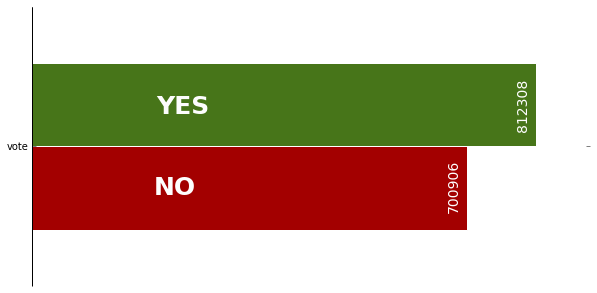
\includegraphics[width=0.6\textwidth]{figures/TABOR_vote}
\end{figure}



\subsection{What is the Purpose of this Inquiry?\label{sub:ResearchObjectives}}

The purpose of this study writ large is to explore the endogenous
role of fiscal institutions in emergent fiscal outcomes. The class
of institutions studied here, tax and expenditure limitations, act
directly on fiscal outcomes by restricting the set of feasible choices
for revenue generation and the allocation of public funds. These institutions,
however, are generally enacted as a response to dissatisfaction with
realized fiscal outcomes. It would be reasonable to push this point
further: the magnitude of the restriction bears some relationship
to the extent of the dissatisfaction.

Such endogeneity is notoriously difficult to untangle, even when the
scope of the phenomenon under study is restricted. In the case of
tax and expenditure limitations, there are many moving parts. TELs
typically have broad application, affecting jurisdictions with wide
variation in socioeconomic circumstance and constituent preference.
Each of these jurisdictions differs in its revenue portfolio, as well
as the complexity and scope of its expenditure responsibilities. Furthermore,
each of these subsystems is vulnerable to the whims of macro-level
fluctuations in economic activity and legal structure. Analytic tractability
requires a reduction in the data space, so that we may tie together
a plausible model of the world. This reduction is necessary in any
rigorous analysis, but endogeneity is not making the task any easier.

For this reason, we identify three broad objectives:
\begin{enumerate}
\item Evaluate the impact of TELs on revenue yield and capacity;
\item Evaluate the extent to which TELs impact expenditure choices; and,
\item Explore whether or not TELs help to align voter preferences with fiscal
outcomes.
\end{enumerate}
In general, it would be reasonable to classify this analysis as firmly
in the political economic arena. As will be discussed, TELs are blunt
instruments. Their popularity, given this lack of surgical precision,
is curious to say the least. This study aims to shed light on why
these policies are enacted. The upfront material and even the first
two empirical sections (revenue and expenditure impacts, respectively)
may be viewed as context for this motivating inquiry. The approach
taken seeks to understand the drivers of votes that exempt counties
from the strictures of TABOR, but these drivers cannot be comprehended
without understanding the impacts of TELs on local public finance
\emph{and how those impacts vary across counties with differing socioeconomic
circumstances.} The fiscal circumstances of a given county contain
information not only about the material resources available to that
county, but also information about the preferences of county voters.
These two informational inputs are difficult to separate from each
other and voter outcomes. What follows does not speak to the separation
of resources and preference, but it does attempt to address the endogeneity
issue by using a predictive framework that incorporates the county-specific
stress faced by the counties in the sample. 


\subsection{What is the Value Added?\label{sub:ValueAdd}}

This kind of analysis is not novel in a broad sense. As we will see,
there exists a formidable literature on TELs. There are two major
elements that differentiate this study from those that have preceded
it. First, rather than focus on a single policy (e.g. TABOR), this
analysis models the joint impact of overlapping policies. The most
novel element of this approach is abstraction away from the explicit
program elements. Previous studies have often modeled the existence
of TELs with binary indicators, or built an index score based upon
factors like method of passage (statutory vs. constitutional), ease
of override, and the magnitude of the growth ceiling among other things.
Unless we believe that the impacts of TELs are additive, binary approaches
lack the informational resolution to model the joint impacts of overlapping
policies. 

Index methods, on the other hand, have a commensurability problem.
Just because one TEL has a statutory authorization and another has
a constitutional authorization, is the former fundamentally less restrictive
than the latter in all cases? Even if we roll all elements of the
index into the equation, does an override procedure have universal
impact irrespective of the joint distribution of remaining TEL components?
Both the binary and index approaches also suffer from lack of variation
in the impact across jurisdictions. The restrictiveness of TELs, as
we will see, is quite dependent upon the circumstances of the constrained
jurisdiction.

For all of these reasons, this study attacks the issue from a novel
perspective. To operationalize these policies,\emph{ the focus is
shifted from program design to program impact}. Instead of asking
how a TEL was passed, for example, we ask what is the feasible levy
given the existence of the policy? This approach rests on a constraint
function that carries arguments for revenue impact and jurisdiction-specific
characteristics. In so doing, it avoids implicit assumptions about
commensurability, facilitates modeling of joint impact for multiple
policies, and provides continuous variation across jurisdictions.
Ultimately, the aforementioned deficiencies are hard to overcome,
and indeed, this study makes an imperfect attempt. We will still have
to make some assumptions that are less than desirable. However, the
philosophy followed here suggests that more is knowable about the
impact of TELs on specific jurisdictions, and we should use that information
to the extent possible.

The second major innovation in the world of TEL research is the explicit
acknowledgement of spatial dependency. No jurisdiction operates in
a vacuum. By virtue of the fact that this study evaluates the impact
of state-enacted policies on local governments, the very design suggests
that vertical relationships across governmental entities matter. Horizontal
relationships are also important components of the system. As it turns
out, externalities are real. The impact of one jurisdiction influences,
and is influenced by, the actions of jurisdictions in the local neighborhood.\footnote{The local neighborhood represents jurisdictions that are ``close''
to the jurisdiction in question. What it means to be ``close'' varies
by analytic objective. For our purposes, we use local neighborhood
to mean the jurisdictions that are spatially proximate. For a different
purpose, one might alternatively define ``close'' to be similarity
in industrial base, or demographic composition, or some other variable
set of interest.} In a manner quite similar to omission of temporal dependency, omitting
spatial dependency can lead to false signals. Does a given jurisdiction
respond to the TEL constraint as the spatially-static model suggests,
or is the measured response a function of the actions of neighbors?
The smaller the jurisdiction, the greater the influence of overlapping
populations, commercial activity, and shared resources.

The flexibility afforded by policy abstraction and the reduction in
error associated with county-specific stress indicators along with
the modeling of spatial dependence clearly separate this analysis
from those that have preceded it. Whether or not these innovations
change the picture painted by previous literature, they seek to account
for potentially confounding elements in the measurement space. In
so doing, agreement would serve only to bolster the robustness of
earlier findings. More importantly, however, these approaches (of
which this study provides only a test drive) open the door for a wider
scope of inquiry than was available with the binary and index approaches.
In particular, the incorporation of jurisdictional variation in impact
helps local policymakers to better understand policy implications
for their own specific circumstance.


\subsection{What is the Spatial Scope of Analysis?\label{sub:SpatialScope}}

The geographic scope of this study is the State of Colorado. It was
chosen because it features what is widely regarded as one of the most
restrictive TEL regimes in the United States. TABOR, specifically,
is often mentioned in the same breath as California's Proposition
13 and Massachusetts' Proposition 2$\frac{1}{2}$ when describing
what a restrictive regime looks like. That being said, TABOR is just
one piece of the puzzle. The TEL landscape also includes the Gallagher
Amendment (GA) and the Statewide Limitation on Property Tax Revenue
(SLPTR), two additional restrictions that act upon local governments.\footnote{Colorado features additional restrictions like Amendment 23 and policies
acting on the state level. This analysis, thus, represents only a
partial representation of the entire landscape.} All three of these policies have significant implications for the
property tax, which is the dominant element of own-source revenue
for local governments in the state. As a consequence of this intersection,
the impact on property tax revenue is the dominant focus for operationalizing
the impact of these policies.\footnote{So enters an implicit assumption that is less than ideal. TABOR actually
has broader revenue scope than SLPTR and GA, but the construction
of the composite constraint used in the empirical modeling requires
a common object upon which the policies can act. The property tax
serves that role, and therefore acts as a proxy in the TABOR case
for the dynamics associated with the broader revenue portfolio.}

Counties serve as the unit of analysis for a number of reasons. First,
general purpose jurisdictions are convenient insofar as they feature
greater variety in service responsibilities. To understand the impact
of TELs on expenditure behavior (the second research objective), this
variation will prove useful because it facilitates identification
of differential impacts from TELs. Suppose an extreme case in which
we have classified expenditure behavior into only high and low expenditure
categories. We may be able to extract a good sense of the likelihood
of a TEL pushing a jurisdiction into one category or the other, but
determining the precise magnitude of the shift is less straightforward.
Increasing the number of categories or switching to interval expenditure
data\footnote{Switching from categorical to interval data is effectively equivalent
to increasing the number of categories, $n\rightarrow\infty$.} helps us answer that question. Splitting the expenditure into more
functions refines our understanding even better.

Second, counties are favored over municipalities for reasons of spatial
parsimony. There are 62 counties in Colorado, and two consolidated
city-county governments (Denver and Broomfield). For the purposes
of this study, Denver and Broomfield are also treated as counties.
This choice reflects the fact that Denver and Broomfield\footnote{According to the Bureau of Economic Analysis, Broomfield County was
created from parts of Adams, Boulder, Jefferson, and Weld counties
effective November 15, 2001. Estimates from BEA for Broomfield began
in 2002.} do not overlap, nor are they overlapped by, the conventional counties
in the state. Moreover, this collection of 64 jurisdictions represents
a spatially-exhaustive set of jurisdictional units. Municipalities
do not feature these properties, nor do they consistently nest within
counties. Thus, the use of municipalities would complicate the analysis
substantially.

The third reason, and perhaps the most important, relates to the allocation
of levy responsibility for the property tax. As we will see, property
taxes are the dominant form of own-source revenue. Counties generally
collect a greater share of property taxes relative to the other major
general purpose jurisdictional form: municipalities.

Finally, counties are also analytically convenient from a data availability
standpoint. Data are collected extensively at the county-level by
both state and federal statistical authorities. At the state level,
the information used in this study is collected by the Colorado State
Division of Local Affairs. They provide excellent, standardized fiscal
information and limited demographic information over the study window.
The federal sources (predominately the US Census Bureau) do not feature
the same reporting frequency in some cases, but the set of socioeconomic
variables is much greater than that which is collected by the state.


\subsection{What is the Significance of the Study Period?\label{sub:StudyPeriod}}

This study examines the fiscal response of counties to TELs over the
1993-2009 time period. The start date reflects the first year in which
all three TELs of interest (TABOR, GA, and SLPTR) acted upon the counties
in Colorado. The end date, by contrast, reflects a less conceptually
relevant rationale. At the start of the this inquiry, the latest available
data in the Colorado County and Municipal Financial Compendium was
for 2009.\footnote{In Colorado, all county fiscal years coincide with the calendar year.}
The subsequent dataset build was then based upon this window.


\subsection{A Word on TELs as an Instrument of Democracy\label{sub:TELs-as-democracy}}

It will become apparent in what follows that TELs are much like sledgehammers.
If binding, they can have large effects on the fiscal behavior of
affected jurisdictions, producing foundational shifts in the trajectories
of revenues and expenditures. Precision, however, is not the a major
strength of the approach. They can just as easily create structural
imbalances as combat waste, fraud and abuse perpetuated by local officials.
And yet, by all accounts, they are quite popular. The student of fiscal
affairs must consider why this is the case.

Canonical public finance is taught from a perspective of the state
as an exogenous actor. The unfettered market, while a remarkably useful
mechanism, is characterized by certain problematic defects that limit
its ability to produce desirable outcomes. Public policy is typically
proposed\emph{ to counteract these market failures.} The very idea
that such a thing is possible requires a belief in our ability to
objectively observe and diagnose a problem, and redirect activity.
It requires a belief in the ability of the state to act on the economy
from the outside. The orthodox question is\emph{ should the state
act} given the existence of both market and government failures? It
is not\emph{ can the state act} on the market?

Buchanan and Tullock, acting as critics of state action, begin to
depart from this premise in the\emph{ Calculus of Consent.}\footnote{Their viewpoint could still be framed in a public versus private context.
In reality, this is a gross oversimplification. It is convenient to
frame the tradeoffs between private and public action as two forces
acting against each other, but Buchanan did in fact view the state
as solely a collection of rules and institutions, as is made clear
in the appendix of the 2004 reprinting of the book (published by Liberty
Fund, Inc). This conception was critical to his distinction between
positive and normative theories of politics.
\begin{quotation}
``A positive science of politics should analyze the operation of
an existing, or a postulated, set of rules for collective decision-making
quite independent of the efficacy of this set in furthering or in
promoting certain 'social goals'. A normative theory of politics should,
by contrast, array the alternative sets of rules in accordance with
their predicted efficiency in producing certain ends or goals which
should be, if possible, made quite explicit.''
\end{quotation}
One need not align with Buchanan's normative assessments to find value
in this methodological split.}
\begin{quotation}
``The orthodox approach does not, however, lend itself well to a
comparative evaluation of different methods of organizing activity.
If we wish to compare collective organization with private organization,
and especially if we want to analyze various collective decision-making
rules, we need, even at the conceptual level, some means of comparing
the\emph{ net} direct gains or the\emph{ net} direct costs of collective
action with the\emph{ costs of organization} itself, that is, with\emph{
the costs of organizing decisions collectively {[}...{]}.}''\citep{Buchanan_Tullock1962}
\end{quotation}
The analysis in this study is generally built on the orthodox view,
but we should at least momentarily consider a reframing of public
action that may make the proliferation of TELs somewhat easier to
understand. Richard Wagner suggests that perhaps it is inappropriate
to think of the market and state as actors.\citep{Wagner2009} Neither
construct actually does anything at all. Rather, they are regulatory
constructs the govern the allowable actions of people who operate
within them. To borrow his terminology, they are not actors, but fora.

When viewed from this angle,\emph{ the state can only ``act'' on
the market if the two fora are populated by different people.} The
ability to separate these groups is a function of the governance structure
that prevails in a society at a given time. Monarchy serves as the
primary example of a governance structure that allows for separability.
Indeed, Wagner suggests that our monarchal roots are the cause for
the orthodox view. In a democratic society, however, separability
does not hold. The same people operate in both the state and market
fora. The only distinction is that each forum has its own set of operational
rules that differentiate how each facilitates the extraction and processing
of resources into services for the public.

Viewed from this angle, the task of the state does not exist. The
task of the public is to design state rules that better align services
rendered with its preferences, from within the existing, yet mutable,
set of rules\emph{.} Institutional rules are complex and, importantly,
are not conducive to smooth adjustment as a function of societal welfare.
That is, there is no straightforward way to change the rules in a
way that maps exactly to the optimal welfare value for a collection
of people. If a jurisdiction increases taxes on cigarettes, the measurement
of the welfare impact must take into account consumers, producers,
and all of the market participants' auxiliary activity related to
the production and consumption of cigarettes. This view is complicated
by knock on effects, as well as the existence and regulation of many
other products and services. Furthermore, it turns out that welfare
is difficult to measure to begin with.

Choice of rules must also contend with the issue of degradation. For
its noble beginnings and the important benefits still conferred today,
the American version of democracy is not without its challenges. To
choose only one aspect, equal representation is more easily idealized
than realized. In the modern political age, it has become clear that
even the definition of equal representation is fairly unclear. At
the base, we can all agree on a single vote for each voter. The ability,
however, to influence the agenda confers great benefits on those who
successfully leverage said influence. Attempts to limit that power,
however, are hamstrung by the need to apply rules in a general way.
Designing rules that do not also abridge basic rights is a significant
challenge.

In this context, ballot initiatives like those that produce tax and
expenditure limitations, blunt as though they may be, emerge as a
method of circumventing the agenda setting power of established interest
groups that have refined their ability to influence the policymaking
process. They are seen as enhancing the role of the public in a democratic
mechanism that must deal with some thorny issues. To be sure, interest
groups have strong influence in promoting the passage or failure of
these initiatives. From the perspective of the voter, however, the
at least apparent civic return may outweigh any lack of precision
associated with the instruments. Furthermore, and this is important,
even if the mix of outcomes is not quite right, the central tendency
may be more in line with the voter's preference than the outcomes
generated by conventional means. Whether or not all of the variables
are appropriately weighed in decisions about these tradeoffs is an
empirical question.


\section{Layout of the Inquiry\label{sec:Layout}}

{*}{*}{*}CHAPTER REFS AREN'T WORKING???

Before any empirical testing, it is important to provide information
about the operating context. Chapter \ref{chap:SubFinUS} provides
an overview of subnational finance in the US. In particular, the presented
perspective seeks to provide broad justification for studying subnational
fiscal institutions. Furthermore, the Appendix extends this discussion
with an overview fiscal institutions in general. This study, of course,
focuses on tax and expenditure limitations specifically. Chapter \ref{chap:CO-FiscBehavior}
explores the fiscal structure of Colorado, and the socioeconomic context
for the study period. The chapter concludes with a detailed discussion
of TELs in Colorado, and how this study attempts to operationalize
them.

Given the context, the next three chapters address aspects of the
research objectives detailed in Subsection \ref{sub:ResearchObjectives}.
Chapter \ref{chap:RevYieldCapacity} explores the extent to which
TELs in Colorado (COTELs) impact revenue yield and capacity at the
county level. To the extent that COTELs modify the ability to collect
revenue, these policies impact a county's capacity to deliver public
services. Chapter \ref{chap:ExpPatterns} tests whether or not the
intensity of COTEL constraints is associated with a deflection in
the expenditure behavior of a given county. Such a deflection would
affect the ability of a county to provide services that are consistent
with constituent preferences. Both Chapter \ref{chap:RevYieldCapacity}
and Chapter \ref{chap:Expenditure-Patterns} are essentially explorations
of the transactional nature of local public service consumption, the
``duality'' of public finance at the local level. With this context,
Chapter \ref{chap:DeBrucing} changes directions to partially explore
TELs as an instrument of democracy. The big question, as identified
in Subsection \ref{sub:ResearchObjectives}, is whether or not TELs
can align fiscal outcomes with voter preferences. Before such a question
can be answered, we must know what voter preferences are. This last
empirical chapter tests local overrides (i.e. ``DeBrucing'')\footnote{Douglas Bruce is a former lawmaker in Colorado, and the principal
author of the Taxpayers' Bill of Rights (TABOR). Having been remarkably
persistent in pushing the policy through, he has largely been seen
as the public face of TABOR. Consequently, votes conducted by localities
to exempt themselves from the strictures of TABOR for at least a limited
amount of time have come to be known as ``DeBrucing'' efforts.} as an instrument of revealed voter preference.

Chapter \ref{chap:Conclusion} contains the conclusion. It presents
final thoughts on what has been learned in the empricial testing and
seeks to weave the findings together to see what may be said of TELs
in Colorado. It will also include discussion of the extent of the
study's external validity, as well as thoughts on what may be explored
with future research.

\clearpage


\chapter{Subnational Finance in the United States\label{chap:SubFinUS}}

The federal system of government in the United States is arguably
among the most complex social coordinating mechanisms in the world.
It is comprised of over 90,000 individual governmental entitites\footnote{According to the US Census Bureau, as of 2012, there were 90,106 state
and local governments.\citealt{COG_Summary2012}} characterized by hierarchical, overlapping, and irregular spatial
arrangements. The national and state governments account for only
51 of these entities. Aside from a handful of territories, the remaining
entities constitute the remarkably diverse local government sector.
In broad terms, to borrow the Census classification, these governmental
units are split into five classes: counties, municipalities, townships,
school districts and special districts. These local governments vary
in population size and composition, resource endowment, geographic
scope, corporate purpose, and the nature by which they interact with
vertical and horizontal counterparts.


\section{Why are the Fiscal Affairs of States and Localities Important?}

In his treatise,\emph{ The Theory of Public Finaince} (\citep{Musgrave59}),
Professor Musgrave constructed a framework for conceptualizing public
finance in a federal system that has proven robust to a remarkably
varied set of research inquiries. This framework once again proves
useful in explaining the significance of subnational finance in the
US. Musgrave's approach defines three primary tasks for the public
sector in an economy, and allocates those functions to the appropriate
level of government. For the purposes of this analysis, the front
end of the framework (function definition) proves directly applicable
while some modification of the back end (allocation of functions)
may be needed.

According to Musgrave, there are three primary roles for the public
sector:
\begin{itemize}
\item Direct service delivery (i.e. allocation);
\item Redistribution of resources; and,
\item Macroeconomic stabilization.
\end{itemize}
The first (allocation) is the direct product of government operation,
the most direct link to taxes paid. The second (redistribution) seeks
to adjust resource allocations to accord with societal preferences
for distributional equity. An additional motivation for this function
can be the mitigation of damages that have occured due to trade. Insofar
as the cost-benefit calculation from a trade is typically considered
beneficial whether or not the gains help to offset the losses experienced
by ill-placed parties\citep{Hicks39,Kaldor39}, losses are free to
occur by construction. The third function (stabilization) seeks to
maintain an environment conducive to achieving the full potential
of economic output.

As it turns out, these three functions cannot be cleanly assigned
to the three levels of government (federal, state, and local). Indeed,
comparatively recent literature\citep{Bahl1984,Gramlich1993} suggests
that the discord is even greater than Musgrave had originally believed.
In any event, there is broad agreement that the preponderance of direct
service provision occurs at the level closest to the recipients of
services: local. Indeed, this de facto postulate is the supporting
force behind Oates' Decentralization Theorem\citep{Oates1972}\footnote{It should be noted that Professor Oates would argue, and has argued
(\citep{Oates2008}), that Tiebout sorting is not a prerequisite for
the Decentralization Theorem. Mobility is not required for the latter
to have an effect. I would argue, however, that even if unnecessary,
Tiebout sorting improves the efficacy of the Decentralization Theorem
in the sense that mobility increases the systemic capacity to match
supply and demand in the local taxation-expenditure bundle market.}:
\begin{quotation}
``For a public good - the consumption of which is defined over geographical
subsets of the total population, and for which the costs of providing
each level of the good are the same for the central or for the respective
local government - it will always be more efficient (or at least as
efficient) for local governments to provide Pareto-efficient levels
of output for their respective jurisdictions than for the central
government to provide any specified and uniform level of output across
all jurisdictions.''
\end{quotation}
Perusal of budgets across the three levels of government will affirm
that direct service provision constitutes larger portions of the budget
the closer one gets to the citizens. This is a good thing because
the capacity to choose among local menus is welfare enhancing.

Direct service provision serves as the nexus at which the taxpayer
realizes the connection between tax price and the return from that
investment. Indeeed, this intuitive dictum accords with an argument
that substantially predates Musgraves' revelation. The nascent stages
of our republic were characterized by fierce deliberation over the
capacity to govern such a geographically expansive jurisdiction. The
concern raised by so-called ``Anti-Federalists'' was the idea that
it was simply not possible to govern a space of this size because
representatives could not feasibly identify with the populations they
were elected to represent.\citep{Storing1981} Again, the issue was
contact. Supporting direct service delivery (a role that is critical
not only to public finance, but also democracy) requires a vehicle
by which said activities can propagate. That is, the resources to
deliver these services must be reliably generated from a viable and
stable revenue source.


\subsection{What Normative Objectives Should be Pursued in a System of Subnational
Finance?\label{sub:SubFinance-Normative-Objectives}}


\subsubsection{The Importance of Local Autonomy}

While it is true that the proliferation of idiosyncratic elements
across local governments creates challenges in coordination, the variety
is actually an asset.\citep{Tiebout1956} It is this variety that
provides a vehicle for demand articulation within the public sphere.
Insofar as taxpayers are free to choose among a set of taxation-expenditure
bundles, the system intrinsically seeks to minimize the deadweight
loss associated with coerced conformity. Tiebout sorting requires
some unrealistic assumptions in perfect information and costless mobility,
but there does appear to be empirical support for the occurrence of
sorting. The following draws upon the review of voting and sorting
literature performed by Stephen Ross and John Yinger\citep{Ross_Yinger1999}:
\begin{itemize}
\item Individual jurisdictions are far more homogenous than the urban area
in which they are contained\citep{Pack_Pack1977};
\item Within-jurisdiction homogeneity increases with the number of jurisdictions\citep{Hamilton_Mills_Puryear1975,Eberts_Gronberg1981};
\item Census tracts of similar types are likely to be found within the same
jurisdictions\citep{Heikkila1996}; and,
\item Surveyed households within jurisdictions show statistically relevant
alignment in preferences about the appropriate level of public services.\citep{Gramlich_Rubinfeld1982}
\end{itemize}
While this does look promising, Ross and Yinger note that homogeneity
as an observable phenomenon is insufficient to prove sorting because
the observed results are also consistent with the consensus bidding
framework. Schmidt, however, does find evidence that increased income
heterogeneity increases the desired number of school provider types.\citep{Schmidt1992}
This result is consistent with the predictions of the Henderson model\citep{Henderson1991},
which is a derivative of Tiebout's. The implication here (albeit weak)
is that public service preferences, rather than home values, drive
sorting.

An extensive review of the sorting literature is beyond the scope
of this inquiry. However, if we believe the sorting narrative that
has provided the basis for much of the literature over the last half
century, then the capacity to finance a tax-expenditure bundle consistent
with the preferences of the residents in a particular jurisdiction
is essential.

If the means of finance is not available, with what resources can
policymakers respond to the demands of their constituents? Fiscal
autonomy requires the freedom to set expenditures\emph{ and} raise
revenues to finance said expenditures.\citep{Bird1993} Furthermore,
autonomy is driven less by the overall adequacy of revenue as the
control over\emph{ marginal} sources of revenue.\citep{McLure2001}
If total yield was all that mattered, local differentiation would
be far less relevant. The capacity to deviate is what enables accommodation
of local preference.


\subsubsection{Local Tax Design}

Establishing a local tax requires an awareness of both general tax
design and the environment in which the tax is to be levied. Bird
identifies the properties of a good local tax and suggests consumers
of his research seek to equalize benefits and costs at the margin\emph{
when possible}.\footnote{Bird captures the latter suggestion directly: ``Whenever possible,
charge.''}\citep{Bird1993} A truly local tax features four major characteristics:
\begin{enumerate}
\item Local assessment;
\item Local rate setting;
\item Local collection; and,
\item Accrual of proceeds to the local entity.\footnote{Note that the third and fourth characteristics are distinct insofar
as collection is simply an activity, while the absorption of proceeds
dictates where the resources will ultimately reside.}
\end{enumerate}
Having established the operational handles of an abstract local tax,
the choice of specific taxes should strive to capture the ideal elements
of such a tax: immobility, adequacy/buoyancy, stabilty/predictability,
fairness, administrative ease, non-exportality, and visibility (i.e.
transparency). For the most part, these characteristics are goals
for any tax at any level.\footnote{Note that these are theoretical objectives for tax design, identified
for the purpose of maintaining a tight coupling between revenue generation
and expenditure allocation. Such a coupling seeks to create a tight
response for taxpayers, so that they may link the costs they feel
from taxes with the benefits of service delivery in a manner that
minimizes noise from other factors. The stronger this linkage, the
greater the capacity for taxpayers to equalize costs and benefits
at the margin. In practice, however, political expediency has an outsized
role in the selection of available revenue handles, and can distort
the role of other characteristics. For example, from a political perspective,
exportability becomes an asset for those promoting a given tax.}

The property that stands out in the local context is immobility. In
the revenue schema of fiscal federalism established by Oates in 1972\citep{Oates1972}
(and subsequently supported by Bird, Gramlich, and others), the idea
of open and closed jurisdictions plays a prominent role. Closed jurisdictions
are characterized by sufficiently high exit costs as to discourage
departure from the jurisdiction over a wide range of tax prices. While
the national government may feature this property, local governments
do not. Local governments must contend with open borders, also known
as low costs of exit. It is for this reason that a graduated income
tax with comparable progressivity to the national model does not exist
at the subnational level. Local officials are worried that taxpayers
may simply choose to reside somewhere else. In this light, the fixed
nature of real property makes it an attractive base upon which to
levy a local tax.


\subsubsection{Duality in Public Finance\label{sub:Duality-in-Public-Finance}}
\begin{quotation}
``The classical approach to the theory of Public Finance - with its
neglect of the expenditure aspects of public economy and its overemphasis
of the consideration of justice in its treatment of the revenue aspect
of the problem - had left the revenue-expenditure process outside
the body of economic theory.'' - Richard Abel Musgrave, 1939
\end{quotation}
Professor Musgrave described here a concept that dates at least as
far back as Adam Smith's\emph{ Wealth of Nations.\citep{Smith1776}}
Smith's work is probably among the most prominent writings in economics
that advocates for the ability-to-pay principle.\footnote{Adam Smith, himself, did not actually support the neglect of the expenditure
side of public finance in his writings. Rather, this phenomenon was
a product of his successors - McCullock, Nassau Senior, James Mill,
etc. - who distilled Smith's message down to a narrower vision.} While ability-to-pay does well to explicitly address equity concerns,
using the concept as an analytic base facilitates neglect of a fundamental
characteristic of public finance. Musgrave's ``revenue-expenditure
process'', Wagner's ``quid pro quo'' or ``consensual democracy''\citep{Wagner1983},
and Burkhead \& Miner's ``general equilibrium analysis'' or ``balance
sheet'' approach\citep{Burkhead_Miner1971} are all slices at the
same underlying concept: duality.

Revenue systems cannot, and should not, be divorced from the public
services they finance. Though this fact was recognized with the advent
of marginal utility economics (particularly as advanced by Wicksell),
it has not yet made much headway in popular discourse over economic
policy in the United States. Too often we see tax discussions without
thought to programmatic impacts and vice versa. As we will see, this
disconnect has created conditions that drive an even larger wedge
between considerations of public revenue and expenditure.


\section{What does Subnational Finance Look Like in Practice?}

Theoretical knowledge of ``proper'' tax design and a strong appreciation
for the normative role of subnational finance are important from a
foundational perspective. However, theoretical constructs are insufficient
to operate in the real world. The competent fiscal manager requires
knowledge about the characteristics of the revenue bases in question,
trends in base activity and expenditure risk, and the institutions
that govern the linkages between the economic capacity of a given
population and its desired basket of public services. In short, one
must understand the operating context.


\subsection{The Economic Significance of the State and Local Government Sector}

The role of government, as measured by its size relative to the total
economy, has grown signficantly since the beginning of the early 20th
century. Given the comparatively low-level of resources allocated
to the judicial and legislative branches, this growth has been driven
by increases in the executive and regulatory capacity of government
at all levels. Figure \ref{fig:Tot-Gov-Size} depicts the trajectory
of total government receipts and expenditures as a percentage of gross
domestic product. As one might expect, both receipts and expenditures
tell similar stories. Between 1929 and 2013, receipts grew from 10.04\%
of GDP to 28.56\%, while expenditures grew from 8.03\% to 33.77\%.

\begin{figure}
\caption[Government Size]{Growth in the Size of Government\label{fig:Tot-Gov-Size}}


\centering{}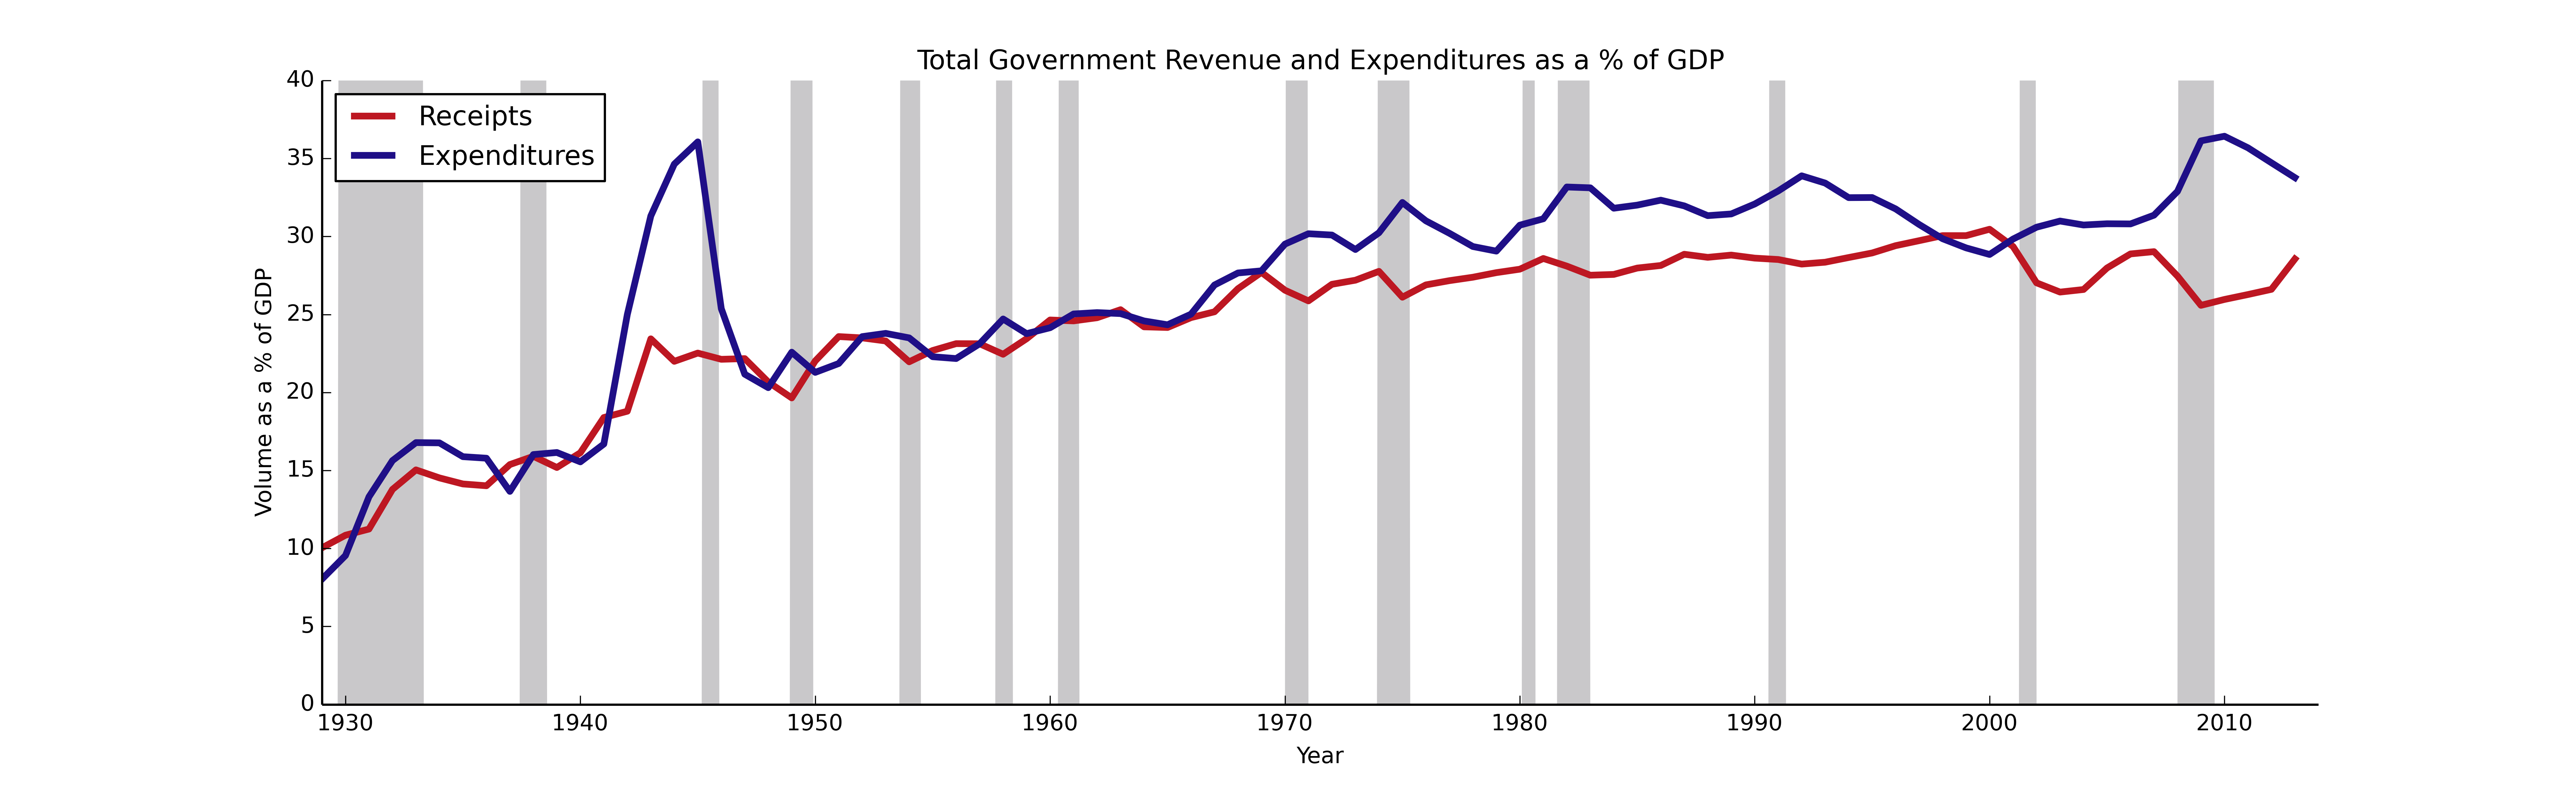
\includegraphics[width=1\textwidth]{figures/tot_gov_GDP_perc}
\end{figure}


This growth reflects the rise of what Dwight Waldo referred to as
the ``administrative state''.\citep{Waldo1948} Although the growth
in government we were to experience in the US was unprecedented, it
was by no means an accident. Rather, it was a consequence of the intersection
between a growing population and the prevailing culture.
\begin{quotation}
``{[}D{]}espite occasional claims that public administration is a
science with principles of universal validity, American public administration
has evolved political theories unmistakeably related to unique economic,
social, governmental, and ideological facts.''\citep{Waldo1948}
\end{quotation}
In effect, the growing population placed a strain on existing methods
of allocating resources and conducting the business of running a country.
Interdependence amongst people was growing, which highlighted the
need for methods of promoting common expectation. If two parties are
to engage in a fruitful manner, some common set of rules is required.
The sheer number of such engagements grows faster than the population\footnote{Consider a population of two people. The addition of a third person
adds not one, but two additional avenues for engagement.}, and the potential for variation in the engagements grows with it.
Furthermore, as the economy matured, industrial activity became more
differentiated, specialized, and technical. Establishing common expectation
in this circumstance requires a regulatory apparatus with specialized
training. Ignorance of this fact was a perilous strategy.\citep{Cleveland1906}
The resource base required for a governmental apparatus to achieve
these efficiencies was larger than had been previously required.

Although the federal government has expanded more rapidly than the
state and local sector, subnational finance still increased its share
of the economy over the course of the past century. Over the 1929-2013
period, Figure \ref{fig:SL-Gov-Size} shows that subnational receipts
grew from 6.79\% of GDP to 12.68\%, while subnational expenditures
grew from 5.45\% to 14.02\%. As can be seen, the sector grew quite
rapidly early on, before a temporary decline in the mid-1930s. Much
of the early experimentation with new methods of administration accordingly
started in state and local governments.

\begin{figure}
\caption[Subnational Government Size]{Growth in the Size of Subnational Government\label{fig:SL-Gov-Size}}


\centering{}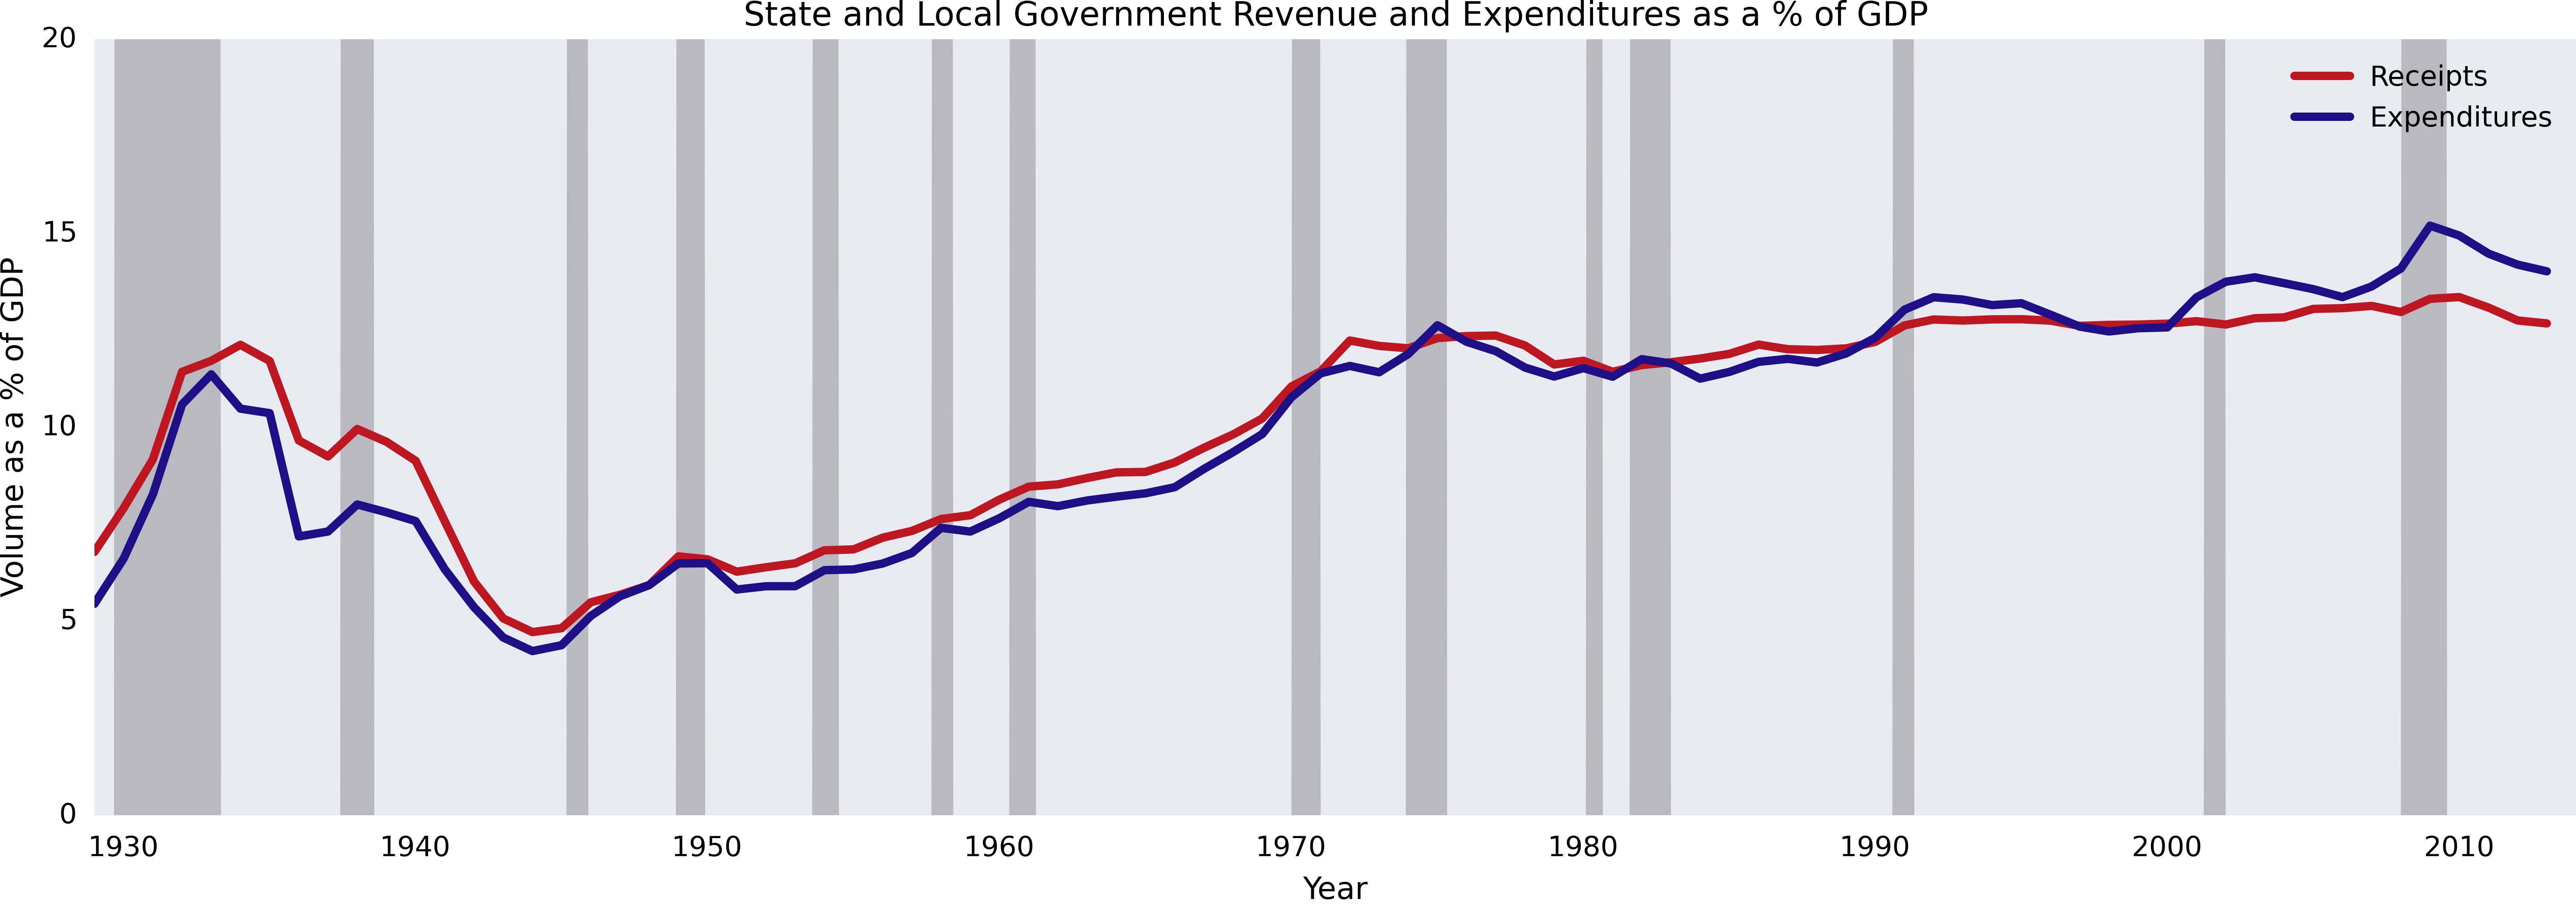
\includegraphics[width=1\textwidth]{figures/sl_gov_GDP_perc}
\end{figure}



\subsection{The Role of the Property Tax in Financing Local Government}

Over the course of US history, financing the array of service responsibilities
contained within any given local government entity has required careful
and ongoing cultivaton of a revenue portfolio that seeks to draw upon
the economic activity contained within (or near) the jurisdiction
in question.\footnote{This characterization encompasses only own-source revenues and not
intergovernmental transfers.} Amongst all revenue options, taxes dominate the space. That being
said, as Figure \ref{fig:Sub-Taxes} shows, their importance has declined
over the past century. Between 1929 and 2013, taxes dropped as a percentage
of total subnational receipts from 90.14\% to 69.24\%.

\begin{figure}
\caption[Subnational Taxes]{Decline in Tax Proportion of Subnational Receipts\label{fig:Sub-Taxes}}


\centering{}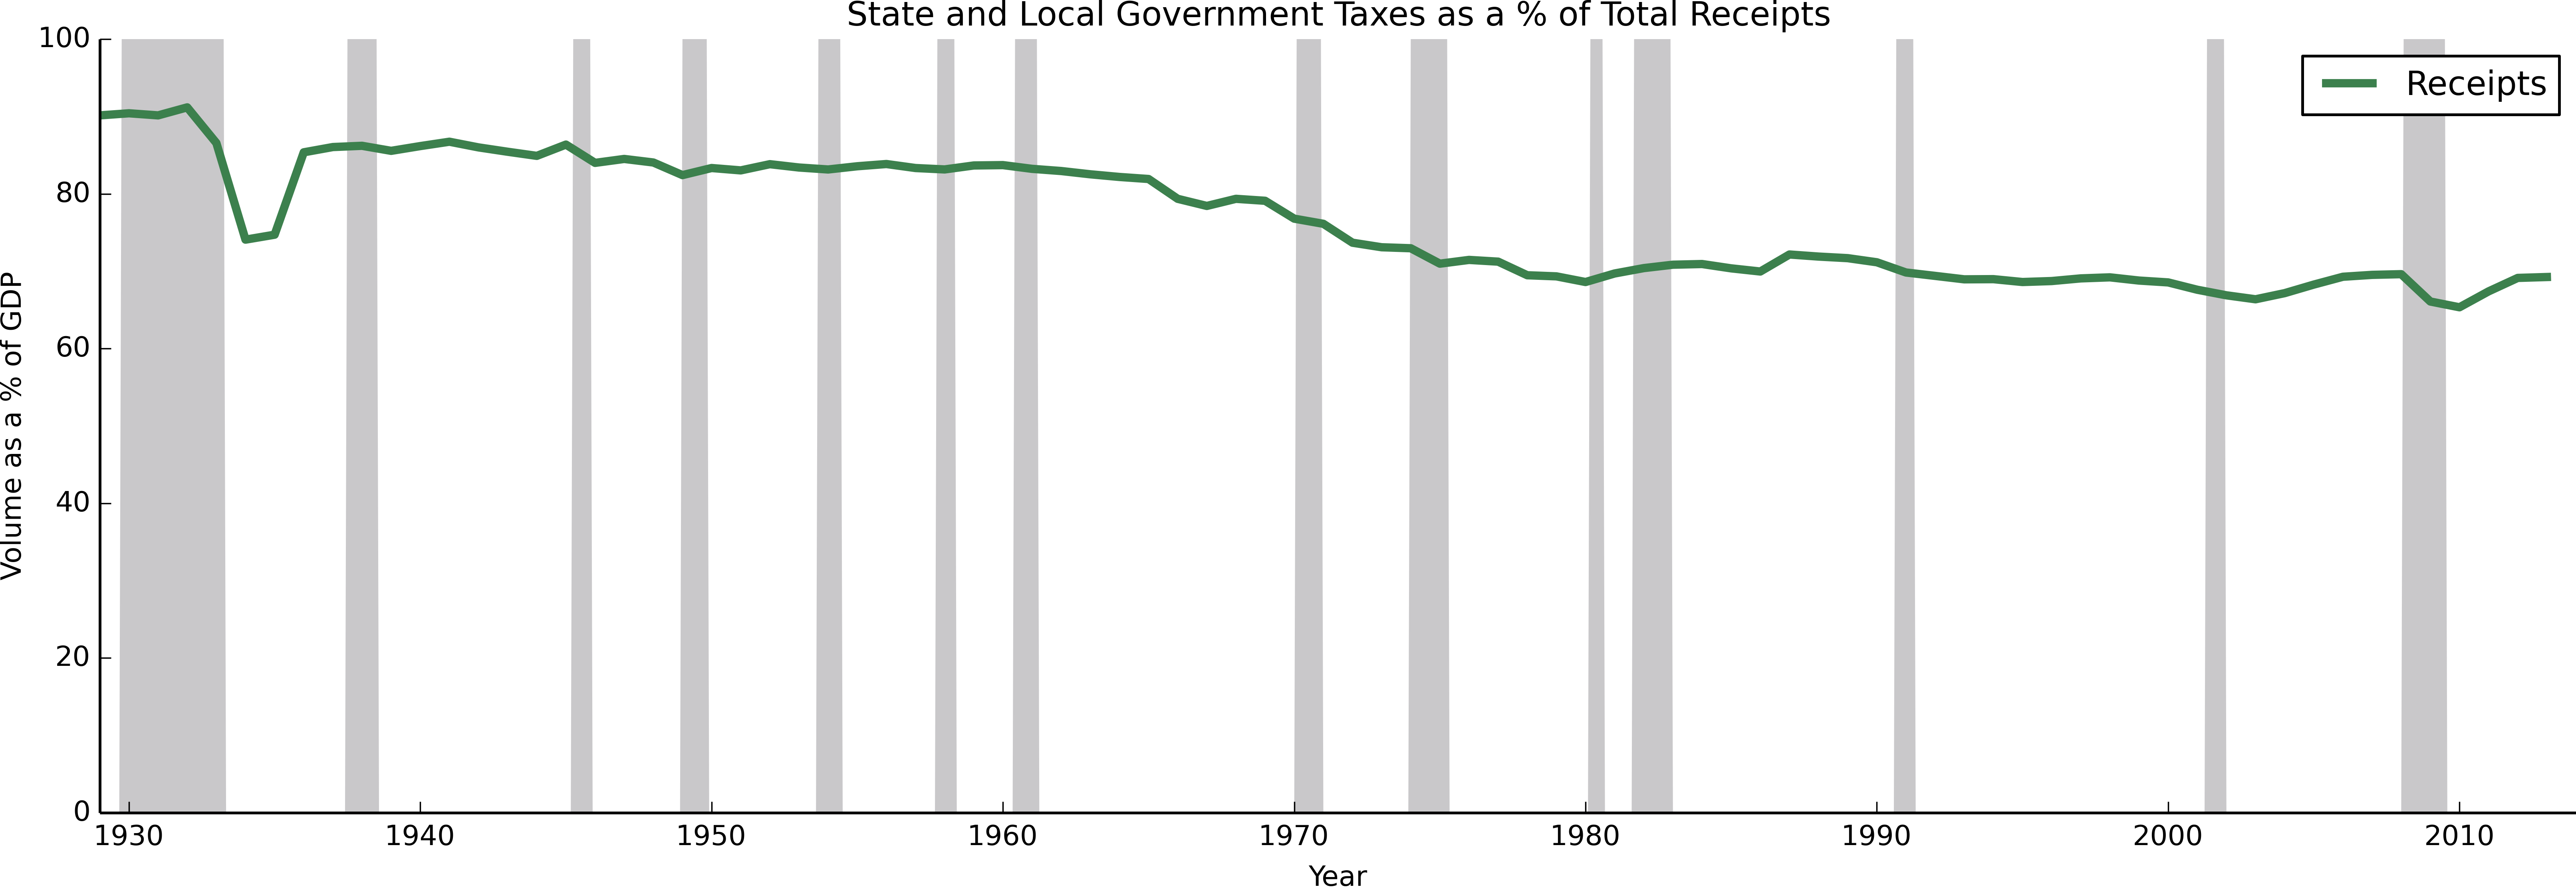
\includegraphics[width=1\textwidth]{figures/sl_tax_perc}
\end{figure}


Focusing on local governments, despite a variety of revenue instruments
from which to choose, one has stood out over time as the dominant
source of local receipts: the taxation of property. This instrument
serves as both the motivation behind, and the primary driver of, the
empirical analysis that follows.

The property tax as an object of study is an immense topic worthy
of the extensive literature devoted to it. This study is specifically
motivated by what has been popularly described as the erosion of the
property tax base. Insofar as they reduce property tax revenue by
construction, the impact of deviations from the property base carry
clear first order effects. The ultimate systemic impact on revenue
performance and utilization is less than clear. It is not known, for
example, whether or not these deviations make the property tax a more
palatable revenue instrument for taxpayers. As noted by Glenn Fisher
\citep{Fisher1996}, there are competing forces at work in a complex
political economic system. The resultant of these forces appears to
require empirical identification. This study does not address this
question per se, but it does explore the related topic of the implications
associated with policies seeking to limit the property tax's scope
of application.

Property taxes have managed to maintain strong yields over time, and
still remain the single largest revenue source for local governments.
This compositional prominence, however, has experienced a notable
decline. Between 1959 and 2012, property tax revenue declined as a
percentage of local current receipts from 53\% to 36\% (Figure \ref{fig:prop-tax}).

\begin{figure}
\caption[Property Tax Decline]{Declining``Importance'' of Property Taxation\label{fig:prop-tax}}


\begin{centering}
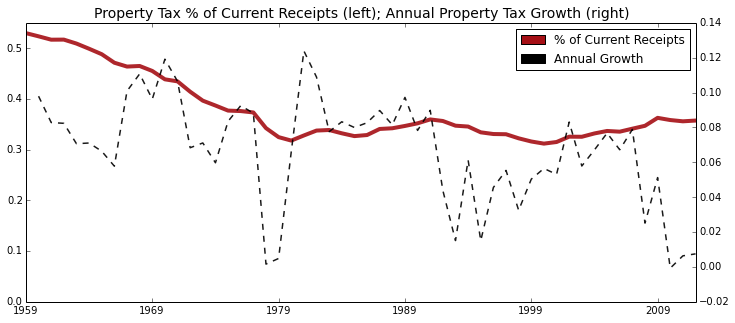
\includegraphics[width=1\textwidth]{figures/NIPA_prop_tax}
\par\end{centering}

Confirm base does actually include intergovernmental transfers....
Include ``local'' tag in exhibit/
\end{figure}


As with the entire state and local sector, we see that the declining
importance of property taxes for local governments coincides with
the declining importance of local taxes generally (Figure \ref{fig:Local-Receipts}).
Tax receipts as a percentage of total current receipts has declined
from 63\% to 50\% over the 1959-2012 time period, offset entirely
by a larger rise in current transfers from other governments (31\%
to 48\%). Within tax receipts, the decline in proportion of property
revenue is still significant, if less dramatic (84\% to72\%). Sales
taxes (7\% to 16\%) and income taxes (1\% to 4\%) have filled the
void. Nevertheless, the continued importance of the property tax cannot
be overstated.

\begin{figure}
\caption[Local Receipts]{Sources of Local Receipts\label{fig:Local-Receipts}}


\begin{centering}
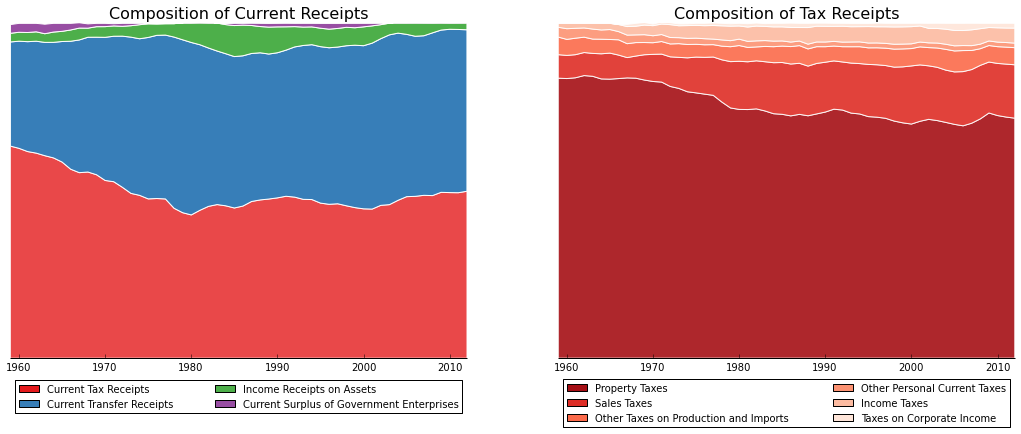
\includegraphics[width=1\textwidth]{figures/NIPA_rev_comp}
\par\end{centering}

Confirm what ``Income Receipts on Assets'' is....
\end{figure}


The decline of the property tax is quite marked beginning in the 1970s.
The likely culprit is the tax revolt that occurred during this period,
which brought a wave of base eroding measures. The impact of this
class of measures on fiscal behavior is the subject of this study.

This so-called tax revolt was the product of a confluence of economic
and social factors. The 1970s saw two recessions, a marked decline
in real GDP growth, and a sharp increase in inflation (Figure \ref{fig:Macroeconomic-Turmoil-in-1970s}).
Citizens still recalled the remarkable expansionary period that had
preceded the decade, a time of growing incomes and a voracious appetite
for social progress. Irene Rubin captures well the environment that
spawned the strong anti-tax sentiment:
\begin{quotation}
``Citizens have often endorsed or even demanded rapid expansion,
but when projects fail, when citizens' incomes lag and they no longer
feel they can afford these projects and programs, or both, they withdraw
their support for additional taxation or try to reduce their tax burden.''
\end{quotation}
The consequence was a wave of reforms, designed to aggressively lower
taxpayers' most visible local liability, the property tax.

\begin{figure}
\caption[Turmoil in the 1970s]{Macroeconomic Turmoil in the 1970s\label{fig:Macroeconomic-Turmoil-in-1970s}}


\centering{}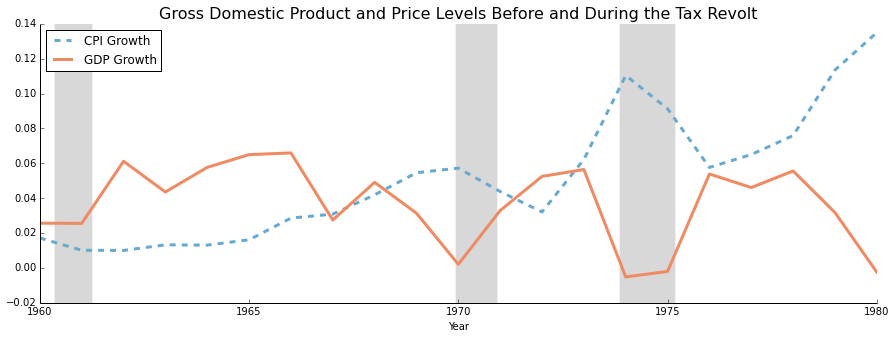
\includegraphics[width=1\textwidth]{figures/cpi_gdp_60_1}
\end{figure}


The implications of these reforms was far-reaching. The central role
played by the property tax makes it a critical tool of fiscal autonomy.
Unlike transders, which rely on the willful participation of other
jurisdictions, taxes are designed by the collecting jurisdiction.
They are thus customizable, tailored to suit said jurisdiction's needs.
As has been demonstrated, the property tax plays a dominant role within
this space.


\subsection{Growth and Volatility Factors in Local Public Finance}
\begin{quotation}
``'Policy handles' are merely levers that local officials can use
to adjust at the margin the fiscal health of their local governments
as opposed to precision tools that can bend and shape the environment
to their will.''\citep{Honadle_Costa_Cigler2004}

\begin{figure}
\caption[Local Strategies]{Strategies of the Local Fiscal Manager\label{fig:Loc-Fisc-Strategy}}


\centering{}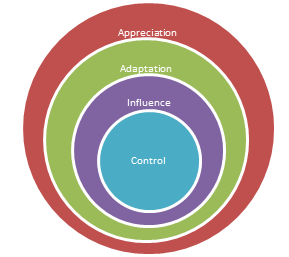
\includegraphics[width=0.7\textwidth]{figures/official_handles}
\end{figure}


Figure \ref{fig:Loc-Fisc-Strategy}\footnote{The figure is a recreation of Honadle et al.'s adaptation of the framework
developed by Smith and Thoolen.\citep{Smith_Thoolen1980}} represents the strategies that a local fiscal manager can take to
effect changes in the operations of his/her jurisdiction. The size
of each circle reflects the amount of opportunity the manager has
to pursue such a strategy. Note that the smallest circle contains
the ``Control'' strategy. The interpretation is that there are few
scenarios in which the local fiscal manager has complete deterministic
control over the outcome of a particular policy. One example of such
an opportunity would be the selection and implementation of the accounting
system used to track receipts collected by the jurisdiction's tax
authority. With each successively larger circle, the subset of variables
controlled by the manager for a given policy outcome decreases. The
largest circle, the ``Appreciation'' strategy, captures those outcomes
for which the manager has almost no control at all. A decision by
the state to cut state aid to local governments would likely fall
into this category. The implication of the small area allocated to
``Control'' is that very little of the forces that act upon a local
government are under the control of the manager, creating a tumultuous
environment for fiscal responsibility. It is this uncertainty, the
details of which will be elaborated upon shortly, that drives the
need for a stable and reliable revenue portfolio.

Tax and expenditure limitations would fall within the ``Adaptation''
sphere. In our case (Colorado), they are imposed by the state on local
authorities. The impacts of these policies are mitigated only by utilizing
supplemental revenue sources, or successful execution of a local override
(``deBrucing''). In general, local authorities have little opportunity
to avoid these policies completely.
\end{quotation}

\subsection{The Importance of Demography}

One of the primary challenges facing fiscal managers at any level
of government in the US is the deomgraphic shift that is occurring
in the country. For local managers, there are three key areas that
must always figure prominently in planning for the future: the senior
population, school age children, and migratory patterns.\citep{Honadle_Costa_Cigler2004}
The first two deal directly with the provision of expensive services
while the last drives both expenditure and revenue side concerns.
At the current time, the imminent growth in the senior proportion
of the population represents the elephant in the room:
\begin{quotation}
``{[}T{]}he growing debt {[}...{]} reflects an imbalance between
spending and revenues that predated the recession. Whether that debt
will continue to grow in the coming decades will be affected by not
only long-term demographic and economic trends but also by the policymakers'
decsions about taxes and spending. The aging of the baby boom generation
portends a significant and sustained increase in the share of the
population receiving benefits from Social Security and Medicaid, as
well as long-term care services financed by Medicaid. Moreover, per
capita spending for health care is likely to continue rising faster
than spending per person on other goods and services for many years
{[}...{]}.''\citep{CBO_LTBO2012}
\end{quotation}
While healthcare spending growth has actually slowed significantly
in recent years\citep{Cutler_Sahni2013}, the point is still a salient
one with respect to drivers of fiscal exposure. Furthermore, provision
of economic security in the ``out years'' of life is not a new concept.\footnote{One can find a history of the concept on the Social Security Administration's
website.} The idea is fundamentally based upon the insurance concept and it
dates back to the Ancient Greeks who stockpiled olive oil to fortify
themselves against fluctuations in the economy. The modern US Social
Security program was initiated in 1935. The life expectancy in that
year was 61.7 years\citep{Arias2012}; the earliest benefits from
the program are payable at 62 years of age.

\begin{figure}
\caption[Age Distribution]{Trends in the US Age Distribution\label{fig:Age-Distribution}}


\begin{centering}
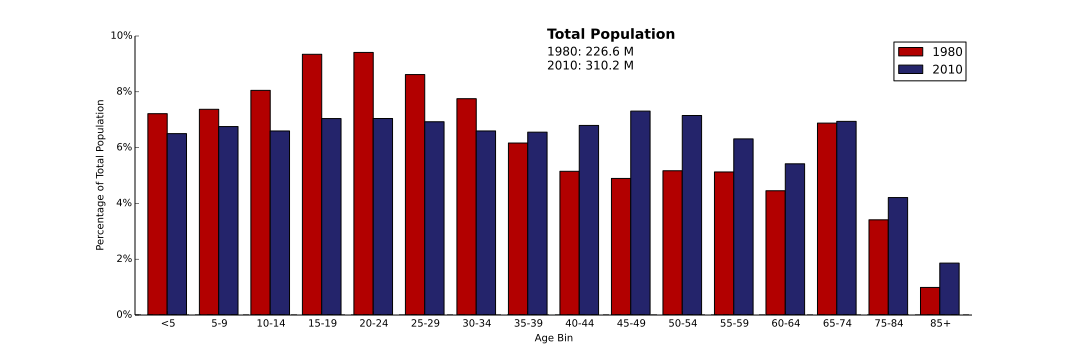
\includegraphics[width=1\textwidth]{figures/Ch2_pop_trend}
\par\end{centering}

Replace with dependency ratio (include children)....
\end{figure}


Medicare is essentially a healthcare-specific variant of the same
concept. Congress initiated this program in 1965, a year in which
life expectancy in the US was 70.2 years. This program pays out full
benefits at age 65. Both Social Security and Medicare have grown substantially
as a function of improving health outcomes, and this effect is exacerbated
by bulges in the age distribution. In particular, the ``Baby Boomer''
generation has already begun to place considerable strain on the solvency
of these initiatives.

This macro-level environment has direct and indirect consequences
for local fiscal managers. The first direct impact involves increased
expenditure exposure in functions related to emergency services and
any funding for senior care. The second direct impact reduces receipts
by way of senior-related tax non-neutralities (e.g. property tax credits
for seniors). Indirect impacts are driven by increased expenditure
risk for governments at the state and federal level. To the extent
that the administration of these programs reduces the available funding
for aid to local governments, the local fiscal manager must find creative
solutions to funding shortfalls.


\subsection{The Evolution of the Economy}

One of the greatest challenges facing local jurisdictions is the evolution
of the economy. The well-recognized trend away from hard goods production
to services\citep{Stiglitz2012} undermines the traditional revenue
handles held by local governments. As mentioned previously, one of
the most critical aspects of a local revenue portfolio is a reliable,
and preferably,\emph{ immobile} revenue source. The immobility of
the property tax base, for instance, derives much of its value from
the decision of economic actors to site themselves within the jurisdiction
in question. To the extent that economic coordination requires spatially
proximate association to a decreasing degree, local governments are
losing the capacity to leverage this siting choice. Even if the country
as a whole experienced no net loss in population, those local jurisdictions
with comparatively high revenue requirements stand to lose a great
deal. Beyond that, siting within the US in general is not quite as
necessary as it was at one time.

This phenomenon is not entirely driven, however, by revenues. Before
any consideration of remote coordination occurs, jurisdictions must
have the capacity to support it:
\begin{quotation}
``An information-based economy that is fueled by advanced telecommunications
may mean that small cities and rural areas - many already with declining
population and job bases - lose locational advantages derived from
proximity to railroads or water.''\citep{Honadle_Costa_Cigler2004}
\end{quotation}
In general, the onset of the information age is catalyzing a fundamental
shift in the nature of economic interaction in this country. This
shift is necessarily coupled with a shift in the relative value of
factor inputs. Strategic governance decisions of the past are, for
many local jurisdictions, becoming liabilities. The challenge for
local officials is to adapt in a manner that retains or recreates
relevance for the their jurisdiction. The transition is costly, placing
further emphasis on the need to safeguard reliable sources of revenue
(even when said sources are plagued by base erosion).


\subsection{Macroeconomic Events}

One of the lessons learned from analysis of local fiscal capacity
is the following:\emph{ successful fiscal operations require anticipation
of, and responsiveness to, macroeconomic shifts.} This issue is particularly
acute at the local level since the available responses are more related
to adaptation than influence. Obviously the capacity for anyone to
anticipate a specific occurrence of an economic downturn is quite
limited. The appropriate course of action is a probabilistic assessment,
coupled with the appropriation of a sufficient multi-year revenue
buffer to help weather the storm.

For the local fiscal manager, the assault on revenues during a recession
comes from multiple fronts. The first, and most direct, impact comes
from the reduced tax collections stemming from a reduction in economic
activity.\footnote{Economic activity, as used here, captures both the value generated
from transactional interactions among economic actors and the change
in capital value associated with said transactions. For example, many
buyers and sellers in a local real estate market generate value with
marginal returns to each transaction on average. Such a market is
also likely to see increases in the value of the housing stock as
a whole. Both are functions of underlying demand, which would be depressed
in a recession.} The second front involves the ``automatic'' fiscal response stemming
from a sharp increase in the dependency ratio.\footnote{In this context, ``dependency ratio'' cost captures increased expenditures
that occur with growth in the impoverished portion of the resident
population. This is in contrast to the traditional age-related definition,
which is defined by the proportion of children and seniors.} The third front is a function of the intergovernmental fiscal transfer
system.

\begin{figure}
\caption[Transfers to Local Governments]{Volume of Intergovernmental Fiscal Transfers to Local Governments\label{fig:Volume-of-IntGov-transfers-to-local}}


\centering{}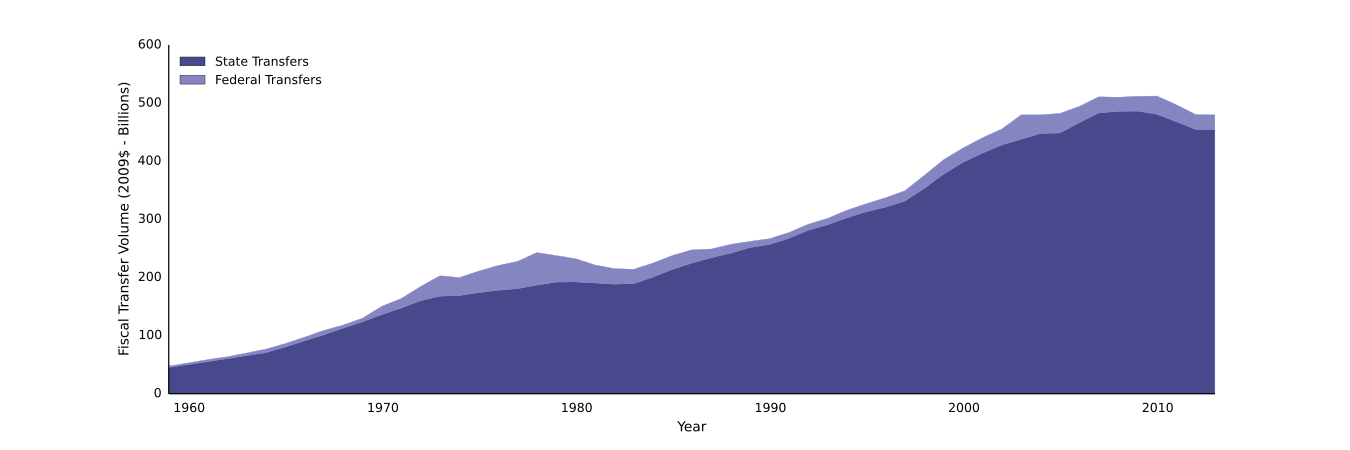
\includegraphics[width=1\textwidth]{figures/IntGov2Loc}
\end{figure}


For good cause, the intergovernmental transfer system has emerged
as a method of mitigating the intrinsic difficulties in local revenue
generation and expenditure responsibility. Local governments must
contend with mobile tax bases, and often expenditure needs that are
geographically out of phase with revenue capacity. The downside of
this development is a strong dependency by local governments on transfers
from both state and national coffers. When the economy enters a recession,
while the impacts on own source revenue may differ as a function of
revenue base disparities, a certain amount of conditional correlation
in revenue yield occurs. Not only are local fund sources depressed,
but state and national governments are far less able to provide the
same contribution via transfers. States are far more constrained given
prevailing balanced budget requirements, but national governments
can also be constrained (particularly given pre-existing debt or more
pressing political factors).


\section{Motivations for Limiting the Property Tax\label{sec:Motivations-for-Limiting-Property-Tax}}

Public opinion is of the upmost importance in a democratic country.
For the most part, the distant tails of the political distribution
have limited impact on the policies actually effected by policymakers.
However, once opinions gain critical mass, they can have large effects.
This can be particularly so when facilitated by legally sanctioned
citizen participation vehicles like ballot initiatives. Proposition
13 in California, Proposition 2$\frac{1}{2}$ in Massachusetts, and
TABOR in Colorado are likely to be the most well-known examples. Nevertheless,
statutory deviations from the property tax base have occurred as a
general phenomenon in the US.

\begin{figure}


\caption{Binding TELs in the US\label{fig:Binding-TELs}}


\begin{centering}
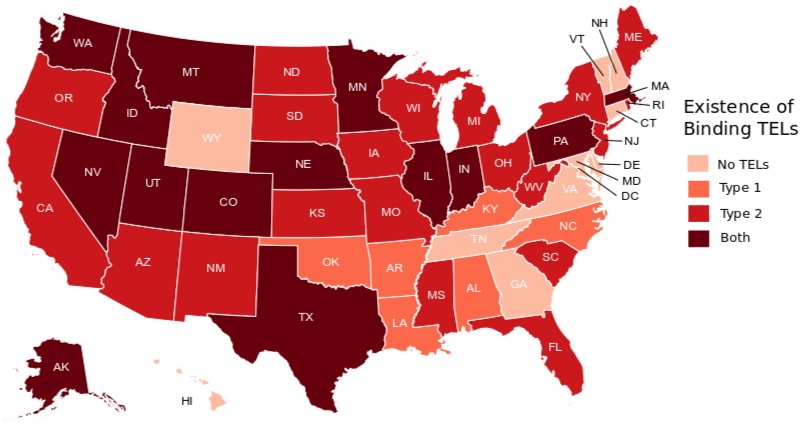
\includegraphics[width=1\textwidth]{figures/TEL_bind_states_lab}
\par\end{centering}

These data describe the variance in TEL regimes across the country.
Not all TELs bind the revenue raising capacity of local governments.
If, for example, a TEL restricts growth in assessment ratios, local
fiscal managers can still use rate increases to grow property tax
revenue. Type 1 TELs are vulnerable to circumvention, while Type 2
TELs are binding. Some states have neither, while others have both.
These data have been compiled by Daniel Mullins over a number of years.
They reflect qualified judgments about the capacity of each TEL to
bind local fiscal managers because statutory information is not a
reliable indicator.
\end{figure}



\subsection{The Argument Against the Property Tax\label{sub:Against-Property-Tax}}

The tax revolt of the 1970s was not the first effort seeking to limit
the scope of the property tax. The unpopularity of the tax has an
extensive history, including a period characterized by disdain from
both the general public and students of fiscal affairs.
\begin{quotation}
``If any tax could have been eliminated by adverse criticism, the
general property tax should have been eliminated long ago. {[}...{]}
No commission appointed to investigate any tax system, which has had
time, means, and inclination to secure the evidence, has failed to
recommend the abolition of the tax or measures tending toward fundamental
modification.''\citep{Jensen1931}
\end{quotation}
This quote captures a prevalent view among academics in the late 19th
and early 20th centuries in the US. The animosity was borne of both
seemingly intractable theoretical problems with the revenue instrument
as well as deficiencies in administration. Edward Seligman of Columbia
University constructed a multi-facted attack in his\emph{ Essays on
Taxation.}\citep{Seligman1913} In his view, there were five damning
features that made the tax ``unendurable''.


\subsubsection{Lack of Uniformity}

The tax is not actually an ad valorem tax in the sense that it is
not levied on a fixed percentage of property value. Instead, the assessment
ratio and/or tax rate are calculated in a way that takes the taxing
jurisdiction's desired total levy as a primary argument. This construct
creates the capacity for significant variation in burdens across jurisdictions,
due to the variations in fiscal requirements. The result is horizontal
inequity.


\subsubsection{Lack of Universality}

Despite numerous historical attempts to create a general purpose tax
(which Seligman discusses in some detail), the practical problem of
capturing personal property in a way that is commensurate with levies
on real property creates disparities in burden that are driven by
occupational genre rather than ability to pay or benefits received.
These practical problems are a function of both political manipulation
and the difficulty in getting a handle on intangible/administratively
inconvenient personal property.


\subsubsection{Incentive for Dishonesty}

When entire classes of property are exempt from taxation, Seligman
correctly argues that avoidance incentives are high. The rational
taxpayer will shift assets to protected classes whenever possible.
In many cases, such practices have exerted pressure on, or entirely
breached, the boundary between avoidance and evasion.


\subsubsection{Regressivity}

Seligman's context for this complaint involved his observance of the
transition away from the agrarian social context that characterized
the early period in US history. In particular, farmers were disadvantaged
in the practical taxation of property because their assets were quite
intangible and visible. In contrast, holdings derived from trade often
enjoyed tax exempted status, either de facto or de jure, as a consequence
of their intractability as administratively feasible tax handles.
Since trading wealth often exceeded that which was derived from agriculture,
this feature was a regressive one. This framework holds today in the
sense that personal property can drive a tremendous wedge in aggregate
asset holdings across homeowners. To the extent that personal property
is taxed inconsistently at best, Seligman's concerns are still valid.


\subsubsection{Double Taxation}

Property is taxed in practice based upon the value of the asset,\emph{
not the value of the property owned by the taxpayer.} Insofar as the
development of modern finance techniques has bifurcated equity stakes
in a given piece of property, the individual that physically holds
the asset is being taxed on his/her property\emph{ and the property
which is owned by the financial entity that has provided the liquidity
for the taxpayer to buy the asset.} This was perhaps Seligman's most
significant condemnation because it identified a structural phenomenon
with the potential to divorce the basis of taxation from an individual's
ability to pay.


\subsubsection{Periodicity}

Unlike the sales tax which is levied at the point of sale, and the
income tax which is largely withheld, the property tax stands out
for the timing of payments. Property tax payments are collected rarely
and are correspondingly large when collected. This creates a very
high level of visibility of property tax liability, and the economic
pain of payment is comparatively acute. From a theoretical standpoint,
\emph{this is actually a positive feature.} The nature of property
tax payment promotes transparency, as taxpayers cannot avoid thinking
about the liability. In the real world, however, it is largely this
feature that has contributed to widespread popular disdain for the
tax. This is partciularly so for taxpayers with fixed incomes that
reside in property they own.\footnote{In 2013, the Washington Post published a four-part series (\emph{Homes
for the Taking)} detailing the circumstances by which many fixed income
residents fell behind on their property taxes. In many cases, these
leins led to eviction. Such stories grow the disdain for the tax.
A more nuanced consumption of the information revealed that challenges
in administration may have been more influential than the city's property
taxation regime.} That being said, in practice, the ability to leverage escrow accounts
has attenuated the ``pain'' issue to a limited extent.


\subsection{The Argument For the Property Tax}

For all of the reasons detailed in Subsection \ref{sub:Against-Property-Tax},
the property tax endured an aggressive movement to develop other sources
of revenue. Furthermore, there were widespread statutory and constitutional
efforts to narrow the property tax base and reduce its role in financing
public expenditures in the early 20th century. These efforts were,
however, undermined by changing fiscal circumstances. The same period
saw a sharp increase in public expenditure responsibilities as a consequence
of a growing, urbanizing population and a ``lengthening of the period
of cumpulsory school attendance.''\citep{Netzer1966} In particular,
the productivity of the property tax as practiced was the source of
a new lease on life. That is, the expanding role for the state was
well-served by the reliable revenue provided by the property tax.
It should also be noted that the property tax, due to the timing of
the assessment/collection cycle, has favorable cyclical properties.
As a practical matter, local officials must be concerned with the
decline in revenue associated with economic downturns. As a consequence
of assessment lag, the property tax will typically not decline in
yield immediately (as would income and sales taxes). The delay helps
to smooth local revenue profiles and lessen the impact of macro-level
shocks.

Bolstered by the strong practical rationale for continued reliance
on the property tax, scholars have taken note of strong theoretical
arguments. As previously mentioned, the immobility of the property
tax base reduces concerns regarding the flight of the tax base from
a given jurisdiction. Furthermore, the property tax can be supported
from a benefits received perspective. While there are difficulties
coupling liability to home value, on the public consumption of services
side, the property tax can be viewed as the price of services rendered
in the jurisdiction.\citep{Oates1999} School finance, in particular,
features a significantly interdependent relationship with home values.
Home values drive the \emph{capacity} of the revenue base, but these
home values simultaneously incorporate school availability via capitalization.
From an ability to pay perspective, to the extent that home values
are at least partially correlated with incomes, the instrument does
have a progressive component to it (non-neutralities notwithstanding).
In general, despite Seligman's critique, there is a strong rationale
for the property tax's continued use.


\section{What are Fiscal Institutions?}
\begin{quotation}
``Fiscal institutions are not just there; they come into being and
develop over time. To understand more fully the workings of the public
sector, we must recognize that fiscal institutions are themselves
endogenous. {[}...{]} Moreover, since fiscal institutions are themselves
a subset of governance institutions, their evolution cannot be adequately
described or understood solely within the framework of public finance.''\citep{Oates2008}
\end{quotation}
To understand the impact of tax and expenditure limitations, it is
critical to have some idea of the other reforms that have their genesis
in the same environment. Furthermore, in setting the stage for the
institutional reforms that have beset the property tax in modern practice,
it is critical to understand the social context that permitted such
reforms to take place. As discussed in Section \ref{sec:Motivations-for-Limiting-Property-Tax},
there are theoretical underpinnings to legitimate criticism of the
property tax as a method to finance public services. These fundamental
concerns are complex and in many ways require a nuanced understanding
of taxation in general to sufficiently comprehend and design constructive
reform in practice. In the real world, however, students of public
finance are all too rare. Admiteedly, the author's bias shines through
here, but there is a kernel of truth in the sense that the motivating
factors for reform are often discordant with constructive progress.
Students of public finance need not possess any undue hubris in identifying
with Oates' observation:
\begin{quotation}
``{[}Political decisionmakers{]} sometimes design fiscal institutions
to solve political rather than efficiency problems. When fiscal solutions
have unintended effects, particularly when changes in fiscal institutions
at one level of government influence fiscal or political outcomes
at another level of government, these changes in one period generate
forces makeing for further changes in later periods.''
\end{quotation}
In this sense, Oates is making a revenue side observation that parallels
a consistent theme in the expenditure side work of Aaron Wildavsky.\citep{Wildavsky61}
To paraphrase,\emph{ a theory of public finance is a theory of politics
also.} Social dynamics and political developments are fundamental
arguments in public finance, and not simply because they have some
impact on outcomes. Political structure is the substrate upon which
public finance, as a field, is built. In subnational finance, welfare
potential is a direct result of the political institutions that govern
the capacity of the citizenry to associate, express governance opinions,
and make siting decisions. The link between welfare potential and
political structure lies in the latter serving as an input into the
cost structure of the permissible and ``prohibited'' activities
available to the citizen.\footnote{This point can be interpreted as an abstraction of the point made
by Oates: variance in local demand drives the potential for welfare
gains.\citep{Oates1999}}

Thus, while we can advance the economic critique of reform movements
and outcomes, we cannot lose sight of the fact that the economic calculations
reveal only a part of the broader tapestry of social interactions.
There is an emerging literature that has sought to shed light on this
perspective which Oates has referred to as the ``political economy
approach to fiscal federalism.'' It differs from the fiscal federalism
approach that Oates advanced in 1972, largely due to differing evaluations
of two key assumptions. First, traditional fiscal federalism assumes
that officials seek to maximize the welfare of the jurisdiction they
serve. This pursuit leads naturally to strong welfare gains as a consequence
of local variation, leading to tax-expenditure bundles that can be
better tailored to local conditions. The political economy approach
makes no such assumption, leaving room for political calculation that
may be out of phase with actual maximization of constituent welfare.\citep{Perrson_Tabellini2000,Besley_Case1995}
Second, the political economy literature does not assume, as traditional
fiscal federalism does, that central provision implies uniform public
output. Variations in output can and do arise from the legislative
process and the insertion of non-neutralities. These non-neutralities
typically arise as a consequence of the variety of political power
endowments and cultivation efforts across local jurisdictions.\citep{Seabright1996}
I would extend this further to remark that, in the context of varying
local conditions, the effect of non-neutralities is far from clear
cut. Moreover, variance in local implementation carries its own additional
source of variance in public outputs.

This view of political economy of public finaince is salient in the
current discussion because it suggests that political palatibility
is a major element in the assessment of good public financial practice.
Although the institutional reforms have limited the efficacy of the
property tax at any given point in time, these reforms may bear fruit
when assessed over time. If these reforms prolong the use of the property
tax, then a tool of fiscal autonomy - whatever its faults - has been
preserved. Indeed, the third empirical section in this study scratches
the surface on the idea of fiscal institutions as an instrument of
democracy. This is not to imply that the operational impacts of the
day are to be ignored. Some limitation of efficacy can arguably be
tolerated in the service of prolonged use\emph{ so long as the reforms
do not result in fiscal impotence.} It is thus critical to evaluate
each of the institutional reform classes that have taken a foothold
in the modern US subnational finance environment. However, in the
interests of continuity, the detailed discussion of non-TEL fiscal
institutions has been relegated to the Appendix. Only generally applicable
tax and expenditure limitations are discussed here.


\subsection{Tax and Expenditure Limitations}

Tax and expenditure limitations, or TELs, are direct attempts to limit
the growth in property tax liabilities. The vehicle for this limitation
is an explicit constraint on one of three targets: the tax rate, the
assessment base, or the entire levy. Mullins and Joyce defined six
types of limitations\citep{Joyce_Mullins1991}:
\begin{enumerate}
\item \emph{Overall Property Tax Rate Limits} set a ceiling on the property
tax rate for all jurisdictions in the state;
\item \emph{Specific Property Tax Rate Limits} set a rate ceiling for particular
types of government or different service areas;
\item \emph{Assessment Increase Limits} cap the growth rate of the assessment
base;
\item \emph{Property Tax Levy Limits} cap the growth of property tax revenue;
\item \emph{General Revenue or Expenditure Limits} cap the growth rate of
total revenues or expenditures for the state; and,
\item \emph{Full Disclosure/Truth-in-Taxation} provisions require explicit
information to be supplied to the public regarding tax changes, and
often require a specific vote to increase rates or levies.
\end{enumerate}
It is all too common for these devices to be used in tandem. A perfect
example would be California's Proposition 13, which has oft been cited
as the beginning of the most recent TEL movement.\citep{Edwards2006}
Within two years of the passage of Proposition 13, 43 states had also
implemented some kind of property tax limitation measure, 15 states
had lowered their income tax rates, and 10 states indexed their income
taxes to the rate of inflation.\citep{Sears_Citrin1985}

Admittedly, Proposition 13 was a particularly aggressive limitation
effort. It does serve, however, to demonstrate the types of impacts
that can occur with these reforms. Such effects do not occur everywhere,
particularly when reforms are not of the binding variety defined by
Mullins and Joyce. Binding limitations provide no workaround to achieve
the same revenue targets. A two-part composite reform created this
environment in California. Passed on June 2, 1978, Proposition 13
limited assessment increases to 2\% annually and mandated a rate ceiling
of 1\%. Rather than address the revenue yield directly, voters chose
to limit the base and rate inputs. Furthermore, assessed values reverted
back to 1976 levels. Couple this reduction in the base with the practice
of acquisition value assessement, in which real estate values only
reflect the market value at the time of sale, and one gets a potent
mix for revenue reduction.
\begin{quotation}
``The effect was dramatic. Property tax revenue immediately fell
by 57 percent across the state. Local governments in California collected
over \$6.6 billion less in property tax revenue in 1979 than they
did in 1978 (Citrin 1984). California property taxes went from 51
percent above the national average in 1978 to 22 percent below the
average in 1981.''\citep{Yuan_Cordes_Brunori_Bell2009}
\end{quotation}
The stringency, scope, and type of limitations vary across states,
and in turn, so do the impacts of these reforms. Many observers, however,
have noted some common themes. TELs appear to be related to a reduction
in educational services output. Figlio and Rueben find that the quality
of teachers produced, as measured by the relative test scores of education
majors, is lower in TEL states.\citep{Figlio_Rueben2001} Downes et
al. find limited evidence of poorer student performance in TEL districts,
but caution that 1) the variation in impact suggests that only some
districts are adversely impacted and 2) the impacts of TEL implementation
have not yet forced dramatic cuts to education.\citep{Downes_Dye_McGuire1998}
Downes and Figlio has more to say on this front, noting that local
governments impacted by TELs tended to feature lower math testing
scores from students.\citep{Downes_Figlio1999}

TELs have been defended as grassrotts efforts, but the ironic reality
is that they often adversely affect local autonomy. Mullins \& Joyce\citep{Joyce_Mullins1991}
and Edwards\citep{Edwards2006} have observed that TELs encourage
greater reliance on non-tax revenue, but this source has been insufficient
to cover the gap. The consequence is greater reliance on state funding
for local services.\citep{Sokolow1998,Sokolow2000} The increased
reliance has resulted in an upward shift in the locus of authority
for local services, and a proliferation of special districts at the
local level.

While Colorado's TEL regime is not quite as extreme as California's,
it still features overlapping policies. In particular, there is the
SLPTR, TABOR, and the Gallagher Amendment. The impact of these policies
is the focus of this study, and their characteristics will be explored
in detail in Section \ref{sec:COTELs}.


\section{Do TELs Alter Local Fiscal Behavior?}

In their study of Proposition 2$\frac{1}{2}$ in Massachusetts, Cutler,
Elmendorf, and Zeckhauser\citep{cutler1999restraining} noted that
``{[}c{]}itizens have increasingly resorted to referenda when they
do not trust their elected officials to serve their interests.''
The situation appears to be a classic agency problem\footnote{It is important to note that Cutler, Elmendorf, and Zeckhauser examine
a range of theoretical models of behavior.}, insofar as constituents often have insufficient information to evaluate
the implications of changes in local fiscal policy. The same study
references survey data related to Proposition 2$\frac{1}{2}$.\citep{ladd1982voters}
The data suggest that voters largely did not want to change the basket
of local services they enjoyed prior to its passage. Cutler et al.
found empirical support for very different motivations:
\begin{itemize}
\item Due to the difficulty in closely monitoring government activity, voters
assumed waste must exist.
\item Voters believed waste was rampant, but came to regret the cuts associated
with Proposition 2$\frac{1}{2}$.
\item Voters believed their property taxes were too high, irrespective of
their satisfaction with current service levels.
\end{itemize}
In general, the sentiment seemed to suggest a widespread belief that
taxes could be limited without substantial implications for fiscal
operations. In reality, the literature suggests that TELs have very
real impacts on local revenue and expenditure behavior.


\subsection{Revenue Implications}

TELs are often motivated by dissatisfaction with the property tax.
Alm and Skidmore\citep{alm1999tax} find that states with increasing
levels of property taxation and/or increasing ratios of local to state
revenue are more likely to pass TELs. The focus on the property tax
may be a consequence of the visibility of associated tax prices, another
significant predictor of TEL passage. To this end, TELs have been
quite productive in reducing the growth in property tax revenue\citep{shadbegian1998tax,rown2000constitutional,Dye_McGuire1997}
and tax revenue generally.\citep{shadbegian1999effect,mullins1996tax,skidmore1999tax}
Ballal and Rubenstein conducted a meta-analysis of the literature,
and concluded that more recent studies are in strong agreement about
the depressing impact of TELs, in contrast to the older literature.\citep{ballal2009effect}
They posit that this shift is likely due to either better measurement
techniques, or constraints that are increasingly binding over time.
This study finds support for both explanations. Accounting for spatial
dependency across counties in Colorado does alter the depressive impact
of TELs on local revenues. Furthermore, TELs in Colorado have a dynamic,
cumulative effect due to the ratcheting property of TABOR.

The impact on resources for local service delivery is a more complicated
matter. The reductions in tax revenue are partially offset by a shift
in the local revenue portfolio. TEL-constrained local governments
are more likely to increase reliance on miscellaneous revenue, fees,
and charges.\citep{mullins1996tax,shadbegian1999effect} Such a shift
does promote a benefit-based finance structure, insofar as constituents
are increasingly asked to directly incur the marginal cost of service
provision. There are also, however, distributional implications. Although
it is less of a concern at the state and local level, fees and charges
are generally more regressive than broad-based taxation that may be
tied to indicators of income. Local governments are also limited in
their ability to completely offset the loss in tax revenue. The more
stringent the TEL, the more difficult the offset becomes.\citep{shadbegian1999effect}

To help address the shortfall, TEL-constrained local governments are
increasingly reliant on state transfers.\citep{mullins1996tax,skidmore1999tax}
Such a shift implies a reduction in local autonomy, which has implications
for the ability of local officials to respond to the preferences of
constituents. To the extent that local officials can negotiate with
state officials instead of ask constituents to raise more revenue,
the link between local preferences and local service delivery is weakened.
Direct connection between own-source revenue and services rendered
promotes better assessment of the opportunity costs associated with
local policies. That being said, the extent of this offset is limited
when TELs operate on both state and local governments\citep{Joyce_Mullins1991},
which is the case with TABOR in Colorado. In these cases, states are
more reluctant to provide enough aid to fill the void.

It should also be noted that TELs impose constraints that vary widely
across jurisdictions.\citep{bradbury2001property,rown2000constitutional}
In particular, they are more constraining on urban jurisdictions,
which have greater numbers of disadvantaged constituents.\citep{Mullins2004}
Thus, the imposition of TELs raises important questions related to
equity. Indeed, it is this differential impact that serves as the
motivational basis for this study.


\subsection{Expenditure Implications}

While it has been shown that TELs and related policies are associated
with declines in local spending generally\citep{shadbegian1998tax,bails2000impact,feld2003budget},
most studies have focused on implications for the dominant service
delivered at the local level: education. Educational resources are
increasingly coming from the state level.\citep{shadbegian2003did,ballal2009effect}
In Michigan, for example, the state proportion of K-12 education funding
jumped from 30\% to 70\% between 1993 and 1995, once local approval
for tax increases was required.\citep{Sokolow1998}

Variance in implications for local service delivery is heavily dependent
upon macroeconomic conditions. In their review of Proposition 2$\frac{1}{2}$,
Cutler et al. found that the impacts of the TEL were smaller than
anticipated during the 1980s. The intended reduction in local revenue
collection was offset by an increase in the tax base from new construction,
and increased state aid to municipal governments. However, when a
recession hit in the early 1990s, new construction slowed and the
state was less willing to provide offsetting transfers. The impact
of Proposition 2$\frac{1}{2}$ became much more pronounced. Indeed,
the strength of the policy in general has been explicitly weakened
with amendments. One such amendment increased the levy limit to account
for new construction. Another permitted local voters to choose to
collect more revenue. In Colorado, TABOR features both of these innovations.

Bradbury, Mayer, and Case also studied Proposition 2$\frac{1}{2}$.\citep{bradbury2001property}
They found that communities constrained by the limit were unable to
finance increases in school expenditures. Moreover, they showed that
school expenditures were capitalized into the home prices within a
given community. Communities that could not match these increases
experienced adverse impacts on the value of their housing stock. Thus,
in addition to the equity concerns associated with the differential
impact of TELs across communities, there are downstream effects that
may exacerbate preexisting inequity.

\clearpage


\chapter{Fiscal Behavior in Colorado\protect\footnote{For long-term price changes, this analysis uses the Chained Personal
Consumer Expenditures Index. The primary reason is that the PCE, in
contrast to the Consumer Price Index, accounts for changes in the
basket of consumed goods over time and substitution for less expensive
alternatives when the price of a particular good increases.\citep{FOMC2000}}\label{chap:CO-FiscBehavior}}

As of June 30th, 2012, Colorado contained the 11th highest count of
governmental entities in the nation: 2,905.\citep{Census_COG2013}
As previously mentioned, there were 62 counties in the state, and
two city-county governments: Broomfield and Denver. There were also
271 cities and towns of the general purpose variety, and no townships.\footnote{These tallies include Broomfield and Denver in the municipal government
count, in order to correspond to Census figures.} On the specialized jurisdiction side, there were 180 school districts
and 2,392 special districts. While this analysis focuses on counties
entirely, it is important to recognize the complexity of the jurisdictional
structure.

Footnote: For long-term price changes, it is desirable to use the
Chained Personal Consumer Expenditures Index. The primary reason is
that the PCE, in contrast to the Consumer Price Index, accounts for
changes in the basket of consumed goods over time and substitution
for less expensive alternatives when the price of a particular good
increases.\citep{FOMC2000}


\section{Which Socioeconomic Dynamics Characterize the Study Period (1993-2009)?}

As can be seen in Figure\ref{fig:Colorado-GSP}, although economic
growth clearly stagnated during national recession periods, the Colorado
economy grew dramatically in real terms over the study period. Between
1993 and 2009, the real gross state product grew over 90\%. Nevertheless,
the recessionary periods had outsized influence. Insofar as revenues
declined in those years, the baseline against which future revenues
were to be compared was reduced. The ``ratcheting'' implications
of this process will be discussed further when the TEL policies are
presented in more detail.

\begin{figure}
\caption[CO GSP]{Colorado's Real Gross State Product (1963-2013)\label{fig:Colorado-GSP}}


\centering{}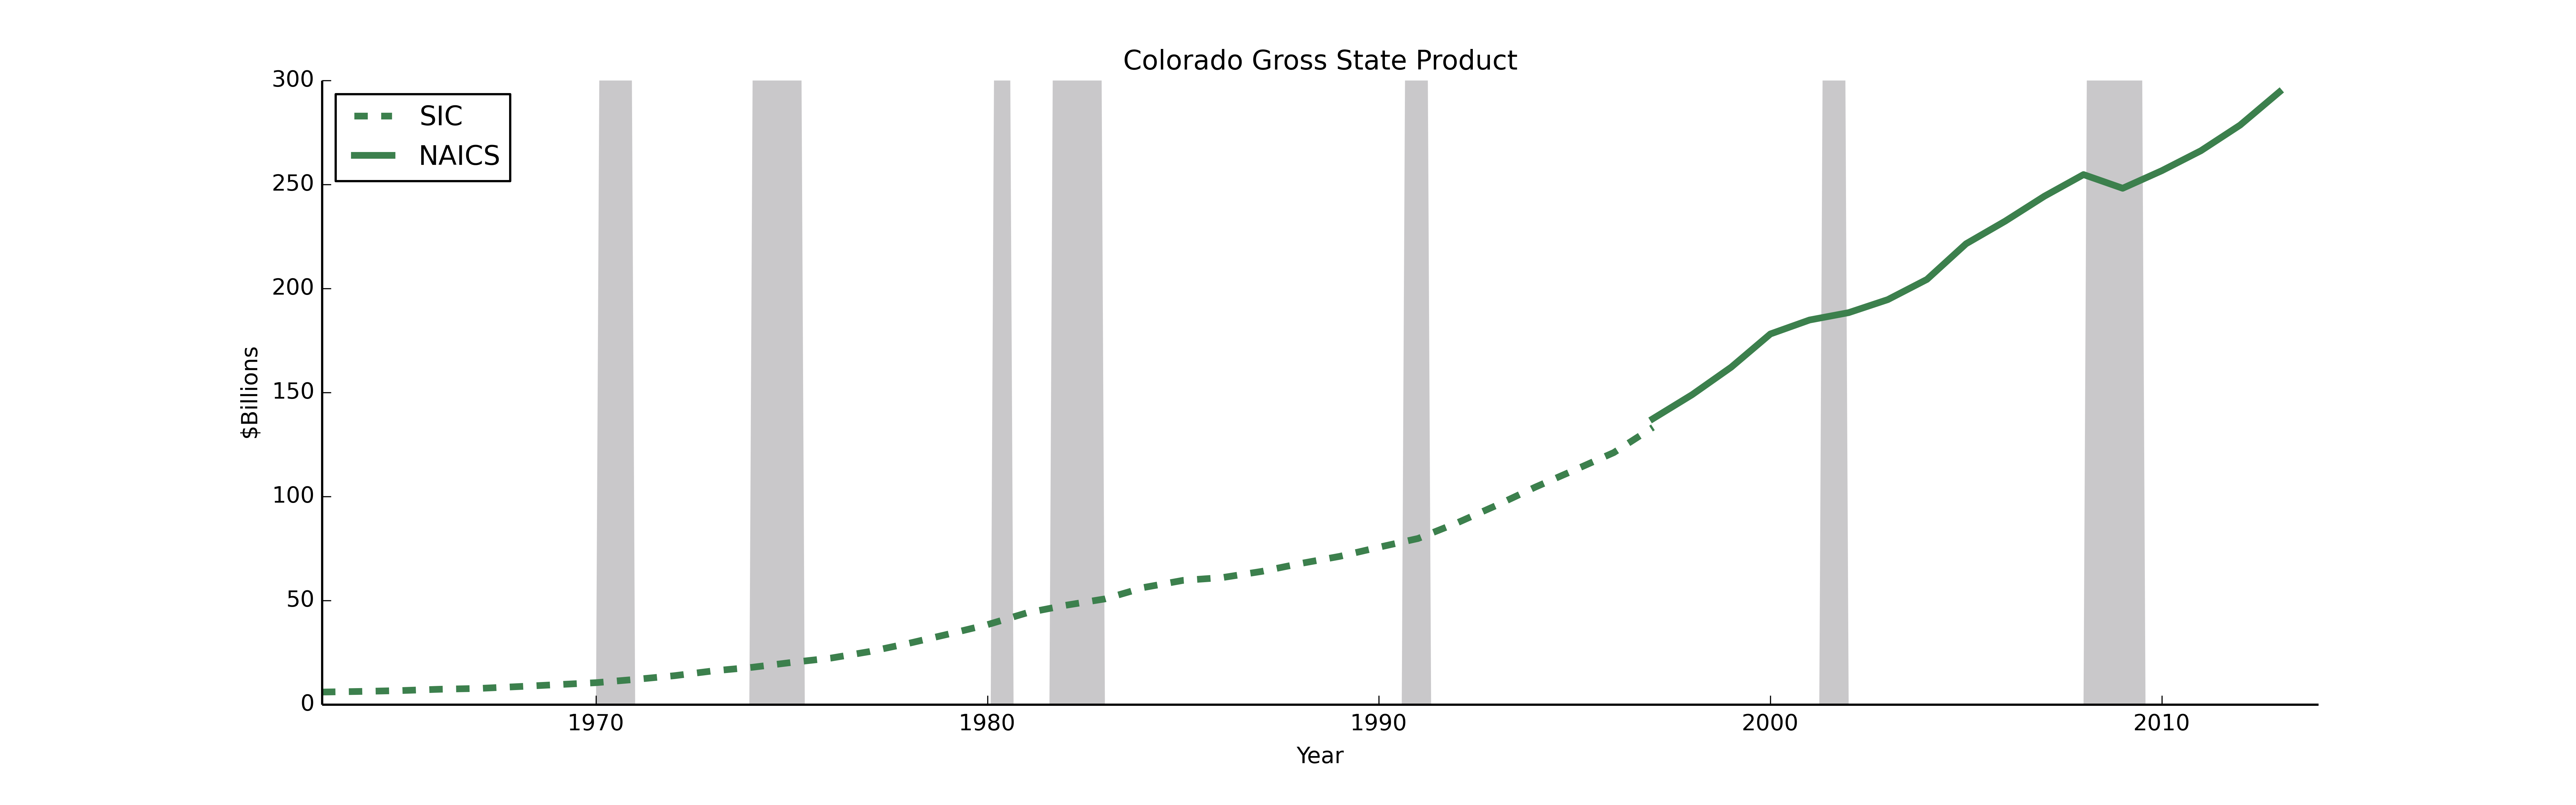
\includegraphics[width=1\textwidth]{figures/CO_gsp}
\end{figure}


Over the 1975-2009 time period, according to demographic information
acquired directly from the Colorado Division of Local Affairs, the
population across all counties grew 93.4\% (2,589,171 to 5,008,427).
Figure \ref{fig:County-Population-Dynamics} displays total population
growth and the distribution of county population by year via violin
plots.\footnote{Violin plots are essentially richer versions of box plots. The median
value is given by the``heavy'' dashed line, while the first and
third quartile values are given by the``light'' dashed lines. The
sides of each``violin'' are actually mirror images of the kernel
density estimate. Thus, wide portions indicate regions in which many
observations lie, while narrow portions indicate a relative paucity
of observations.} While the population has grown notably over time, the violin plots
indicate that a relatively small portion of this growth is due to
increases in the median county population. Rather, most of this growth
is due to an increase in the size of the largest counties.

\begin{figure}


\caption[County Population]{County Population Dynamics Over Time\label{fig:County-Population-Dynamics}}


\begin{centering}
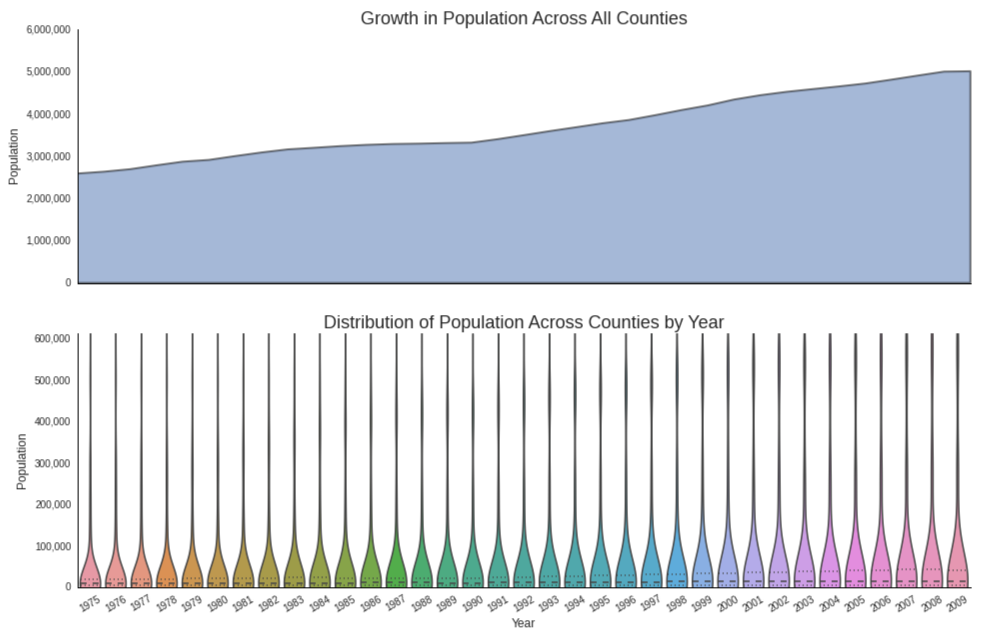
\includegraphics[width=1\textwidth]{figures/CO_pop_growth}
\par\end{centering}

Fix axis labels
\end{figure}


With respect to the tax base, as expected, the number of housing units
scales tightly with population. Interestingly enough, however, the
highest value housing tends to reside in the comparatively smaller
counties. Home values do not scale tightly with population, which
may suggest that the desire for land scales with income. Most counties
contain less than 100,000 people, further supporting the notion that
outlier counties are driving the population growth. The distribution
of housing stock value is characterized by a high level of variance,
which is highlighted in the second panel of the plot. As may be expected,
the income base also exhibits a great deal of variation. Figure\ref{fig:Distribution-of-Income}\footnote{Blue indicates higher values while red indicates lower values.}
demonstrates that this variation in magnitude has a strong spatial
contigent as well. Wealther counties reside disproportionately in
the northern and northwestern portions of the state. Median houshold
incomes range from \$25,309 to \$101,108.

\begin{figure}


\caption[Distribution of Income]{Distribution of Income\label{fig:Distribution-of-Income}}


\centering{}\includegraphics[width=1\textwidth]{figures/CO_med_inc_cty_map}
\end{figure}


As we will see, this spatial variation and apparent spatial clustering
plays a role in parsing the impact of TELs in the state.\footnote{Although the data are collected from the 5-year ACS over the 2008-2012
period, they can be loosely interpreted as a point in time.} Unemployment and poverty rates exhibit wide variation. Unemployment
rates varied from 2.4\% to 20.1\% during the survey period (2008-2012),
while poverty rates varied from 3.9\% to 22.5\%. The inverse relationshp
between median household income and measures of economic stress is
material.


\section{Which Revenue Sources are Employed?}

In 2011, the Census Bureau estimates that local governments in Colorado
raised \$29.7 billion in revenue from all sources. Tax revenue, the
source most directly affected by TELs, amounted to \$12.3 billion.
The largest single source of tax revenue was the property tax. Local
governments collected over \$8 billion in property tax revenue, approximately
67.5\% of tax revenue and 28.0\% of total revenue. Sales and gross
receipts revenue, the next largest source of own-source revenue, accounted
for \$3.3 billion.

In real terms, Colorado experienced consistent growth over the 1975-2009
time period. Overall, county revenue increased by 72\% over the period
on average (from \$1,013 to \$1,741). These measures of central tendency,
however, mask considerable variation in the individual trajectories
of specific counties. The average range of per capita revenue was
\$3,772 over the same period. Note also that the median revenue per
capita increase (63\%) did not significantly lag the mean increase,
suggesting a relatively stable distribution of county revenue across
time.

\begin{figure}
\caption[County Revenue]{County Revenue Growth\label{fig:County-Revenue-Growth}}


\centering{}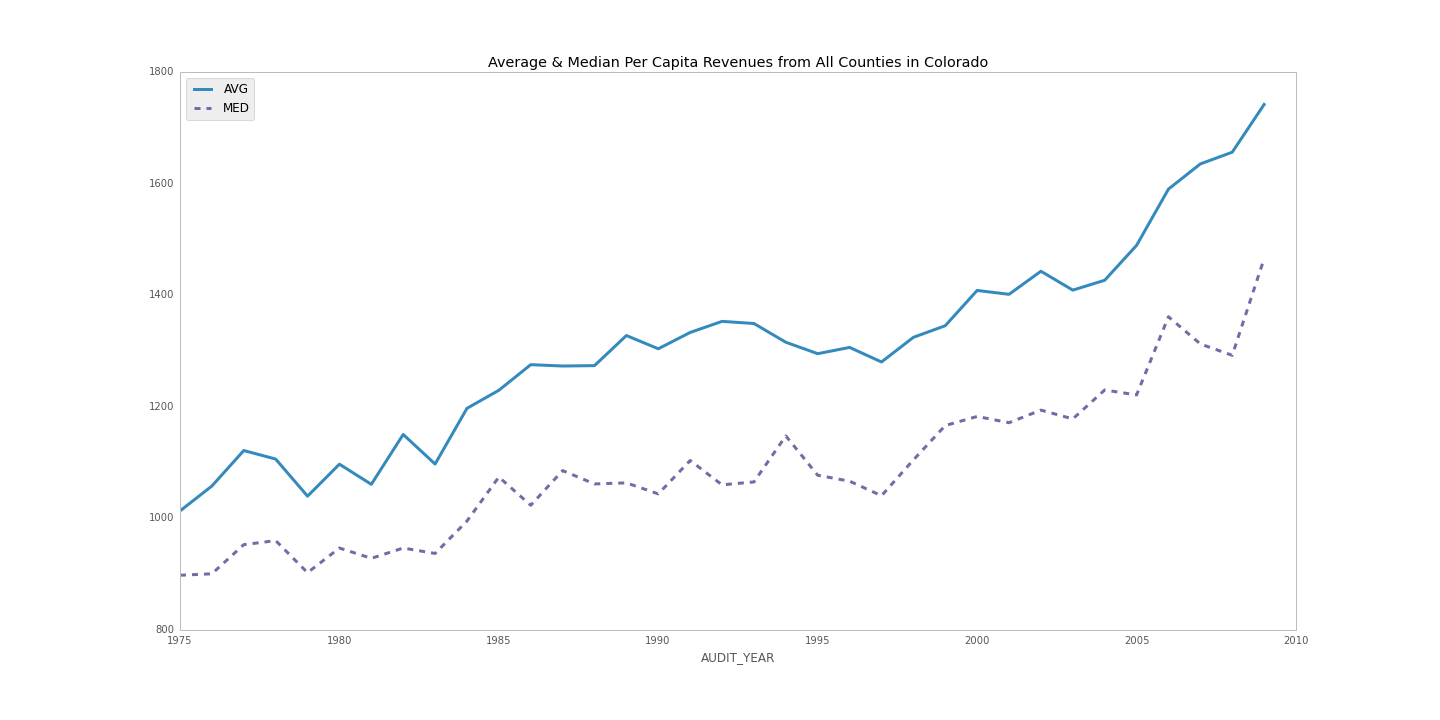
\includegraphics[width=1\textwidth]{figures/CTY_rev_growth}
\end{figure}


Somewhat surprisingly, the growth in tax receipts (+187\%) over the
period outpaced growth in intergovernmental transfers (+42\%). As
Mullins and Joyce have noted, there has been a general increase in
local dependency on higher level transfers in addition to dependency
on fees and charges associated with the imposition of strong TELs.\citep{Joyce_Mullins1991}
In fairness, however, the target of these TELs is usually the property
tax. While the property tax has grown in terms of receipts (+168\%),
it has fallen as a percentage of total tax revenue (-6.5\%). Moreover,
the growth in sales revenue as a percentage of all tax revenues has
increased dramatically (+30\%). It has also stood out as the fastest
growing revenue source (+273\%). Although it remains a small portion
of the overall portfolio, license revenue grew faster than all other
sources (+489\%), followed by revenue from charges (+406\%). This
growth is consistent with the expected impacts of TEL policies.

\begin{figure}


\caption[Revenue Composition]{Revenue Composition\label{fig:Revenue-Composition}}


\centering{}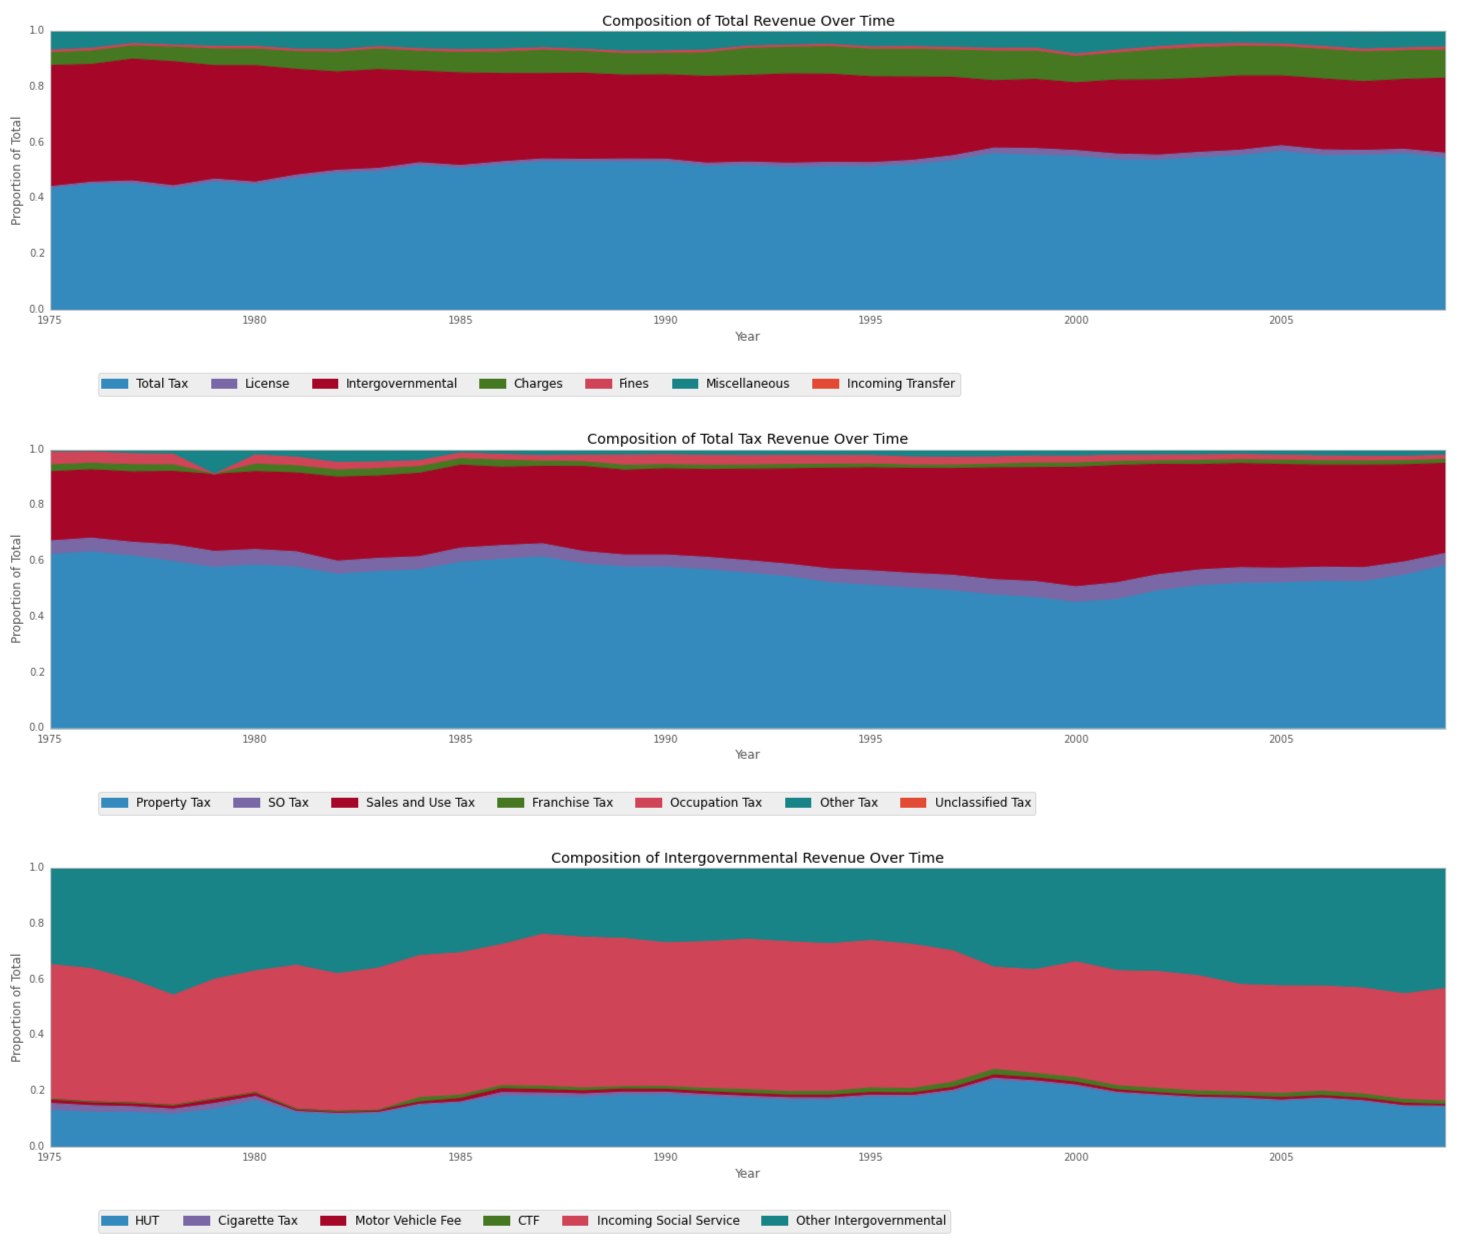
\includegraphics[width=1\textwidth]{figures/CO_cty_rev_comp}
\end{figure}



\section{Which Expenditure Responsibilities Exist?}

On the expenditure side, local governments spent \$29.5 billion in
2011. Virtually all expenses were direct expenditures (99.8\%). As
is typically the case, the single largest line item was elementary
and secondary education, amounting to \$8.1 billion (27.7\% of total
expenditures). At \$4.2 billion and \$4.0 billion, environment/housing
and public safety are the next two dominant functions from a budgetary
perspective.

\begin{figure}


\caption[County and Municipal Finances]{Summary of County and Municipal Finances in Colorado\label{fig:cty-muni-fin-summary}}


\begin{centering}
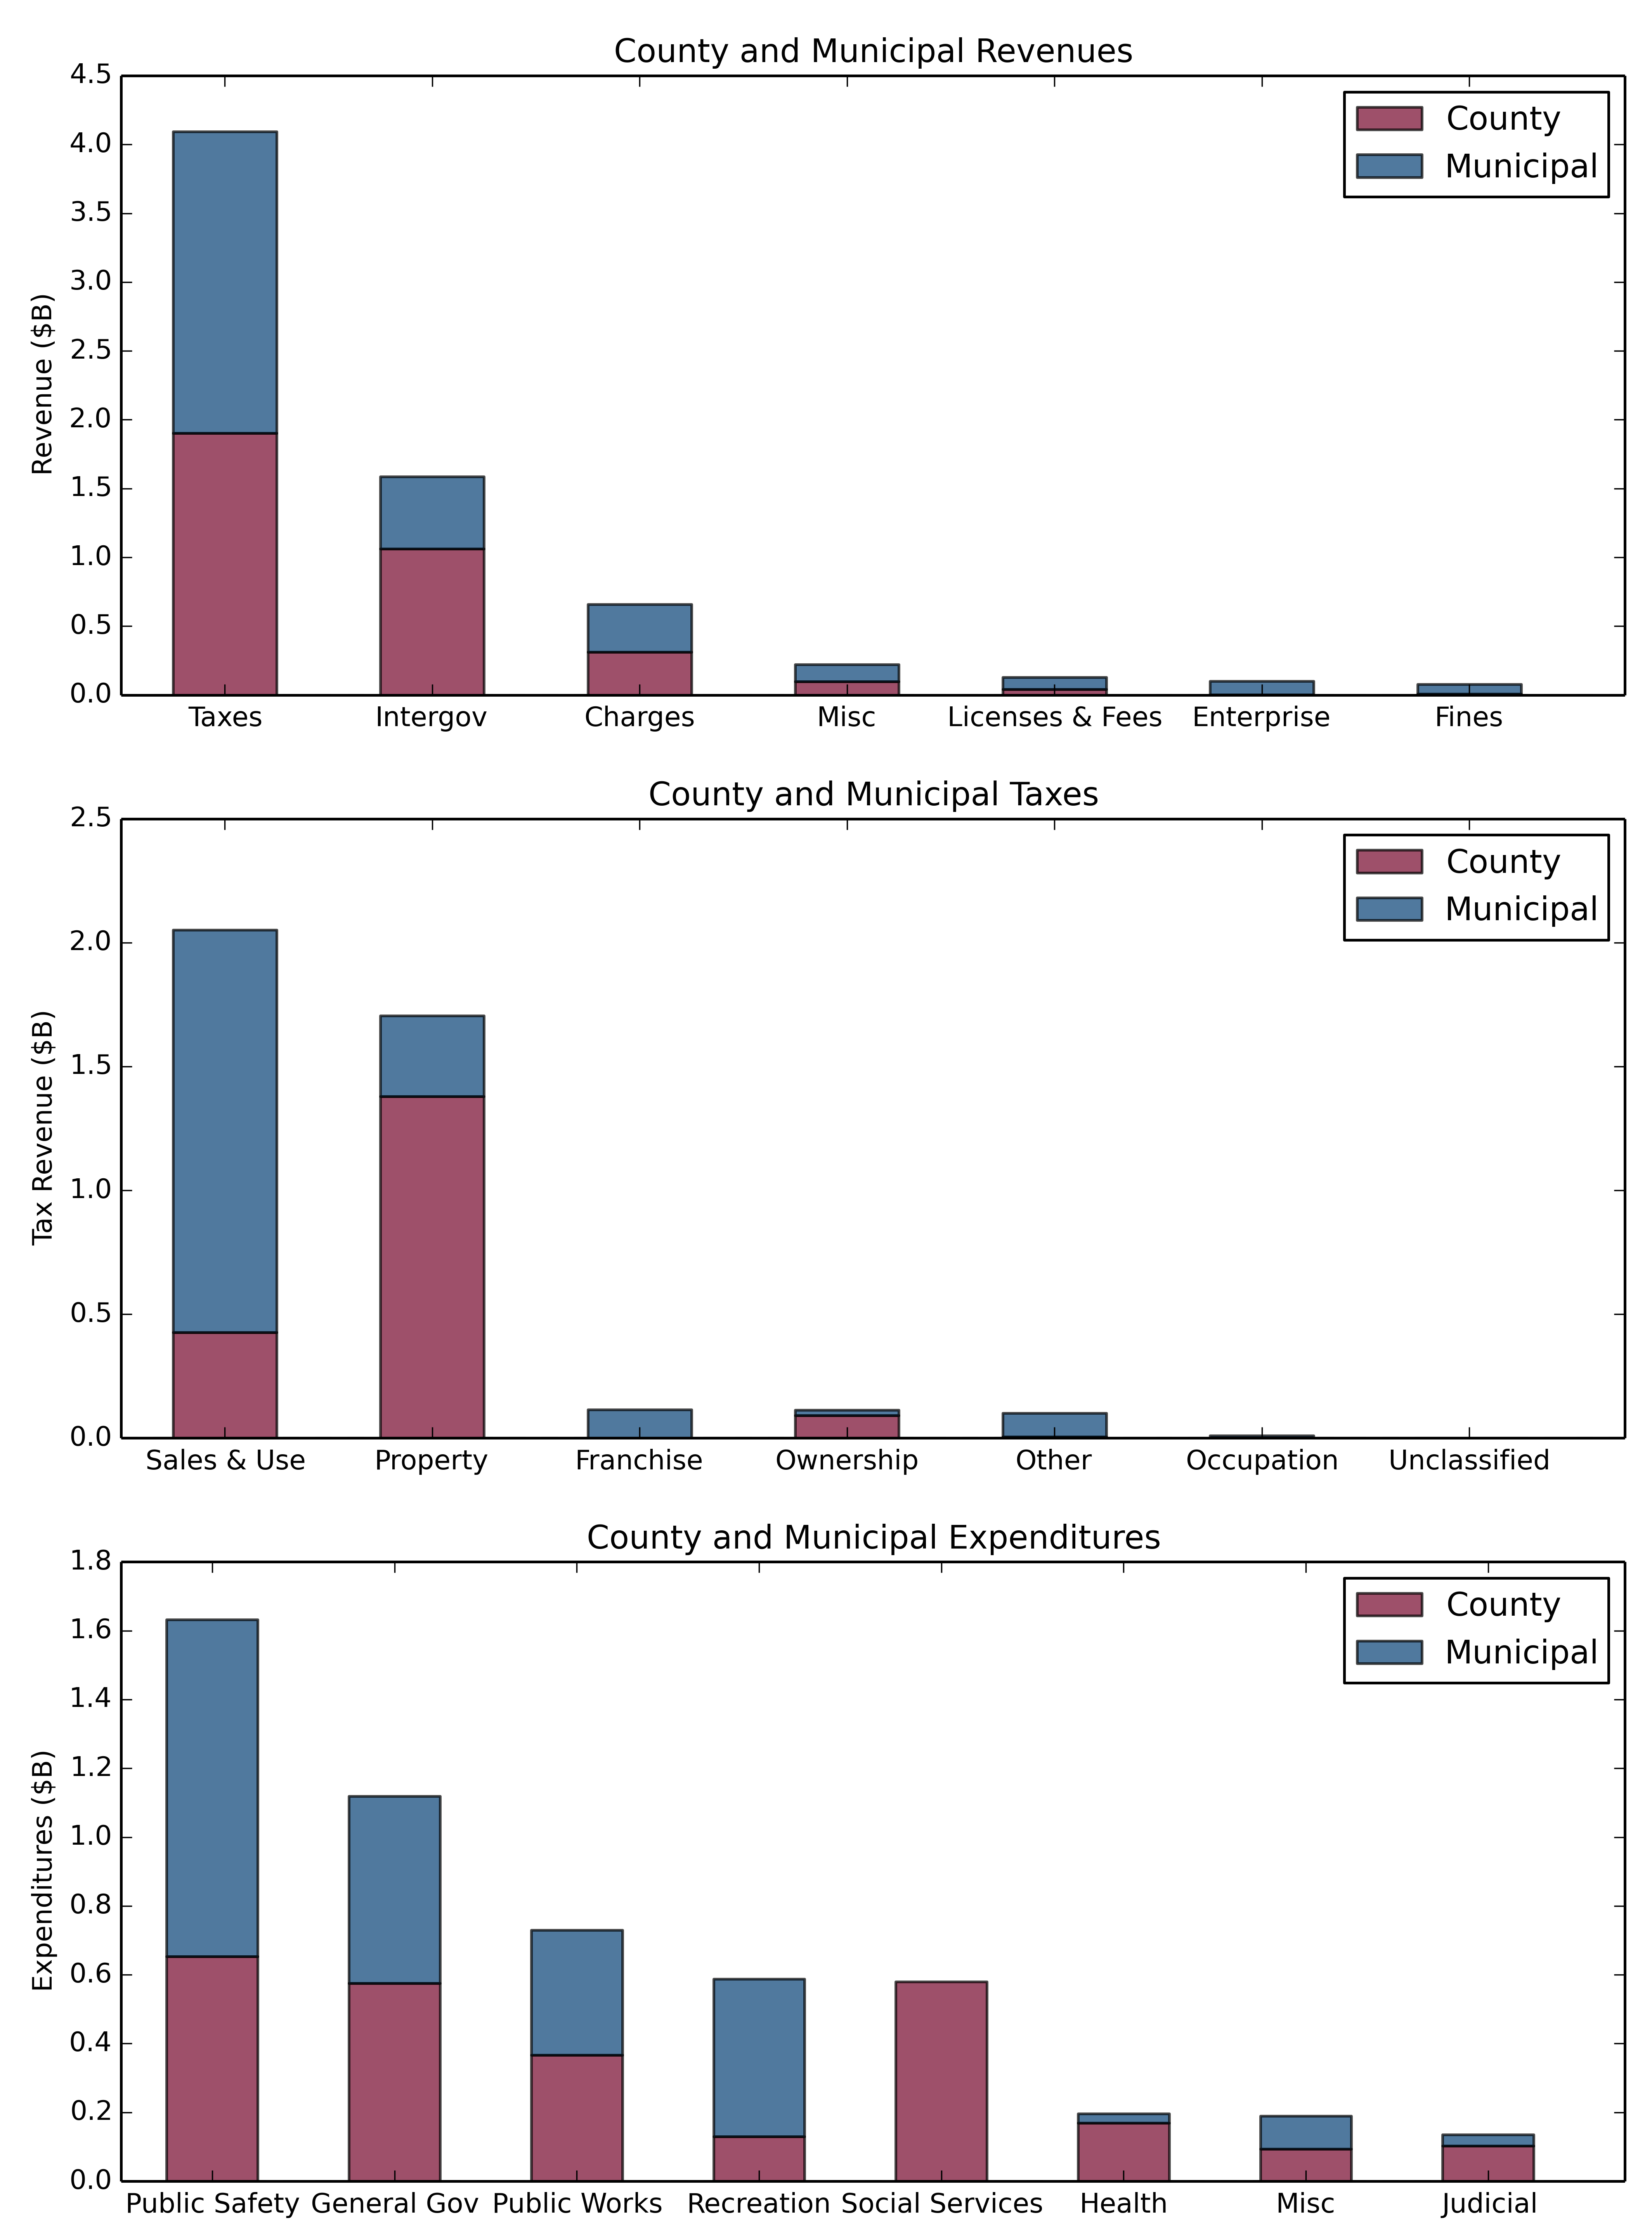
\includegraphics[width=1\textwidth]{figures/cty_muni_fin_summary}
\par\end{centering}

The Colorado Division of Local Affairs provides 2010 fiscal data for
counties and municipalities. Relative to the Census data, these data
permit a more nuanced view of the functions served by general purpose
jurisdictions in the state. There are three particularly noteworthy
insights revealed by the data. First, property taxes are the revenue
source most directly impacted by TELs, and they are predominately
levied by county level governments. Second, taxes in general are far
and away the dominant sources of revenue for general purpose jurisdictions.
Third, counties play a major role in the direct delivery of services.
All three of these facts suggest that policies that impact the property
tax, in particular, have substantial potential to directly affect
the public services consumed by Colorado residents.
\end{figure}


both growth in average (+65\%) and median (+61\%) liabilities per
capita has remarkably lagged growth in revenues over the 1975-2009
period (Figure\ref{fig:County-Expenditure-Growth}). As with the revenue
trajectories, median expenditures mirror average expenditure growth
rather closely.

\begin{figure}


\caption[County Expenditures]{Real County Expenditure Growth\label{fig:County-Expenditure-Growth}}


\centering{}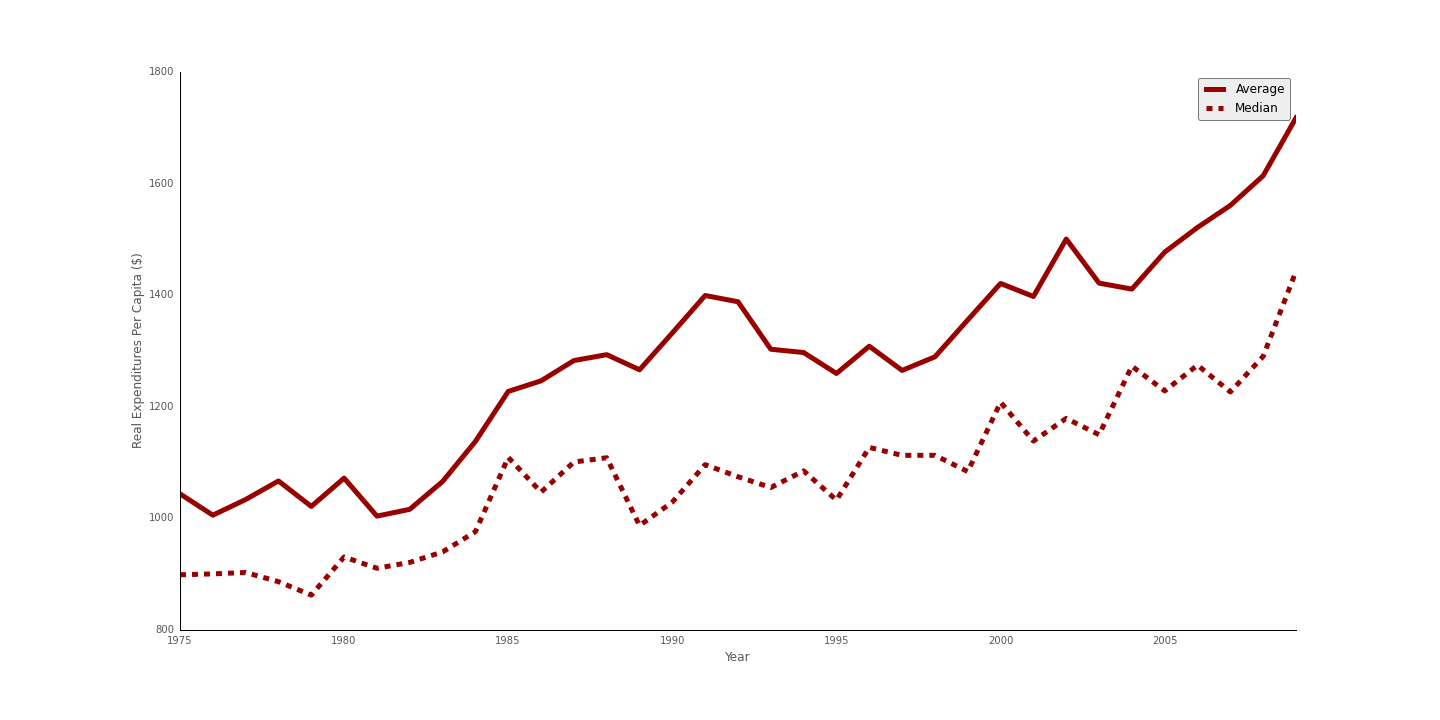
\includegraphics[width=1\textwidth]{figures/CTY_exp_growth}
\end{figure}


While debt service has been the fastest growing liability for counties
in Colorado (+633\%), it still remains a small portion of the overall
budget (4.7\% in 2009). The dominant liability resides with operating
expenditures. Given the preponderence of direct spending activity
at the local level, this is unsurprising. Operating expenditures increased
116\% over the period, but fell as a percentage of total expenditures
(79\% to 76\%). Within operating expenditures, the fastest growing
line item was judicial expenditure (+263\%), although it constituted
only 3.6\% of operating expenditures in 2009. The real story is in
public safety, which grew 231\% over the period. This spending increased
its compositional importance notably, growing from 19\% to 29\% of
operating expenditures and 15\% to 22\% of total expenditures.

\begin{figure}


\caption[Expenditure Composition]{Expenditure Composition\label{fig:Expenditure-Composition}}


\centering{}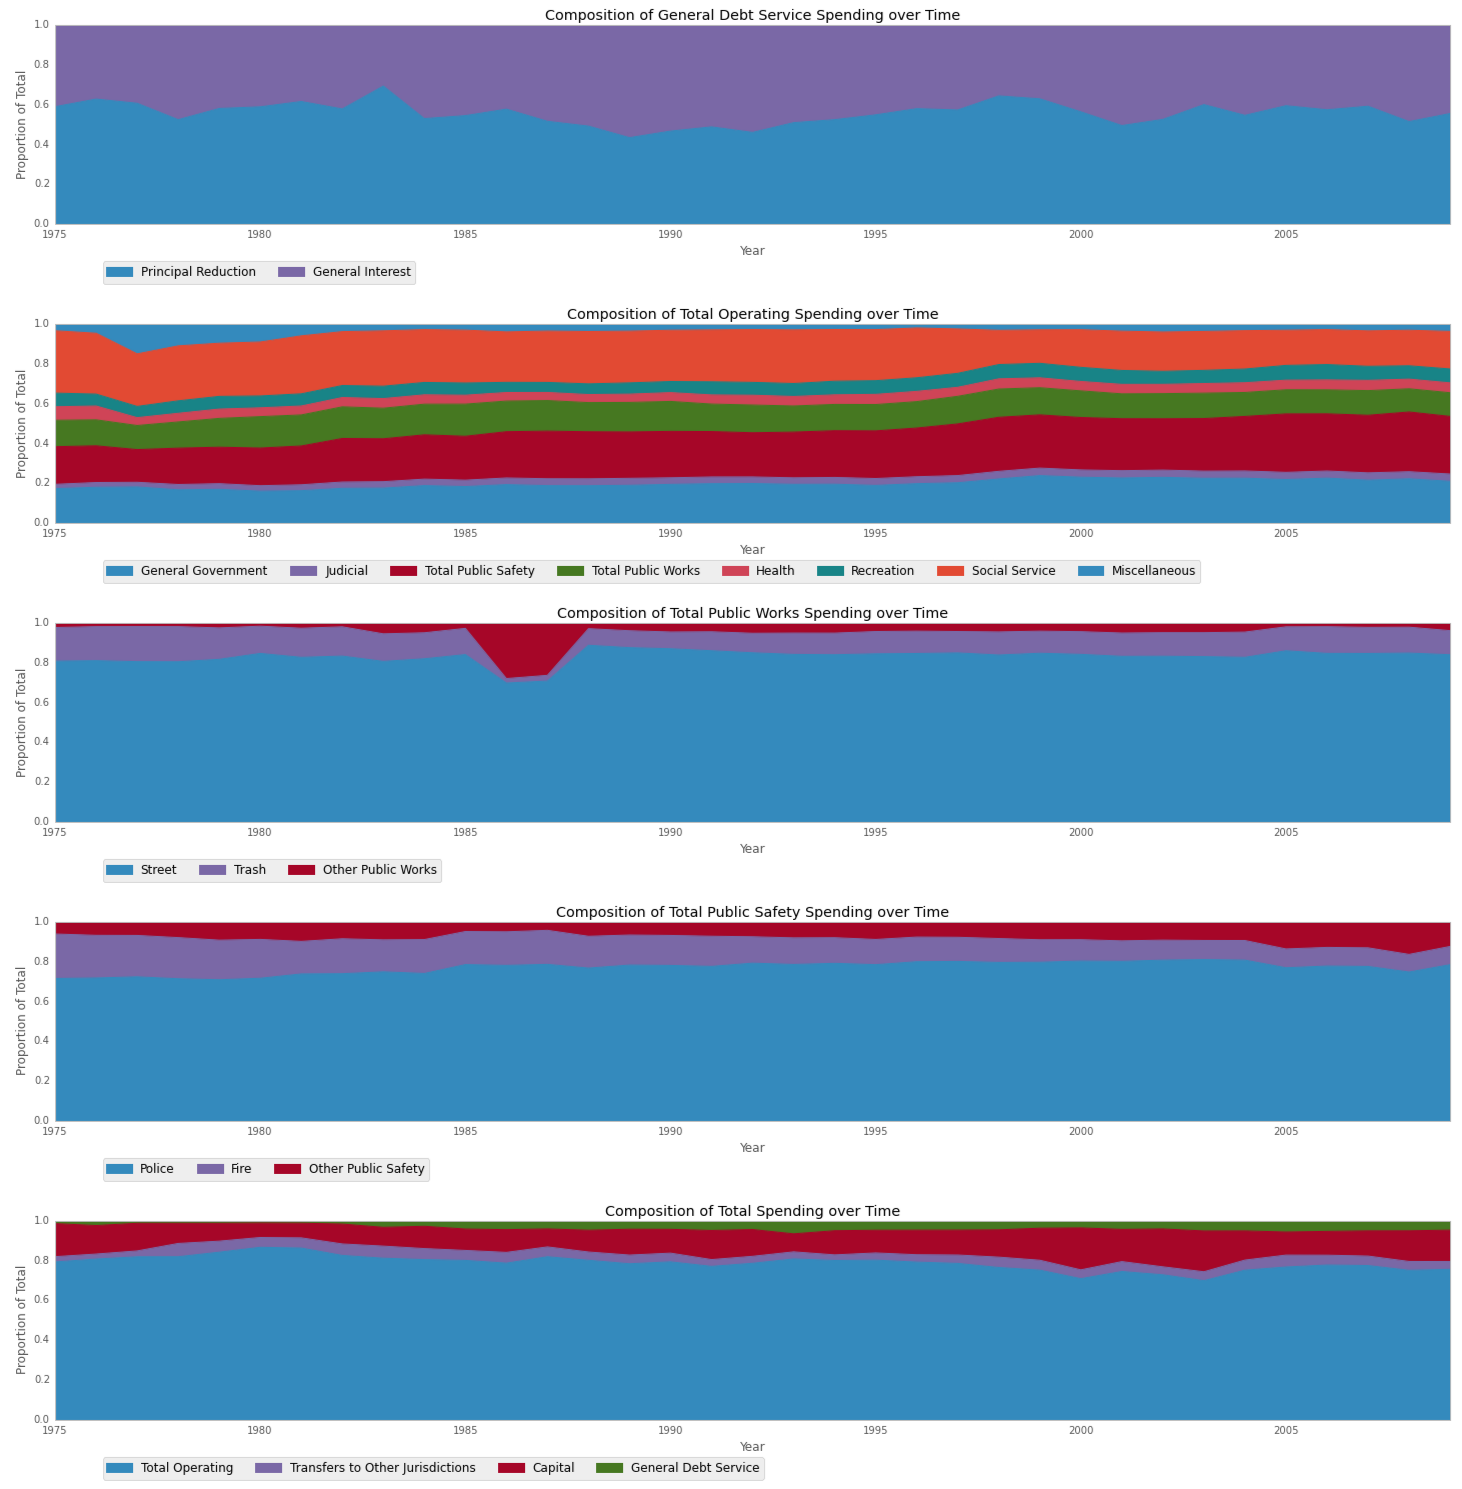
\includegraphics[width=1\textwidth]{figures/CO_cty_exp_comp}
\end{figure}



\section{What is the TEL Landscape in Colorado?\label{sec:COTELs}}

As noted in the beginning of this study, the TABOR amendment was passed
in 1992. TABOR is by far the most well known of the Colorado TELs,
but in fact, the history of TELs in Colorado started much earlier.
What follows is a timeline of major TEL initiatives in Colorado:
\begin{itemize}
\item 1913: Colorado General Assembly approves a measure limiting the annual
growth in state-level property taxes to 15\%.\footnote{The state property tax was eliminated in 1964.}
\item 1964: The state property tax was abandoned, but limits on local property
tax revenue growth were set to 5\% annually.
\item 1976: Statewide limitations on local property tax growth were increased
from 5\% to 7\% (this refers to the Statewide Limit on Property Tax
Revenue).
\item 1977: The``Kadlecek Amendment'' limited annual growth in state General
Fund Appropriations to 7\%, and required the maintenance of a 4\%
reserve.
\item 1979: The Kadlecek Amendment was made permanent.
\item 1982: The Gallagher Amendment was passed, limiting the allowable assessment
value of residential property.
\item 1984: The Kadlecek Amendment increased the limit to 7\%, plus the
costs of property tax reappraisals.
\item 1988: The SLPTR was decreased to 5.5\%.
\item 1991: The statutory state-level General Fund appropriation limit (a.k.a
the Arveshoug-Bird Limit or ABL) caps growth at the lesser of either
5\% of growth in statewide income, or 6\% growth over the previous
year's appropriation level.
\end{itemize}
While multiple limits act at the state level, our focus for this analysis
is local revenue behavior. In particular, we are concerned with the
property tax, which has stood out over time as the most important
revenue source for local governments. For this reason, we will further
unpack the three most significant reforms in this areas a bit further:
TABOR, SLPTR, and GA.


\subsection{Taxpayer's Bill of Rights}

TABOR is, in and of itself, a composite measure that acts on individual
tax districts. Tax districts in this case represent local jurisdictions
that raise revenue, such as general purposes municipalities, counties,
and school districts. It features three major elements that work in
concert to limit revenue growth: voter approval for tax increases,
a limitation on the growth in revenue, and protection of the existing
limits.

For the purposes of TABOR, a tax increase is defined as any one of
the following:
\begin{itemize}
\item New tax instrument;
\item Tax rate increase;
\item Local mill levy increase;
\item Property assessment valuation ratio increase;
\item Extension of an expiring tax; or,
\item Any tax policy resulting in a net tax revenue gain.
\end{itemize}
If any of the above are proposed, they must be validated by explicit
voter approval in the jurisdiction in question. On the other side,
no voter approval is required for a tax decrease. Note, however, that
such a decrease resets the baseline to a new, lower level. This is
one manifestation of the so-called ``ratchet effect'' which will
be explored further below. TABOR also explicitly prohibits some types
of new taxes.\footnote{Prohibited taxes include new or increased real estate transfers, local
income taxes, state property taxes, and surcharges on state income
taxes.}

The limit on annual revenue growth for a tax district is set by formula,
which generally accounts for increases in inflation\footnote{The Consumer Price Index serves as the inflation measure.}
and some measure of growth. At the state level, revenue growth is
limited to CPI plus population growth. For local general purpose districts,
growth is limited to CPI plus growth in the volume of jurisdictional
housing stock. School districts, by contrast, are bound by CPI growth
plus growth in school enrollment. Any surplus revenue must be returned
to taxpayers as credits or refunds. \footnote{Note that at the state level, the revenue subject to TABOR (a.k.a.
the TABOR base) constituted only 58.5\% of the entire budget in the
FY02-03 fiscal cycle. The two largest sources were the individual
income, sales, and use taxes.}

TABOR also raised the bar for efforts to modify existing limitations.
Prior to its passage, ABL could have been weakened by a simple majority
vote in the General Assembly. TABOR requires explicit voter approval
for changes to ABL or any other limitations. This element of the reform
is viewed by Colorado legislative analysts as being incorporated with
ABL specifically in mind.

Perhaps the most restrictive feature of TABOR is the implicit ``ratchet
effect''. If, in a given year, revenue fails to exhaust the allowable
increase, the new baseline is set at a lower level. For example, if
in year zero a jurisdiction received \$100 million in revenue, and
the CPI plus the growth factor totaled 6\% in the allowable increase,
the TABOR limit is \$106 million in year one. Similar inflation and
growth activity in the following year would allow for approximately
\$112.4 million in year two. If, perhaps for economic reasons, only
\$105 million is actually collected in year one, the maximum allowable
revenue in year two would be \$111.3 million. Thus, failing to hit
the limit in a given year has a dynamic effect, forever lowering the
baseline growth trajectory of revenue. This becomes problematic when
expenditures are out of phase with revenues.


\subsubsection{DeBrucing}

One characteristic of TABOR that appears to be a confounding element
initially is the capacity of local jurisdictions to ``deBruce''.
DeBrucing is the process by which a local government can vote on whether
or not its tax base should be subject to the constraints of TABOR.
One may consider this override capacity to be a robust safety valve,
sufficient to invalidate any claims of undue restriction imposed by
reform. If a jurisdiction can actually vote to exempt itself from
reform, how can it impact fiscal choices? The analysis that follows
will reveal that there is indeed a very real impact from this reform
that results in observable impacts on the revenue and expenditure
behavior of affected jurisdictions.

Ultimately, despite initially appearing to be an analytic liability,
the existence of deBrucing emerges as an opportunity for greater estimating
precision. In particular, the practice provides an important source
of horizontal variation, allowing us to more cleanly separate macroeconomic
conditions from the policy structure. The nature of this separation
will be considered in further detail in Subsection \ref{sub:TEL-operationalization}.


\subsection{Statewide Limitation of Property Tax Revenue}

As mentioned above, the SLPTR is among the oldest limitations in Colorado.
It was originally enacted in 1913, but its most recent level (5.5\%)
is a vestige of its last modification in 1988. The structure of the
limit, a constant ceiling, is quite straightforward. For our purposes,
the interest is in how this limit interacts with TABOR. To the extent
that the TABOR limit may be above or below 5.5\% in any given year
for a given county, we must account for variation in which limit binds
over time.


\subsection{Gallagher Amendment}

In response to a dramatic increase in residential property values
and the lack of uniformity in assessment practices that characterized
the 1970s, voters passed House Concurrent Resolution 82-1005 in 1982.
It included the following elements:
\begin{itemize}
\item Provisions to ensure uniform and fair assessment practice;
\item An assessment rate of 29\% for nonresidential property;
\item A reduction in the residential assessment rate, from 30\% to 21\%;
\item A business property tax exemption for inventories;
\item A property tax exemption for certain agricultural materials;
\item A new valuation scheme for agricultural land;
\item A new valuation scheme for value producing mines and oil/gas properties;
\item The State Board of Equalization, tasked with evaluating property tax
valuation schemes; and,
\item The Gallagher Amendment (GA).
\end{itemize}
In addition to the residential assessment rate reduction, GA provided
a dynamic relief mechanism for residential property taxpayers. GA
automatically adjusts the residential assessment rate each year to
hold the residential share of total assessed value constant. That
is, even when residential assessment growth outpaces nonresidential
assessment growth, the proportion of the property tax paid by residential
taxpayers will not increase as a result. That being said, modification
is allowed in the event of new construction. In other words,\emph{
the residential share of property taxes in Colorado cannot increase
as a consequence of an increase in tax unit value (the intensive margin),
but it can increase when the number of tax units increases (the extensive
margin).} Modification of the rate for new construction has been limited
in practice. The residential share of assessment value was approximately
45\% when GA was implemented in 1982. As of 2003, the rate had only
increased to 47\%.

The residential assessment rate imposed via GA is calculated based
upon the aggregate assessed values in the state. Thus, the rates are
calculated in a manner which masks substantial variation in growth
profiles and the mix of properties in individual counties. Indeed,
we will leverage this variation in modeling the impact of reform.

It is also important to note that TABOR has has an impact on how GA
works in practice. Prior to TABOR's passage, if non-residential property
increased in value at a rate greater than residential property, residential
assessment rates could be adjusted upward automatically to maintain
the statewide ratio of residential to non-residential assessment.
After TABOR, assessment increases were counted as tax increases, and
thus required explicit voter approval. In this way, TABOR not only
introduces TABOR-specific asymmetric pressure (it is easier to lower
than raise taxes), but it also produces asymmetric interaction effects
with other policies.


\chapter{Methodological Innovations}


\section{How are TELs Operationalized in this Study?\label{sub:TEL-operationalization}}

The focus of this study, and the common theme throughout the three
empirical sections, is the measurement of the impact of TELs on\emph{
individual counties}. Furthermore, this impact must be measured\emph{
conditional on each county's circumstance.}To reiterate the point
made in the discussion of this study's value added in Subsection \ref{sub:ValueAdd},
this objective represents a departure from the vast majority of literature
in the field. In measuring the differences in impact of TELs on intra-metropolitan
jurisdictions, Mullins stands out as one of the few scholars to have
explored this angle.\citep{Mullins2004}
\begin{quotation}
``Cross-state studies have all but neglected an assessment of the
effects of tax and expenditure limitations on the fiscal structure
within the local public sector. Even within the ranks of the individual
state studies, there has been limited attention to these types of
effects. While results point to the use of alternative revenue sources
and intergovernmental transfers, effects on the actual composition
and response of the local public sector are largely absent. Have tax
and expenditure limitations changed the face of the local public sector
and its interaction with local populations? Has it done so uniformly?
And what are the implications of any of these structural changes for
local governance? {[}...{]} The outcome with regard to local discretion
may be one of asymmetric truncation of the ability to exercise local
choice, such that the variation in service availability across jurisdictions
increases. While this increased variation may superficially appear
as Tiebout inspired, it will be driven not by responsiveness to local
desires, but by a reinforcement of differential abilities to respond.''\citep{Mullins2004}
\end{quotation}
The author would be hard pressed to state the implications of the
change in focus any better. In effect, incorporation of local characteristics
changes the types of questions that one seeks to answer. Instead trying
to extrapolate from average effects, conditional analysis provides
more actionable intelligence to local fiscal managers trying to understand
how tax and expenditure limitations affect their own jurisdiction,
and the implications for how they serve their constituents.

Surprisingly, there has been relatively little additional work over
the decade since Mullins' piece that sought to evaluate differential
impacts based upon local conditions. Subsequent research that has
cited the article generally extracts the association between TELs
and both the general propensity to shift revenue sources outside of
the jurisdiction and a difficult environment for the collection of
fiscal resources. One Colorado focused study explored the deleterious
effects of recessions for jurisdictions affected by TABOR \citep{Martell2007},
while another surprisingly found that being unable to override TABOR
was not associated with increases in special districts.\citep{Billings2012}
In neither case was county-specific socioeconomic context treated
as a primary driver.

The author posits that this lack of work is driven in large part by
the limitations of the methods used to measure the impact of TELs.
Though we have learned a great deal from the approach, measurement
has largely been conducted within the ``existence paradigm''. That
is, TEL effect is generally represented as a binary indicator or some
close derivative. Even Mullins (2004), path breaking though it may
be, employs a refinement of this technique.\footnote{This work measures TEL effect as a discrete variable which, at different
points in the analysis, reflects simple existence, the extent of the
TEL's binding nature, and/or the scope of the TEL's application.} One limitation of this approach is the inability to model certain
kinds of interactions between overlapping TELs. This is particularly
relevant, as we will see, in the context of TABOR and SLPTR. Another
limitation is the inability to differentiate the cumulative effect
of a TEL regime across counties. In other words, there is little reason
to believe that, given differing socioeconomic dynamics, five years
under a TEL regime for county A will have the same implications as
five years under a TEL regime for county B. Both limitations constrain
the direct applicability of findings for local fiscal managers.

The solution proposed here is abstraction away from the specific elements
of the TELs in Colorado (COTELs) as the basis for operationalization.
Rather, this study captures COTEL design indirectly, by evaluating
the implications of COTELs for local revenue yield. By shifting the
focus, we can overcome the aforementioned limitations. In effect,
we want to capture some measure of COTEL intensity that captures three
primary characteristics of a given county at time $t$:
\begin{enumerate}
\item Cumulative effect of overlapping policies;
\item Proliferation of local overrides of TABOR and SLPTR; and,
\item Local dynamics that might trigger a breach in the ceilings imposed
by the aforementioned legislation.
\end{enumerate}

\subsection{TABOR and SLPTR - A Composite COTEL Intensity Measure\label{sub:TABOR-and-SLPTR-Measure}}

The indicator used in a previous version of the analysis in the first
empirical section was simply an ordinal score that captured information
on the first two characteristics. Effectively, the score added a point
for each additional constraint. For example, all counties in 1987
would have a score of two given the general application of SLPTR and
GA. The scores were subsequently modified by deBrucing, which occurred
to some degree in 47 of 64 counties over the 1993-2009 time period.
If only one of the policies was exempted, only one point would be
removed. In effect, it was a cumulative indicator function. The reason
it has value now is because it provided a clear view of the variety
of policy application across counties (Figure\ref{fig:Distribution-of-COTEL}).

\begin{figure}
\caption[COTEL Distribution]{Distribution of COTEL Policy Application by County\label{fig:Distribution-of-COTEL}}


\begin{centering}
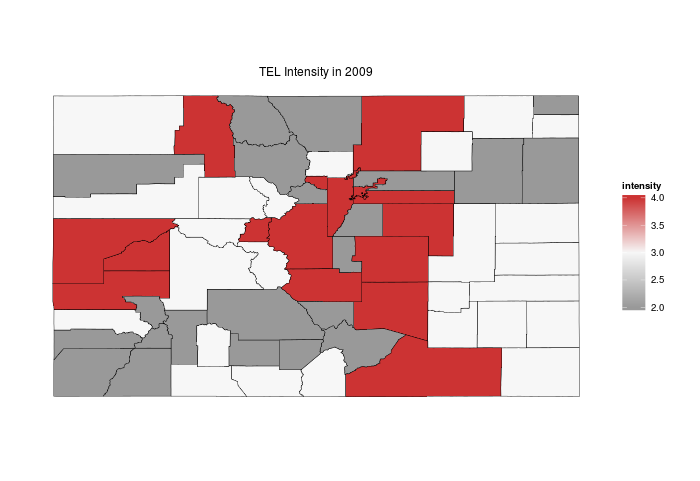
\includegraphics[width=1\textwidth]{/home/choct155/projects/TEL/ipynb/TEL_intensity_2009}
\par\end{centering}

Grey counties feature two overlapping TEL policies in 2009. White
counties feature three overlapping policies, and red feature four.
\end{figure}


While this score was a useful starting point, the subsequent measure
incorporates the county-specific dynamics captured in the third desired
characteristic: the likelihood of a binding constraint. The new score
was constructed based upon comparing the property tax base growth
to the limit imposed by the conjunction of SLPTR and TABOR limits
when both apply in a given year. If only one or the other applies
(due to deBrucing) in a given county-year, then the limit is just
that which is imposed by the policy in effect. The construction of
a composite limitation variable is useful because\emph{ only one of
the limits can be binding in any given county-year.} To get a sense
for why this occurs, Figure \ref{fig:Visual-Rationale-for-Comp-Limit}
plots the limits of both TABOR and SLPTR over time for Adams County.

\begin{figure}


\caption[Need for a Composite Limit]{Visual Rationale for a Composite Limit\label{fig:Visual-Rationale-for-Comp-Limit}}


\centering{}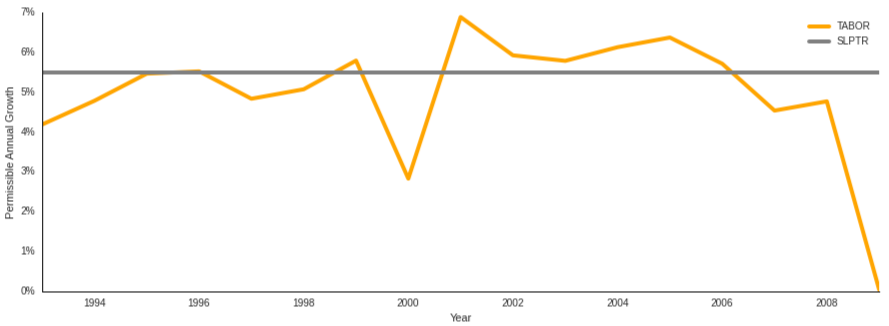
\includegraphics[width=1\textwidth]{/home/choct155/projects/TEL/ipynb/TABOR_vs_SLPTR}
\end{figure}


If the difference between the TABOR constraint and the SLPTR constraint
is negative (TABOR less SLPTR), it indicates that TABOR was the dominant
in a given county-year. This is the kind of interaction, referenced
earlier, that does not lend itself to easy capture by the existence
paradigm of representing TELs. The TABOR/SLPTR constraint has been
calculated as the minimum between the two for each county-year. Given
this composite limit, we can consider the impact on the property tax
revenue raising capacity of a given county in year $t$.

\begin{model}


\caption[Property Tax Constraint]{Property Tax Subject to TABOR/SLPTR\label{mod:Property-Tax-Subject-to-TABOR}}


\smallskip{}


\begin{centering}
$PropRev_t = MRate_t* AsmtRatio_t * BaseVal_t$
\par\end{centering}

\smallskip{}


\begin{centering}
s.t. $PropRev_t\leq (1 +\mathrm{min}(.055,CPI_t + NewConstr_t)) * PropRev_{t-1}$
\par\end{centering}

\smallskip{}


where
\begin{description}
\item [{$\hspace{1 cm}\bf{PropRev_t}$}] \begin{raggedright}
is the property revenue yield
in year $t$.
\par\end{raggedright}
\item [{$\hspace{1 cm}\bf{MRate_t}$}] \begin{raggedright}
is the millage rate in year $t$.
\par\end{raggedright}
\item [{$\hspace{1 cm}\bf{AsmtRatio_t}$}] \begin{raggedright}
is the proportion of the asset's
value that is considered taxable in year $t$, otherwise known as
the assessment ratio.
\par\end{raggedright}
\item [{$\hspace{1 cm}\bf{BaseVal_t}$}] \begin{raggedright}
is the market value of the asset
in year $t$.
\par\end{raggedright}
\item [{$\hspace{1 cm}\bf{CPI_t}$}] \begin{raggedright}
is the general change in prices (as
indicated by the Consumer Price Index change) between years $t-1$
and $t$.
\par\end{raggedright}
\item [{$\hspace{1 cm}\bf{NewConstr_t}$}] \begin{raggedright}
is the change in the housing
stock volume between years $t-1$ and $t$.
\par\end{raggedright}
\end{description}
\raggedright{}Note: The value of .055 refers to the 5.5\% Statewide
Limit on Property Tax Revenue (SLPTR).
\end{model}


The Model \ref{mod:Property-Tax-Subject-to-TABOR} governs the property
tax revenue yield for each and every county subject to TABOR and the
SLPTR in the absence of a local override. Given that the millage rate
is subject to explicit voter approval and the assessment ratio is
set at the state level, the economic activity within a county is the
relevant action to focus on when questioning whether or not the composite
limit will be breached. In other words, absent some sort of deBrucing
vote which would allow for increased revenue, the growth in the value
of the base should be compared to the composite limit to determine
whether or not the limit will be breached.\footnote{The residential assessment rate was 12.86\% in 1993. It fell four
times during the study period to 10.36\% (1995), 9.74\% (1997), 9.15\%
(2001), and 7.96\% (2003).} The value of the TABOR component of the constraint (second argument
in the minimization function) utilizes CPI-U data from the Bureau
of Labor Statistics and housing count information contained in the
demographic profiles constructed by the Colorado Department of Local
Affairs.\footnote{The query tool for the database containing demographic profiles by
county is located here: https://dola.colorado.gov/demog\_webapps/psParameters.jsf?counties=T.}

The market value of the base (both residential and non-residential)
may itself be decomposed further.

\begin{model}


\caption[Property Base Value]{Value of the Property Base\label{alg:Prop-Base-Val}}


\smallskip{}


\begin{centering}
$$BaseVal_t = Stock_t + AvgValue_t$$
\par\end{centering}

\smallskip{}


where
\begin{description}
\item [{$\hspace{1 cm}\bf{BaseStock_t}$}] is the count of property units
in year$t$. 
\item [{$\hspace{1 cm}\bf{AvgValue_t}$}] is the average value of property
in year$t$.\end{description}
\end{model}


Ideally, we would construct the value of the base of each county from
the components in Equation \ref{alg:Prop-Base-Val}, but we do not
have this data available (particularly on the non-residential side).
The approach taken leverages the relationship in Equation \ref{alg:Market-Value-Hack}
to back into market value, which is a useful figure for thinking about
economic activity in a county. It is important to note that because
assessments are generally susceptible to discretionary definition,
the assessment base can generally become uncoupled with market value.
In this instance, however, the potential for this decoupling is reduced.
In the absence of a deBrucing vote, local officials cannot raise revenue
by changing assessment rates or values. The real deficiency with this
approach is the downside risk. Assessment values can decline if the
yield is too high. Thus, it is certainly not a perfect proxy for value,
but it is a better fit than it would be in other situations. In interpreting
the analysis, one must also recognize that assessments take into account
exemptions, which decrease the assessment value by a fixed amount
relative to market value.

That being said, in 2014, the Colorado Legislative Council contracted
Wildrose Appraisal Incorporated to evaluate the assessment to sales
ratios by county. Among other things, the county-specific reports
include the median ratios for four property classes by county: Commercial/Industrial,
Condominium, Single Family, and Vacant. These ratios (where provided)
can be seen in Figure \ref{fig:Assessment-to-Sales}. The median ratio
manages to cluster about one fairly well. This suggests that the extent
of the divergence between assessment and market value is limited.

\begin{model}
\caption[Market Value Hack]{Market Value Hack\label{alg:Market-Value-Hack}}


\smallskip{}


\begin{centering}
$$MrktVal_t =\frac{AsmtVal_t}{AsmtRate_t}$$
\par\end{centering}

\smallskip{}


where
\begin{description}
\item [{$\hspace{1 cm}\bf{MarktVal_t}$}] is the total market value of
the base (residential or non-residential) in year$t$.
\item [{$\hspace{1 cm}\bf{AsmtVal_t}$}] is the assessment base value (residential
or non-residential) in year$t$.
\item [{$\hspace{1 cm}\bf{AsmtRate_t}$}] is the assessment rate (specific
to residential or non-residential) in year$t$.\end{description}
\end{model}


The property value dynamics vary dramatically over space and time
within Colorado. Data on assessment value by property type and the
assessment rates by residential and non-residential property has been
collected from the Colorado Division of Local Affairs, and it covers
every county during the 1993-2009 period.\footnote{Thank you to Denise Castro of the Division of Property Taxation.}
Ultimately, changes in the assessment base are the most relevant,
insofar as they are more directly limited by the composite constraint
than market value. By comparing assessment value growth with the allowable
growth under the composite limit, we can construct two ``COTEL intensity''
variables.
\begin{description}
\item [{$\bf{intensity\_flow}$}] is the\emph{ single-year} difference,
percentage change in assessment value less the percentage of allowable
revenue growth under the composite limit.
\item [{$\bf{intensity\_stock}$}] is the\emph{ cumulative} difference,
percentage change in assessment value less the percentage of allowable
revenue growth under the composite limit.
\end{description}
Both intensity variables seek to capture the fiscal stress caused
by TABOR and SLPTR. The higher the values of either, the more binding
the constraint and, therefore, the higher the level of fiscal stress.
$intensity\_stock$ is of particular interest, the hypothesis here
being that it captures a growing disparity between the economic activity
that occurs in a given county and the governmental capacity to facilitate
and/or regulate said activity. For example, one would expect it to
be more costly to govern a county of 50,000 people relative to a county
of 1,000 people. There are simply more interactions, both social and
economic, to mediate. The need for infrastructure grows, as does the
need to finance a larger educational demand. These constraints, then,
act as an instrument to decouple the trajectories of revenue potential
and expenditure need. The author expects this to be a dynamic effect. 

The relationship between the flow and intensity measures can be seen
in Figure \ref{fig:COTEL-Intensity-Adams}. It depicts measures of
intensity flow and stock for Adams County over the study period. Insofar
as the flow measure moderates the rate of change in the stock measure,
it may be though of as approaching the derivative. In this case, however,
it is at best a weak analogy because both measures have a lower bound
of zero. Adams County exempted themselves from both TABOR- and SLPTR-related
restrictions in 2002.

It is important to recognize that the intensity measurements will
generally be underestimated. The reason is that our market value concept
is derived directly from the assessment value and rate. As mentioned
previously, increases in assessment must be accompanied by a deBrucing
vote, so there is a natural obstacle to assessment rates rising faster
than market values. However, since there are no constraints on lowering
assessment value, there is a threat that assessment values (and thus
our concept of market value) will grow at a lower rate than actual
market value. In effect, any findings in this analysis related to
TEL intensity are likely to be conservative.


\subsection{The Gallagher Ratio}

Since the actions imposed by TABOR and SLPTR were conceptually similar,
they lent themselves to integration. GA, by constrast, was modeled
separately as simply the ratio between the residential and non-residential
tax bases within a county. The idea here was to capture the impact
of disparities between county ratios and the statewide ratio used
to calculate allowable assessment rates. If a given county has a higher
proportion of residential assessment value in its base, we would expect
it to have a more difficult time raising revenue, since the residential
assessment rates are held down to keep them consistent across the
state. Conversely, higher proportions of non-residential assessment
value serve to subsidize residential taxpayers in a given county,
since only so much yield is required and their assessment ratios cannot
be increased. The data required to construct this ratio come from
the assessment information discussed in Subsection \ref{sub:TABOR-and-SLPTR-Measure}.
The distribution of this Gallagher Ratio can be seen in Figure \ref{fig:Gallagher-Ratio-Dist}.
Clearly the variation seen here suggests that county circumstances
drive substantial variation in the impact of the Gallagher Amendment.

\begin{figure}
\caption[Gallagher Ratio]{Variation in the Gallagher Ratio\label{fig:Gallagher-Ratio-Dist}}


\centering{}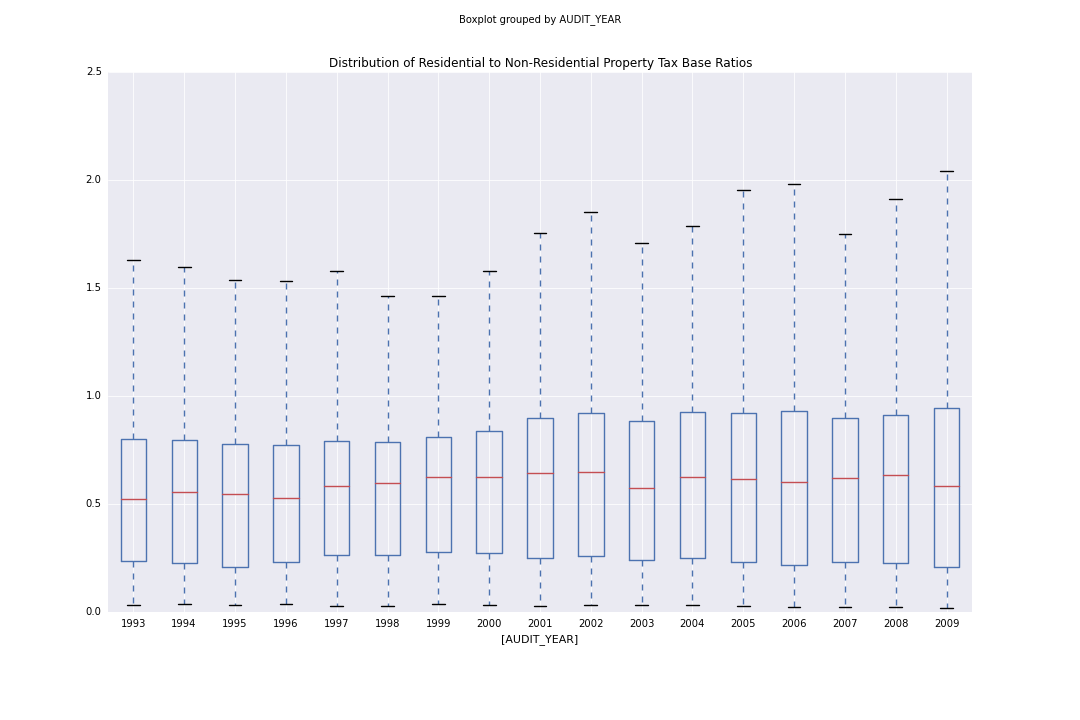
\includegraphics[width=1\textwidth]{/home/choct155/projects/TEL/ipynb/prop_ratio_dist}
\end{figure}



\section{The Implications of Space}
\begin{quotation}
``{[}T{]}he first law of geography: everything is related to everything
else but near things are more related than distant things.''\citep{Tobler1979}
\end{quotation}
That a given data generating process may yield observations that are
related to each other is not a new concept by any stretch of the imagination.
So central has this concern been in the modern practice of statistical
analysis, large swaths of theoretical development are devoted to methods
of mitigating this confounding factor. The foundational model in econometrics
- ordinary least squares - assumes it away with the assertion of independent
observations for conceptual tractability. The analysis of real world
data, however, often necessitates meeting this issue head on with
a host of models designed to deal with this basic deviation from ``well
behaved'' data.

The concern centers on the fact that, though approaches differ substantially,
statistical estimation can generally be distilled down to a search
for conditional expectation. The observed data have some central tendency,
and each of the statistically significant variables that act on the
system cause some sort of deviation from that central tendency. Measuring
the deviation from that baseline expectation requires that the baseline
be consistent throughout the observational space. If one desires to
understand the relative heights of five people, he/she should either
ensure they all stand on level ground, or capture five observation-specific
adjustments that yield the same effect.

An important lesson that the field has learned is that variance in
this baseline is not a deal breaker. If the relationship is systemic
and estimable, the effect can be accommodated. The desire to understand
when this stable reference can be relied upon is a strong argument
for the establishment of stationarity. If we know that the relationship
between observations follows a consistent joint distribution, or some
reasonable facsimile, we can reliably estimate the impact of variables
that impact the system.


\subsection{Space as a Factor in Inference}

Autocorrelation and autoregression are sometimes differentiated in
the literature, but often conflated. In many cases the former refers
to serial correlation in the errors, while the latter refers to correlation
in observations.\citep{Tsay2005} We will use this distinction in
this study, but in reality, scholars often use autocorrelation to
describe correlation in both the errors and the observed values. Our
definitional split will facilitate discussion of the implications
of these two behaviors.

Given the split we have defined, the two are not necessarily linked,
insofar as an autoregressive process is only one potential cause of
correlation in the error term. Other factors, like additional variables
that have impacts lasting longer than one period, can also contribute
to autocorrelation. This is a theoretically important distinction,
insofar as unbiased estimates are still possible with uncorrelated
observations, albeit inefficiently. In practice, however, they tend
to occur jointly.
\begin{quotation}
``In fact, as Wold showed, when all the sample serial correlations
of the {[}independent variables{]} are zero the estimates of variance
given by the least squares method are strictly unbiased whether the
errors are serially correlated or not. It seems to us doubtful, however,
whether this result finds much application in practice. It will only
rarely be the case that the independent variables are serially uncorrelated
while the errors are serially correlated.''\citep{Durbin_Watson1950}
\end{quotation}
The concept of autocorrelation was first explored in time series analysis.
Cochrane and Orcutt are among the early commenters on the dangers
of failing to account for this behavior. Mitigation of this behavior
proceeded in a task-specific fashion, designed to restore the assumption
base of OLS.
\begin{quotation}
``If we have a relationship in which the error term is autocorrelated,
it has been shown by Aitken {[}...{]} that the method of least squares
still yields the best linear unbiased estimates of the regression
coefficients provided the lack of independence in the error series
is taken into account. One method of overcoming this lack of independence
is to make the error term random by transforming all the variables
according to the autoregressive structure of the error term.''\citep{Cochrane_Orcutt1949}
\end{quotation}
If autocorrelation is not explicitly addressed, variance in the estimates
is generally larger and the standard procedure for understanding the
variability in the estimates is no longer applicable.\citep{Durbin_Watson1950}
Failing to account for an autoregressive process causes substantially
more damage. Consider a noiseless autoregressive process.

\begin{model}


\caption[Noiseless AR(1)]{Noiseless Autoregressive Process\label{alg:Noiseless-AR1}}


\vspace{10bp}


\begin{centering}
$y_t =\Gamma y_{t-1} +\beta X_t$
\par\end{centering}

\vspace{10bp}


SEE IF THE AUTOREGRESSIVE EFFECT CHANGES ACROSS TABOR PASSAGE WITH
A COUPLE KEY VARIABLES OF INTEREST. DISCONTINUITY REGRESSION...

ALLOWS US TO ISOLATE THE WEDGE BETWEEN REGIMES, THAT'S WHAT SHOULD
BE TAKEN OUT INSTEAD OF THE ENTIRE AUTOREGRESSIVE TERM...

IF THERE IS NO DIFFERENCE, IGNORE IT. IF THERE IS, THAT'S GRAVY...
\end{model}


If the first term on the right hand side is omitted, the model is
misspecified. In effect, the problem is one of omitted variable bias.
By failing to account for all of the structurally relevant regressors,
we have limited our ability to generate an unbiased estimate of the
phenomenon of interest. If consumption of good A is a function of
the prices of both good A and good B, we cannot reliably estimate
consumption of A based solely on the price of A or B in isolation.

Spatial dependence shares a great deal of the conceptual domain occupied
by temporal dependence. Similar problems of inefficiency and bias
arise in the context of spatial autocorrelation and the failure to
correctly specify a spatially autoregressive process. Anselin (1999)
presents three primary reasons why spatial dependence must be incorporated
when present\citep{Anselin1999}:
\begin{enumerate}
\item ``The 'structure' behind the instability is\emph{ spatial} (or geographic)
in the sense that the location of the observation is crucial in determining
the form of the instability.'' In such cases, we can expect heteroskedasticity
to be a function of spatial location, or coefficients to indicate
different slopes at different locations. Many phenomenon fit this
mold. If one were to model the impacts on real estate prices of a
given phenomenon, one better control for the location specific aspects
of the sample. Different price regimes and economic dynamics prevail
in different states, for example.
\item ``{[}B{]}ecause the structure is spatial, heterogeneity often occurs
jointly with spatial autocorrelation, and standard econometric techniques
are no longer appropriate.'' This condition mirrors directly the
variance-related issues for temporal autocorrelation mentioned above.
\item ``In a single cross-section, spatial autocorrelation and spatial
heterogeneity may be observationally equivalent.'' Spatial heterogeneity
as used by Anselin refers to a spatially autoregressive process. Since
these two phenomena can look the same, it is not clear at the outset
if we are worried only about loss of efficient estimation of parameters
(which is a non-trivial concern) or bias due to misspecification.
Anselin suggests that analysts model both in all cases.
\end{enumerate}
One major difference between temporal and spatial dependency is dimensionality.
Whereas lags move along one dimension in the temporal context, lags
move in all three cartesian dimensions in the spatial context. Figure
\ref{fig:Space-Time-Memory}, which identifies each lag with a consistent
shade of blue, illustrates the concept. Conseqeuntly, ``in contrast
to the unambiguous notion of a 'shift' along the time axis, there
is no corresponding concept in the spatial domain.''\citep{Anselin1999}
The approach taken has been to use a spatial lag operator that captures
a weighted average of values from all spatial features in the local
neighborhood $W$.

\begin{figure}


\caption[Memory in Space \& Time]{Parallelism in Temporal and Spatial Dependency\label{fig:Space-Time-Memory}}


\centering{}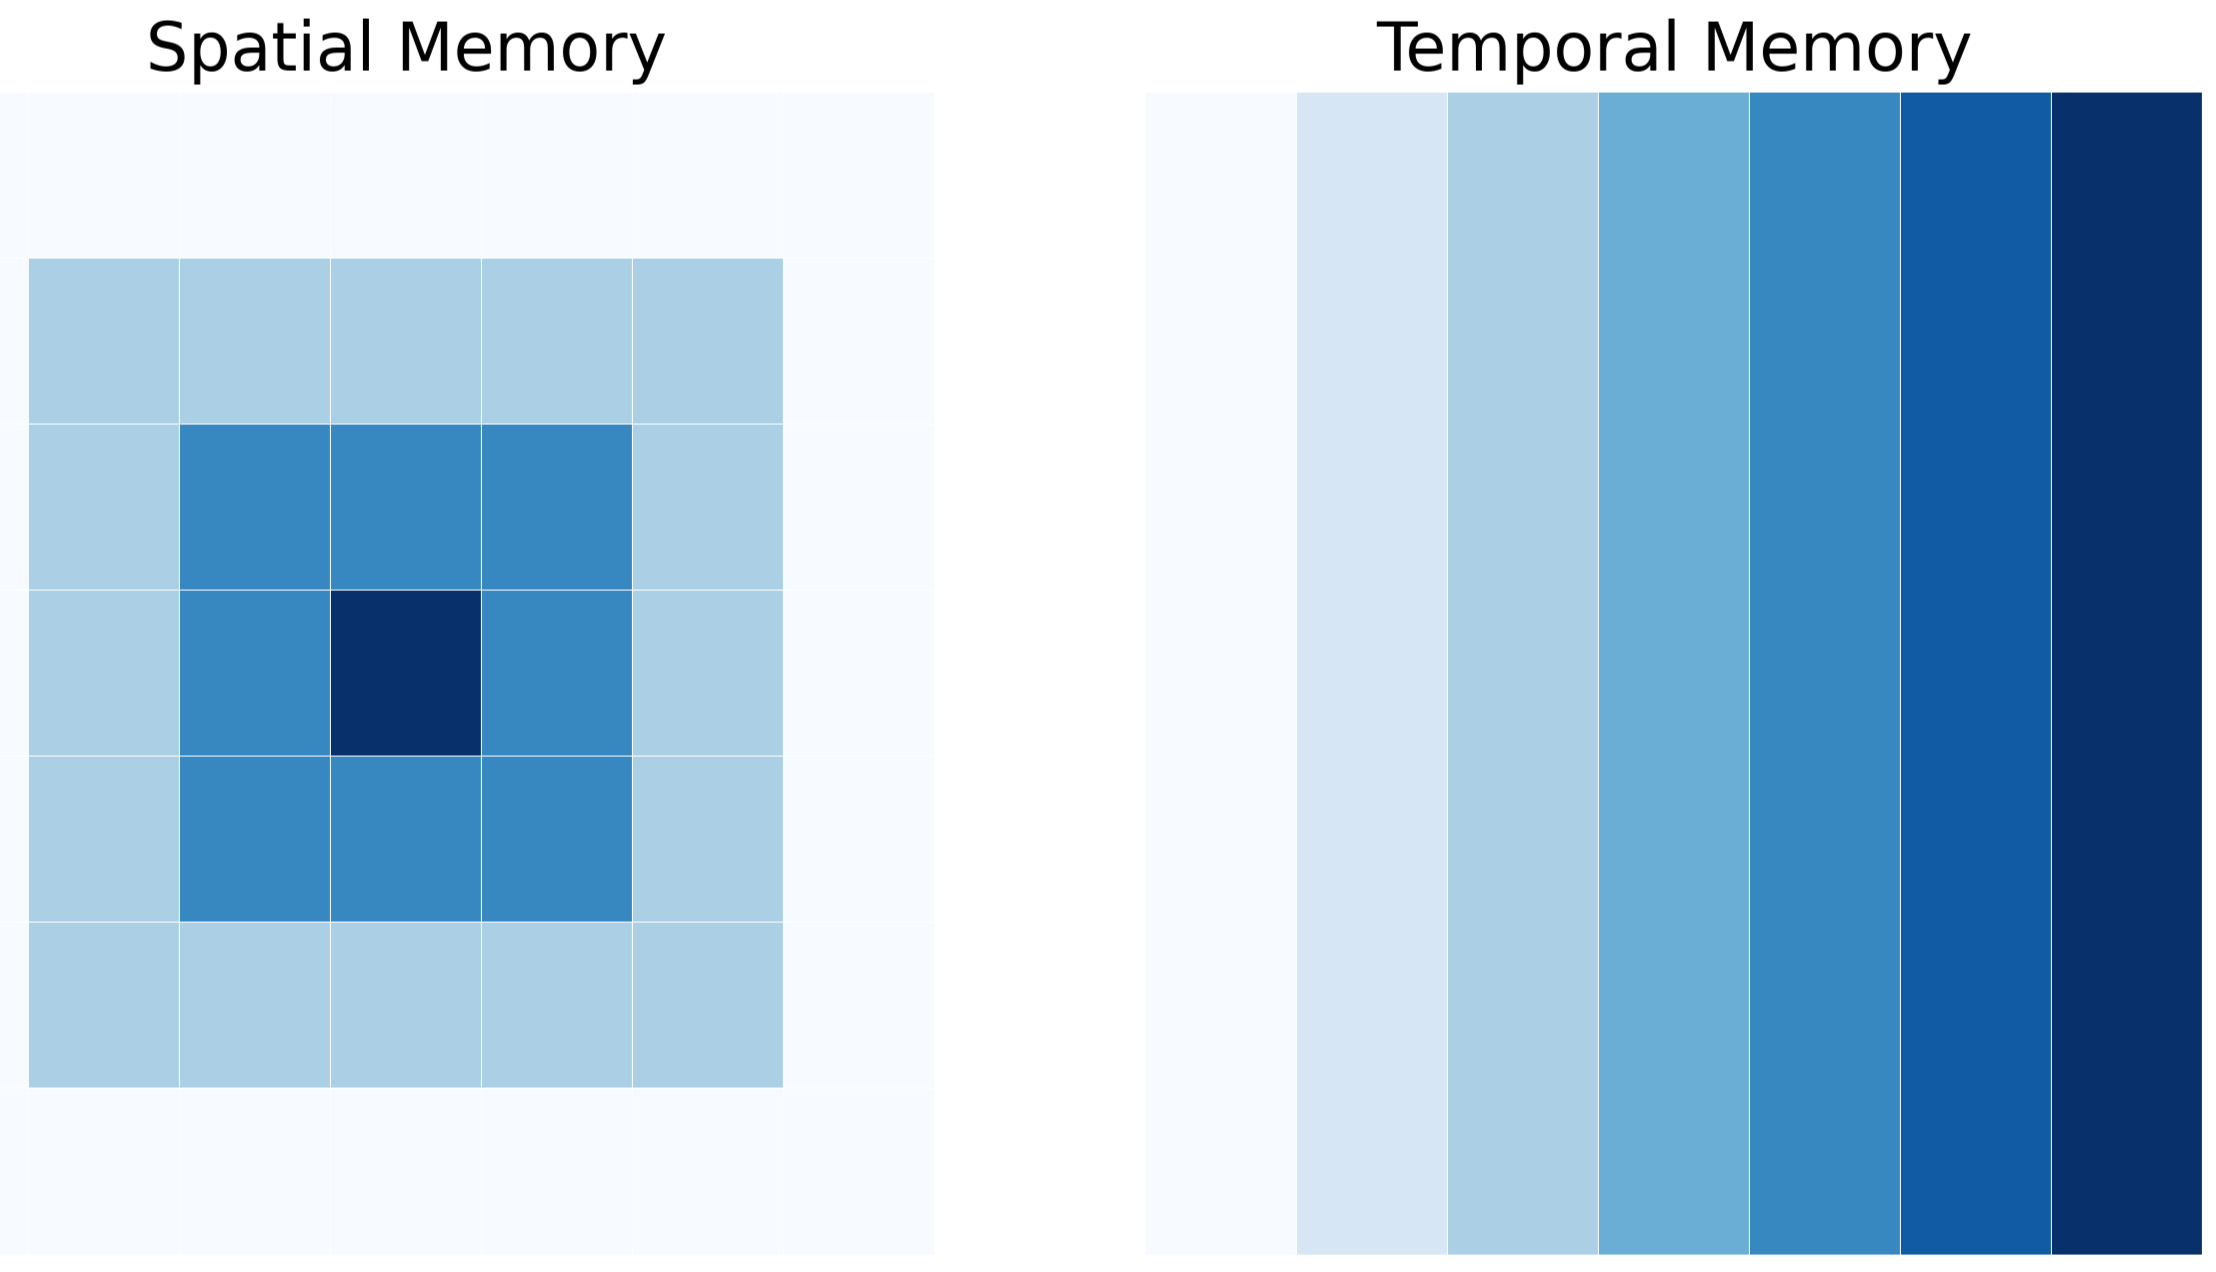
\includegraphics[width=1\textwidth]{figures/space_time_memory}
\end{figure}


One might reasonably ask, why bother with the trouble of estimating
spatial lags? Could we not use a more conventional method like fixed
or random effects at the county level to control for the impact of
neighboring counties? There are two reasons why this analysis has
not gone this route. First, whether it be through repeated cross-sectional
or panel analysis, this study is concerned with variation in circumstance
over time. In a fixed effect or random effect world, one is faced
with a decision about the scope of the effect to remove from each
observation. If we keep the scope within county and do not vary the
effect across time, we implicitly assume that the impact of neighbors
does not change over time. If we allow for a two-way effect, we run
the risk of washing out the uniqueness of the county. Remaining variable
impacts would be of note, but the effect would likely be muted. Modeling
neighborhood impacts directly avoids wrestling with these unpleasantries,
at least in the context of neighborhood effects. To be sure, fixed
effects are employed in some situations that follow, but direct modeling
of neighborhood effects gives us more flexibility.

Second, fixed and random effects are both model parameters to be estimated.
Consequently, in these situations, we must be concerned with degrees
of freedom. Generally, the safe bet is to have many observations per
group, so that said parameters may be reliably estimated. In the two-way
scenario above, we wittle that observation count down to one for each
county-year effect.

Third, fixed and random effects are useful ``catch-alls'' when the
model is incorrectly specified. They are meant to be proxies for those
elements that are not included in the specification. Due to their
scope of application, one cannot parse out the impact of individual
components of said effects. In general, it is preferable to model
the specific phenomenon directly when possible (in this case, neighborhood
effects).

Finally, as Anselin and Arribas-Bel note, the spatial fixed effect
approach only mitigates spatial dependence in certain situations.\citep{Anselin2011}
In particular, ``unless there are strong theoretical or practical
reasons why distance decay should be ruled out, the use of spatial
fixed effects will not be sufficient to correct for the presence of
spatial correlation.'' Admittedly, there is only limited use of weight
matrices that exhibit kernel decay in this study, but we do expect
that distance will erode the effect on a given county. Consequently,
the choice to model spatial dependency will better align with future
extensions of this work.


\subsection{Space as a Factor in Public Financial Theory}

Spatial considerations also have a direct impact on our conception
of public finance from a theoretical perspective. The more local the
scope of consideration, the more important these effects become. Bennet
(1980) identifies three main components that must be considered\citep{Bennett1980}:
\begin{description}
\item [{Tapering}] captures the notion that services are generally delivered
from a particular location. The farther one gets from this location,
the smaller the benefit one may experience from a service emanating
from said location. An easy example of this phenomenon is the provision
of local fire fighting services. The farther one resides from the
fire station, the longer it takes to consume the service in the event
of a fire. This lag is likely to lead to larger amounts of damage
if a fire is occurring. Thus, the expected benefit for residents who
live ``far'' from the station is lower than those that live ``near''
the station. This effect has implications for the definition of a
pure public good. Tapering inhibits the ability to provide a service
uniformly. Even if resources were such that all fire calls at any
given time could be accommodated, a form of rivalry has creeped into
the picture. Stochastic consumption of fire services is more heavily
consumed as a function of spatial proximity.
\item [{Jurisdictional~Partitioning}] creates differentials in service
delivery across localities. This is not inherently a bad thing. Indeed,
Tiebout leverages this phenomenon to argue that differentiation is
efficient.\citep{Tiebout1956} We must, however, acknowledge that
resource disparities do exist and jurisdictional boundaries neatly
capture the joint distribution of resources, service costs, and service
delivery. The more important element is an extension of this differentiation.
An optimal jurisdictional area would efficiently capture the tax-expenditure
bundle preferred by the constituents, and the optimal size for a jurisdiction
is that which accords with the optimal range for delivery of the services
rendered. To continue the fire services example, at some distance
$x$ from the station, the cost of transporting fire fighting resources
outweighs the damage from a fire (to choose a particularly callous
metric). Efficient jurisdictional size would be driven by the boundary
at which the marginal benefit of service delivery and the marginal
cost of fire damage are equivalent.\footnote{Obviously this concept is complicated dramatically by political considerations
and the existence of many services to deliver. The point, however,
is made.} In general, service range, a spatial concept, is important.
\item [{Spillover}] stems from jurisdictional partitioning. ``{[}I{]}t
is not possible to completely separate the 'service club' of one jurisdiction
from another, not only because of tapering effects, but also because
of the general mobility of people in modern economies who often live
in one jurisdiction, work in another, and seek leisure and shopping
outlets in yet others.''\citep{Bennett1980} In general, the activities
of one jurisdiction have significant implications for the choices
of residents sited in a nearby jurisdiction. Indeed, this is the major
motivation for the inclusion of spatial dependency in this study.
\end{description}
At a basic theoretical level, lack of uniformity driven by spatial
considerations violates the absoluteness of non-excludability and
non-rivalry. From an applied perspective, it is materially difficult
to separate the industrial bases, preferences, and activities of neighboring
jurisdictions when seeking to explain fiscal behavior. In truth, there
are many examples of coordination across jurisdictions that are facilitated
by spatial proximity. For all of these reasons, the case against at
least exploring spatial effects in the analysis of fiscal behavior
becomes increasingly untenable.

\clearpage


\chapter{Implications for Revenue Yield and Capacity\label{chap:RevYieldCapacity}}


\section{Introduction}

The economic potential of any system is not only driven by the presence
of natual and/or developed capital, but also the institutions that
govern the exploitation of these valueable assets. In this sense,
the term economic potential is misleadingly incomplete. The mechanism
that drives resource allocation is a function of both the distribution
of purely economic value and the feasible range of activities governed
by political institutions. The goal of institutional design for economic
growth, therefore, ought to be the facilitation of those activities
that increase the marginal product of ``value extraction'' efforts.
If the objective is the maximization of economic growth, this broad
goal is unlikely to draw many detractors. The devil, however, is in
the details. The major challenge for any fiscal manager is operating
under institutional constructs that reflect in one way or another
the will of the constituents, while also achieving the expected fiscal
outcomes. This task is challenging because these concepts are not
separable.
\begin{quotation}
``Once the fiscal policy objectives or targets are decided upon government
tries to implement them by using policy parameters, such as tax rates,
subsidies, transfers, purchases and other types of government expenditures
over which it has conrol. These parameters are known as instruments.
Policy targets and instruments belong to the same economic system.
The former are endogenous and the latter are pre-determined. The values
policy targets take depend on the type of instruments employed, and
the relation between them will be determined by the structure of the
economy.''\citep{Atul_Tulasidhar1984}
\end{quotation}
Among the multitude of policy innovations that have been advanced
in service of increasing economic growth, institutional reforms that
act on the property tax base have materially altered local government
finance for more than a century. As early as the 1880s, these reforms
were dominated by efforts to target specific populations.\citep{Bowman2008}
However, starting in large part with the Tax Revolt of the 1970s,
more interest has taken root in implementing reforms that target the
base in a general way: the tax and expenditure limitations discussed
in the preceding sections. The impact of these and other measures
has been noticeable. While property tax revenue remains fairly buoyant
with respect to the economy, it has declined in importance from a
proportional contribution perspective.

This paper is the first empirical section of the study. It seeks to
evaluate the relationship between COTELs and homogeneity in revenue
behavior across counties. In 1956, Tiebout suggested that choice among
local jurisdictions was an efficiency enhancing characteristic of
a federal system. Choices only exist to the extent that variety exists
among the available alternatives. This paper intends to shed some
light on whether or not COTELs affect the variety among the jurisdictional
choices of local residents. A decrease in said variety will be referred
to as ``fiscal convergence''. We will pursue this task by employing
the operationalization of COTEL intensity discussed in Subsection
\ref{sub:TABOR-and-SLPTR-Measure}. This concept is designed to capture
the magnitude of the composite restriction of both TABOR and SLPTR.
The impact of GA, by contrast, will enter the analysis as a standalone
variable.


\section{What is the Significance of Revenue Yield and Capacity?\protect\footnote{As used here, revenue yield signifies the actual, realized revenue
collected by a given jurisdiction. Revenue capacity, by contrast,
captures the economic potential of the tax base. We may think of this
concept as the abstract revenue yield for a given county at some standard
level of tax effort. If, for example, the property in county A is
more expensive than the property in county B, county A can collect
more revenue than county B with the same level of tax effort. In this
example, county A has greater revenue capacity than county B.}\label{sec:Rev-Significance}}

This study focuses on local revenue behavior, so perhaps it behooves
us to ask whether or not local own-source revenues are really all
that important. Why can local governments not rely on intergovernmental
fiscal transfers from higher levels of government to satisfy their
finance needs? Wallace Oates considers arguments for and against the
importance of local revenue yield and capacity in some detail.\citep{Oates2001}

For starters, from a Tiebout perspective, local revenue instruments
are important because they act as prices for local constituents. They
are the costs incurred by taxpayers in exchange for the consumption
of local public services. Costs lead consumers to perform triage.
Without costs, the strong monotonicity assumption is permitted to
run wild. In other words, constituents would seek to consume without
limit. It is the provision of local revenue by taxpayers that reveals
opportunity cost and forces them to reveal their preferences. In so
doing, they provide the information required by local fiscal managers
to make smart choices in service of satisfying voter preferences.

\begin{tabular}


\caption[Monotonicity]{Weak and Strong Monotonicity\label{alg:Weak-and-Strong-Monotonicity}}


\vspace{10bp}


\begin{centering}
\emph{\noun{Weak Monotonicity:}}\emph{ If} $x\geq y$\emph{ then}
$x\succeq y$.
\par\end{centering}

\begin{centering}
\emph{\noun{Strong Monotonicity:}}\emph{If} $x\geq y$\emph{ and}
$x\neq y$,\emph{ then} $x\succ y$.
\par\end{centering}
\begin{quotation}
``Weak monotonicity says that 'at least as much of everything is
at least as good'. If the consumer can costlessly dispose of unwanted
goods, this assumption is trivial. Strong monotonicity says that at
least as much of every good, and strictly more of some good, is better.
This is simply assuming that goods are good.''\citep{Varian1992}\end{quotation}
\end{tabular}


As discussed in Subsection \ref{sub:SubFinance-Normative-Objectives},
local discretion over revenue sources is critical for local autonomy,
an ideal that has been advocated on practical and theoretical grounds.
Practical arguments extend back at least as far the debate over the
crafting of the US Constitution. The so-called Anti-Federalists argued
vociferously against the consolidation of power in central government.
They believed that not only was this a sure path to a tyrannical regime,
but also that it was remarkably impractical to try and govern so vast
and diverse a country from a single location. Representatives sent
to higher levels of government could not possibly reflect the rich
diversity of interests and needs that would inevitably fall within
their purview. From a theoretical perspective, local autonomy facilitates
the pursuit of the marginal equivalence of costs and benefits, an
efficiency enhancing feature that naturally seeks welfare maximization
for society.

Detractors could feasibly argue that marginal equivalence is not actually
possible because the costs of production are often uncoupled with
the means of financing public goods. Furthermore, given disparities
in resource endowments, there are limits to the volume and quality
of services that can be provided for some local jurisdictions, no
matter what their preferences are. For the sake of balance, we should
also note that the Federalists were greatly concerned by the potential
for material harm to minority ``factions'' if local autonomy was
too strong. Their bias towards central provision was cultivated in
part because they believed the multitude of opinions expressed at
higher levels of government would lead to fairer outcomes, in this
case fairer allocations of public resources. In the end, all that
seems to be clear is that either extreme appears to be undesirable.
Therefore, the role for local own-source revenue is an important one
that is worthy of study.


\section{What is the Expected Impact of TELs on Fiscal Convergence?}

Fiscal convergence in our context carries a spatial dimension. When
one considers the siting choice of a taxpayer, theoretically, the
entire set of local jurisdictions in the country is available to him
or her. In reality, however, the costs associated with all of these
choices is far from equal even when staying inside Colorado. Leaving
aside cost of living for the purposes of our analysis, the costs of
mobilization are non-trivial. It is much more costly for a resident
of the northeastern County of Logan to move to the southwestern County
of Montezuma, than it would be to move to the neighboring County of
Morgan. Thus, convergence in fiscal outcomes does not have to be uniform
across the entire state to have a significant impact. The activity
that occurs in the local neighborhood, the collection of counties
that are ``close'' to the county of interest, is the driving factor.
For this reason, we are concerned with the\emph{ clustering of fiscal
behavior within the local neighborhood.}

From a theoretical standpoint, there are two main features of COTELs
that would promote fiscal clustering among low-capacity jurisdictions
in particular. First, COTELs impose asymmetric pressure on revenue
yields over time. The rate of increase is limited by an explicit growth
limit, but decreasing yields are not so constrained. Furthermore,
once a drop in revenue has been experienced in one year, the baseline
is ``ratcheted'' down. The allowable revenue in the current year
is measured against only the previous year's revenue, and not the
long term trend. Low revenue years have a disproportionate impact
on the long-term revenue capacity of the jurisdiction.

The second impact is related to the first. To the extent that COTELs
bias revenue downward (in a manner quite uncoupled with demand projections),
it becomes increasingly difficult for constrained jurisdictions to
invest in the human and physical capital needed to support robust
economic growth. The first effect impacts revenue generation, while
the second impacts the capacity of the economic base itself.

A complicating factor is the existence of spillovers. Both the provision
of public goods and the economic vitality of neighboring jurisdictions
impact the fiscal and economic capacity of the primary jurisdiction.
This externality network has the potential to dynamically reinforce
economic growth behavior, whether it be a high or low growth regime.
If COTELs exacerbate this effect, there could be undesirable long-term
consequences for low capacity counties seeking to create the conditions
for economic growth. Insofar as the relationship between COTEL intensity
and spatial dependency is evaluated, this chapter explores this phenomenon
directly.


\section{How is Fiscal Clustering Measured?}

Testing whether or not the constraints imposed by COTELs lead to fiscal
convergence is difficult to achieve with the prevailing models in
this area. Most of the empirical work attempts to study TELs across
states, and as such, focuses on statewide definitions of TELs. This
tends to cover up local variation, but perhaps more interestingly,
this choice in geographic scope encourages certain kinds of questions.
What is the impact of TELs on revenue volatility?\citep{StClair2012}
Do TELs constrain property taxes?\citep{Dye_McGuire1997} Do TELs
constrain growth in public employment and wages?\citep{Poterba_Rueben1995}

Comparatively little research examines the within state dynamic. Once
one asks the question about local differences, modeling the parameter
of interest is a different game altogether. In this case, the researcher
must tease out variation among fiscal circumstances for which statewide
policy is a common denominator. Once this issue comes to the fore,
one is immediately confronted with the following question: if the
statewide policy does not vary cross-sectionally, do we expect uniform
impact across all jurisdictions at time $t$? Fiscal behavior is a
function of economic circumstance, and given the variation in economic
bases across a given state, one would expect COTELs to have different
impacts in different jurisdictions.

A second, and related, question is whether or not we expect a temporal
element in the impact of COTELs. Does the constraint placed on a county
increase with the amount of time the county has spent operating under
the COTEL? Furthermore, given the fact that the COTEL environment
is composed of overlapping policies, do we expect interaction effects
to play a role? To shed light on such questions, this study employs
spatial techniques to examine a panel dataset of county-level fiscal
and economic data in Colorado over the 1987-2009 time period (econometric
exploration begins in 1995). First, we establish the existence of
temporal variation in fiscal clustering, and then we employ econometric
techniques to uncover the impact of COTEL intensity and the Gallagher
Ratio.


\subsection{Does Fiscal Clustering Occur and Does it Change Over Time?}

The hypothesis rests on the idea that not only does spatial clustering
of fiscal behavior occur, the nature of the clustering must vary over
time. Without both of these conditions, there is no basis for measuring
the impact of COTELs on fiscal convergence. To determine whether or
not these conditions are met, we will take snapshots of fiscal and
economic hotspots\footnote{``Hotspots'' are pockets of similar values.}
every five years, starting with 1987. Fiscal hotspots are evaluated
via measurement of revenue yield per capita. Economic hotspots are
evaluated via annual payroll per capita.\footnote{From a spatial perspective, payroll is a superior measure of activity
relative to income. Income is a person-based measure, and thus may
be derived from neighboring jurisdictions if an individual commutes
some distance to their place of employment. Payroll, by contrast,
is a firm-based measure. Consequently, it is not capable of mobility
in the same sense.} The hotspots are identified with Local Indicators of Spatial Autocorrelation
(LISAs) developed initially by Getis \& Ord\citep{Getis_Ord1992},
with subsequent development by Anselin.\citep{Anselin1995} The measures
are Getis \& Ord's G{*} (GOG) and Local Moran's I (LMI), respectively.

To evaluate clustering, LISAs require a definition of the linkages
of importance between jurisdictions. Said differently, they require
an explicitly defined local neighborhood. Spatial analysis is generally
sensitive to the choice of weight matrices (which define the local
neighborhood), so we test multiple neighborhood criteria. Corroboration
across tests lends support to the findings.


\subsubsection{Weight Matrices\label{sub:Weight-Matrices}}

Weight matrices, in an abstract sense, define ``closeness''. The
definition of proximity can vary quite dramatically by application.
The most natural interpretation, the one employed in this study, is
based upon spatial proximity. However, it is quite plausible to use
other distance measures. For example, one might define neighbors as
those counties with similar demographics, industrial bases, or any
other characteristic of interest. Since the focus of this study is
on siting choice given the cost of mobility, spatial proximity is
a natural choice.

Taking spatial proximity as the weight basis, there are a number of
ways to define the neighborhood. This study employs two common approaches:
contiguity and distance. As one might expect, contiguity requires
contact to be considered a neighbor. Contact with the primary jurisdiction
is not strictly required. A second order contiguous neighborhood,
for example, would include neighbors that contacted a jurisdiction
in contact with the primary jurisdiction. Distance, by contrast, includes
as neighbors all jurisdictions within some distance of the primary
jurisdiction.

\begin{figure}


\caption[Weight Matrices]{Differing Weight Matrix Definitions\label{fig:Def-Weight-Matrix}}


\centering{}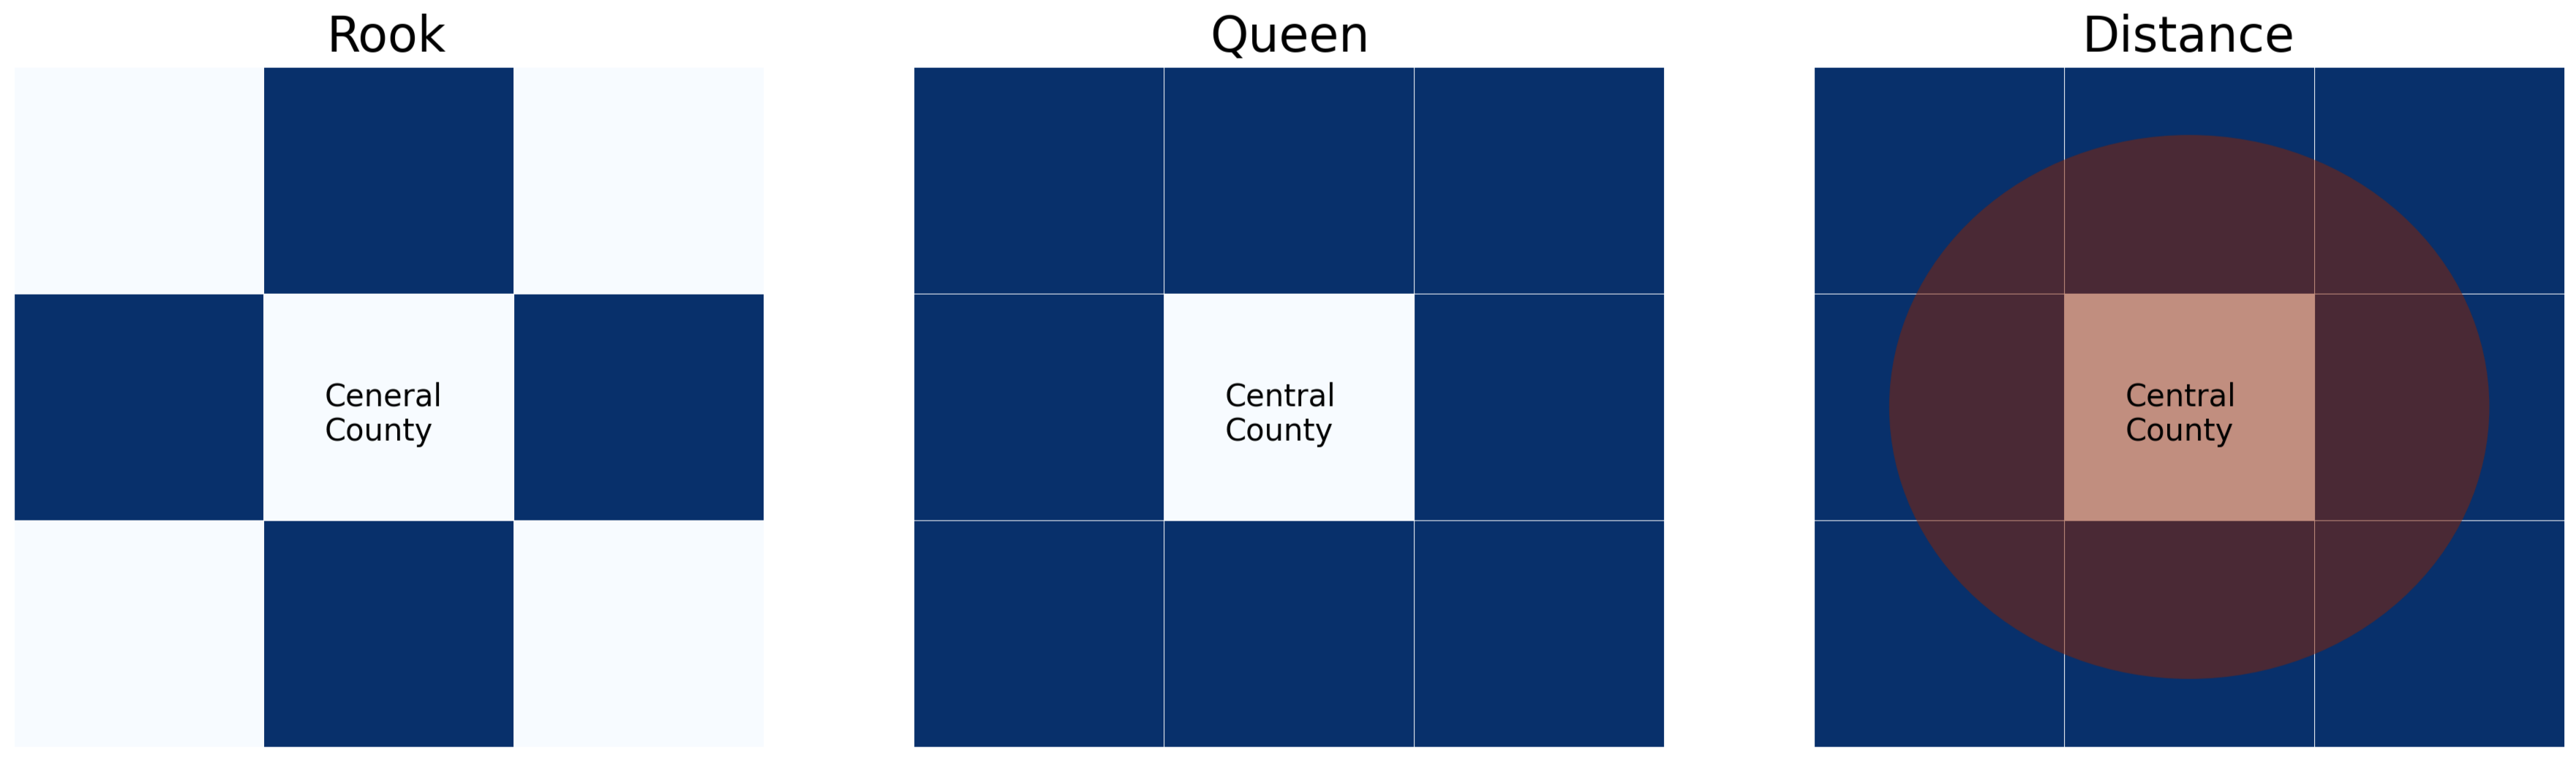
\includegraphics[width=1\textwidth]{figures/w_def}
\end{figure}


Within the contiguity and distance classes of weight matrices, there
are several variations on the theme. Figure \ref{fig:Def-Weight-Matrix}
shows two types of contiguous neighborhood definitions in the first
two panels: rook and queen. As can be seen, these definitions are
taken directly from the rules of chess. The third panel provides a
generic view of a neighborhood defined via a distance metric. In this
instance, distance is measured from the primary jurisdictions centroid,
but one could envision distance from the closest border or the population's
center of gravity being relevant metrics as well.

As depicted in Figure \ref{fig:Def-Weight-Matrix}, all of the weights
for each neighborhood are binary. Blue squares indicate weight values
of 1, so those jurisdictions are ``all in'', so to speak. Binary
classification of neighbors is in no way a requirement. The strength
of the weight may vary with proximity, and there are a number of decay
functions in common use. This study employs three kinds: binary, inverse
distance, and Gaussian. Generic examples of these are depicted in
Figure \ref{fig:Variance-in-Weights}.

\begin{figure}


\caption[Decay Curves]{Variance in Weight as a Function of Distance\label{fig:Variance-in-Weights}}


\centering{}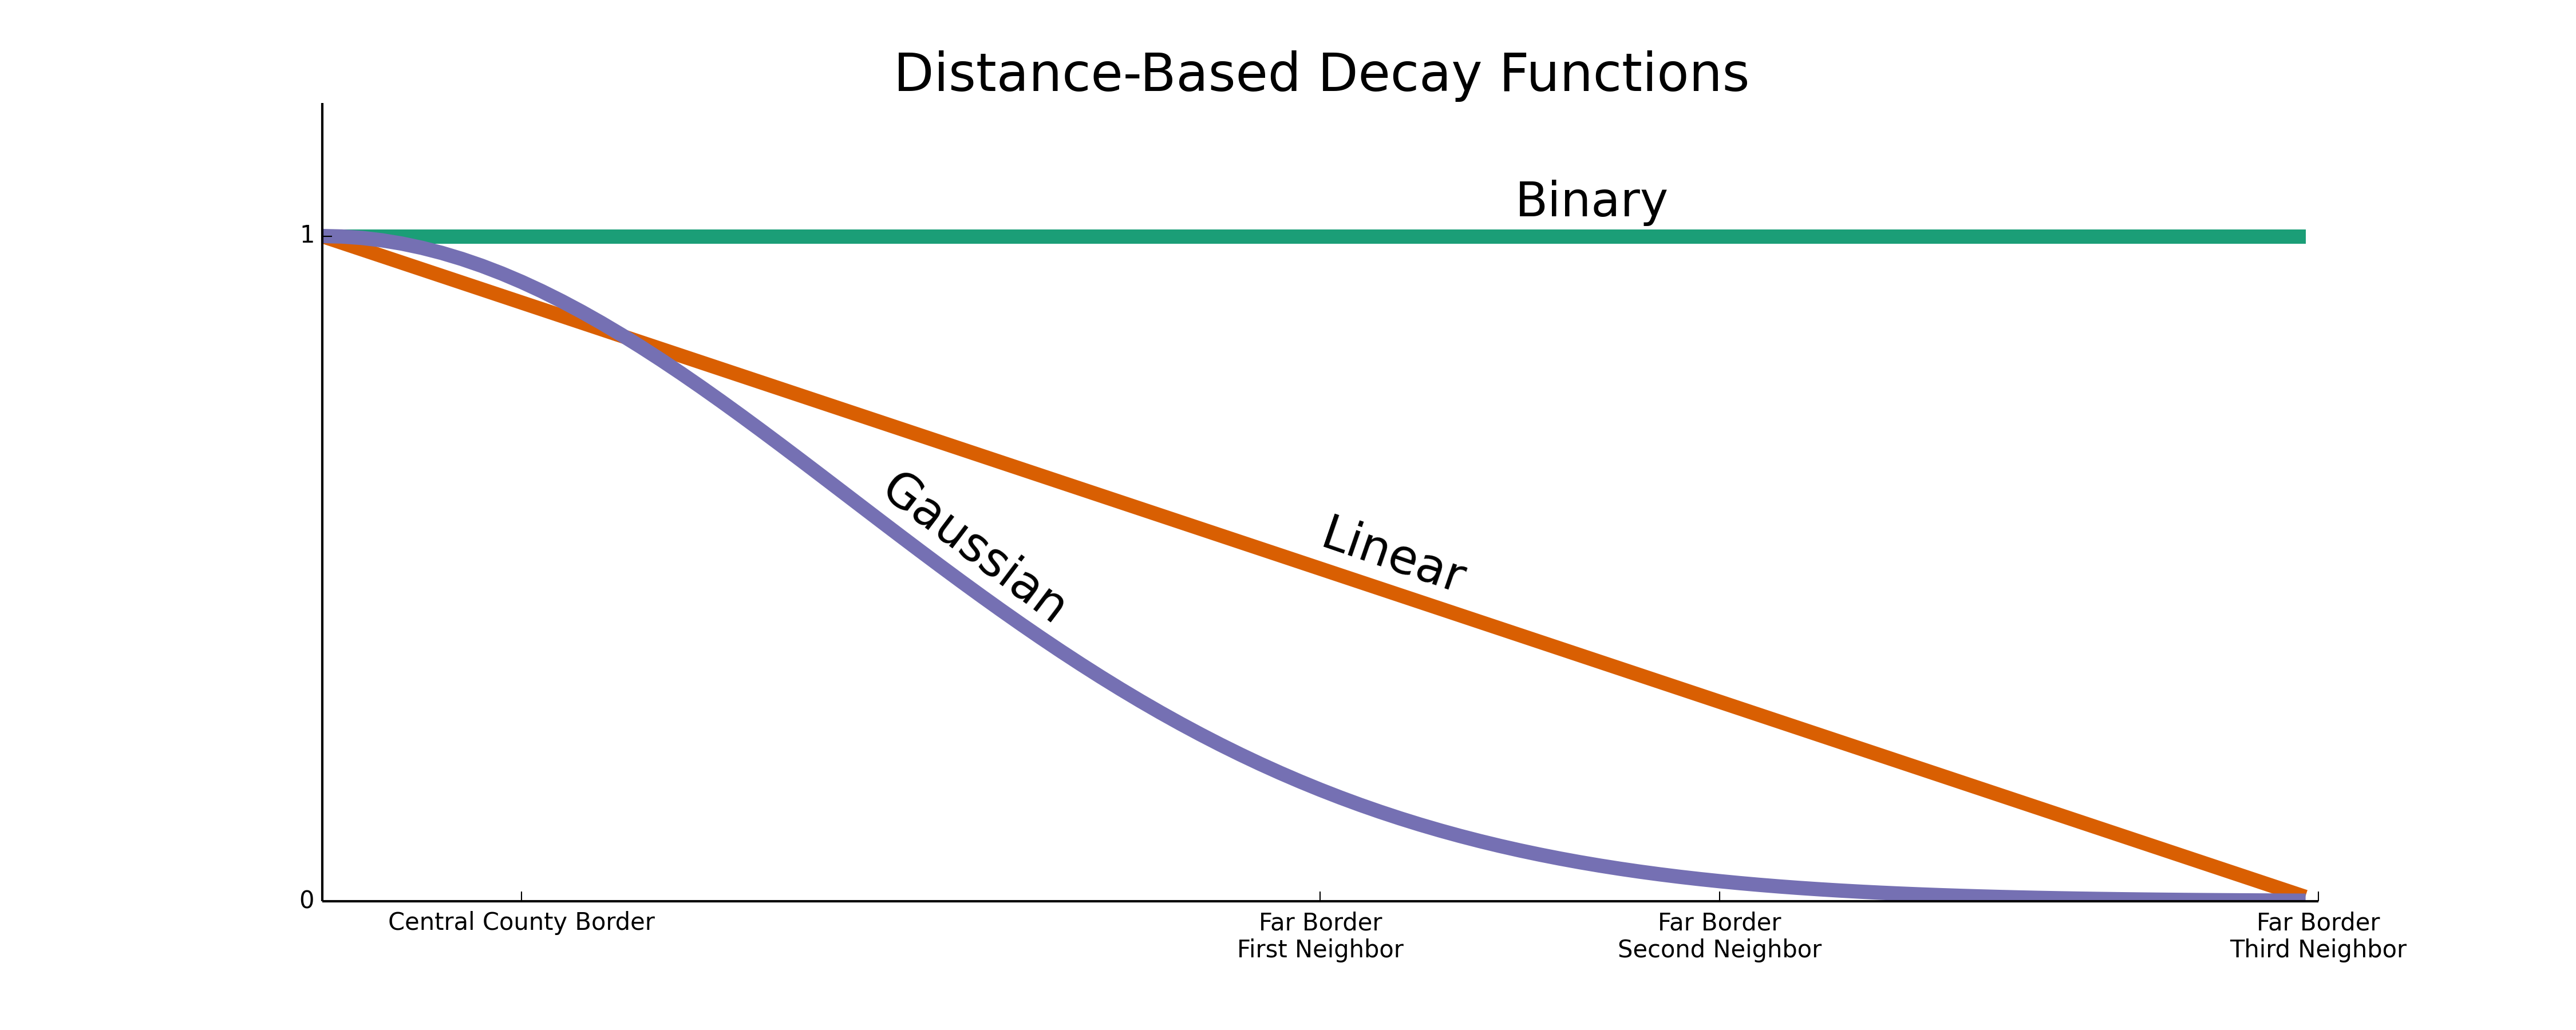
\includegraphics[width=1\textwidth]{figures/decay_curves}
\end{figure}


Given this information, the neighborhoods used to identify hotspots
are defined by the following metrics:
\begin{itemize}
\item Rook Contiguity ($w\_rook$)
\item Queen Contiguity ($w\_queen$)
\item Distance Band - Binary ($w\_db\_b$)
\item Distance Band - Continuous (Inverse Distance Decay;$w\_db\_c$)
\item Kernel (Gaussian Decay;$w\_kern$)
\end{itemize}
Each choice features differing county-specific neighbor counts for
each weight matrix. For example, for rook contiguity ($w\_rook$),
five is the most frequent neighborhood size. This is in sharp contrast
to the kernel matrix ($w\_kern$), which hase only six counties with
a neighborhood of size five. The inconsistent neighborhood size distributions
demonstrates the substantive variation in the definitions employed
by each weight matrix and the reason for sensitivity to neighborhood
definition.


\subsubsection{Local Indicators of Spatial Autocorrelation}

There are two primary measures used to establish spatial clustering
for each weigh matrix/year combination. LMI measures the global spatial
autocorrelation in an attribute $y$ over a given neighborhood. Equation
\ref{alg:Local-Moran's-I} is calculated for each county, $i$. LMI
permits a kind of topological view of autocorrelation. Just as providing
a single moment of a vector of values masks other distributional characteristics
of the data, providing only a single global parameter for spatial
association masks regional dynamics. LMI reveals these dynamics by
providing values for each spatial observation (e.g. county), thereby
enabling the analyst to take note of patterns (e.g. fiscal clusters).
LMI returns high values for a county when it is surrounded by\emph{
similar} values, and it returns low values when it is surrounded by\emph{
disimilar} values (Figure \ref{fig:LMI-Values}).

\begin{model}
\caption{Local Moran's I (LMI)\label{alg:Local-Moran's-I}}


\vspace{10bp}


$$I_i=\frac{\sum_j z_i w_{i,j} z_j}{\sum_i z_i^2}=\frac{\sum_j (y_i-\bar y)w_{i,j}(y_j-\bar y)}{\sum_i(y_i-\bar y)^2}$$
\end{model}


\begin{figure}
\caption[Local Moran's I Values]{Interpretation of Local Moran's I Values\label{fig:LMI-Values}}


\centering{}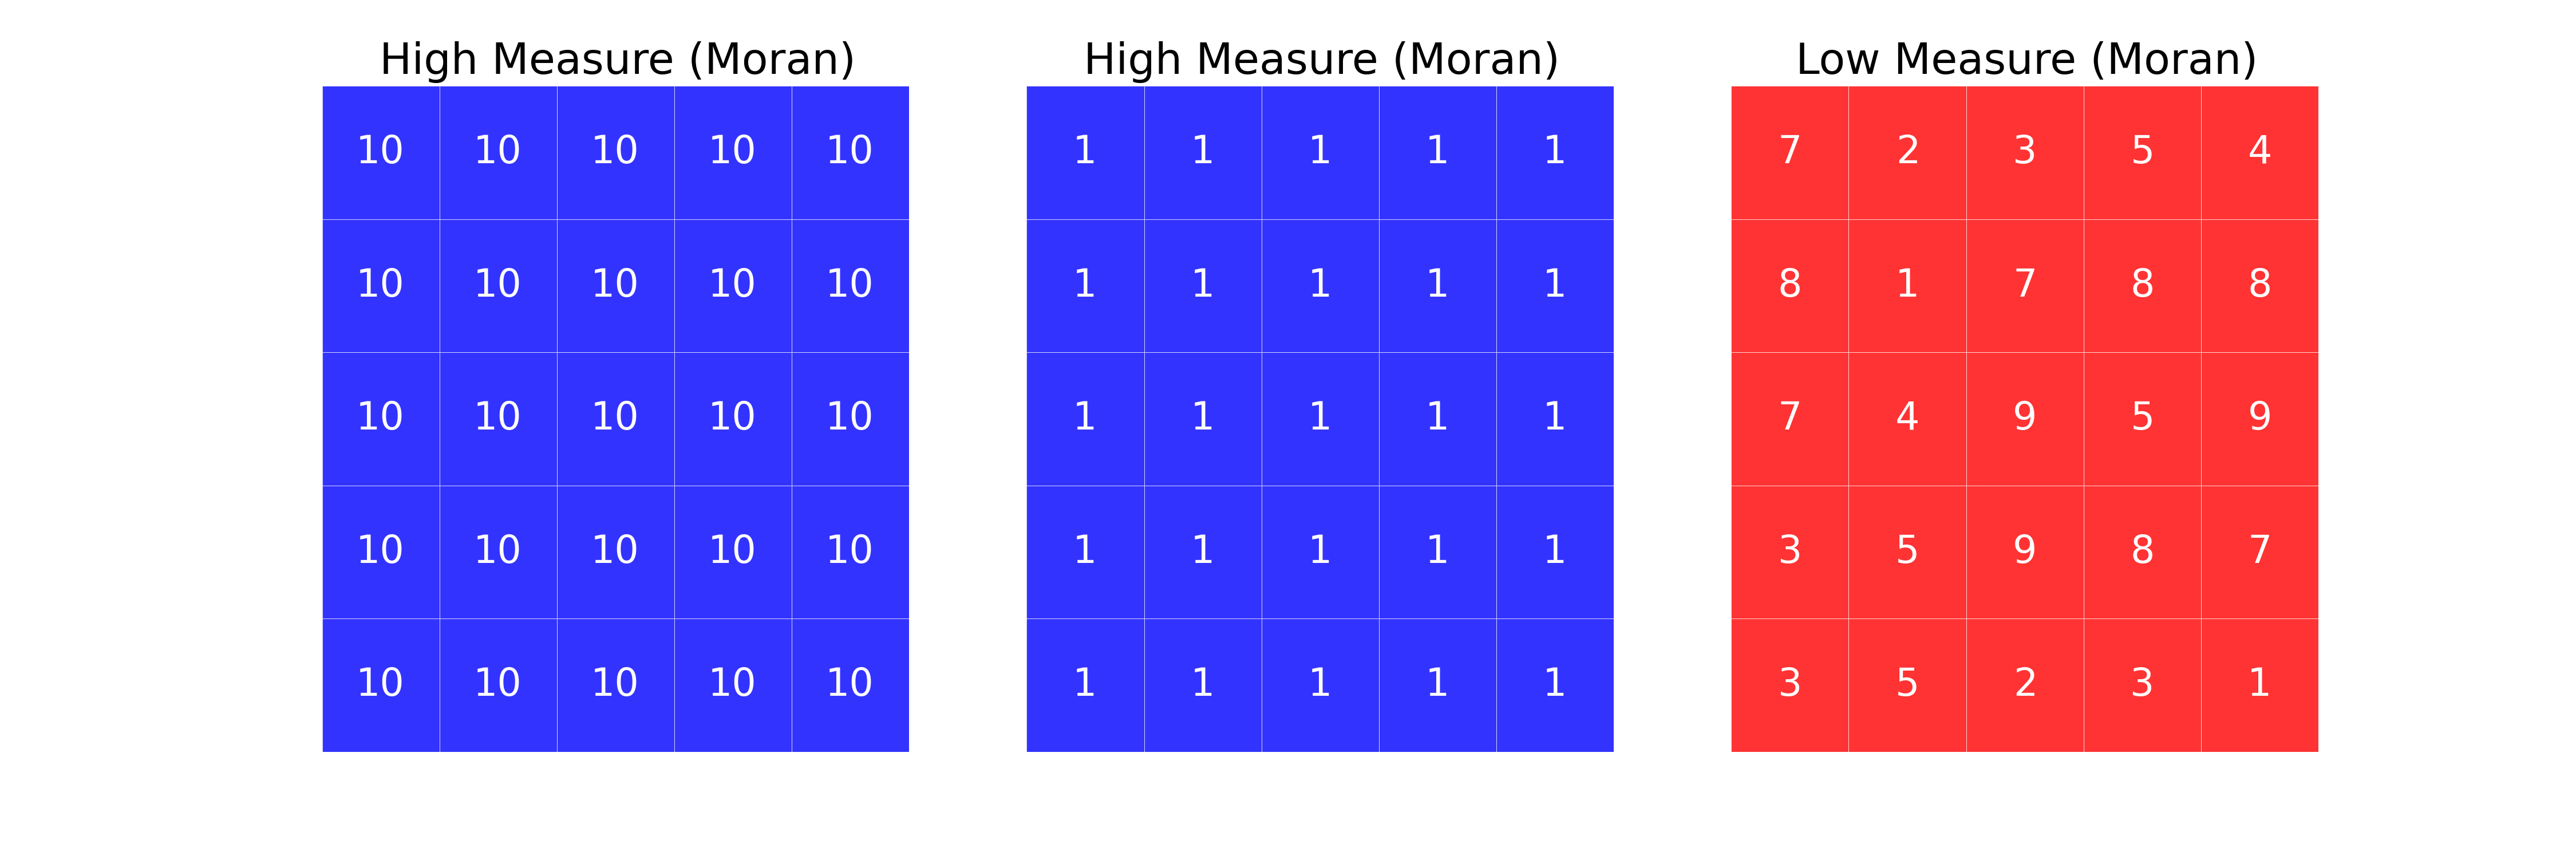
\includegraphics[width=1\textwidth]{figures/Moran_colors}
\end{figure}


As noted by Anselin\citep{Anselin1995}, the interpretation of LMI
is insufficient for a comprehensive knowledge of the clustering behavior
of spatially related activities. It can provide an analyst with knowledge
of the existence of clusters, but it does not provide information
about the type of clustering. In this regard, GOG (Equation \ref{alg:Getis-Ord-G})
is a natural complement. It is also calculated for each spatial feature
(e.g. county). In contrast to LMI, GOG returns high values when\emph{
high} values are clustered and low values when\emph{ low} values are
clustered (Figure \ref{fig:GOG-Values}).

\begin{model}
\caption{Getis \& Ord's G{*} (GOG)\label{alg:Getis-Ord-G}}


\vspace{10bp}


$$G_i(d)=\frac{\sum_j w_{i,j} (d) y_j - W_i\bar y(i)}{s(i)\{[(n-1) S_{1i} - W_i^2]/(n-2)\}^{(1/2)}},j\neq i$$
\end{model}


\begin{figure}
\caption[Getis \& Ord's G{*} Values]{Interpretation of Getis \& Ord's G{*} Values\label{fig:GOG-Values}}


\centering{}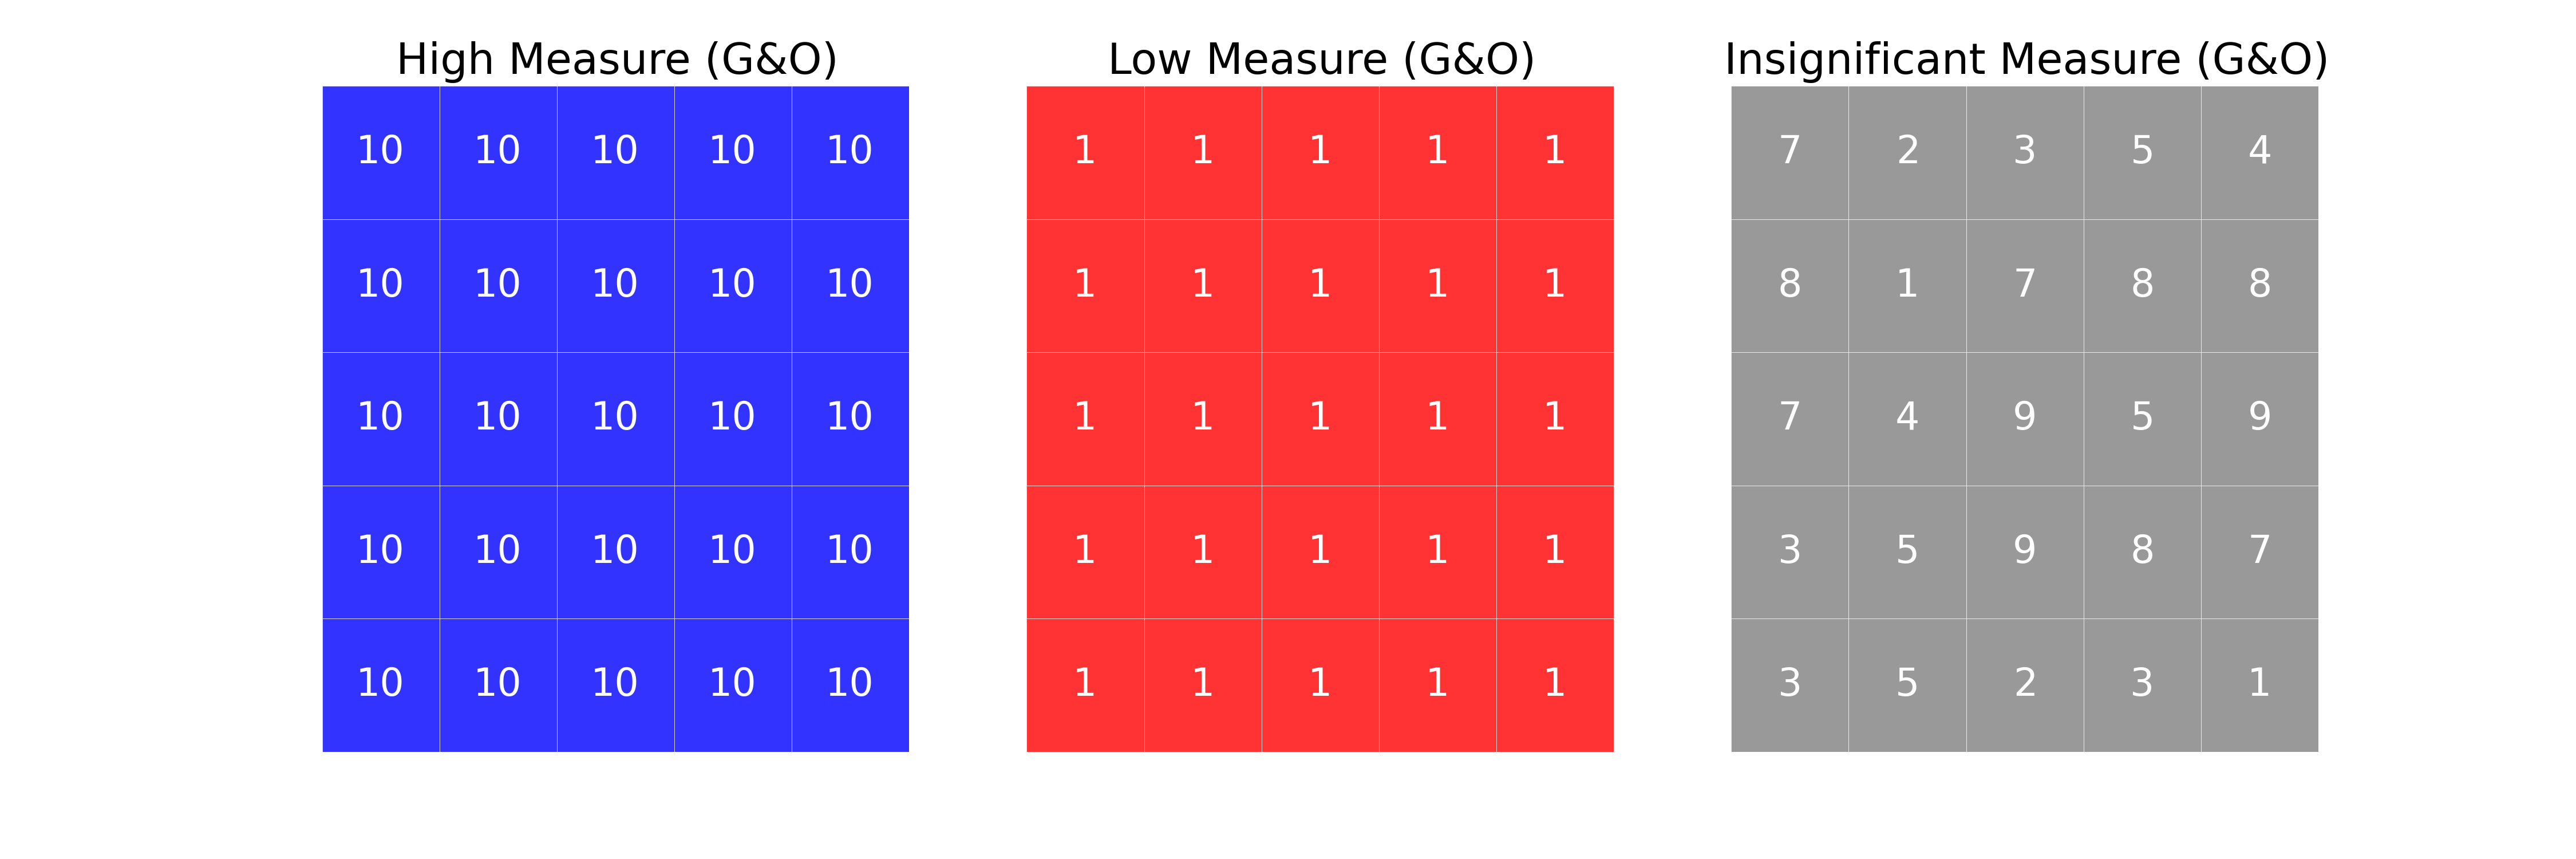
\includegraphics[width=1\textwidth]{figures/GO_colors}
\end{figure}


If one were to rely solely on LMI, the clustering of low revenue capacity
would be indistinguishable from the clustering of high revenue capacity.
If one were to rely solely on GOG, it would not be possible to detect
unusual patterns of discontinuity.\footnote{Unusual patterns would be those discontinuities that were beyond those
which would occur with a random shuffling of values. In other words,
they would be systemic patterns of disimilarity, also known as negative
spatial autocorrelation.} This would render the detection of local anomolies more difficult,
and in turn, the identification of spatial non-stationarity.\footnote{Stationarity is the same concept in a spatial context as it is the
more widespread temporal context. In time series, the joint distribution
of observations must be invariant to a time shift to be considered
strictly stationary.
\begin{quote}
``A time series ${r_t}$ is said to be\emph{ strictly stationary}
if the joint distribution of $(r_{t_1}, ... , r_{t_k})$ is identical
to that of $(r_{t_1 + t}, ... , r_{t_k + t})$ for all $t$, where
$k$ is an arbitrary positive integer and $(t_1, ... ,t_k)$ is a
collection of $k$ positive integers.''
\end{quote}
Weak stationarity just requires that the mean of the reference observation
and the covariance between the reference and a lag of arbitrary size
must be invariant to a time shift. In effect, the observations share
a common mean, and there is some fixed amount of noise.
\begin{quotation}
``A time series ${r_t}$ is\emph{ weakly stationary} if (a) $E(r_t) =\mu$,
which is a constant, and (b) $\mathrm{Cov}(r_t,r_{t-l})=\gamma_l$,
which only depends on $l$.''\citep{Tsay2005}
\end{quotation}
One may think of spatial stationarity in the same way, accept that
lags are not uni-directional as in the time series case. Rather, lags
extend in all directions. In a time series, the observation in the
preceding time period is a first order temporal lag. In a neighborhood
defined by queen contiguity (see Subsection \ref{sub:Weight-Matrices}),
all of the jurisdictions that touch the primary jurisdiction are first
order spatial lags.} Therefore, to gain a complete picture of spatial patterns in revenue
yield and capacity, we must use both LMI and GOG.

The spatio-temporal plots below display spatial clustering activity
over time for each weight matrix. The first collection (Figure \ref{fig:LMI-Plots})
features clustering as a measured by LMI while the second (Figure
\ref{fig:GOG-Plots}) features GOG. In both collections, the first
plot matrix displays clustering of revenue yield (per capita revenue)
and revenue capacity (per capita annual payroll). While the intensity
of clustering does vary to some extent across different weight matrices
(as indicated by varying color intensity), the general patterns persist.

\begin{figure}
\caption{Spatio-Temporal Plots - Local Moran's I\label{fig:LMI-Plots}}


\begin{centering}
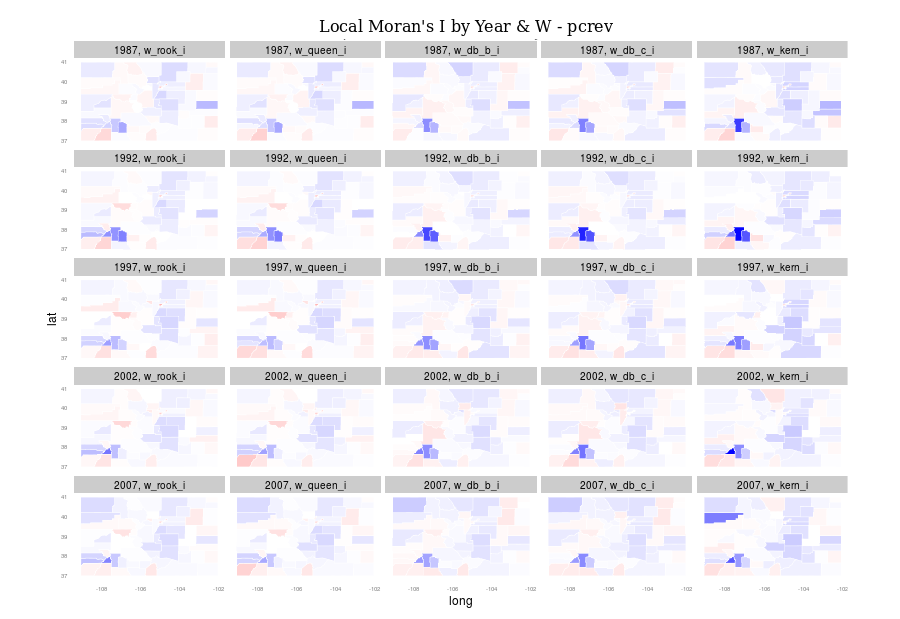
\includegraphics[width=1\textwidth]{figures/moranIPlot_nt}
\par\end{centering}

\centering{}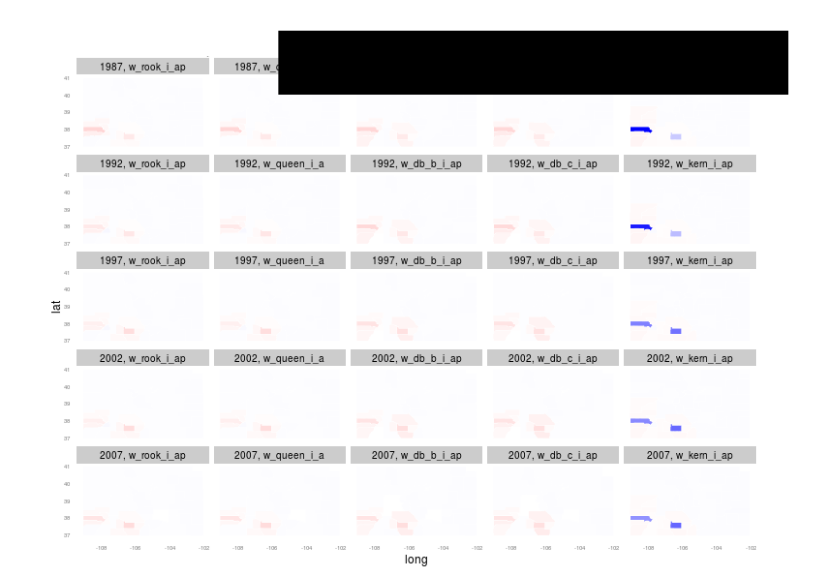
\includegraphics[width=1\textwidth]{figures/Mi_plot_ap_nt}
\end{figure}


\begin{figure}
\caption{Spatio-Temporal Plots - Getis \& Ord's G{*}\label{fig:GOG-Plots}}


\begin{centering}
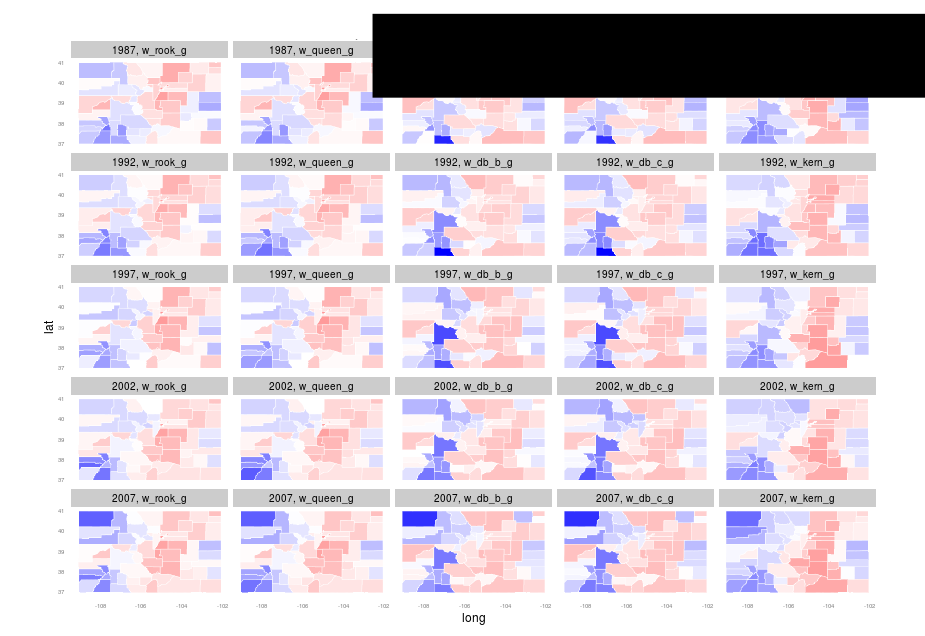
\includegraphics[width=1\textwidth]{figures/goGPlot_nt}
\par\end{centering}

\centering{}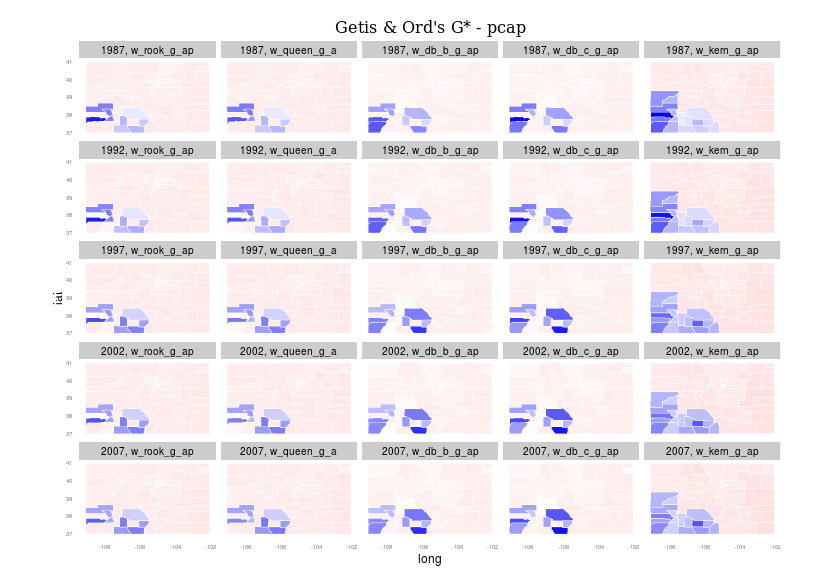
\includegraphics[width=1\textwidth]{figures/GO_plot_ap_nt}
\end{figure}


Not only does revenue yield clustering occur, the extent of the clustering
changes over time. Furthermore, upon closer examination of the data,
three main properties stand out:
\begin{enumerate}
\item Variation is substantially higher in GOG, which indicates relative
consistency in clustering activity, with larger variation in the magnitude
of clustering values. This could mean correlated revenue capacity
shifts across multiple counties within given neighborhoods.
\item Variation is generally more substantial in the higher values for both
statistics. For LMI, this indicates varying intensity of spatial association
amongst similar values. For GOG, this indicates low capacity counties
are more tightly coupled than high capacity counties.
\item Central tendency generally leans right of zero for LMI, and left of
zero for GOG. This suggests a tendency towards the existence of spatial
clustering, but this clustering occurs more often among low capacity
jurisdictions.
\end{enumerate}
\begin{figure}
\caption[LISA Kernel Densities]{Kernel Density Estimates of Year-Specific LISA Values for Revenue
Yield\label{fig:Kernel-LISA}}


These kernel density estimates capture the same information as the
spatio-temporal plots in Figure\ref{fig:LMI-Plots} and Figure\ref{fig:GOG-Plots}.
Instead of displaying the values by county, however, the values for
all counties for a given year are captured in each estimate. The plots
in the left column (with the$_i$ suffix) capture LMI estimates while
the plots in the right column (with the$_g$ suffix) capture GOG estimates.
The weight matrices used are apparent from the labeling. For example,
in the left plot in the first row, each kernel density estimate captures
Local Moran's I values for revenue yield in each year captured (1987,
1992, 1997, 2002, 2007).
\end{figure}



\section{Do TELs Depress Revenue Yield and Capacity?}

Globally consistent trends in clustering are far from clear in the
figures above, but it is clear that there exists variation in the
intensity of clustering as time passes. Extracting the marginal effect
of COTEL intensity requires econometric exploration. In this analysis,
we employ three approaches to explore this impact on measures of both
revenue yield (per capita revenue; $pcrev$) and fiscal capacity (per
capita annual payroll; $pcap$).


\subsection{Modeling Approaches}
\begin{description}
\item [{Pooled~Ordinary~Least~Squares}] estimation serves as the baseline
specification. It is primarily an exploratory modeling exercise to
place the integration of spatial and temporal dependency in context.
Two models, with per capita revenue and per capita annual payroll,
the primary dependents, are evaluated. Furthermore, given the absence
of an explicitly modeled spatial dependency structure, the pooled
OLS approach facilitates the exploration of COTEL intensity impact
on the LISAs defined above. The LISA subset of models use each combination
of LISA measure, fiscal indicator, and weight matrix as the dependent
variable. For example, one dependent ($w\_rook\_i$) will be the LMI
score for per capita revenue, as calculated with rook contiguity.
Dependents capturing annual payroll include an extension:$\_ap$.
The sister dependent variable to $w\_rook\_i$ is $w\_rook\_i\_ap$.
There are two LISAs (LMI and GOG), two fiscal indicators (per capita
revenue and per capita annual payroll), and five weight matrix definitions
(see Subsection WMATRIX). Therefore, there are 20 LISA models.
\item [{Repeated~Cross-Sectional~Spatial~Lag}] estimation provides year-specific
assessments of COTEL intensity impact while incorporating the fiscal
behavior of the local neighborhood. All of these models are evaluated
with the rook contiguity weight matrix ($w\_rook$). The decision
to select one weight matrix for presentation is a function of two
factors. First, the trends revealed by the analysis are generally
insensitive to the choice of weight matrix. Second, presentation of
all weight matrices is likely to suffer from diminishing returns while
simultaneously inhibiting the central message. In general, this series
of models provides some sense of temporal variation over time. There
are two fiscal indicators (per capita revenue and per capita annual
payroll) and 17 years (1993-2009), leading to a total of 34 models.
\item [{Fixed~Effect~Panel}] estimation does not contain a spatial component,
but it does enable us to incorporate county-level unobservable characteristics
(albeit suboptimally). This basically trades one specification element,
spatial autoregression, for another, capture of county-specific factors
that do not explicitly enter the model. The approach provides a cleaner
view of TEL impacts than cross-sectional analysis because the fixed
effects shift the focus to within county deviations. Two of these
models are run, one for each dependent: $pcrev$ and $pcap$.
\end{description}

\subsubsection{Econometrics as Observation\label{sub:Econometrics-as-Observation}}

In total, there are 58 models that will be presented. One would be
well within the bounds of reasonableness to ask why an analyst would
even bother to attempt presentations of so many. The answer is that
this inquiry seeks to partially address a certain type of estimating
uncertainty. When estimating the parameters of an economic process,
the precise nature of what we are estimating is somewhat unclear.
\begin{quotation}
``Haavelmo distinguishes between\emph{ autonomous} relations, which
are invariant to a wide range of interventions, and {[}...{]}\emph{
confluent} relations, which are the result of (complex) interactions
of autonomous relations. Confluent relations may appear stable until
subjected to interventions.''\citep{Hoover1994}
\end{quotation}
We may think of the autonomous relations as those which bind the components
of the true, underlying data generating process. We know that, for
example, the volume of a gas is proportional to its temperature, which
is just a measure of the kinetic energy in the gas. This is a natural
linkage, in the sense that it is always true, everywhere. This is
an autonomous relation. When we seek to measure such a phenomenon,
however, one must worry about confluent relations. For example, we
will not observe the natural linkage between temperature and volume
if the volume is somehow constrained by another variable in the system.
This would produce variation in our estimates, even if no such variation
exists in the underlying data generating process.

Since we have no validation mechanism that reveals the data generating
process\footnote{If we did, of what value would estimation be?},
we cannot know if we are actually observing an autonomous or confluent
relation. Consequently, Hoover suggests that we must assume all of
our observations are confluent interactions between the more conceptually
atomistic autonomous relations. The question remains, what is the
appropriate mitigation strategy?

First and foremost, we must recognize that each econometric strategy
we may employ has its failings. For example, fixed effect estimation
is useful for capturing the aggregate impact of group-specific characteristics,
but by failing to identify the characteristics covered by the fixed
effect explicitly it creates challenges in exploring the specific
nature of these impacts. Just as a sample drawn from a population
provides a specific view of the population that does not capture its
full variety, the model an analyst chooses to employ captures a particular
view of that sample. That view is a function of both the strengths
and weaknesses of the modeling approach and the specification evaluated
by the analyst.
\begin{quotation}
``Economists customarily speak of these {[}models{]} as 'good', 'bad',
'valid' and 'invalid'. Given the distinction between the data-generating
process and confluent relations, it would be more to the point to\emph{
think of these econometric calculations themselves as observations
of the confluent relations}. As such they may be illuminating or useful
or neither, but not valid or invalid.''\citep{Hoover1994} (emphasis
added)
\end{quotation}
Conceiving of econometric calculations as observations of the underlying
interplay between the components of the true data generating process
shifts the focus away from the identification of precise estimation
of an effect\emph{, if one seeks to flesh out the dynamics needed
to shape a paradigm of thinking about a given phenomenon.} To the
extent that the analysis presented here is largely an effort to open
the study of TELs to a broader array of potentially confounding elements,
the analysis is more about the establishment of directional action.

In this light, an ensemble approach like that used here is useful.
Instead of precision, we are concerned with agreement. The more observations
(that is, econometric calculations) that support the direction of
impact for a given variable, the higher the degree of confidence we
can ascribe to the our proposed view of the world.


\subsection{Members of the Regressor Set}

The independent control variables seek to capture changing dynamics
in the economic and demographic conditions by county. State level
indicators are also included to provide macro-level context, as are
our primary variables of interest (those capturing COTEL impact).
\begin{description}
\item [{Gross~State~Product~($gsp$)}] provides a measure of statewide
economic activity. It is intended to capture some measure of resources
available to the state in a given year. It is omitted in the repeated
cross-sectional models, because it does not vary across counties within
a single year.
\item [{Lagged~Population~Growth~($lpop\_growth$)}] provides a measure
of public demand for services and housing. With respect to the former,
demand for services (a.k.a. expenditure need) determines the level
of revenue required in a given year. With respect to the latter, population
growth drives the demand for housing, which in turn drives up prices
and the overall value of the revenue base.
\item [{State~Level~Unemployment~Rate~($st\_unempr$)}] is a business
cycle indicator. Economic downturns have dynamic consequences for
jurisdictions subject to TABOR.\citep{LegStaff2003} Specifically,
downturns increase the likelihood of the revenue yield failing to
reach the growth ceiling imposed by TABOR/SLPTR. The consequence is
a permanently lowered revenue baseline in the absence of a local override.
\item [{Housing~Permits~per~Unit~Housing~($permit\_rate$)}] is related
to population growth, but it provides a more direct, concurrent measure
for housing market pressures. More importantly, it captures the TABOR
growth factor (new construction) in a straightforward way.
\item [{Vacancy~Rate~($vac\_rate$)}] is the most direct measure of housing
demand. There are reasons for both the population growth and permit
rate indicators to separate from stock utilization. For example, population
growth may be accompanied by increases in household size and permit
rates may increase due to developer forecasting assumptions. Neither
separation is possible with the vacancy rate.
\item [{Total~Revenue~From~All~Governments~($all\_gov\_rev$)}] captures
the cumulative receipts for all governments in the county. It is meant
to give a sense of the total volume of public resources available
in the county. (Recall that $pcrev$ captures only county government
receipts per capita.)
\item [{County~Proportion~of~Total~Revenue~From~All~Governments~($cty\_rev\_prop$)}] captures
the proportion of cumulative receipts for all governments in the county
that is collected by the county government. County governments are
an unambiguously important component of fiscal operations, but the
magnitude of that importance can vary across counties. This measure
also speaks to the ability of other governmental entities to pick
up the slack when counties are constrained.
\end{description}

\subsubsection{Variable of Interest}
\begin{description}
\item [{Ratio~of~Residential~to~Non-Residential~Assessment~Value~($prop\_ratio$)}] captures
the county-specific value of the measurement used to set statewide
assessment rates pursuant to the Gallagher Amendment. It is one of
our primary variables of interest.
\item [{Cumulative~Impact~of~TABOR~and~SLPTR~($intensity\_stock$)}] is
another primary variable of interest. It captures the extent to which
TABOR and SLPTR limit the revenue yield for a county to reach its
potential.
\end{description}
\begin{figure}


\caption{Regressor Correlation Plot\label{fig:Correlation-Plot-Rev}}


\begin{centering}
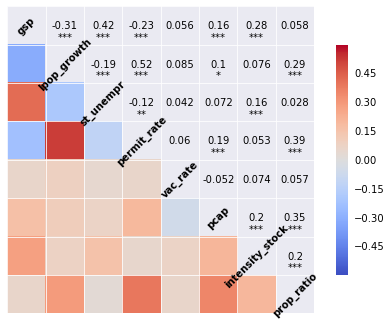
\includegraphics[width=0.85\textwidth]{figures/converge_indep_corrplot}
\par\end{centering}

\end{figure}


The fiscal yield models regress fiscal yield ($pcrev$) on all of
the above regressors\emph{ and fiscal capacity} ($pcap$). The fiscal
capacity models, on the other hand, only include the above regressors.
Fiscal yield does not enter the fiscal capacity models. Note that
all dollar amounts have been adjusted to reflect 2009\$.


\subsection{Results}

Clearly, there are challenges associated with the presentation of
58 models. As mentioned above, however, our overarching concern is
consistency. To what extent do the models tell the same story. With
this in mind, we are afforded some flexibility in presentation. A
graphical approach is taken here. Furthermore, a summary view of the
LISA models is provided, each view of which shares averages of coefficient
estimates, p-values, and model fit for all five weight matrices presented.
In all of the visualizations that follow, three interpretations apply:
\begin{enumerate}
\item Coefficient estimates are represented by the y-axis value;
\item $p$-values are represented by color of the bubble\footnote{A diverging color scale is used.$p$-values below 0.1 are a shade
of blue, while values above 0.1 are a shade of red.}; and,
\item Model fit ($R^2$) is represented by the size of the bubble.
\end{enumerate}

\subsubsection{Baseline Estimation with Pooled Ordinary Least Squares}

As will become apparent, the pooled OLS models provide a view of a
counterintuitive, yet relatively consistent, narrative. While the
COTEL intensity measure ($intensity\_stock$) has the expected negative
and statistically significant effect on revenue yield ($pcrev$),
higher values of the intensity measure are consistently associated
with higher levels of fiscal capacity ($pcap$). This is a curious
result that directly challenges the notion that COTELs limit the fiscal
capacity of a given county. Furthermore, the same revenue yield relationship
holds for the ratio of residential and non-residential property ($prop\_ratio$)
used to capture the impact of the Gallagher Amendment (the Gallagher
Ratio). Again, higher relative amounts of residential property are
associated with lower revenue yields. This accords with intuition
to the extent that GA is designed to limit residential property tax
liability. Fiscal capacity, on the other hand, is higher in counties
which have higher relative levels of residential property in the assessment
base.

\begin{figure}


\caption[Pooled OLS Results]{Pooled OLS Results - Fiscal Capacity (\emph{left}) \& Revenue Yield
(\emph{right})\label{fig:Pooled-OLS-Results}}


\centering{}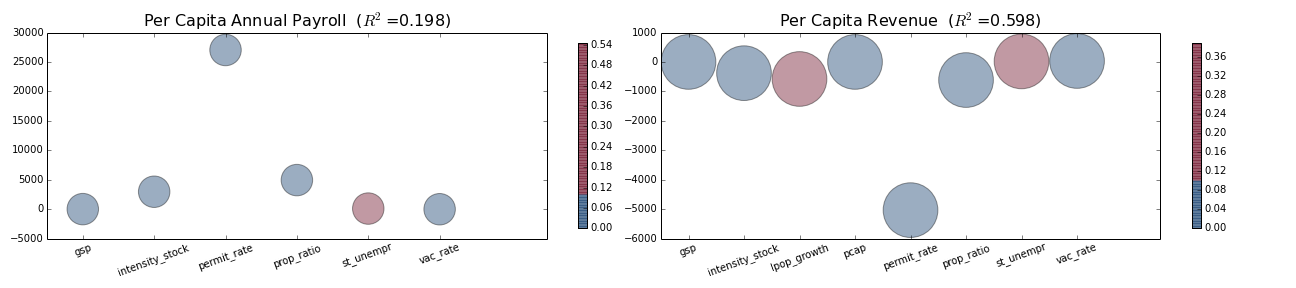
\includegraphics[width=1\textwidth]{figures/converge_pooled_ols}
\end{figure}


Note also the large disparity in model fit across the two models.
This is a persistent character of this analysis - all of the revenue
yield models explain a larger portion of the variance than do their
fiscal capacity counterparts. This is perhaps unsurprising. The impact
of institutions and economic changes on revenue yield is much more
direct than is the impact on fiscal capacity. Complete identification
of this indirect linkage can be pursued in future research.


\subsubsection{Evaluating the Impact on Fiscal Clustering with Local Indicators
of Spatial Autocorrelation (LISAs)}

Using the LISAs as dependents provides some notion of how the variables
in the model impact spatial clustering of revenue yield and fiscal
capacity. Counties experiencing higher levels of COTEL intensity are
expected to converge in the revenue yield and fiscal capacity incomes.
In effect, the COTELs are expected to retard their revenue growth,
which will create a wedge between constrained and unconstrained counties.
It has already been shown that spatial clustering of fiscal behavior
occurs, so this wedge is expected to be spatiall relevant. The visualization
of these results employs averages across the five weight matrices
used in this analysis (see Subsecton\ref{sub:Weight-Matrices}). Again,
this is to limit the sensitivity of interpretation to choice of the
local neighborhood,$W$.

To reiterate, high values of LMI indicate the clustering of similar
values, while low values indicate the clustering of disimilar values.
In other words, high values of LMI can indicate the presence of a
local neighborhood of counties characterized by either high revenue
yield/fiscal capacity or low revenue yield/fiscal capacity. In contrast,
high values of GOG indicate clustering of high values, while low values
of GOG indicate clustering of low values. Thus, LMI reveals more about
the strength of clustering while GOG reveals more about the type of
clustering.

\begin{figure}
\caption[LISA Results]{LISA Results - Revenue Yield (\emph{left}) \& Fiscal Capacity (\emph{right})\label{fig:LISA-Results}}


\centering{}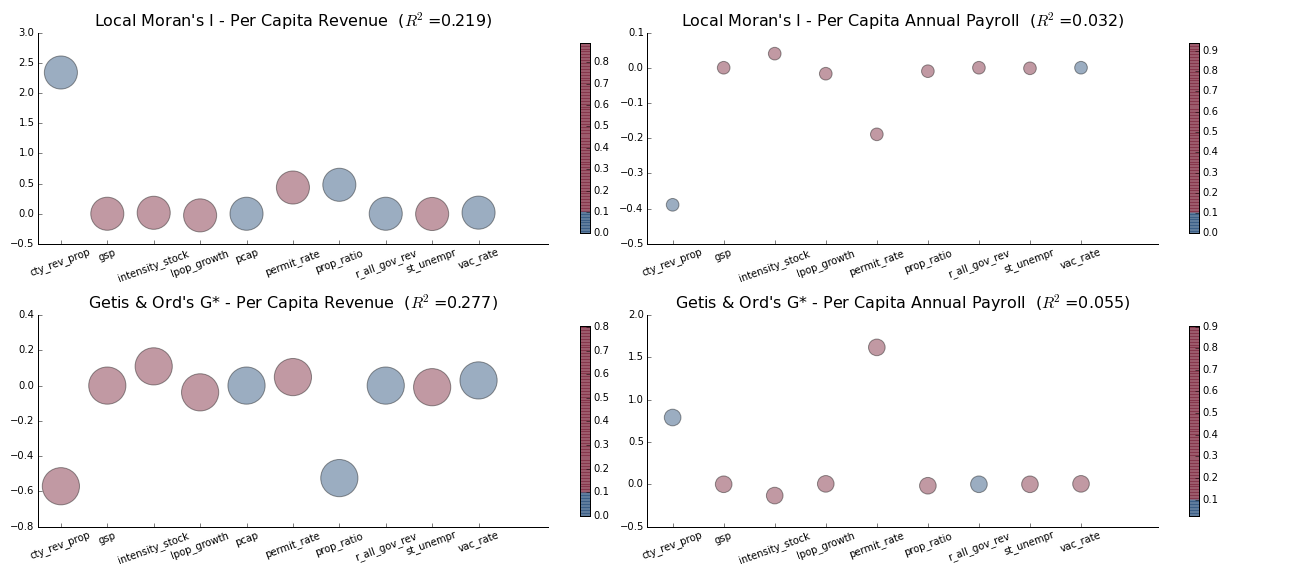
\includegraphics[width=1\textwidth]{figures/converge_LISAs}
\end{figure}


\emph{Note: Need to place these results in context. What is the range
of clustering values? What is a significant movement?}

When controlling for other factors, COTEL intensity ($intensity\_stock$)
has very limited impact on the clustering of revenue yield ($pcrev$).
Said differently, if a county is highly constrained, the constraint
is not a significant driver of the clustering that already exists.
This is interesting because one could reasonably expect that the inflexibility
of achievable expenditures in the constrained county would force convergence
in fiscal behavior, thereby taking jurisdictional idiosyncrasies out
of the siting equation and reinforcing similar revenue preferences
in the local neighborhood. It is possible that collaborative efforts
in the local neighborhood to provide wide area services free up enough
revenue to still allow for some base level of distinction. In any
event, the only reasonably clear impact of COTEL intensity is a negative
association with fiscal capacity ($pcap$) clustering values (GOG),
which indicates that higher levels of COTEL constraints are related
to clustering of low values of fiscal capacity. This accords with
the hypothesis that COTELs ultimately limit fiscal capacity for low-income
jurisdictions.

On the other hand, the Gallagher Ratio ($prop\_ratio$) behaves precisely
as we would expect from a revenue yield perspective. Insofar as it
increases the strength of clustering (higher values of LMI) and decreases
the values assoicated with said clustering (low values of GOG), the
evidence suggests that the measure is a limiting factor on revenue
yield in the local neighborhood. On the fiscal capacity side, the
Gallagher Ratio is neither statistically or substantively relevant.

In both the revenue yield and fiscal capacity models, the model fit
is modest at best (particularly with respect to the latter) and categorically
lower than the fit of any other model considered in this chapter.


\subsubsection{Incorporating the Local Neighborhood with Spatial Lags}

Repeated SLM analysis allows us to incorporate the local neighborhood
explicitly because the spatial lag of the dependent variable is the
weighted average of the dependent variable value in the neighboring
jurisdictions. Evaluating annual cross-sections is useful insofar
as it provides a view of the variation in regressor impact over time,
both in magnitude and significance. The non-trivial downsides are
two-fold:
\begin{enumerate}
\item Repeated cross-sections do not permit control of year-specific factors;
and,
\item To the extent that deBrucing is an ongoing phenomenon, there is temporal
variance in the sample properties. The characteristics, namely the
capacity of COTELs to constrain a given jurisdiction, of the counties
are changing over time.
\end{enumerate}
As a consequence, the technique can only be useful in this context
as a complementary component in a larger analysis.

\begin{figure}


\caption[SLM - Revenue Yield]{Spatial Lag Models by Year - Revenue Yield ($pcrev$)\label{fig:SLM-Rev}}


\begin{centering}
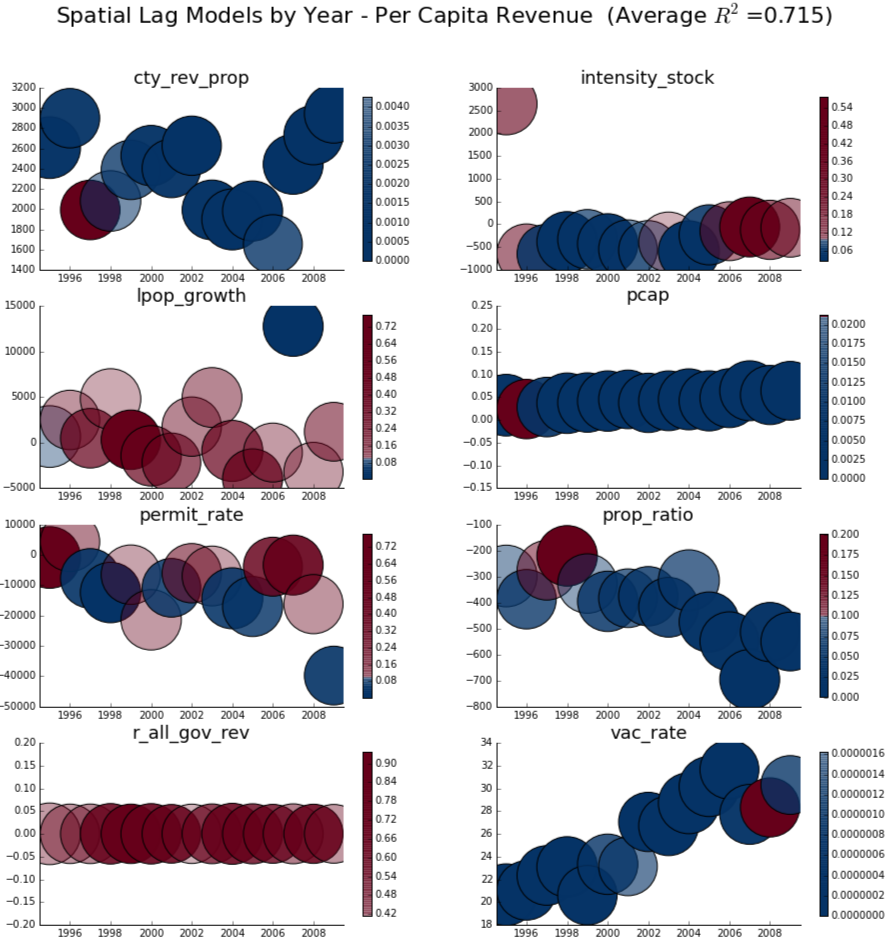
\includegraphics[width=1\textwidth]{figures/converge_slm_rev}
\par\end{centering}

Note: the single red data points in the$pcap$,$prop\_ratio$, and$vac_rate$
subplots are only artifacts of the plotting function. As can be seen
in the color bar, the range of p-values for these variables is entirely
below$p$=0.1. The final version of this graphic will remedy this
issue with post-hoc adjsutment of the an SVG version of the plot.
\end{figure}


With respect to revenue yield, both COTEL intensity ($intensity\_stock$)
and the Gallagher Ratio ($prop\_ratio$) accord with the pooled OLS
results. They both materially decrease the revenue per capita in the
county, even after controlling for the revenue dynamics in the local
neighborhood. In other words, these are reductions over and above
the preferences that may be shared with neighboring jurisdictions.

The interesting dynamic revealed by the repeated cross-sectional approach
is that COTEL intensity appears to get less significant over time,
both in statistical and substantive terms. In contrast, the Gallagher
Ratio is doing precisely the opposite. This could indicate either
a shift in the composition of counties subject to binding COTEL constraints
or a shift in the composition of the property assessment base (or
both).

Evaluating fiscal capacity with the repeated SLM approach reveals
the tenuous nature of any direct connection between our COTEL variables
and per capita annual payroll. COTEL intensity is insignificant in
every single year, while the Gallagher Ratio demonstrates substantial
variation in magnitude and statistical clarity. With respect to the
latter, it is also worth noting that the sign of the Gallagher Ratio
estimate has switched from the pooled OLS run. Finally, even when
controlling for the other factors, the underlying positive relationship
between per capita annual payroll and the Gallagher Ratio.

\begin{figure}


\caption[SLM - Fiscal Capacity]{Spatial Lag Models by Year - Fiscal Capacity\label{fig:SLM-econ}}


\begin{centering}
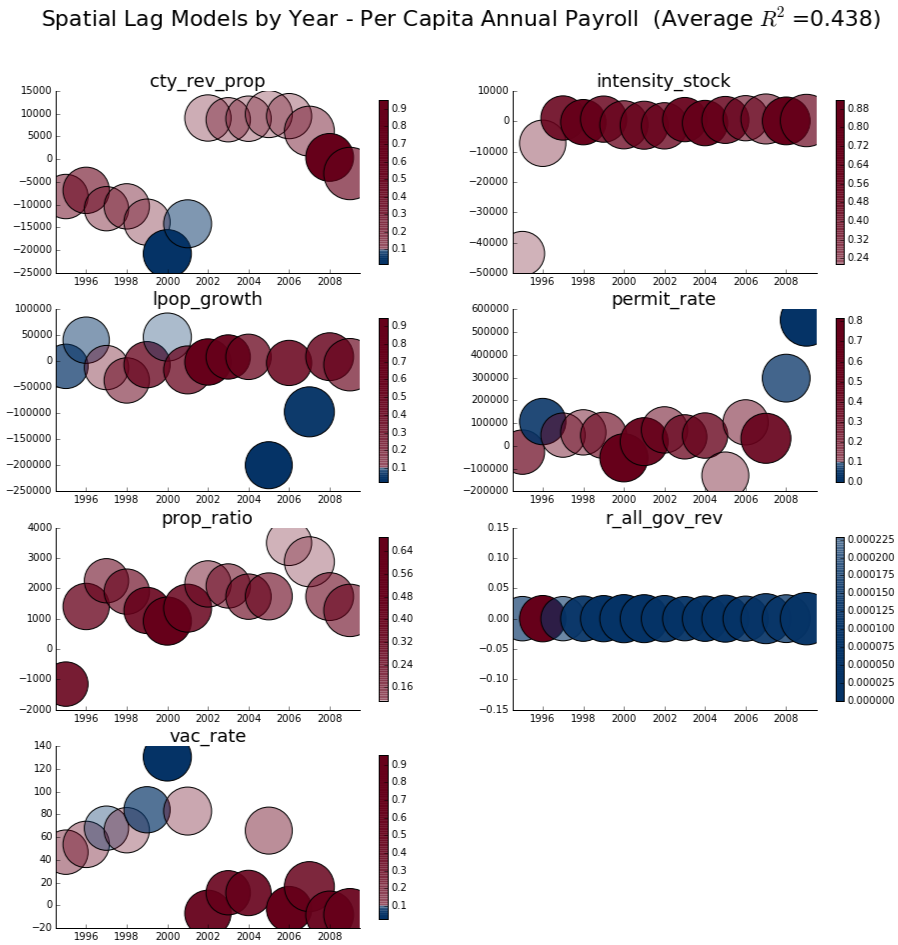
\includegraphics[width=1\textwidth]{figures/converge_slm_econ}
\par\end{centering}

WHY IS THERE A DIP IN 2002? IS IT RECESSION RELATED?
\end{figure}



\subsubsection{Capturing Temporal Dependency with Fixed Effects}

Pivoting from the modeling of spatial to temporal dependency, it is
possible to control for county-specific unobservables that may obscure
the mechanism by which changes in COTEL intensity ($intensity\_stock$)
and the Gallagher Ratio ($prop\_ratio$) effect changes in revenue
yield and fiscal capacity. The panel model results plot for revenue
yield reveals a consistent theme for most variables, although the
permitting rate ($permit\_rate$) sign has switched. Both COTEL intensity
and the Gallagher Ration are modestly depressing forces on revenue
yield in a given county.

\begin{figure}
\caption[Fixed Effect Estimation]{Fixed Effect Model Results - Revenue Yield (\emph{left}) \& Fiscal
Capacity (\emph{right})\label{fig:FE-Results}}


\centering{}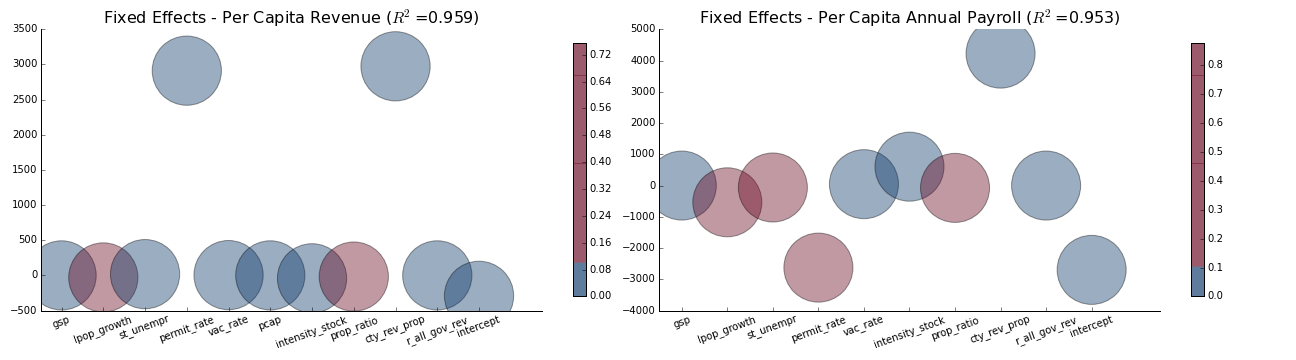
\includegraphics[width=1\textwidth]{figures/converge_fe_panel}
\end{figure}


The raw coefficient estimates are provided in Tables\ref{tab:FE-Rev-Table}
and\ref{tab:FE-Econ-Table} . If the estimates are standardized to
reflect the impact sizes as a multiple of the standard deviation,
a one standard deviation shift in COTEL intensity accounts for a shift
in revenue yield of approximately 4\% of one standard deviation in
revenue yield ($pcrev$). The parallel impact for the Gallagher Ratio
is 9\%. These figures are roughly three times as large as those reported
in the pooled OLS model, and twenty times as large as those reported
in the spatial lag models (on average).\footnote{Note that this is the average response to a shift of a single standard
deviation across the models for all years. Thus, this effect would
not necessarily scale linearly,\emph{even if the impact of a change
in COTEL variables were consistent through the entire range of COTEL
values}.}

\begin{table}


\caption[FE Results - Revenue Yield]{Fixed Effect Estimation - Revenue Yield ($\mathrm{R}^2=.923$)\label{tab:FE-Rev-Table}}


\vspace{10bp}


\begin{centering}
\begin{tabular}{l|r@{\extracolsep{0pt}.}lcc}
Variable & \multicolumn{2}{c}{$\beta$} & $p$-value & S.E.\tabularnewline
\hline 
\hline 
Gross State Product ($gsp$) & 0&001 & 3.112$\times 10^{-05}$ & 0.000\tabularnewline
Lagged Population Growth ($lpop\_growth$) & -151&486 & 5.409$\times 10^{-01}$ & 247.670\tabularnewline
State Unemployment Rate ($st\_unempr$) & 32&103 & 3.194$\times 10^{-07}$ & 6.238\tabularnewline
Housing Permits Rate ($permit\_rate$) & 1883&634 & 1.178$\times 10^{-02}$ & 746.473\tabularnewline
Vacancy Rate ($vac\_rate$) & 6&792 & 5.783$\times 10^{-03}$ & 2.456\tabularnewline
Fiscal Capacity ($pcap$) & 0&040 & 6.414$\times 10^{-17}$ & 0.005\tabularnewline
COTEL Intensity ($intensity\_stock$) & -102&841 & 1.580$\times 10^{-02}$ & 42.539\tabularnewline
Gallagher Ratio ($prop\_ratio$) & -167&069 & 2.137$\times 10^{-02}$ & 72.483\tabularnewline
\end{tabular}
\par\end{centering}

DO TELS REDUCE REV YIELD MORE IN DISTRESSED COUNTIES? MUST BE IN PROPORTIONAL
TERMS
\end{table}


\begin{table}
\caption[FE Results - Fiscal Capacity]{Fixed Effect Estimation - Fiscal Capacity ($\mathrm{R}^2=.947$)\label{tab:FE-Econ-Table}}


\vspace{10bp}


\begin{centering}
\begin{tabular}{l|r@{\extracolsep{0pt}.}lcr@{\extracolsep{0pt}.}l}
Variable & \multicolumn{2}{c}{$\beta$} & $p$-value & S&E.\tabularnewline
\hline 
\hline 
Gross State Product ($gsp$) & 0&028 & 3.807$\times 10^{-72}$ & 0&001\tabularnewline
State Unemployment Rate ($st\_unempr$) & -8&535 & 8.381$\times 10^{-01}$ & 41&753\tabularnewline
Housing Permits Rate ($permit\_rate$) & -6382&604 & 1.949$\times 10^{-01}$ & 4921&187\tabularnewline
Vacancy Rate ($vac\_rate$) & 55&274 & 7.603$\times 10^{-04}$ & 16&367\tabularnewline
COTEL Intensity ($intensity\_stock$) & 1755&172 & 7.435$\times 10^{-10}$ & 282&346\tabularnewline
Gallagher Ratio ($prop\_ratio$) & -576&022 & 2.394$\times 10^{-01}$ & 489&347\tabularnewline
\end{tabular}
\par\end{centering}

TELS ARE ACTUALLY CONSTRAINING THE COUNTIES WITH THE GREATEST GROWTH,
WHICH IS DIFFERENT THAN STRESS INDUCEMENT. ELABORATE

THEY MORE STRONGLY CONSTRAIN RICHER COUNTIES, BUT DON'T NECESSARILY
KILL THEIR CAPACITY TO PRODUCE?

WHAT IS WORSE? POOR ENDOWMENT OR POOR CAPACITY TO GROW REVENUE?

EXHIBIT: SUMMARY TABLE - TEL INTENSITY FOR STRESSED VS NOT STRESSED
COUNTIES
\end{table}


The results of the panel analysis of fiscal capacity do little to
sort out a pattern in the estimates reported in previous models. While
COTEL intensity is still positive and significant once again, the
Gallagher Ratio is now negative. The latter result contrasts sharply
with the pooled OLS and SLM models. This may suggest that the other
models were using the Gallagher Ratio as a proxy for some of the unobserved
characteristics we are now capturing in the fixed effects.


\section{Summary of Findings and Conclusion}

This analysis was designed to evaluate the impact of the cumulative,
composite limit imposed by TABOR and the Statewide Limit on Property
Tax Revenue (a.k.a. COTEL intensity), as well as the Gallagher Amendment,
on two fiscal indicators: revenue yield (revenue per capita) and fiscal
capacity (annual payroll per capita). To pursue this objective, the
analysis employed pooled OLS, spatial lag models, and panel analysis
to identify patterns in the COTEL impacts from a variety of perspectives.
While there was non-trivial variation in the magnitude of impact,
COTELs consistently depressed revenue yields. This accords with intuition,
and empirical exploration has borne this out.

In constrast, the fiscal capacity models consistently explained less
variation relative to revenue yield models, and the impacts of COTELs
were inconclusive across models. The implication is that COTELs do
not have direct impacts on fiscal capacity. Rather, the ultimate impact
is likely a function of how individual counties respond to the constraints
placed on them by statewide COTEL policies.

It should also be noted that the analysis in this paper makes clear
that differential impacts across counties are non-trivial. These disparities
in the impacts of COTELs are drive by dynamic economic characteristics
of each county. Furthermore, the economic circumstances of counties
display spatial dependency, and spatial clustering occurs more strongly
among low revenue/capacity counties. Consequently, policies that depress
revenue yield or fiscal capacity exacerbate this phenomenon. With
respect to revenue yield, it is clear that COTELs do just that. The
impact of COTELs on fiscal capacity, however, warrants greater study.

\clearpage


\chapter{Alteration of Expenditure Patterns\label{chap:Expenditure-Patterns}}


\section{Introduction}

In Chapter\ref{chap:RevYieldCapacity}, the impact of COTELs on the
revenue side of county finance in Colorado was explored. This chapter
focuses on the other side of the equation: expenditure behavior. This
shift in focus is designed to structurally capture the duality of
public finance discussed in Subsection\ref{sub:Duality-in-Public-Finance}.
While popular discourse tends to decouple the two, revenues and expenditures
are instrinsically linked. Each unit of revenue collected by a government
not used to cover the cost of labor is redeployed as some programmatic
output designed to either increase the real income of constituents
or increase their capacity to generate income elsewhere. Even though
the topic of revenue could have consumed the entirety of this dissertation,
recognition of fiscal duality demands some level of balance in topic
selection.

Whereas Chapter \ref{chap:RevYieldCapacity} was concerned with the
general capacity of a county to finance public services, this chapter
begins to explore the specific expenditure choices made in the context
of COTELs and fiscal clustering. In particular, it seeks to understand
whether or not counties that face constraints under the TEL regime
in Colorado make different choices about how to spend public funds
than they otherwise would. Indeed, since we do not observe an alternative
state of the world, such a question raises certain difficulties. The
chief obstacle is the establishment of an artifical, yet defensible,
counterfactual scenario. The analysis that follows leans on basic
tools of machine learning to construct such a scenario. In so doing,
this chapter serves two purposes. First and foremost, it sheds light
on the expenditure side impact of COTELs. Second, it suggests that
students of public finance can learn from the methods of others, which
sometimes have favorable characteristics that help to mitigate deficiencies
in more conventional methods. In general, we should seek to employ
complementary (but not redundant) tools whenever possible, even if
they are unconventional from the field's perspective. As discussed
in Subsection \ref{sub:Econometrics-as-Observation}, consistent results
from a variety of calculations lends credibility to the analysis.


\section{Why does a Shift in Expenditure Patterns Matter?}

In\emph{The Pure Theory of Public Expenditure}\citep{Samuelson1954},
Paul Sameulson evaluated the implications of the joint consumption
of public goods. This feature of public goods separates them from
private goods along one very important dimension: the feasibility
of preference revelation. Without the ability to determine what an
individual would pay for the marginal unit of public good $x$, there
is no natural way to determine the efficient volume of $x$ that should
be supplied to society. Tiebout, on the other hand, argued that a
critical variable had been omitted from the analysis: mobility.
\begin{quotation}
The consumer-voter may be viewed as picking that community which best
satisfies his preference pattern for public goods. {[}...{]} The greater
the number of communities and the greater the variance among them,
the closer the consumer will come to fully realizing his preference
position.''\citep{Tiebout1956}
\end{quotation}
In effect, Tiebout was suggesting that the Samuelson model only applies
when only one supplier exists. However, if many suppliers exist, the
consumer-voter is able to choose from among the set. This choice provides
the avenue for revealed preference. That is, we can make claims about
what consumers prefer based upon what they choose to consume. A mechanism
similar to that at work in the private sector could therefore be applied
to public spaces when mulitiple providers are present. It is clear
that returns to scale and consistency make the multi-provider framework
undesirable at the national level. In a federal system, however, multiple
providers must exist in the subnational space, particularly at the
local level.


\subsection{Relevance of Tiebout in the COTEL Environment}

To further the implication of Tiebout's insight, there are two dimensions
along which the consumption evironment may provide the capacity for
revealed preference. First, the ease with which preferences may be
articulated increases with the volume of choices, or in this case,
the number of local governments in the choice set. For our purposes,
this number is basically fixed. While jurisdictions do come and go,
over the study period (1993-2009) the movement is negligible. Second,
for true options to exist, there must be differentiation across the
available products. If one seeks something to eat and the choice is
between an apple and ... an identical apple, no true choice exists.
If a ``consumer-voter'' is to reveal his/her preference, there must
be some distinction between community characteristics that can elicit
different return values from his/her utility function. The motivational
hypothesis behind the analysis that follows is the idea that differentiation
across communities is non-trivially impacted by the imposition of
COTELs.

This analysis seeks to complement the study of TEL impact on expenditure
behavior conducted by Daniel Mullins.\citep{Mullins2004} He finds
that TELs do not uniformly constrain the finances of all affected
jurisdictions. Rather, governments serving less affluent communities
are most adversely impacted by the limitation. A looming question
is, what is the role of spatial externalities emanating from the local
neighborhood? Spillovers can and do impact fiscal behavior at the
local level. The question explored here is whether or not the variation
in constraint observed in Mullins (2004) remains when spillovers are
taken into account. That being said, the aim here is slightly different.
To reiterate, we want to compare each county to a simulated version
of itself to explore the impact of COTELs.


\section{How are Shifts in Expenditure Patterns Measured?}

To fulfill the research objective, there are two major quesitons that
must be answered:
\begin{enumerate}
\item How can one tell if a county has deflected from its preferred expenditure
portfolio?
\item How can one measure how much it has deflected?
\end{enumerate}
In the past, there have been three broad approaches taken to address
such problems. First, the use of broad classifications have provided
summary views of shifts in behavior. For example, on the revenue side,
one may split revenues into two groups: tax and non-tax. The revenues
can then be characterized by a single proportional value and entered
easily into a given model. This is a useful approach, but there is
a threat that disimilar cases will be lumped together. If we have
limited resolution (only two dimensions of comparison in the example),
there is a limited ability to typify communities into distinct groups.

A second approach has been to highlight changes in a single function
(e.g. changes in infrastructure expenditure), which improves on the
resolution deficiency of the first approach. However, the number of
comparisons required to fully specify a jurisdictiona across all functions
and compare it with other jurisdictions quickly grows unmanageable.
The primary reason is that, in a set of $n$ jurisdictions, each function
of a given jurisdiction $n_i$ must be compared with the corresponding
function of the other $n-1$ jurisdictions. One approach to this problem
has been to limit comparisons to an earlier version of the same jurisdiction,
but this within-county scope strays from our concern regarding differentiation
across jurisdictions.

A third approach is a regression decomposition framework, whereby
the proportional contribution of each function is represented as a
regressor in the model. This method is quite useful for uncovering
the average effects of revenue or expenditure composition on other
variables of interest, but movement in the expenditure profile is
what we are pursuing in this case. This movement must be the dependent
variable, and we seek a measure that tells us about the movement at
the individual county level.

The approach taken here is typification. In the absence of a counterfactual,
we can instead ask how counties of a similar type respond to differing
levels of COTEL constraint. In effect, we are asking whether or not
jurisdictions with similar expenditure preferences at the outset still
have similar behavior after COTELs have been imposed. If similar expenditure
preferences persist, the interpretation is that COTELs have not led
to a change in the expenditure preferences of the county in question.


\subsection{Is It Reasonable to Construct Counterfactuals through Typification?\label{sub:Typification-Reasonable}}

The implicit assumption that comes with the typification approach
is that the same counties that share common preferences at time $t$
will still share preferences at time $t+l$ where $l>0$. Stated differently,
the assumption is one of constant covariance in preferences across
counties, over time. This is certainly not a trivial assumption. The
relevant question is, what are the available alternatives?

One could compare each county at time $t$ with itself at time $t+l$.
This approach would have the virtue of avoiding the assumption of
constant covariance in preferences. However, it does assume that preferences\emph{
within a county} do not change at all. Thus, the question becomes,
which assumption is more offensive, constant covariance or static
preferences? To the extent that we know the macro-enviroment is changing
over time in Colorado, characterized at the very least by significant
increases in income and population, constant preferences seems to
fail the face validity test. Furthermore, as we learned in Chapter\ref{chap:RevYieldCapacity},
while fiscal clustering changed in intensity over time, the broad
patterns were fairly persistent. This observation lends at least some
support for the idea that the constant covariance assumption does
have some degree of merit.

One could capture the evolution of preferences by comparing counties
in Colorado with counties in other states that do not operate in the
COTEL context. This capture, though, is just a repackaging of the
constant covariance assumption. The comparison in this case is just
a single county instead of a county type, which generally seems to
be a riskier bet. The maximum gap between two members of a population
will generally be larger than the maximum gap between a single member
and some measure of the population's central tendency. To vary on
this theme, given a population, the\emph{expected} gap between member
$i$ and any member $j$ (where $i\neq j$)\emph{ is the gap between
member $i$ and the population's measure of central tendency.} In
a nutshell, the variance in the quality of the cross-state match over
time seems to be generally wider than that which would be experienced
via the within-state typification approach. This is not to mention
that the cross-state match strategy would still have to clear the
hurdle of accommodating state-specific unobservables, a hurdle that
one need not grapple with when using the within-state typification
approach.

The interval nature of the COTEL variables used in this study afford
within-state matching, which would avoid the state-specific unobservable
problem. Such an approach, however, would not escape the single county
variance problem. In general, measures of central tendency are more
stable than individual elements in a population, and thus are better
suited to serve as reference points. In general, while constant covariance
is a strong assumption, it does not appear that other approaches avoid
potentially more damaging assumptions.


\subsection{Operationalizing County Types}

The challenging that arises when comparing jurisdictions to one another
is how one may uncover a simple comparison while still incorporating
all of the complexity of the entire expenditure function vector. To
achieve this, some form of dimensionality reduction is required, as
is some method of understanding which jurisdictions are similar and
which ones are not. The approach taken here is to place the counties
in ``space'' and evaluate the distances between them. Space, in
this context, is the coordinate position in the $n$-dimensional field
defined by an expenditure vector of length $n$ (Figure\ref{fig:Fiscal-Position-Concept}).
This coordinate position will henceforth be referred to as ``fiscal
position''.

\begin{figure}


\caption[Fiscal Position Concept]{Fiscal Position Concept\label{fig:Fiscal-Position-Concept}}


\begin{centering}
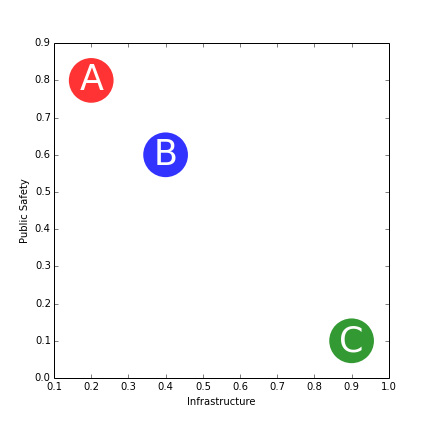
\includegraphics[width=0.7\textwidth]{figures/fisc_pos_concept}
\par\end{centering}

The figure demonstrates the concept of fiscal position in two dimensions.
Suppose Counties A, B, and C all had only two expenditure functions:
Infrastucture and Public Safety. We can relate their expenditure profiles
to one another by place the counties in space according to the proportion
of expenditures allocated to each function. In the figure, County
A is more similar to County B in expenditure preferences than County
C. This concept is scaleable to, if not depictable in, an aribitrary
number of dimensions.
\end{figure}


Counties that are ``close'' to each other in the expenditure space
have similar proportional distributions of expenditure. We will capture
county types as ``natural'' groupings of counties in this$n$-dimensional
space. In this framework, deflection of a given county from the group's
preferences will be identified by an increase in the distance between
the county's fiscal position and the central tendency in the group's
set of fiscal positions. To perform this task, two questions must
be answered:
\begin{enumerate}
\item How is the space defined?
\item How are clusters identified?
\end{enumerate}

\subsubsection{Defining Fiscal Space\label{sub:Defining-Fiscal-Space}}

To define the space in which fiscal positions were mapped, there were
actually two parallel tracks taken in the analysis. One track proceeded
as described above, in the $n$-dimensional space defined by the full
number of expenditure functions compared. While this approach facilitates
interpretation of any single dimension, the high number of dimensions
is 1) difficult to contemplate all at once, 2) impossible to visualize,
and 3) vulnerable to sparsity in broad swaths of the expenditure space.\footnote{Recall that estimation generally attempts to get at some form of local
averaging. To be efficient, that is, to minimize the variance in the
estimate, it requires that a number of observations are close to the
location being evaluated. There are only 64 counties evaluated in
any given year. If they all varied in the dependent value and in only
one independent dimension, we would likely be able to estimate with
a high degree of precision. As soon as a second independent dimension
is added, however, the area in which observations may reside increases
dramatically. It becomes much less likely that observations are close
enough together to provide the estimating precision experienced with
only one independent dimension. This potential observation space increases
yet again with a third dimension, and further still with a fourth.
In general, each new dimension one adds to the model requires a substantial
increase in the number of observations needed to maintain the same
estimating precision.}

One approach that mitigates these concerns is the dimension-reduction
technique known as principal component analysis (PCA). This method
enables one to leverage linear combinations of the original dimension
set. It is used here to place counties in three dimensional space,
albeit at a cost of a reduction in interpretability for each of the
resulting dimensions. In other words, moving along a given dimension
in the principal component space (e.g. $x_1=5d_1 + 3d_2 + 4d_3$ where
$d_*$ could represent public safety) is much more difficult to characterize
than moving along a given dimension in the original $n$-dimensional
space (e.g. $x_1=d_1$). To the extent that our main concern is the
magnitude of the distance between a county and its start group, we
can still pull useful information out of this approach, even if it
is difficult to explain precisely how a county is different. In any
event, since one track's weakeness is the other's strength, the parallel
tracks are complementary. If consistent results are seen across both,
it adds strength to the findings. Henceforth, the $n$-dimensional
track will be referred to as Track 1, while the PCA track will be
referred to as Track 2.

To complicate things just a little further, Track 1 also employs a
limited dimensionality reduction protocol that will be known as Track
1a. The protocol in Track 1a first groups the original 16 expenditure
functions into eight subgroups (Table \ref{tab:Subgroups-for-Track-1a}).

\begin{table}


\caption{Subgroups for Track 1a\label{tab:Subgroups-for-Track-1a}}


\vspace{10bp}


\centering{}%
\begin{tabular}{l|c}
\textbf{Subgroup} & \textbf{Constituent Functions}\tabularnewline
\hline 
\hline 
\emph{General Government} & General Government\tabularnewline
\emph{Judicial} & Judicial\tabularnewline
\emph{Public Safety} & Police, Fire, Other Public Safety\tabularnewline
\emph{Public Works} & Street, Trash, Other Public Works\tabularnewline
\emph{Health and Social Services} & Health, Social Services\tabularnewline
\emph{Captial Improvements and Debt Service} & Capital Outlays, Principal Service, Interest Service\tabularnewline
\emph{Intergovernmental} & Outgoing Transfers\tabularnewline
\emph{Miscellaneous} & Recreation, Miscellaneous\tabularnewline
\end{tabular}
\end{table}


The second step of this protocol leverages the fact that our primary
concern is the impact of COTEL intensity on fiscal behavior. Consequently,
only those dimensions that are actually affected by TEL imposition
are retained. In other words, inclusion in the final model is determined
by whether or not the expenditure category has a meaningful relationship
with COTEL intensity, as indicated by a series of bivariate regressions.
The procedure for selection of subgroups is discussed in Paragraph
\ref{par:Selection-of-Expenditure-Subgroups}.


\paragraph{Selection of Expenditure Subgroups\label{par:Selection-of-Expenditure-Subgroups}}

To select from the subgroups identified in Table \ref{tab:Subgroups-for-Track-1a},
there are two properties that must be identified:
\begin{enumerate}
\item The extent of variation in each subgroup's proportional contribution
to the entire expenditure portfolio.
\item The amount of each subgroup's variation\emph{ that can be associated
with variance in COTEL intensity.}
\end{enumerate}
The first conditions the findings of the second. Though in reality
the impact of COTEL intensity has been evaluated for all subgroups,
those subgroups that vary the least are not as desirable. The variation
in subgroup contribution can be seen in Figure \ref{fig:Distribution-of-Subgroup-Proportions}.

\begin{figure}


\caption[Expenditure Subgroup Proportions]{Distribution of Subgroup Proportional Contribution to Total Expenditures\label{fig:Distribution-of-Subgroup-Proportions}}


\centering{}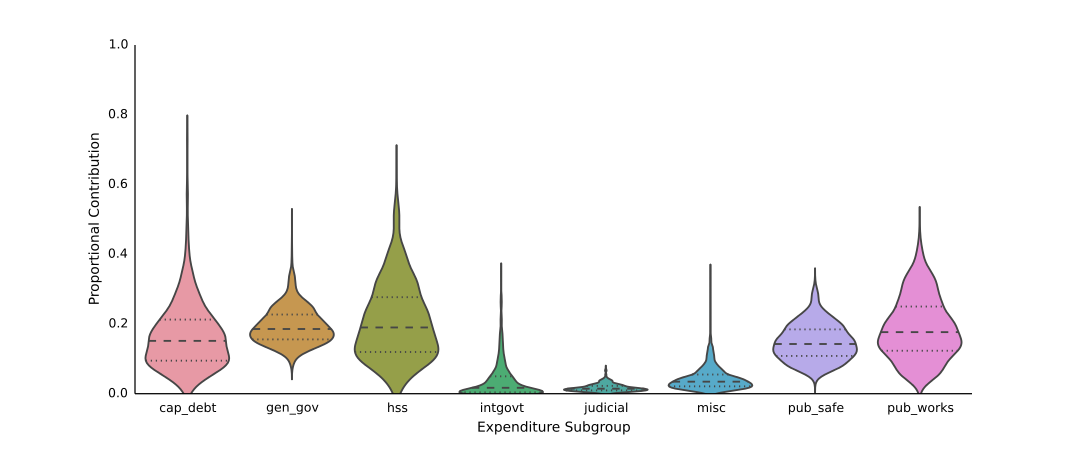
\includegraphics[width=1\textwidth]{figures/exp_subgroup_dist}
\end{figure}


To associate movement in each subgroup as a function of COTEL intensity,
a series of models have been run on two different COTEL intensity
concepts:
\begin{description}
\item [{Intensity~flow}] is the gap between allowable revenue yield under
TABOR/SLPTR and that which would be possible based upon economic conditions
within a county.
\item [{Intensity~stock}] is the cumulative impact of intensity flow.
\end{description}
For each intensity concept, two sets of models tested association
with transformed versions of the subgroup proportions. These transforms,
demeaning and standardization, were employed to capture only within
county variation due to COTEL intensity. As can be seen in Figure
\ref{fig:Intensity-vs-Exp-Subgroup}, both sets of models yielded
similar results.

\begin{figure}


\caption[COTEL Impact on Expenditure Subgroups]{Impact of COTEL Intensity on Individual Expenditure Subgroups\label{fig:Intensity-vs-Exp-Subgroup}}


\centering{}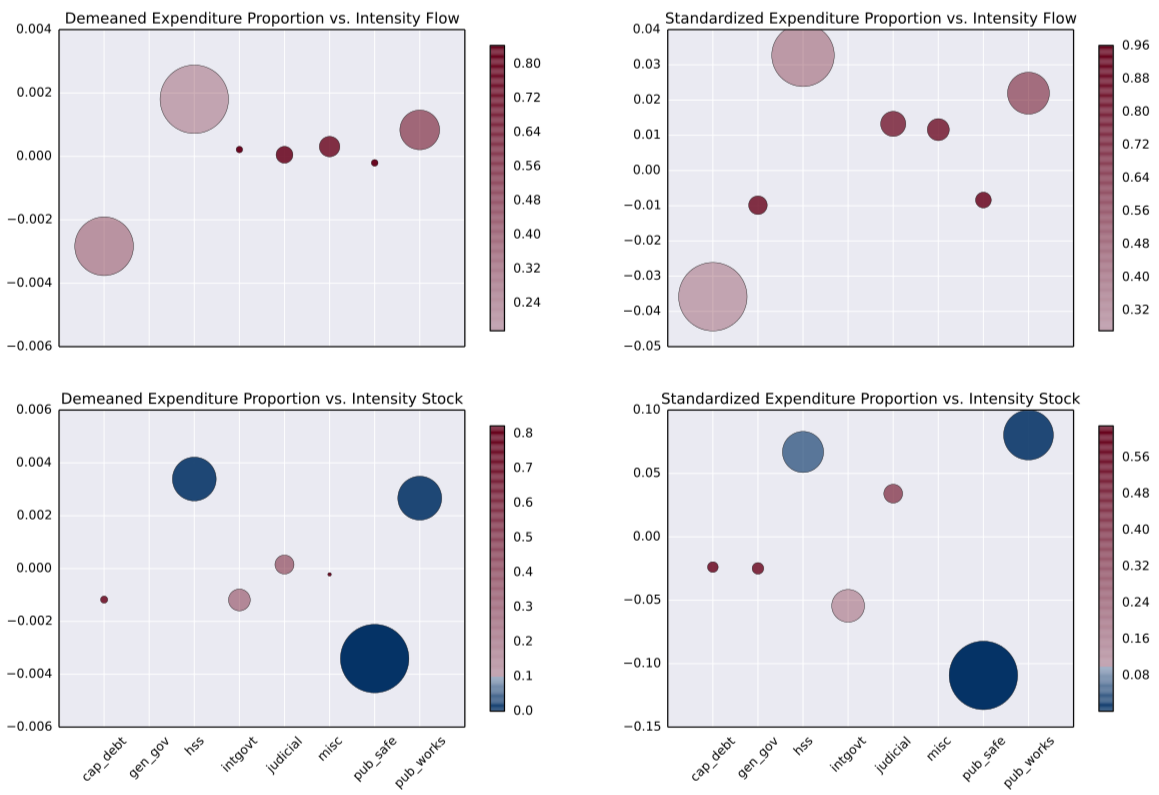
\includegraphics[width=1\textwidth]{figures/COTEL_intensity_vs_exp_subgroups}
\end{figure}


The coefficient estimates are captured as the y-axis position, the
fit ($R^2$) by the size of the bubble, and the statistical significance
by the color. As can be seen, intensity flow had negligible impacts
on the expenditure subgroups. The intensity stock models identified
three subgroups of interest: health and social services, public safety,
and public works.

It is interesting to note that the two dimension reduction procedures
(PCA and regression selection) highlight different aspects of the
fiscal portfolio. The variation in public works-related expenditures
is a common theme, as is health and social services. However, there
is some disagreement in the public safety area. This underscores the
need for three flights of models using the distances calculated via
Track 1, Track 1a, and Track 2.


\subsubsection{Identifying County Expenditure Types}

A central pillar of this analysis involves the capacity to assign
types to individual counties. Which rule should be used to group counties
when no a priori classification information exists? What is required
is a classification scheme that is emergent, conditional on the data.
The approach employed here is\emph{ $k$-means clustering}. The technique,
implemented via the expression in Algorithm \ref{alg:k-Means-Clustering},
minimizes the total distance between members of the same cluster (within-group
variance).

\begin{algorithm}


\caption{$k$-Means Clustering\label{alg:k-Means-Clustering}}


\vspace{10bp}


\begin{centering}
$$\mathrm{argmin}_S\sum_{i=1}^k\sum_{x_j\in S_i}\| x_j-\mu_i\|^2$$
\par\end{centering}

\vspace{10bp}


The expression minimizes the sum of all distances between each point,
$x_j$, and its associated centroid, $\mu_i$, within each cluster,
$S_i$. There are $k$ clusters; $k$ is given as a parametric input.
The expression is referred to as the minimum sum of squared residuals
(SSM). Insofar as this approach defines groups without pre-existing
classification attributes, it is considered a member of the\emph{
unsupervised learning} class of estimators.
\end{algorithm}


The definition of position is of central importance, and it varies
with context. In the current case, each point ($x_j$) represents
the fiscal position of a county in one of the fiscal spaces defined
in Subsection \ref{sub:Defining-Fiscal-Space}. In a well behaved
case, in which the clusters are reasonably well defined, the clustering
algorithm returns groups as seen in Figure \ref{fig:Well-Behaved-Clusters}.
Our fiscal position data is not nearly as well behaved, but $k$-means
clustering still provides a framework for cluster selection. 

\begin{figure}


\caption{Well Behaved Clusters\label{fig:Well-Behaved-Clusters}}


\begin{centering}
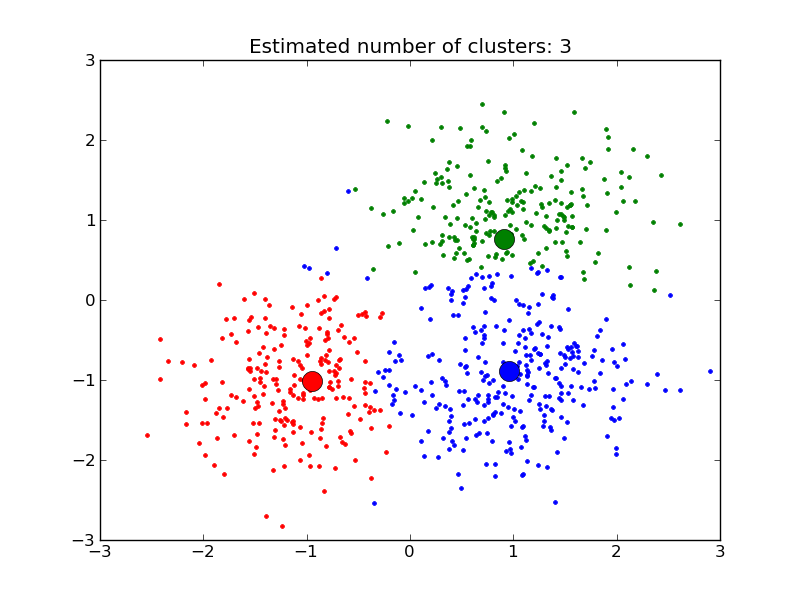
\includegraphics[width=1\textwidth]{figures/kmeans_ideal}
\par\end{centering}

Group membership is defined here by color. The centroids of each group,
or cluster, are represented by the large markers of each group's color.
Note that the centroid markers\emph{ do not represent observations.}
Rather, they are calculated measures of within-cluster central tendency.
The image is attributed to the documentation of the \href{http://scikit-learn.org/stable/}{scikit-learn library}.
\end{figure}


From an operational perspective, the clustering analysis was performed
based upon fiscal positions in the PCA space. The reasons for this
are two-fold. First, the dimension reduction techniques (PCA and regression
filtering) allow us to distill down to three dimensions, which facilitates
visualization. As it turns out, visualization is a very useful way
of checking the face validity of the algorithm's output. Second, PCA
is preferable relative to the regression filtering approach because
it retains nearly all of the information in the original set. This
is because the new dimensions are just complex combinations of the
old dimensions, and the first three components explain 88.5\% of the
variation in the data (Figure \ref{fig:Variation-in-Exp-PCA}).

\begin{figure}


\caption[Principal Components of Expenditure]{Variation in Principal Components of the Expenditure Portfolio\label{fig:Variation-in-Exp-PCA}}


\centering{}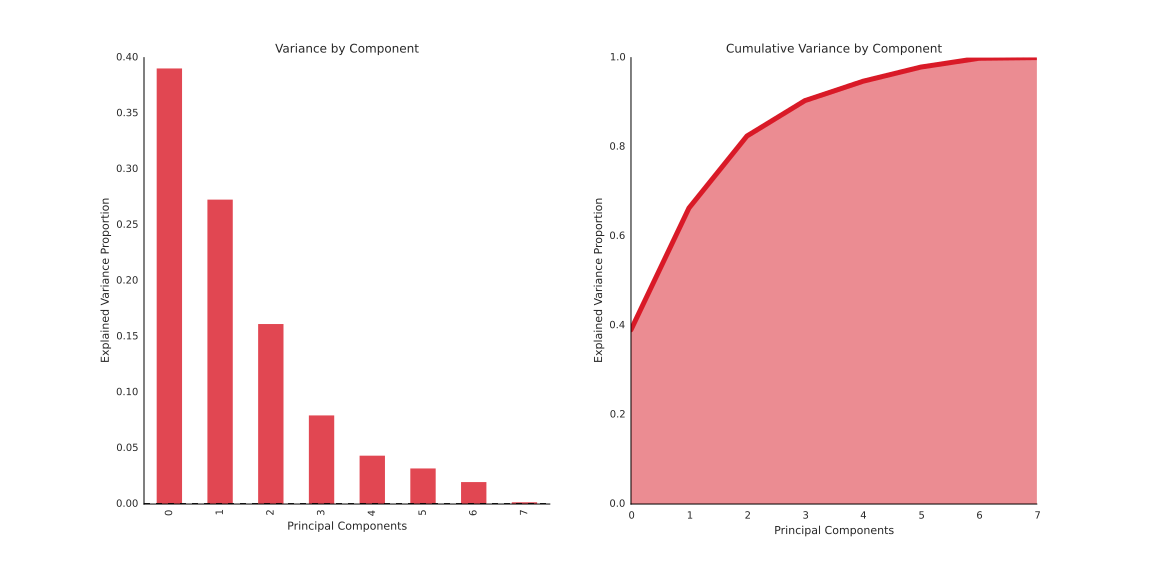
\includegraphics[width=1\textwidth]{figures/exp_pca}
\end{figure}


Recall that the major drawback of the PCA approach is the interpretation
of movement along one of the compound dimensions that remain. However,
if all that matters for this particular operation is the proximity
of fiscal positions across counties, interpretation of the linear
combinations of underlying dimensions is not the principal concern.
Consequently, the space defined by PCA is unambiguously superior to
the space defined by regression filtering for the purpose of identifying
clusters of county fiscal preferences.


\paragraph{Choosing the Appropriate Number of Clusters $k$}

It is important to reiterate that the use of $k$-means clustering
requires the number of groups, $k$, to be a parametric input. Therefore,
there is a certain amount of subjectivity involved, because the optimal
value of $k$ is unknown.\footnote{If, for example, one were to choose $k$ such that the aggregate distance
between points within each cluster was minimized, one would find that
$k\to n$ where $n$ is the number of observations. In other words,
each cluster would shrink to contain only a single observation.} This subjectivity is particularly prominent when group boundaries
are not clean. The fiscal positions of Colorado counties in 1975 are
displayed in Figure \ref{fig:Fiscal-Positions-1975}.

\begin{figure}


\caption[Fiscal Positions - 1975]{Fiscal Positions of Counties in Colorado in 1975\label{fig:Fiscal-Positions-1975}}


\begin{centering}
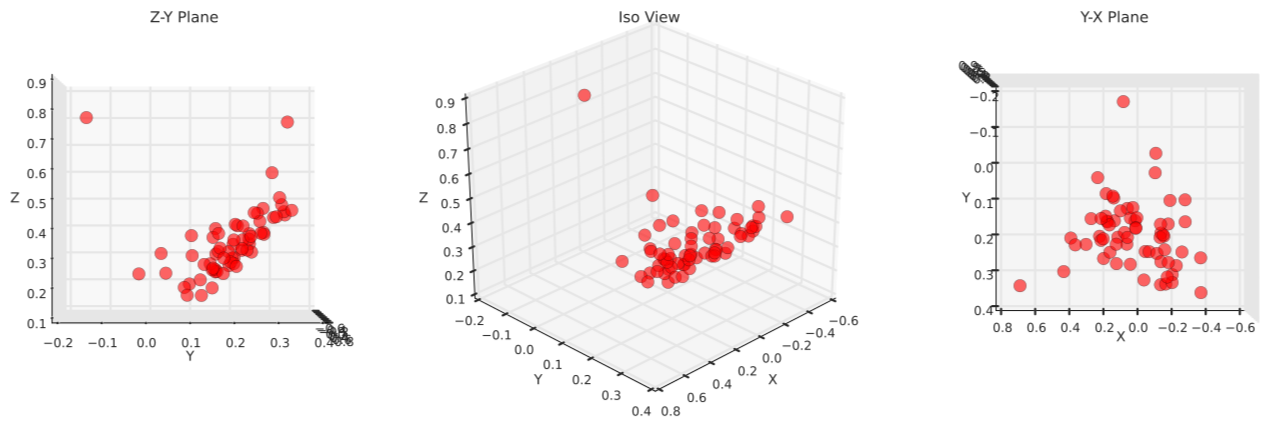
\includegraphics[width=1\textwidth]{figures/fisc_pos1975}
\par\end{centering}

Note that the fiscal positions are not as well-behaved as the ideal
case above.
\end{figure}


To lessen the influence of the subjectivity in selecting the number
of groups, this analysis tested a range of values for $k$. This allows
one to evaluate the impact on SSM of additional clusters. That being
said, variance in group count, $k$, is a useful but insufficient
means for identifying the correct clustering profile. On the one hand,
SSM is\emph{always} a non-increasing function of the number of groups
$k$. On the other hand, it is simply desirable to minimize the number
of required groups because evaluating the dynamics of a group is less
than useful if it has only a few members. To mitigate the tension
between these two desirable properties and determine the number of
clusters to be used for econometric analysis, three tests augmented
visual inspection of clustering:
\begin{enumerate}
\item The first method evaluates the marginal contribution to\emph{ between-cluster
variation} of each cluster. The technique seeks to understand movement
in the ratio of between-cluster variation to total variation in the
sample. The desirable number of groups is then the value,$k$, at
which the increase in the ratio increase over the interval $[k-1,k]$
is significantly higher than the ratio increase over the interval
$[k,k+1]$.
\item The second method evaluates the marginal contribution to\emph{ within-cluster
variation} of each cluster. As previously indicated, this function
decreases with increases in the number of groups $k$. When intersected
with the first method, the result is a balancing of separation across
clusters and similarity within clusters.
\item The third method is a popular selection mechanism known as the ``silhouette
score''. In this case, the number of clusters is identified by maximizing
the aggregate distances of observations in cluster $i$ from the centroid
of all groups $j$ (where $i\neq j$),\emph{ relative to the points'
distance from their own centroid in group} $i$.
\end{enumerate}
The test ensemble suggested that the optimal cluster count, $k$,
lies on the interval $[5,8]$. Within these bounds, selection proceeded
via visual inspection of the clustering outcomes at each value of
$k$. Ultimately, five clusters were found to provide the cleanest
separation of groups.

\begin{figure}


\caption[Fiscal Clusters$k=5$]{Fiscal Clusters$k=5$\label{fig:Fiscal-Clusters-k5}}


\begin{centering}
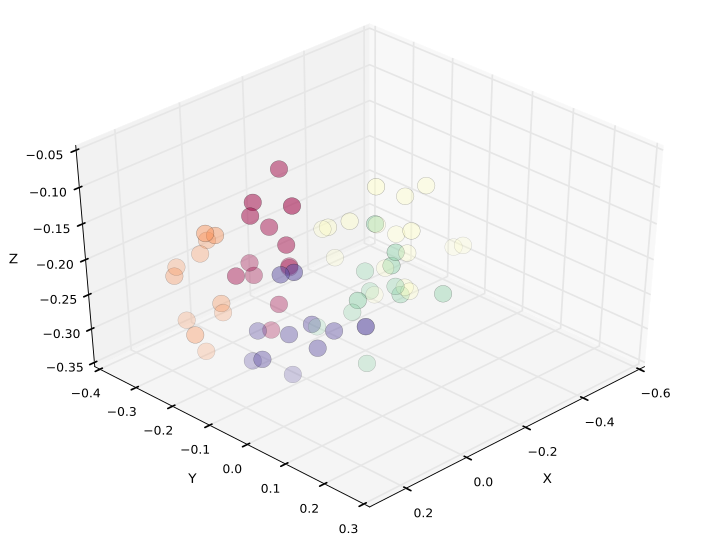
\includegraphics[width=1\textwidth]{figures/fisc_pos1975_k5}
\par\end{centering}

Visual identification of clusters in 3-dimensional space is difficult
with static views. The selection process leveraged animated rotation
of several plots to facilitate cluster count choice.
\end{figure}



\paragraph{Do Distances to Cluster Centroids Vary?}

Just as it was necessary to establish variation in fiscal clustering
in Chapter \ref{chap:RevYieldCapacity}, the existence of meaningful
variation in the distances between individual counties and their cluster's
centroid must be established here. Without said variation, we would
be unable to associate variation in COTEL intensity with variation
in the distance of each county from its centroid.\footnote{Recall that distances to cluster centroids are how we measure wedges
between an individual county and the prevalent expenditure preference
schedule of similar counties.} In Figure \ref{fig:Within-Cluster-Variation} we see violinplots
of cluster distances within each group, as well as the coefficient
of variation for county distances for each group.

\begin{figure}


\caption{Within-Cluster Variation\label{fig:Within-Cluster-Variation}}


\centering{}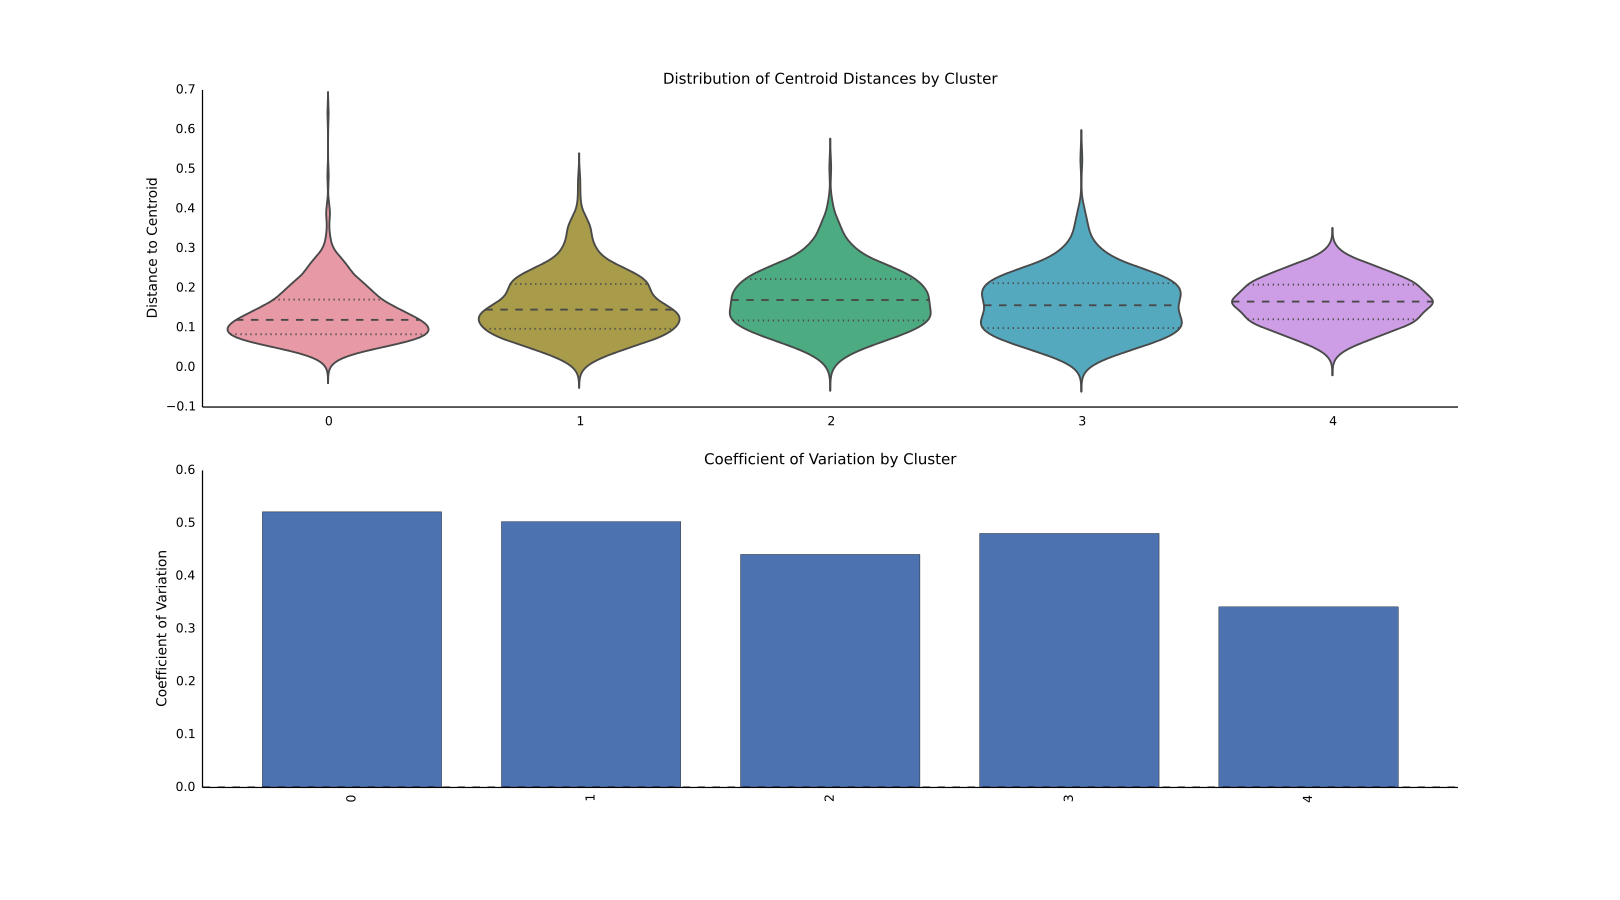
\includegraphics[width=1\textwidth]{figures/clust_dist_variance}
\end{figure}


It is interesting to note differing variation profiles within each
group, which supports the idea that they are rightfully distinct in
this analysis. As can be seen in Figure \ref{fig:Within-Cluster-Variation-by-Year},
the overall distance to cluster increases modestly over time. In other
words, there is some evidence of the variety in expenditure profiles
across all counties increasing over time.

\begin{figure}


\caption{Within-Cluster Variation by Year\label{fig:Within-Cluster-Variation-by-Year}}


\centering{}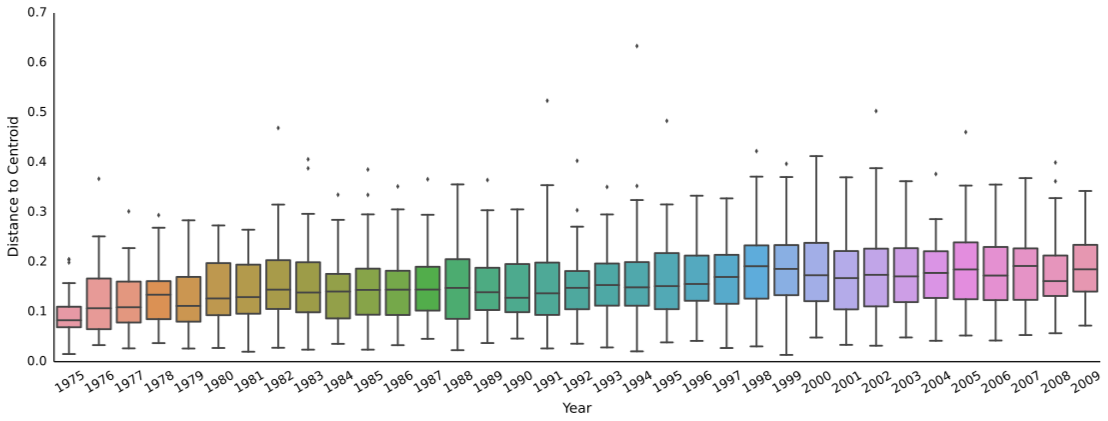
\includegraphics[width=1\textwidth]{figures/clust_dist_variance_yr}
\end{figure}



\paragraph{Caveat Emptor}

The last view considered prior to modeling is the\emph{ within-county}
variation in distance to the associated centroid. In Figure\ref{fig:cty-clust-dist-var},
the distribution of cluster distances across years is displayed by
county. On the positive side, it reinforces the idea that counties
within a cluster can behave quite differently over time. The analysis
seeks to leverage this variation in behavior to understand the impact
of COTELs.

\begin{figure}


\caption{Within-County Variation of Distance to Cluster\label{fig:cty-clust-dist-var}}


\begin{centering}
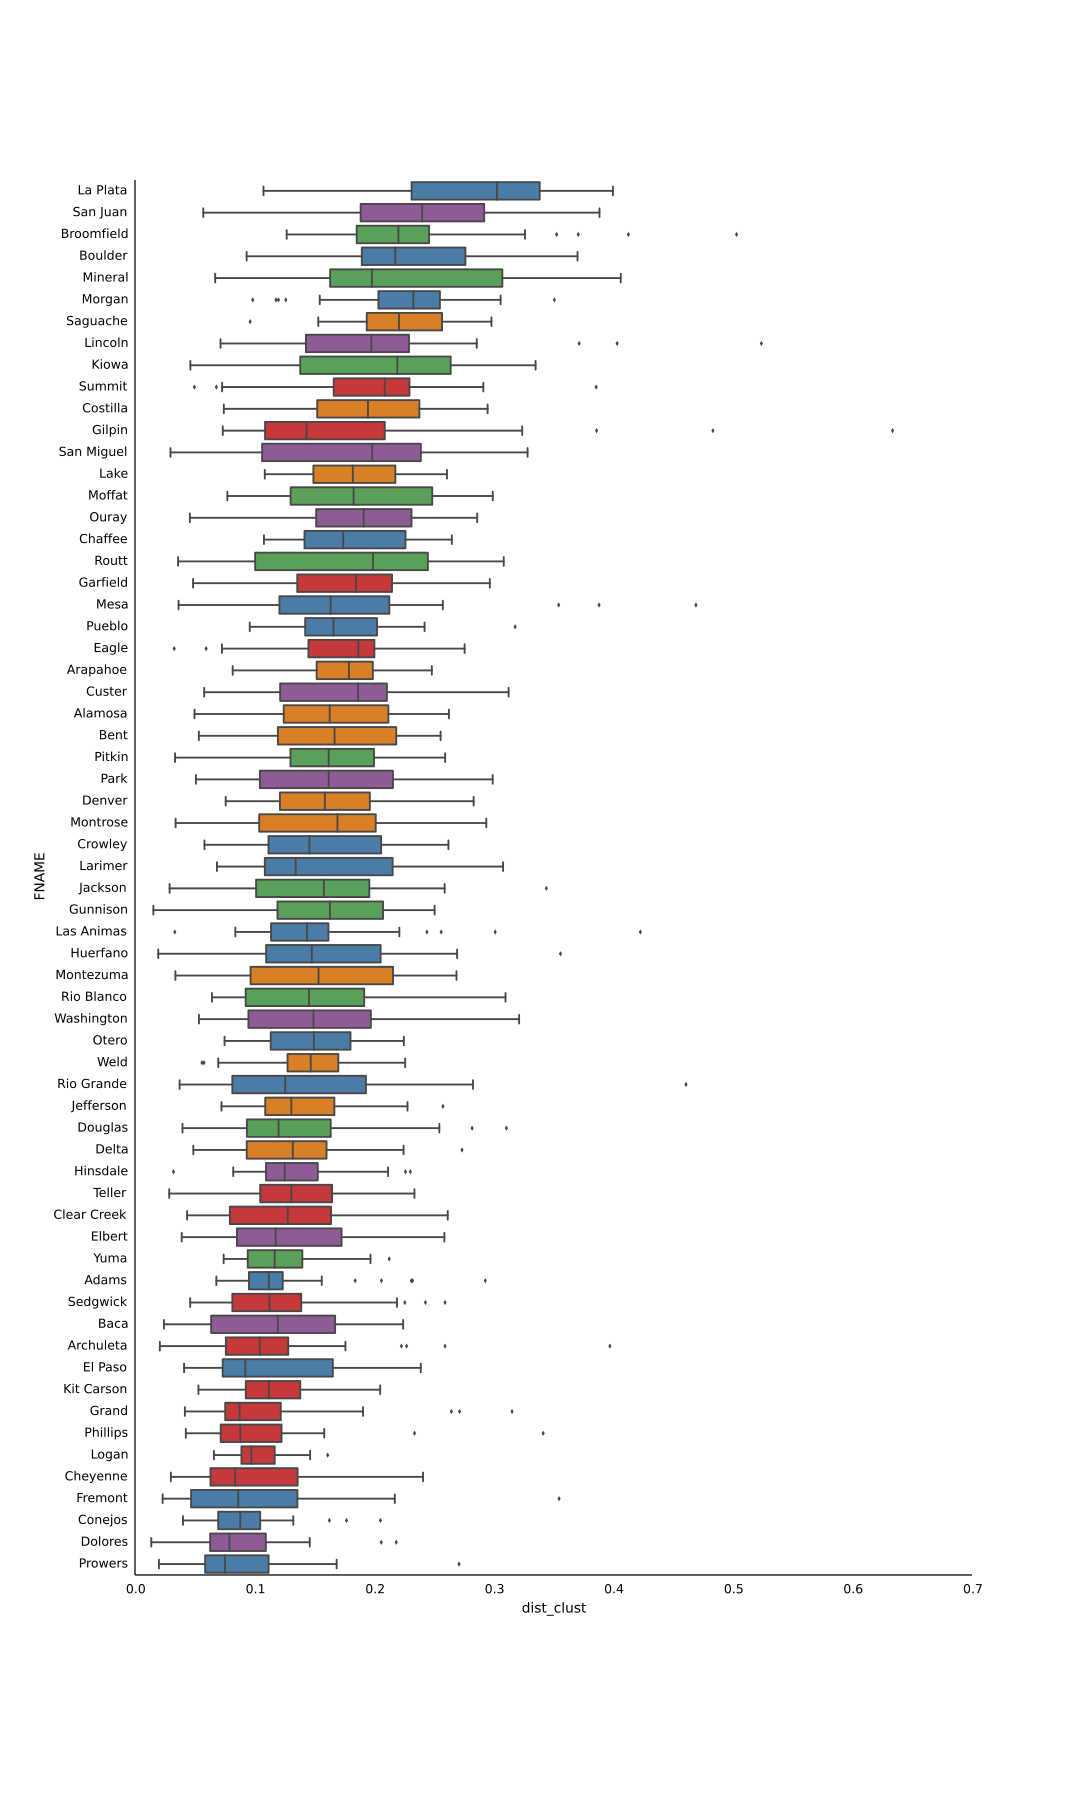
\includegraphics[width=0.8\textwidth]{figures/clustDist_var_cty}
\par\end{centering}

The counties are colored by type. Note that these distances are not
measured from the same location, but rather the location of the centroid
of each county's associated type.

\end{figure}


However, this view does some violence to the idea of constant covariance
in within-cluster expenditure preferences. First, while we seek to
identify within-cluster differences associated with COTELs, other
differences capture inherent disimilarity as well. Second, there is
an assumption that counties do not change types, but it is plausible
that the variation seen in Figure \ref{fig:cty-clust-dist-var} would
lead to different types at different times. Again, if this is due
to COTELs, this is a useful finding. If it is due to other factors,
it again highlights inherent disimilarity.

Thus, some weaknesses of the constant covariance approach certainly
exist, but as discussed in Subsection \ref{sub:Typification-Reasonable},
it is likely to be a less costly assumption than alternative assumptions
that can be made. In general,\emph{ there does not exist a unique
approach that may reveal the fundamental nature of the phenomenon
in isolation.} Hoover reflects usefully on the general selection of
an estimation approach:
\begin{quotation}
``{[}T{]}he thorough-going optimization implicit in new classicism
suggests that everything depends on everything else, not just in theory,
but in practice. {[}...{]} Thus, theory presents us with some a priori
(in the sense of not\emph{ currently} questioned) restrictions on
empirical investigation; while the empirical results help us generate
beliefs (or new theories) which are prior to further investigations.''\citep{Hoover1994}
\end{quotation}
In other words, we restrict the lens through which we view the observable
implications of some unseen phenomenon. While the lens may be defensible,
each choice suffers from the weakness of our a priori belief about
how said lens ought to be defined. No single view should be evaluated
as having incorporated the full complexity of the system under study.
Rather, we take simplified cuts at the data generating process, and
converge on ``reality'', with confidence increasing in the number
of supporting analytic outcomes.

Given the basic establishment of statistical identification, it is
important to consider the impact of the boundaries imposed by a given
method (e.g. constant covariance). The concern, from a utility standpoint,
is whether or not the boundaries are responsible for driving measurement
outcomes, as opposed to the underlying data generating process. Indeed,
it was with this liability in mind that the decision was made to leverage
data driven classification in the first place. $k$-means clustering
does take a single parameter, $k$, but it does not otherwise impose
any distributional assumptions.

In the end, the approach taken here must not be viewed as a substitute
for the views that would be revealed by other approaches, inclusive
of those considered in Subsection \ref{sub:Typification-Reasonable}.
Rather, this approach, unique to the best of the author's knowledge,
provides an important view of the underlying data that should be considered
in a comprehensive assessment.


\section{What is the Expected Impact of TELs?}

The frame for this analysis is the ``expenditure wedge''. Do constrained
jurisdictions deflect from their preferred expenditure bundles? It
is hypothesized that any such deflection would be in the direction
of providing a minimum bundle of services, and it is expected that
the minimum bundle reflects a fairly consistent set of needs for any
general purpose jurisdiction (Model \ref{mod:exp_impact}). Therefore,
paring down to the minimum bundle would limit the capacity of a given
jurisdiction to distinguish itself from other jurisdictions. It is
further expected that the impact of this convergence will be strongest
in low-income jurisdictions, where resources are already constrained.
The work of Mullins and Joyce\citep{Joyce_Mullins1991} has revealed
that binding TELs are associated with shifts of expenditure responsibility
to the state level, which also promotes uniformity in service delivery
(or at least in the resources allocated). This study evaluates what
counties in Colorado do with the remaining resources. What does their
expenditure profile look like when TELs have taken effect?

\begin{model}


\caption[COTELs and Expenditure Behavior]{What is the Nature of COTEL Impact on Expenditure Behavior?\label{mod:exp_impact}}


\vspace{10bp}

\begin{description}
\item [{Expenditure~Differentiation}] =\emph{f}(Resources to Cover the
Minimum Service Bundle, Excess Resources)
\end{description}
\vspace{5bp}


where

\vspace{5bp}

\begin{description}
\item [{Resources~to~Cover~the~Minimum~Service~Bundle}] =\emph{f}(Demographic
Factors, Geographic Environment)
\item [{Excess~Resources}] =\emph{f}(Revenue Base Dynamics, Institutional
Restrictions on Revenue)
\end{description}
\vspace{10bp}


In effect, the model in this study suggests that institutional restrictions
on revenue (e.g. tax and expenditure limitations) restrict the resources
available to cover services that would allow a given jurisdiction
to differentiate itself from others. In reality, this is a gross simplification.
There is no natural boundary between revenues used to cover basic
services and those used to cover the additional services preferred
by constituents. In general, this model suggests convergence in expenditure
behavior would stem from the imposition of COTELs.
\end{model}
If expenditure behavior shifts, a wedge is thrown between the realized
and preferred tax-expenditure bundle for a given county. For prospective
residents, the choice set is more limited, and the properties that
may have drawn them to a particular county are less of a factor. For
existing residents, an artificial difference has been created between
the initial, expected utility that factored into the decision to site
in the county and the realized utility after the expenditure shift
has occurred. In practice, this may or may not lead to a reshuffling
for those residents that can afford to move. Those that cannot simply
experience a loss in utility. Furthermore, if the choices in close
proximity lose some of their differentiation, the cost of relocating
to a more ``desirable'' county increases. In any event, understanding
the impact of loss in differentiation is important for a comprehensive
view of COTEL impact.


\section{Do TELs Shift Patterns of Expenditure?}

Our primary inquiry centers on whether or not the distance of a given
county from the average preference position of counties of that type
can be explained to some meaningful degree by the intensity of the
COTEL constraint acting on said county. In measuring this, it is important
to control for confounding economic processes that may impact cluster
distance. These economic processes may occur in both the current observation's
county, and the adjoining counties that may share bases of economic
activity. In other words, the model must account for both the primary
county, and the counties in the local neighborhood. Model \ref{mod:clust-dist-model}
captures this process in a general way.

\begin{model}


\caption[Determinants of Cluster Distance]{Modeling Determinants of Cluster Distance\label{mod:clust-dist-model}}


\vspace{10bp}


$$y_{it} =\underbrace{W y_{i_-,t}\Gamma_1}_{(1)} +\underbrace{\sum_{l=1}^L y_{i,t-l}\Gamma_2}_{(2)} +\underbrace{Z_{i,t}\beta}_{(3)} +\epsilon_{i,t}$$

where

$$Z_{i,t}\beta =\underbrace{W X_{i_-,t}\beta_1}_{\text{(3a)}} +\underbrace{X_{i,t}\beta_2}_{\text{(3b)}} +\underbrace{X_t\beta_3}_{\text{(3c)}}$$

\vspace{10bp}

\begin{description}
\item [{$y_{i,t}$}] is the dependent variable ($clust\_dist$), the distance
of county $i$ at time $t$ from the centroid of its cluster (a.k.a.
cluster distance). Note that $y_{i_-,t}$ denotes the cluster distance
of each county $j$ at time $t$ where $i\neq j$.
\item [{$W$}] is the weight matrix that defines the ``local neighborhood''.
\item [{$\Gamma$}] represents the coefficients of autoregressive terms.
$\Gamma_1$ is for the spatially autoregressive effect, while $\Gamma_2$
is for the temporally autoregressive effect.
\item [{$Z_{i,t}$}] is a vector of regressors that includes the primary
variables of interest, $intensity\_stock$ and $prop\_ratio$. These
include factors from the local neighborhood, county-specific factors,
and statewide factors.
\item [{$\epsilon_{i,t}$}] is the error term.
\end{description}
The model can be broken down into components, each of which are numbered
above. The top line equation captures spatial autoregression in cluster
distance (1), temporal autoregression in cluster distance (2), and
forces acting on the primary county at time $t$ (3). The second equation
unpacks term 3. It captures select properties of counties in the local
neighborhood (3a), county-specific properties (3b), and statewide
variables (3c). The breakdown of variables in term 3 are as follows:
\begin{description}
\item [{Term~3a}] includes total expenditures ($EXP\_TOTAL$), population
growth in the preceding year ($pop\_growth$), and the ratio of vacant
housing units to total housing units ($vac\_rate$).
\item [{Term~3b}] includes total expenditures ($EXP\_TOTAL$), population
growth in the preceding year ($pop\_growth$), intergovernmental revenue
per capita ($pcintgov$), total revenue per capita ($pcrev$), annual
payroll per capita ($pcap$), COTEL intensity ($intensity\_stock$),
and the Gallagher ratio ($prop\_ratio$). The term also includes an
interaction between COTEL intensity and total expenditures ($exp\_intensity$)
to capture variance in intensity impact along the fiscal resources
dimension.
\item [{Term~3c}] includes a single variable, gross state product in the
previous year ($gsp.L$).\end{description}
\end{model}


In practice, Model \ref{mod:clust-dist-model} is captured in two
separate model classes. The first is the spatially autoregressive,
cross-sectional model:

$$y_i = Wy_{i_-}\Gamma + Z\beta +\epsilon$$

The second is a conventional temporally autoregressive model; it is
generally known as an AR(1) model:

$$y_{i,t} = y_{i,t-1}\Gamma + Z_{i,t}\beta +\epsilon_{i,t}$$

This split is largely due to the relative lack of spatial panel estimators
at the time of analysis.


\subsection{Variable Properties}

As can be seen in Figure \ref{fig:Var-Variation-Full}, the model
terms have very different variation profiles. While cluster distance
($dist\_clust$) does vary, the normalized view offered by the coefficient
of variation indicates that cluster distance does not vary nearly
as much as the other variables included in the analysis.\footnote{Note that any of the variables names preceded by $SL\_$ indicate
spatial lag versions of the base variable. That is, the value captures
the weighted average of all values in the local neighborhood as defined
by weight matrix $W$, except for the primary county $i$.}

\begin{figure}
\begin{centering}
\caption[Full Expenditure Portfolio Variables]{Variation in Model Variables - Full Expenditure Portfolio Distance\label{fig:Var-Variation-Full}}
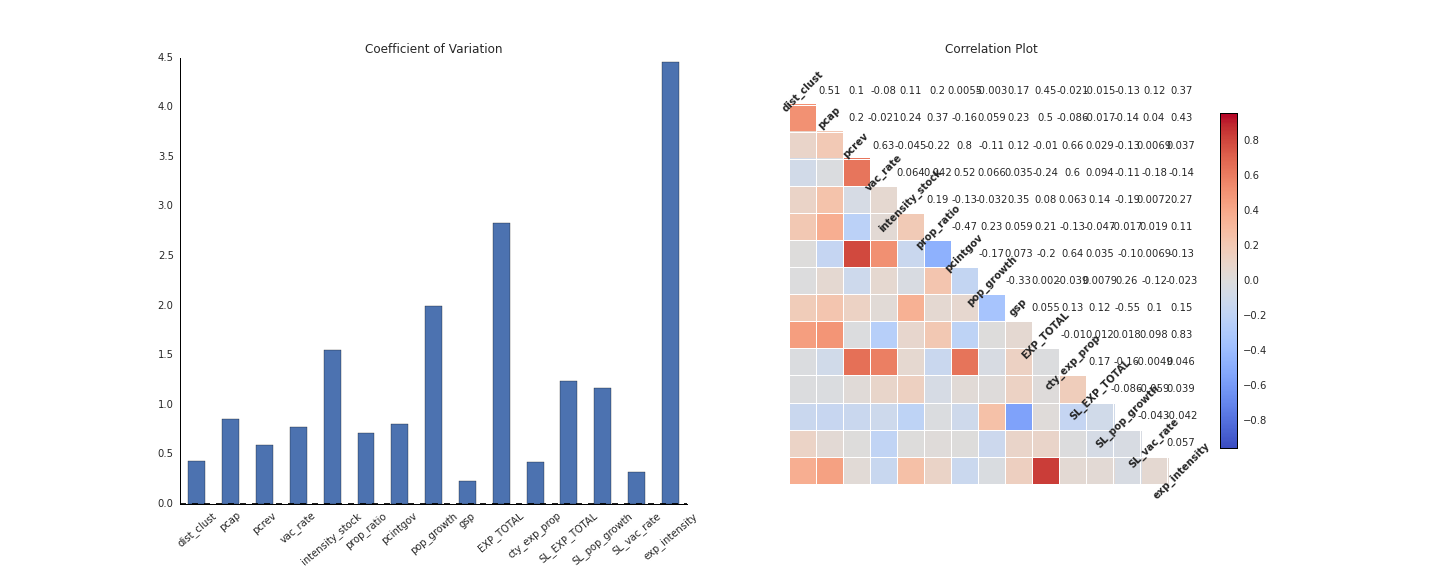
\includegraphics[width=1\textwidth]{figures/ExpDiv_varCorr}
\par\end{centering}

Note that COTEL intensity ($intensity\_stock$) is significantly correlated
only with the Gallagher ratio ($prop\_ratio$) and economic capacity
(as measured by annual payroll per capita;$pcap$).
\end{figure}


Our measure of similarity, or disimilarity as the case may be, is
$clust\_dist$. It proves to be useful, but it would be more so if
it varied over a greater range. Marginal impacts of regressors are
easier to identify when they are associated with larger absolute spans
in the range of dependent values. If a given dependent variable takes
one of only two values, the contributions of each regressor is more
difficult to distinguish relative to the case in which a dependent
variable\emph{ with the same support} (that is, the same range of
feasible values) takes any one of 100 values.

It would be interesting to know if the correlation dynamics shift
based upon the definition of cluster distance (Figure \ref{fig:Var-Variation-Alt-Dist}).
Recall that while all three distances are $\ell^2$ norms (a.k.a.
Euclidean distance), the dimensionality of the space in which these
distances are calculated varies in number and concept. For example,
the full expenditure portfolio set has 16 dimensions, one for each
expenditure concept. In the PCA set, there are three dimensions, and
each is a linear combination of some subset of the original 16.

\begin{figure}


\caption[Alternative Distance Variables]{Variation in Model Variables - Alternative Distance Measures\label{fig:Var-Variation-Alt-Dist}}


\begin{centering}
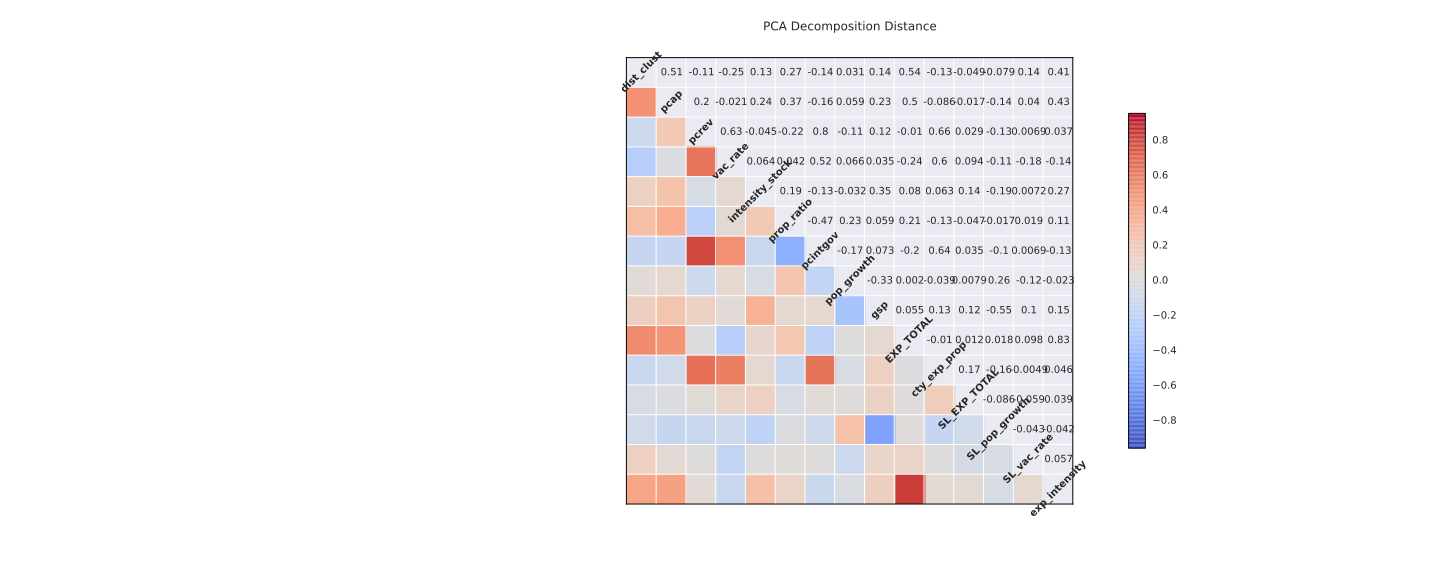
\includegraphics[width=0.4\textwidth]{figures/ExpDiv_varCorr_PCA}\hspace{2bp}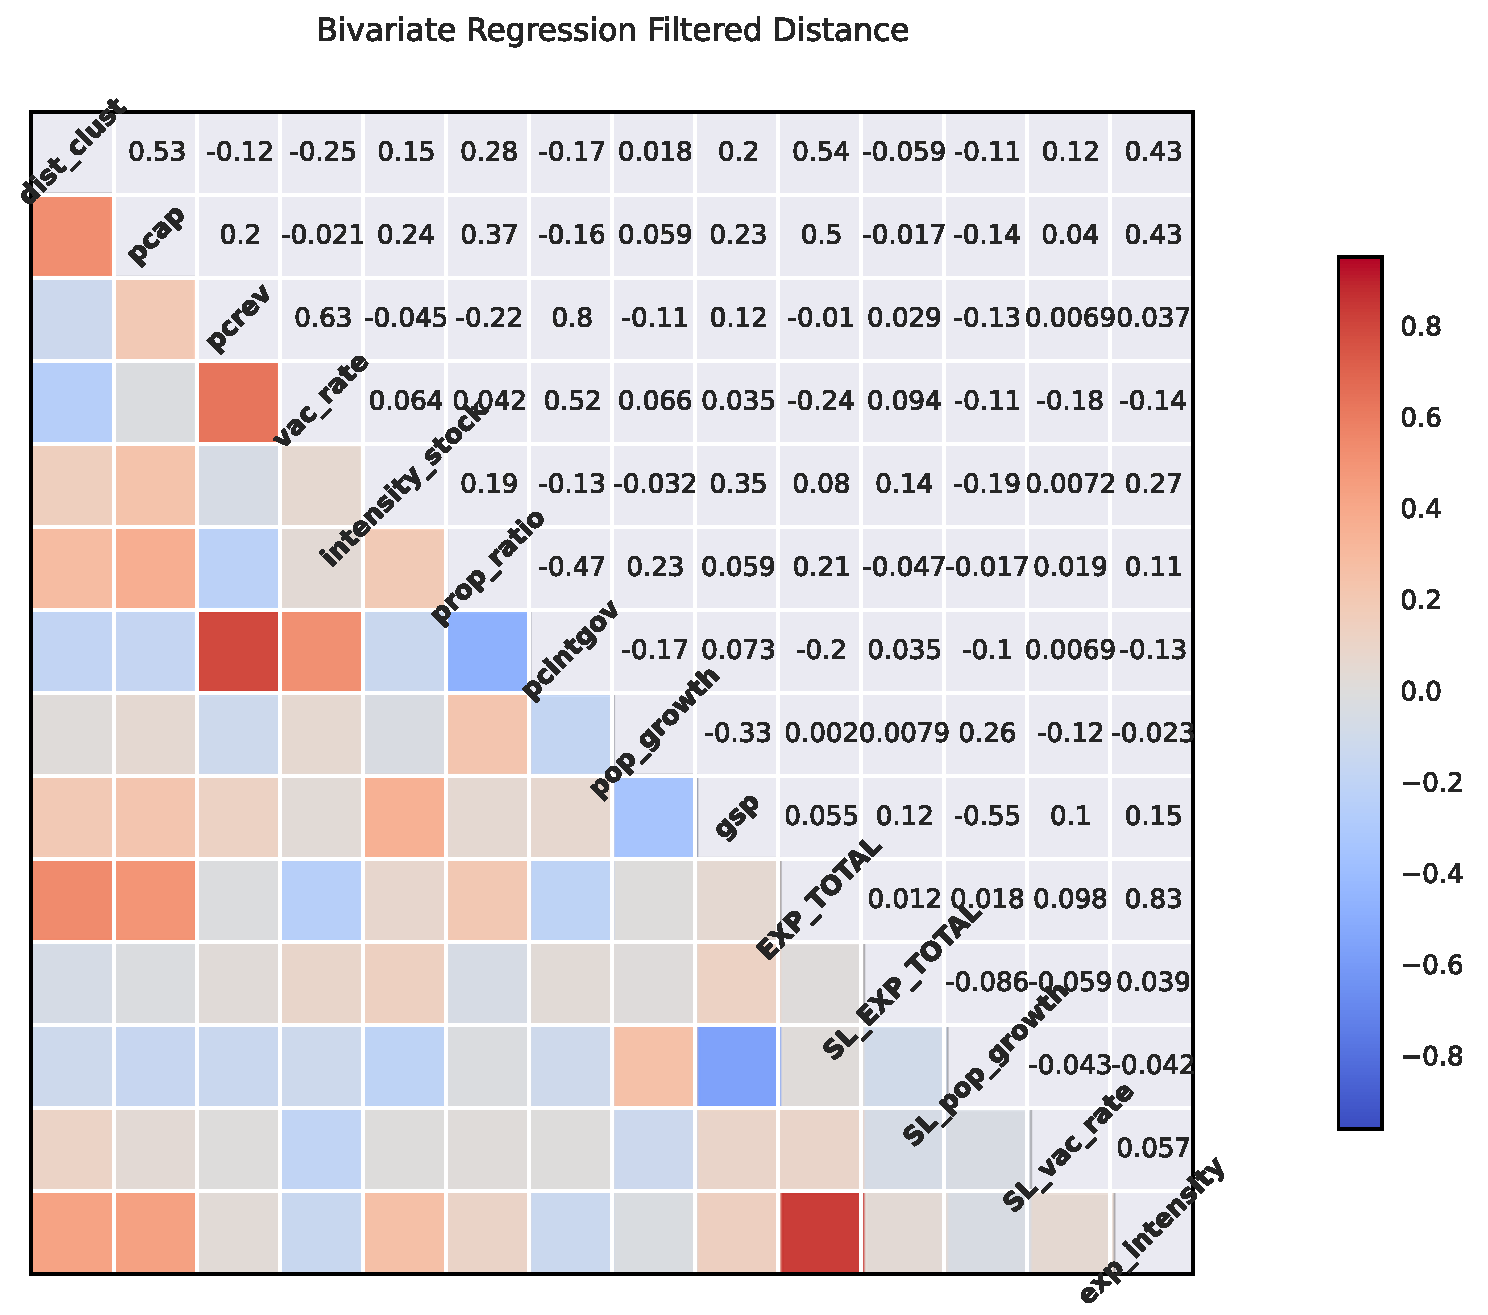
\includegraphics[width=0.4\textwidth]{figures/ExpDiv_varCorr_bivFilt}
\par\end{centering}

The significance of assosciation between cluster distance ($dist\_clust$)
and all other variables changes dramatically when distance is measured
in the PCA space. With respect to the regression filtered space, the
relationship between cluster distance and COTEL intensity ($intensity\_stock$)
is quite similar to full portfolio case. Furthermore, the relationship
between cluster distance and the Gallagher ratio ($prop\_ratio$)
is virtually identical. This suggests that the three dimensions that
remain were driving association in the full portfolio case anyway,
so paring down to them did not have as dramatic an effect as the switch
to the PCA case.
\end{figure}


While the statistical significance of association between cluster
distance and the COTEL variables does not meaningfully change, the
magnitude of association dropped in both cases. Moreover, the PCA
distance has fairly low association magnitudes with nearly all variables.
This suggests a substantially different variation profile for PCA
distance. One way to get a sense of how distance behavior varies across
the three frames is to observe the distribution of distance values
by county and basis for distance calculation.

\begin{figure}


\caption[Cluster Distance by Calculation Method]{Cluster Distance by Calculation Method by County\label{fig:clust-dist-by-method}}


\includegraphics[width=1\textwidth]{figures/ExpDiv_ctyVar_distCalc}

The space in which cluster distance was measured is indicated by color.
The\textcolor{red}{{} red boxplots indicate the distance was calculated
across the entire expenditure portfolio}. The\textcolor{blue}{{} bivariate
regression filtering space is show in blue}, and the\textcolor{green}{{}
PCA is shown in green}.
\end{figure}


The boxplot in Figure \ref{fig:clust-dist-by-method} is certainly
a busy visual display of variation in cluster distances. The takeway,
however, is not a precise estimate of variation. Rather, this chart
shows that the distribution of values differs markedly by calculation
method. To the extent that these distributions neither perfectly overlap
nor exhibit fixed relationships observed in all counties, it can be
inferred that the results of this analysis may be sensitive to calculation
methods. That being said, consistent findings from these models in
spite of this variation would be strong evidence in support of a real
relationship existing in the underlying data generating process (see
Subsection \ref{sub:Econometrics-as-Observation}).

\clearpage


\subsection{Cross-Sectional Models\label{sub:ExpDiv-Cross-Sectional-Models}}

Model \ref{mod:clust-dist-model} presents a view of the world that
represents the a priori belief of the author with respect to cross-sectional
action in county fiscal behavior. Given that county groups are not
defined spatially, and thus members are often not close to each other,
it seems quite plausible that the factors that may lead a county to
part ways with group behavior are spatial factors which would not
be shared across all members of the group. Thus, it is expected that
spatial dependency, either through lags or errors, would need to be
integrated into the analysis. The abstract and operational versions
of this view are provided in Model \ref{mod:Cross-Sectional-Estimation-of-Exp-Diverg}.

\begin{model}


\caption[SLM - Expenditure Divergence]{Cross-Sectional Estimation of Expenditure Divergence\label{mod:Cross-Sectional-Estimation-of-Exp-Diverg}}


\vspace{10bp}


$$y_i =\underbrace{W y_{i_-}\Gamma}_{(1)} +\underbrace{Z\beta}_{(3)} +\epsilon$$

where

$$Z\beta =\underbrace{WX_{i_-}\beta_1}_{(3a)} +\underbrace{X_i\beta_2}_{(3b)}$$

\vspace{10bp}


In terms of the variables, the model is as follows:

$$dist\_clust_i =\underbrace{W\times (dist\_clust\hspace{3bp}\forall\hspace{3bp} j)}_{(1)} +$$

$$\underbrace{SL\_EXP\_TOTAL + SL\_pop\_growth + SL\_vac\_rate}_{(3a)} +$$

$$\underbrace{EXP\_TOTAL + pop\_growth + pcintgov + pcrev + pcap + }_{(3b)}$$

$$\underbrace{prop\_ratio + intensity\_stock + EXP\_TOTAL*intensity\_stock}_{(3b)}$$

where $i\neq j\hspace{3bp}\forall\hspace{3bp} i\in S$ and the $SL\_$
prefix indicates the spatial lag (the average value in the local neighborhood,
$S$).
\end{model}


To check the face validity of the spatial assumption, one can use
a global version of the Moran's I calculation defined in Algorithm
\ref{alg:Local-Moran's-I}. While the global calculation does not
permit the identification of hot spots, or clusters, within the state,
it does have the advantage of providing a single statistic that captures
the existence of clustering somewhere within the state. As such, we
can evaluate clustering over time more easily. Figure \ref{fig:Moran's-I-dist_clust-yr}
displays clustering activity in Colorado over time, faceted by six
distance dimensions. The first three (Full Portfolio, Regression Filtered,
and Principal Components) correspond with the distance measures calculated
in the spaces defined in Subsection \ref{sub:Defining-Fiscal-Space}.
The second three are transformations of the first three. They are
change measures that capture the difference in cluster differences
between the current year (year $t$) and the next year (year $t+1$).

\begin{figure}


\caption{Moran's I - Cluster Distance by Year\label{fig:Moran's-I-dist_clust-yr}}


\begin{centering}
\includegraphics[width=1\textwidth]{figures/ExpDiv_CD_Moran}
\par\end{centering}

The figure depicts the value of Moran's I for each distance measure
by year. Higher values indicate clustering of similar values while
lower values indicate clustering of disimilar values. A value of zero
should be interpreted as the absence of clustering. In other words,
the distribution of cluster distances is relatively random across
counties. The color of each observation captures the statistical clarity
of the clustering behavior (i.e. $p$-value). 
\end{figure}


There are three properties of the Figure \ref{fig:Moran's-I-dist_clust-yr}
that are of particular interest. First, the identification of spatial
clustering varies dramatically across different measures of distance.
Second, leading change measures are generally less spatially coherent
than current year absolute measures. Third, the current year full
portfolio distance measure is the only one that seems to exhibit spatial
clustering over most of the period, \emph{and that clustering intensity
declines over time}. In short, while it seems as though regional dynamics
could play an outsized role in causing counties to stray from the
behavior of their initial types, the data seem to suggest that this
expectation is overstated.

\begin{figure}


\caption{Distribution of Distance Measures\label{fig:Distribution-of-Distance-Measures}}


\centering{}\includegraphics[width=1\textwidth]{figures/ExpDiv_Dist_Distributions}
\end{figure}


For the purposes of thoroughness, spatial models were estimated for
all three distance measures for each year between 1993 and 2009.\footnote{Note that cross-sectional spatial models do not easily permit pooled
estimation. There must be a single value for each variable in each
spatial feature.} As can be seen in Figure \ref{fig:Spatial-Lag-Model}, these models
did not provide consistently clear impacts from the institutional
variables of interest: COTEL intensity ($intensity\_stock$) and the
Gallagher ratio ($prop\_ratio$). In most years, they could not be
meaningfully separated from zero.

\begin{figure}


\caption{Spatial Lag Model Results by Year\label{fig:Spatial-Lag-Model}}


\centering{}\includegraphics[width=1\textwidth]{figures/ExpDiv_SLM_by_year}
\end{figure}


These results clearly lead one to question whether or not the specification
was appropriate. To reiterate, the model sought to capture economic
dynamics, tax burden, and the impact of activities in the local neighborhood.
Variations on these themes resulted in similar results to those seen
in Figure \ref{fig:Spatial-Lag-Model}. In light of these findings,
an alternative approach was pursued: LASSO regression.

\clearpage


\subsubsection{LASSO Regression}
\begin{quotation}
``It has been again and again demonstrated, that those who are accused
of despising facts and disregarding experience build and profess to
build wholly upon facts and experience; while those who disavow theory
cannot make one step without theorizing.''\citep{Mill1836}
\end{quotation}
Mill hints at the natural tension between those at either end of the
inquiry spectrum, while simultanesouly recognizing that the differences
between the poles are matters of degree, not concept. This is, in
fact, an instructive point for the current situation. The a priori
theoretical relationships hypothesized in top of this section must
be converted in an operational specification, which involves the selection
and form of the variables used to represent said relationships. Ultimately,
however, transformations can only make so much of a difference. In
this case, the low explanatory power of the model presented was reasonably
robust to an array of transformations of the variables presented.
One must consider the implication: important elements are missing
from the specification.

Fortunately, the context of this analysis is conducive to alternative
methods of model selection. Specifically, a class of estimators has
been developed to deal specifically with the problem of dealing with
a model that contains a number of regressors , $p$, that greatly
exceeds the number of observations, $n$. These approaches are referred
to shrinkage, or regularization, methods (Algorithm \ref{alg:Shrinkage-Methods}).
Their utility extends beyond the specific use case for which they
were designed. In general, they are useful for identifying the components
of a dataset that are the best predictors. In contrast to filtering
based on pairwise correlation or stepwise variable selection, they
avoid the primary deficiency with discrete subset selection methods:
comparatively high variance in predictive accuracy. Shrinkage methods
rely instead on a continuous process for subset selection. In a nutshell,
they penalize the sizes of the coefficient estimates. Since the loss
function must now account for this penalty, the effect is to ``shrink''
the estimates down until many of them are no longer meaningfully distinguished
from zero. Those that remain yield effects in spite of the penalty
interacted with the effects of all other variables.

\begin{algorithm}


\caption{Shrinkage Methods\label{alg:Shrinkage-Methods}}


\vspace{10bp}


$$\mathrm{Shrinkage Estimator} = \mathrm{argmin}_{\hat{\Theta}}\{L(\Theta,\hat{\Theta}) + \lambda f(\hat{\Theta})\}$$

\vspace{10bp}


\begin{centering}
\textbf{LASSO Implementation}
\par\end{centering}

\vspace{5bp}


$$\hat{\beta}^{\mathrm{LASSO}} = \mathrm{argmin}_{\beta} \{\frac{1}{2} \sum_{i=1}^N (y_i - \beta_0 - \sum_{j=1}^p x_{i,j}\beta_j)^2 + \lambda \sum_{j=1}^p \mid \beta_j \mid \}$$

\vspace{5bp}
As can be seen, the loss function ($L(\Theta,\hat{\Theta})$) in the
LASSO estimator is just ordinary least squares. The innovation is
in the second term, a penalty that scales with $\lambda$.
\end{algorithm}


In this analysis, following the theoretical specification above with
LASSO regression provides information that we may use to update the
model. Furthermore, this approach lessens the chance of omitted variable
bias (assuming our initial dataset contains a sufficient amount of
information). Finally, if the institutional variables remain significant,
it lends support to the main theoretical thrust of this inquiry.


\subsubsection{LASSO Results}

LASSO estimators can only be run on complete cases. Rather than drop
the observations for which missing values exist in a few variables,
the analysis relied on multiple imputation based upon a multivariate
normal prior.\footnote{The joint distribution of all variables was assumed to be normal,
and the parameters were estimated based upon observed cases. The missing
values are imputed as draws from this distribution. It is for this
reason that five imputations were generated. Estimates presented here
are averages of the estimates across all five imputations.} Figure \ref{fig:LASSO-full-avg} depicts the impacts of each variable
on cluster distance in the full portfolio space, averaged across all
imputation sets. As can be seen, the institutonal variables ($intensity\_stock$
and $prop\_ratio$) still appear to be among the most important drivers
of changing fiscal behaviors, as measured by distance to the average
position of similar counties. In fact, most of the theoretical model
is contained as a subset of the variables identified by the LASSO
procedure. There are, however, significant departures from the initial
model, most notably the impact of the size of government employment.
Government employment is captured by the proportion of annual payroll
in a county allocated to the federal ($fed\_wage$), state ($st\_wage$),
and local ($loc\_wage$) employees. It should also be noted that socioeconomic
factors like household size ($hh\_size$), educational achievement
($edu\_yrs$), and the poverty rate ($pov\_pop$) played meaningful
roles as well.

\begin{figure}


\caption[LASSO - Full Portfolio]{Average LASSO Estimated Effects - Full Expenditure Portfolio\label{fig:LASSO-full-avg}}


\centering{}\includegraphics[width=1\textwidth]{figures/ExpDiv_Lasso_avg}
\end{figure}


The inclusion of the missing elements in the model had a tremendous
impact on explained variation. Figure \ref{fig:LASSO-Scores-by-measure}
shows the explained variation for current level and future change
versions of the distance measures created in each space (full expenditure
set, regression filtered, and principal components). Providing the
scores for each of the five imputed sets provides some notion of sensitivity
to imputation. In general, however, even though the leading indicators
remain difficult to evaluate, the current levels all increased by
an order of magnitude.

\begin{figure}


\caption{LASSO Scores by Distance Measure\label{fig:LASSO-Scores-by-measure}}


\centering{}\includegraphics[width=1\textwidth]{figures/ExpDiv_Lasso_Scores_by_imp}
\end{figure}


One might reasonably ask whether or not the distance measures are
in agreement about which factors matter the most. As previously argued,
agreement across different implementations of fiscal behavior lends
support to valid inference about the true drivers of fiscal behavior.
Figure \ref{fig:LASSO-Estimates-by-measure} directly compares the
estimates from both versions of all three distance measures. Estimates
on the zero line have been virtually eliminated in the shrinkage process,
and may thus be interpreted as immaterial predictors. Agreement across
models is captured by estimates appearing on the same side of the
zero line. Clearly, the closer the estimates are to each other, the
stronger the agreement. If estimates fall on both sides of the line,
as is the case for the level of state employment ($st\_wage$), support
as a credible driver of fiscal behavior is reduced. Note that while
the impacts are modest relative to federal employment ($fed\_wage$)
and population growth ($pop\_growth$ in the county and $SL\_pop\_growth$
in the local neighborhood), the estimates of the institutional variables
($intensity\_stock$ and $prop\_ratio$) point consistently in the
same direction across models.

\begin{figure}
\caption{LASSO Estimates by Distance Measure\label{fig:LASSO-Estimates-by-measure}}


\begin{centering}
\includegraphics[width=1\textwidth]{figures/ExpDiv_lasso_coef_by_dist}
\par\end{centering}

\end{figure}


\clearpage


\subsection{Panel Analysis}

While Subsection \ref{sub:ExpDiv-Cross-Sectional-Models} has provided
useful information regarding plausible drivers of fiscal behavior,
it is generally advisable to use panel data when possible. The increase
in the number of observations can increase precision (i.e. reduce
estimate variance), while leveraging variation across time and space
can improve accuracy (i.e. reduce estimate bias). The drawback is
that the enhancement techniques leveraged in Subsection \ref{sub:ExpDiv-Cross-Sectional-Models}
are not yet generally available to the best of the author's knowledge.\footnote{Developing reliable estimators of the shrinkage type is a task that
just might exceed the capability of the author. Indirect approaches
involving the transformation of input data are more achievable, but
this effort has not been pursued in the context of this inquiry.} Furthermore, as will become apparent, the fixed effect techniques
used here substantially diminish the explained variation in fiscal
behavior over the pooled case.

To establish why simple reliance on the pooled case may be problematic,
one can evaluate the behavior of the residuals. Figure \ref{fig:Comparison-of-Residual-behavior}
compares the distribution of residual values for pooled and fixed
effect models. The separation of central tendency from the zero line
in the pooled case is a measurement of the bias in the estimates.
Note that it does not occur in the fixed effect case. Figure \ref{fig:Pooled-Residuals-by-county}
depicts the distributions of residuals by county. The implication
is that unobserved county-specific effects are distorting the estimates
from the pooled model. In effect, the aspects we do not measure may
interact with those that we do measure in unexpected ways.\footnote{Note that there is also a gradual upward trend in the residuals, but
the year effect is not nearly as siginificant as the county-specific
factors.}

\begin{figure}


\caption[Comparison of Residual Distributions]{Comparison of Residual Distributions - Pooled vs. Fixed Effects\label{fig:Comparison-of-Residual-behavior}}


\centering{}\includegraphics[width=0.45\textwidth]{figures/ExpDiv_res_pool_density}~\includegraphics[width=0.45\textwidth]{figures/ExpDiv_res_fe_density}
\end{figure}


\begin{figure}


\caption{Pooled Residuals by County\label{fig:Pooled-Residuals-by-county}}


\centering{}\includegraphics[width=1\textwidth]{figures/ExpDiv_res_pool_plot_cty}
\end{figure}


Despite the problems with pooled analysis, OLS is often a useful starting
point for building a narrative. In T,able \ref{tab:Pooled-OLS-Results},
it can be seen that population growth ($pop\_growth$) and COTEL intensity
($intensity\_stock$) remain the dominant elements of the original
model. The latter does so with a high degree of precision, which supports
the belief that greater constraints placed on county revenue will
force them to change expenditure behavior. Note that this relationship
between COTEL intensity and expenditure behavior is not supported
in the model that uses the PCA distance measure as the dependent.
This is a curious result, insofar as most of the variation in the
portfolio is captured in the first three principal components. The
implication is that some expenditure functions (those not captured
in the first three components) may play an outsized role in understanding
the impact of COTEL intensity. On the other hand, the Gallagher ratio
($prop\_ratio$) is decidedly less important over the entire study
period than the earlier models would suggest. Obviously this runs
counter to the idea that counties with greater residential property
tax shares will be more likely to change expenditure behavior over
time.

\begin{table}


\caption{Pooled OLS Results\label{tab:Pooled-OLS-Results}}


\begin{tabular}{@{\extracolsep{5pt}}lccc}  \\[-1.8ex]\hline  \hline \\[-1.8ex]   & \multicolumn{3}{c}{\textit{Dependent variable:}} \\  \cline{2-4}  \\[-1.8ex] & dist\_clust & dist\_clust\_bf & dist\_clust\_pca \\  \\[-1.8ex] & (1) & (2) & (3)\\  \hline \\[-1.8ex]   exp\_total & 0.000 & 0.000$^{***}$ & $-$0.000$^{*}$ \\    & (0.000) & (0.000) & (0.000) \\    pop\_growth & 0.076 & $-$0.041 & 0.111$^{*}$ \\    & (0.058) & (0.051) & (0.061) \\    pcintgov & $-$0.00003$^{***}$ & $-$0.00002$^{**}$ & 0.00001 \\    & (0.00001) & (0.00001) & (0.00001) \\    pcrev & 0.00001$^{*}$ & 0.00000 & 0.00000 \\    & (0.00000) & (0.00000) & (0.00001) \\    pcap & 0.00000$^{***}$ & $-$0.00000 & 0.00000$^{***}$ \\    & (0.00000) & (0.00000) & (0.00000) \\    prop\_ratio & $-$0.003 & 0.00003 & $-$0.008 \\    & (0.006) & (0.005) & (0.006) \\    intensity\_stock & 0.040$^{***}$ & 0.038$^{***}$ & 0.006 \\    & (0.008) & (0.007) & (0.009) \\    exp\_intensity & $-$0.000 & $-$0.000 & 0.000 \\    & (0.000) & (0.000) & (0.000) \\    Constant & 0.173$^{***}$ & 0.153$^{***}$ & 0.148$^{***}$ \\    & (0.006) & (0.005) & (0.006) \\   \hline \\[-1.8ex]  Observations & 1,088 & 1,088 & 1,088 \\  R$^{2}$ & 0.206 & 0.141 & 0.071 \\  Adjusted R$^{2}$ & 0.204 & 0.140 & 0.070 \\  F Statistic (df = 8; 1079) & 35.007$^{***}$ & 22.089$^{***}$ & 10.277$^{***}$ \\  \hline  \hline \\[-1.8ex]  \textit{Note:}  & \multicolumn{3}{r}{$^{*}$p$<$0.1; $^{**}$p$<$0.05; $^{***}$p$<$0.01} \\  \end{tabular}  
\end{table}


To mitigate the heteroskedastic factors discussed above, two flights
of fixed effect models have also been evaluated. The first incorporates
county fixed effects (Table \ref{tab:Fixed-Effect-Results-county})
and the second incoroporates both county and year fixed effects (Table
\ref{tab:Fixed-Effect-Results-county-year}). The marginal impact
of each fixed effect on explained variation is negative and significant.
Nevertheless, county fixed effects do not alter the central story
with regards to COTEL intensity: higher levels lead to changes in
expenditure behavior. That being said, once year effects are included,
the impact dissipates. This may speak to both the median cluster distance
and COTEL intensity (which is cumulative) increasing over time, although
the increase in the former is modest.

The Gallagher ratio interestingly becomes a more important driver
of expenditure behavior over time, as measured by a statistically
clear impact in at least one model. However, there is discord in direction,
both within and across models. It is not until both county and fixed
effects are included that the Gallgher ratio has the statistically
relevant, negative impact seen in the LASSO models of Subsection \ref{sub:ExpDiv-Cross-Sectional-Models}.

\begin{table}
\caption{Fixed Effect Results - County\label{tab:Fixed-Effect-Results-county}}


\begin{tabular}{@{\extracolsep{5pt}}lccc}  \\[-1.8ex]\hline  \hline \\[-1.8ex]   & \multicolumn{3}{c}{\textit{Dependent variable:}} \\  \cline{2-4}  \\[-1.8ex] & dist\_clust & dist\_clust\_bf & dist\_clust\_pca \\  \\[-1.8ex] & (1) & (2) & (3)\\  \hline \\[-1.8ex]   exp\_total & 0.000$^{**}$ & 0.000 & 0.000$^{***}$ \\    & (0.000) & (0.000) & (0.000) \\    pop\_growth & $-$0.007 & $-$0.096$^{***}$ & 0.035 \\    & (0.052) & (0.033) & (0.054) \\    pcintgov & $-$0.00001 & 0.00001 & $-$0.00001 \\    & (0.00002) & (0.00001) & (0.00002) \\    pcrev & 0.00002$^{*}$ & $-$0.00000 & 0.00001 \\    & (0.00001) & (0.00001) & (0.00001) \\    pcap & 0.00000 & 0.00000$^{***}$ & $-$0.00000 \\    & (0.00000) & (0.00000) & (0.00000) \\    prop\_ratio & $-$0.0003 & 0.019$^{**}$ & 0.009 \\    & (0.015) & (0.009) & (0.015) \\    intensity\_stock & 0.022$^{**}$ & 0.014$^{**}$ & 0.003 \\    & (0.009) & (0.006) & (0.009) \\    exp\_intensity & $-$0.000 & $-$0.000 & $-$0.000 \\    & (0.000) & (0.000) & (0.000) \\   \hline \\[-1.8ex]  Observations & 1,088 & 1,088 & 1,088 \\  R$^{2}$ & 0.034 & 0.091 & 0.028 \\  Adjusted R$^{2}$ & 0.031 & 0.085 & 0.026 \\  F Statistic (df = 8; 1016) & 4.416$^{***}$ & 12.757$^{***}$ & 3.673$^{***}$ \\  \hline  \hline \\[-1.8ex]  \textit{Note:}  & \multicolumn{3}{r}{$^{*}$p$<$0.1; $^{**}$p$<$0.05; $^{***}$p$<$0.01} \\  \end{tabular}
\end{table}


\begin{table}


\caption{Fixed Effect Results - County \& Year\label{tab:Fixed-Effect-Results-county-year}}


\begin{tabular}{@{\extracolsep{5pt}}lccc}  \\[-1.8ex]\hline  \hline \\[-1.8ex]   & \multicolumn{3}{c}{\textit{Dependent variable:}} \\  \cline{2-4}  \\[-1.8ex] & dist\_clust & dist\_clust\_bf & dist\_clust\_pca \\  \\[-1.8ex] & (1) & (2) & (3)\\  \hline \\[-1.8ex]   exp\_total & 0.000 & $-$0.000 & 0.000$^{***}$ \\    & (0.000) & (0.000) & (0.000) \\    pop\_growth & 0.106$^{**}$ & $-$0.0002 & 0.085 \\    & (0.053) & (0.033) & (0.057) \\    pcintgov & $-$0.00002 & 0.00000 & $-$0.00001 \\    & (0.00002) & (0.00001) & (0.00002) \\    pcrev & 0.00001 & $-$0.00001 & 0.00001 \\    & (0.00001) & (0.00001) & (0.00001) \\    pcap & $-$0.00000$^{**}$ & $-$0.00000 & $-$0.00000$^{*}$ \\    & (0.00000) & (0.00000) & (0.00000) \\    prop\_ratio & $-$0.030$^{**}$ & $-$0.006 & $-$0.002 \\    & (0.015) & (0.009) & (0.016) \\    intensity\_stock & $-$0.006 & $-$0.010$^{*}$ & $-$0.010 \\    & (0.009) & (0.006) & (0.010) \\    exp\_intensity & 0.000 & 0.000 & $-$0.000 \\    & (0.000) & (0.000) & (0.000) \\   \hline \\[-1.8ex]  Observations & 1,088 & 1,088 & 1,088 \\  R$^{2}$ & 0.018 & 0.008 & 0.024 \\  Adjusted R$^{2}$ & 0.016 & 0.008 & 0.022 \\  F Statistic (df = 8; 1000) & 2.242$^{**}$ & 1.063 & 3.114$^{***}$ \\  \hline  \hline \\[-1.8ex]  \textit{Note:}  & \multicolumn{3}{r}{$^{*}$p$<$0.1; $^{**}$p$<$0.05; $^{***}$p$<$0.01} \\  \end{tabular} 
\end{table}



\section{Conclusion}

No single element of any of the specifications used in this analysis
displayed fully consistent impacts across all models. Given that over
60 models have been presented in the chapter, and given the discussion
of ensemble approaches in Subsection \ref{sub:Econometrics-as-Observation},
perhaps this is not so problematic. There do seem to be, for our purposes,
some general trends of note. 

First, and foremost, the positive relationship between COTEL intensity
($intensity\_stock$) and our measures of changes in expenditure behavior,
cluster distance ($dist_clust*$) was a fairly consistent phenomenon.
This accords with intuition. It makes theoretical sense that jurisdictions
that experience greater constraints on the ability to raise revenue
will be forced to modify the menu of services they can feasibly finance.
The relationship to the Gallagher ratio, however, is a bit more murky
in both theoretical and empirical contexts. From a theoretical standpoint,
it is difficult to parse the residential share of the property tax
burden from a prevailing preference for or against expenditure decisions.
One could posit that counties with higher residential shares are more
likely to behave similarly at the outset. Changing that share may
not alter that preferential correlation. Sure enough, the empirical
analysis did little to sort this out. $prop\_ratio$ estimates were
decidely more mixed than those associated with $intensity\_stock$.

While it is also true that there are a number of other, often more
important, factors that drive changes in expenditure patterns, a central
message can be gleaned from the analysis. In all likelihood, institutional
restrictions matter for local fiscal choices. Policy officials must,
and measurably do, adapt to these constraints.

\clearpage


\chapter{Partial Revelation of Preferences via Local Overrides (``De-Brucing'')\label{chap:DeBrucing}}


\section{Introduction}

It is clear that COTELs have changed the operating space for local
fiscal managers in Colorado. The designers did, however, leave room
for local autonomy. Local jurisdictions retained the right to exempt
themselves from limitation, making room for a useful social inquiry.
If local jurisdictions had the freedom to opt out, was the imposition
of COTELs actually a means to better align constituent preferences
and fiscal outcomes? Had the absence of COTELs enabled a disconnect
between constituent desires and the actions of local public finance
officials?

These motivating questions harken back to the discussion of TELs as
instruments of democracy in Subsection\ref{sub:TELs-as-democracy}.
TELs are generally blunt objects, but they may serve as an attractive
way to circumvent regular order, which may suffer from perceived deficiencies.
As such, they may very well push fiscal outcomes towards accordance
with constituent preferences. The question is whether or not the cure
is worse than the disease. Chapters\ref{chap:RevYieldCapacity} and\ref{chap:Expenditure-Patterns}
explored limited aspects of this question.

This chapter partially explores the same question from a different
angle. Before one can compare the``cure'' and``disease'', one
must understand the extent to which the disease is a problem. In other
words, we must identify voter preferences before we know if COTELs
lead fiscal outcomes to converge on them. Since we do not directly
observe voter preferences, identifying them is no small ask. It requires
assumptions about how to synthesize the events that we can observe,
and even then it is a multi-stage research program. This chapter takes
only the first step. It explores whether or not the outcomes of local
overrides, or``deBrucing'' attempts, can be anticipated based upon
county conditions and ballot design.


\section{How Can Voter Preferences be Revealed?}

Since we cannot observe the preference schedules of constituents,
we are compelled to rely on phenomenon that we can observe. This study
assumes that ballot outcomes are valid observations of the utility
mechanism that underlies political expression in a county, and the
preference schedules of all its residents. This is, to be sure, a
strong assumption if for no other reason than voting participation
rates being nowhere near 100\%. These initiatives, however, do provide
our best information. They can be made to perform some work with some
additional assumptions about the structural properties of the preferences
that serve as inputs into voting outcomes. Given this framework, the
path forward is understanding the drivers of ballot outcomes.

Anticipation of ballot outcomes is a composite inquiry because there
are two components to a county's decision to exempt itself from TABOR
and/or SLPTR. First, what is the baseline propensity to exempt? That
counties differ in their desire to raise and spend public funds is
a natural corollary to Tiebout's hypothesis.\citep{Tiebout1956} To
extend this view by positing that this preference differential could
be manifested in differing baseline propensities to exempt is not
an unreasonable prior belief. This study chapter seeks to update this
prior belief with empirical observation of the actual outcomes of
exemption votes.

Second, given an estimated baseline propensity to exempt, to what
extent does the construction of the exemption impact the likelihood
of success? It turns out that exemptions are far from identical. Each
of them is uniquely constructed -- each is a function of both the
needs of the jurisdiction and the designer's estimated chances of
successful passage. To state the question differently, given the county's
political environment, which aspects of the ballot are likely to garner
sufficient support? Which aspects are most problematic?

To understand whether or not exemption votes can be anticipated, this
study takes a two part estimation approach. It does so in an effort
to provide actionable intelligence for local policymakers. In this
light, the sole objective of the establishment of a baseline propensity
to exempt is to determine whether or not it can be identified from
practically intrinsic features of the county. Characteristics of a
constituent population do not change rapidly. From the perspective
of a local official, policy options take the current population's
sentiment as a given property. From a methodological perspective,
this is constraining and liberating at the same time. It is constraining
insofar as we cannot use policy actions (like previous votes, or lack
thereof) as regressors in the prediction of future vote outcomes.
To do so would conflate underlying constituent preferences with the
design elements in the proposals tested in previous votes. On the
other hand, it is liberating insofar as policymakers can focus on
ballot design. Thus, as researchers, we can focus on predictive accuracy.
Among other things, this facilitates the use of a larger suite of
predictive tools, including those that operate well in high-dimensional
space.\footnote{In addition to superior performance in high-dimensional regressor
space, it ultimately became apparent that votes on the``wrong''
side of the decision boundary also had to be accommodated. In this
regard, not all classification approaches are created equal. The details
of decisions made on this front will be elaborated on in Subsection\ref{sub:Ballot-as-Choice}.}

In the second stage, we can use the first stage result to condition
the analysis of ballot design. In traditional policy literature, this
is done by inserting the result of a probit model as a regressor in
the second stage equation. We will parallel this approach by including
a probability estimate of support vector classification in the second
stage.


\subsection{The Revealed Preference Construct\label{sub:Revealed-Preference}}

To use historical ballot initiative outcomes as the basis for understanding
the preferences of voters, one must grapple with the nature of choice.
Without some minimal structure, the past choices of individuals or
groups is quickly rendered meaningless for the purpose of predicting
future choices. Consider a scenario in which an individual must select
from a set of three choices,$S =\{A,B,C\}$. In the absence of any
other information, we must assign equal probabilities to the choice
among items$A$,$B$ and$C$. That is, in predicting the individual's
choice or understanding the individual's expected utility form among
the options, we can do no better than apply a uniform prior belief.
Suppose now that the individual selected item$B$, and is tasked with
selecting from the original set,$S =\{A,B,C\}$, a second time. We
now have a situation in which we have knowledge of the set and additional
information which may be used to affect our prior belief about the
individual's bias towards a particular item. The question is, to what
extent do we allow the supplementary information to affect our anticipation
of the impending choice and our understanding of the individual's
preference schedule.

One might reasonably inquire into the value of taking pains to precisely
define the relationship between historical information and the current
choice. Is it not obvious that a reasonable person would expect the
consistent selection of$B$ given the same set? In fact, that a prior
choice controls is a nontrivial assumption. There are any number of
reasons that that choices may be inconsistent. For a truly random
number generator, it is not desirable to have a consistent choice
of an item from a set. For an offensive coordinator on a football
team's coaching staff, the element of surprise is actually an asset.
Alternatively, in choosing the policies under which a voter must live,
consistency seems to be more of a virtue, insofar as it confers benefits
in siting and investment decisions. It is, however, important to 1)
be explicit about the assumption, 2) be cognizant of the manner in
which it can affect interpretation, and 3) be cautious about the results
one obtains by way of the assumption. Furthermore, being precise about
this relationship allows for clearer analysis of more complicated
scenarios.

With this in mind, the analysis here leans on Samuelson's rather famous
weak axiom of revealed preference (Algorithm\ref{alg:WARP}).{*}{*}{*}SAMUELSON{*}{*}{*}
In effect, the axiom says that past choices do control when one seeks
to construct a preference schedule. Said differently, the preferences
of an individual do not change as a consequence of the available choices
or the number of selections that may be made.
\begin{algorithm}


\caption{Weak Axiom of Revealed Preference\label{alg:WARP}}


\vspace{10bp}


The choice structure$(\Omega,C(\cdot))$ satisfies the weak axiom
of revealed preference if the following property holds:

If for some$S\in\Omega$ with$x,y\in S$ we have$x\in C(S)$, then
for any$S'\in\Omega$ with$x,y\in S'$ and$y\in C(S')$, we must also
have$x\in C(S')$.

\vspace{10bp}


In words, the weak axiom says that if$x$ is ever chosen when$y$
is available, then there can be no budget set containing both alternatives
for which$y$ is chosen and$x$ is not. {*}{*}{*}MAS-COLELL{*}{*}{*}
In this case, we say that$x\succeq y$.
\end{algorithm}


The consequence of permitting this kind of learning is that repeated
observations of choice with varying compositions of the choice set
can be related to one another to build an arbitrarily complex system
of preferences. The property of revealed preference that allows this
construction is called\emph{transitive closure}.{*}{*}{*}VARIAN{*}{*}{*}
Suppose we have two sets,$S_1 =\{x,y\}$ and$S_2 =\{y,z\}$, from
which two choices have been made,$C(S_1)=x$ and$C(S_2)=y$. It can
be seen that$x\succeq y$ and$y\succeq z$. Transitive closure allows
us to then assert that$x\succeq z$. In this way, choices can be linked
together and a preference schedule constructed.


\subsection{Ballot Initiatives as Observations of Choice\label{sub:Ballot-as-Choice}}

In the context of deBrucing efforts in Colorado,$\Omega$ is the space
that captures the full range of values along every dimension that
may be included in a ballot initiative. These dimensions may be categorical
(e.g. the target of expenditure) or continuous (e.g. the size of the
requested increase in a given levy).$S$ may be conceived of as each
ballot initiative, which contains two choices,$x$ and$y$. For purposes
of demonstration, assume that$x$ is always the status quo, and$y$
is the proposed change. A complicating factor is that the status quo
does not remain constant, insofar as environmental factors that are
not on the ballot play a role in valuation of the status quo. Nevertheless,
we may say that given two sets,$S_1 =\{x_1,y_1\}$ and$S_2 =\{x_2,y_2\}$,
so long as the distance between$x_1$ and$x_2$ can be evaluated,$C(S_1)$
and$C(S_2)$ can identify the preference relation between$y_1$ and$y_2$.
In other words, as long as we know how the status quo for the first
vote is different from the status quo in the second vote, we can construct
a preference schedule of arbitrary complexity by relating votes through
transitive closure.

This is surely great news if the representative county voter is choosing
between eating an apple or eating an orange. The analysis of deBrucing
efforts, however, is complicated significantly by two factors. First,
establishment of the representative voter is far from a simple task.
Much of voting literature is built upon the concept of the median
voter. {*}{*}{*}DOWNS{*}{*}{*} The reversing the dimensionality reduction
required to make this approach tractable has proven remarkably difficult.
Even if a voter's preferences can be placed in space, strong assumptions
about the way that space is constructed across voters are required
to develop a distribution of positions for a given population. This,
of course, assumes that we can observe all of the relevant dimensions.

The second complication concerns not the dimensionality of the voter's
preferences, but rather the dimensionality of the choices$x,y\in S$.
Figure\ref{fig:Utility-Functions} depicts hypothetical utility functions
for Goods$A$ and$B$, both of which can vary in value along dimension$x$.
The choice an individual makes between the two goods in$S =\{A,B\}$
depends on the utility provided at a given value of$x$ in this very
basic example.

\begin{figure}
\caption{1-D Utility Functions\label{fig:Utility-Functions}}


\vspace{10bp}


\begin{centering}
\includegraphics[width=0.8\textwidth]{figures/utility_1d_goods_compare}
\par\end{centering}

In the graphic above, there are two single dimensional utility profiles
($u = f(x)$). The composite hull (the path of maximum utility across
both goods) controls the decision. In the context of the graphic above,
an individual would choose Item A if consuming a volume$x$ contained
approximately in the interval {[}-34,50{]}.
\end{figure}


As can be seen in Figure\ref{fig:2-D-Utility-Functions}, adding even
a single dimension to this case complicates the intersection of the
utility functions for these goods. There are over 30 dimensions in
the operationalized form of the ballot initiatives used in this analysis.
From a theoretical standpoint, no attempt to define the functional
relationship between dimensions of alternatives is made. Furthermore,
from an estimation standpoint, assumptions must be made to deal with
the curse of dimensionality.\footnote{The curse of dimensionality refers to the idea that observations tend
to get further away from the point being estimated in high dimensions.
For example, consider a unit square that is with observations that
are uniformly distributed. Suppose one is concerned with only one
dimension,$X1$. Essentially, everything in the square is projected
down to the$X1$ axis. In this case, 10\% of the observations may
be captured by capturing the values within 10\% of the range of$X1$.
Call this range interval$r_1$. If 10\% of the observations must be
captured in the two dimensions ($X1$ and$X2$) of the original unit
square, the radius of the circle required to do so ($r_2$) will generally
be larger than$r_1$. To state the same phenomenon from a different
perspective, to keep the same level of estimating precision, the number
of observations required jumps significantly with each additional
dimension.}\citep{Hastie_Tibshirani_Friedman2008} Indeed, accuracy in high dimensions
is the motivating factor behind the use of support vector machines
in this chapter.

\begin{figure}


\caption{2-D Utility Functions\label{fig:2-D-Utility-Functions}}


\vspace{10bp}


\begin{centering}
\includegraphics[width=0.45\textwidth]{figures/utility_itemA_frontier}\hspace{2bp}\includegraphics[width=0.45\textwidth]{figures/utility_itemB_frontier}
\par\end{centering}

\begin{centering}
\includegraphics[width=0.8\textwidth]{figures/utility_itemsAB_frontier}
\par\end{centering}

These graphics use the same hypothetical utility functions used in
Figure\ref{fig:Utility-Functions}, but they are projected in two
directions instead of one. In the case of two dimensional utility
profiles, the composite hull still controls, but the information required
for estimation jumps dramatically.
\end{figure}


These complications represent obstacles to a fuller articulation of
preferences. Instead, we seek only to estimate likelihood of prediction
with the greatest achievable accuracy. It is for this reason that
the introduction to this chapter claims to only scratch the surface
in the effort to identify voter preferences.


\subsection{Methodological Approach and Data}

This chapter seeks to explore exemption behavior from the perspective
of ballot design. For local policymakers, it asks which components
should a ballot include to increase the probability of successful
passage? In practice, this is a composite inquiry. To understand the
marginal impact of ballot components, one must first understand how
likely a given community is to pass\emph{any} ballot.

Consequently, the analysis employs a two-stage estimation routine,
a common approach when dealing with latent factors. In the first stage,
we will seek to establish a baseline propensity to pass exemptions
for each county in Colorado. This baseline propensity is necessarily
separated from elements of ballot design. It is a function of only
socioeconomic indicators. Once this baseline propensity is established
for each county, it serves as an instrument in the second stage equation,
which evaluates the marginal impact of ballot components (e.g. an
increase in the property tax rate) on successful passage.

The time period considered covers all counties in Colorado between
1993 and 2009. This time period primarily reflects the scope of available
exemption vote data compiled by\href{http://ccionline.org/}{Colorado Counties, Inc.}.
These data capture the contents of each exemption vote proposal and
the vote outcome. The socioeconomic data are taken from the\href{http://censtats.census.gov/}{USA Counties database}.\footnote{This database is no longer maintained, but the available data do cover
the study window.} They cover a wide variety of indicators, collected from the following
US agencies and departments:
\begin{itemize}
\item Census Bureau
\item Bureau of Economic Analysis
\item Bureau of Labor Statistics
\item Department of Education
\item Federal Bureau of Investigation
\item Federal Deposit Insurance Corporation
\item Internal Revenue Service
\item Social Security Administration
\item Geological Survey
\end{itemize}
Over the 17 years in question, counties in Colorado held 527 votes,
305 (57.9\%) of which were passed. Every county had at least one vote,
and the average for all counties was 8.23 votes. The single vote county
was Gilpin. The most active county, with 35 votes, was Boulder. As
can be seen in Figure \ref{fig:DeBrucing-Votes-(1993-2009)}, the
vote data provides a view into the wide variation in exemption activity.

\begin{figure}


\caption{DeBrucing Votes (1993-2009)\label{fig:DeBrucing-Votes-(1993-2009)}}


\begin{centering}
\includegraphics[width=1\textwidth]{figures/results_dist}
\par\end{centering}

\centering{}\includegraphics[width=1\textwidth]{figures/vote_counts}
\end{figure}



\section{What is the Expected Impact of COTELs?}

This chapter the same property tax-centric construction of COTELs
presented in Subsection \ref{sub:TEL-operationalization}: the composite
limit imposed by TABOR/SLPTR ($intensity\_stock$) and the Gallagher
ratio ($prop\_ratio$). Both measures are therefore capturing some
element of the resource scarcity that can occur as a consequence of
the intersection between COTELs and the prevailing economic activity
in a given county. However, fiscal stress is a function of both the
revenue supply and expenditure need. $intensity\_stock$ only partially
captures expenditure need, insofar as the allowable growth in revenues
is in part determined by the construction of new housing units. Furthermore,
the constraint component of the variable captures growth in the value
of housing stock, which can partially serve as a proxy for a more
robust concept of economic growth. If public services are generally
normal goods, we expect constituents to demand more of them with increasing
resources. Consequently, an additional component of expenditure need
is captured in part by $intensity\_stock$. By contrast, $prop\_ratio$
does not include any components related to economic growth. It captures
only the mix of stock in the property tax base.

Since these measures only partially capture indirect measures of expenditure
need, the analysis employs controls based on additional proxies. The
first stage equation uses a diverse range of socioeconomic indicators
that can account for demand side factors. The second stage, however,
is focused entirely on ballot design. It incorporates demand factors
indirectly via the baseline propensity to exempt variable estimated
in the first stage equation. Thus, the entire analysis hinges on capturing
demand characteristics in the socioeconomic indicators used in the
first stage.

The implicit assumption in this construction is that these votes are
very much a function of fiscal stress. One can reasonably posit that
counties experiencing fiscal stress are generally more likely to make
additional requests for more resources by way of deBrucing votes.
Furthermore, one would expect that if the constituents feel sufficient
pain from underprovided services, they would be more likely to accept
the proposed exemption. There are three issues that complicate this
linkage:
\begin{enumerate}
\item The decision to accept or reject a deBrucing proposal is likely to
depend on both fiscal stress \emph{and voter preferences}. If voters
find the prospect of increased collections as too painful, they may
be willing to absorb the costs associated with underprovision. This
preference is expected to vary across counties, and it is exactly
this phenomenon that estimating baseline propensity to exempt seeks
to accommodate.
\item Preferences aside, voters may actually be taxed at a high rate. In
other words, increasing revenue collection from the base is generally
more feasible if the starting level of tax effort is relatively low,
and vice versa. Thus, one would expect counties with fewer economic
resources to have a more difficult time accepting deBrucing proposals.
Differential endowments are captured in the socioeconomic indicators
employed in the first stage equation.
\item Not all deBrucing proposals are created equal. Some proposals ask
for more revenue than others. Furthermore, the type and scope of revenue
can elicit different responses from the voters, \emph{even if the
overall level of revenue is held constant}. The design elements of
ballots captured in the second stage equation are intended to account
for these effects.
\end{enumerate}
If expenditure need, preferences, and resource endowments are accommodated,
it is hypothesized that the voting outcomes are a function of revenue
supply. Revenue supply, in turn, is captured by the institutional
variables discussed above. \emph{Ceterus paribus, institutional constraints
on revenue supply are expected to decouple revenue growth from expenditure
need and create fiscal stress. This fiscal stress is expected to lead
to higher rates of deBrucing vote passage.} The only situation in
which this relationship ought to break down is when the deBrucing
effort seeks to raise property taxes. To the extent that higher Gallagher
ratios mean that residential voters would bear a higher proportion
of such an increase, we would expect an inverse relationship between
vote passage and $prop\_ratio$. In practice, of course, the level
of variation in votes that can be explained is limited by the indirect
nature of the linkage, measurement error in the dependent and controls,
and a limited number of observations in high dimensional space. 


\section{What is the Estimated Propensity to Override?}
\begin{quotation}
``The consumer-voter may be viewed as picking that community which
best satisfies his preference pattern for public goods. {[}...{]}
At the central level the preferences of the consumer-voter are given,
and the government tries to adjust to the pattern of these preferences,
whereas at the local level various governments have their revenue
and expenditure patterns more or less set. Given these revenue and
expenditure patterns, the consumer-voter moves to that community whose
local government best satisfies his set of preferences.''\citep{Tiebout1956}
\end{quotation}
Since Tiebout's hypothesis was first published, an enormous amount
of literature has examined the veracity of this proposal. An exhaustive
review of the literature is outside of the scope of this inquiry,
but in general the prevailing wisdom suggests that sorting of this
nature is only one piece of the puzzle. Nevertheless, it is an important
piece, insofar as we do see heterogeneity in the preference patterns
of local governments.

This variation in preferences is reflected not only in the policies
that individual constituencies demand, but also in the operating contexts
of each jurisdiction. Counties in Colorado, for example, vary dramatically
in age profiles, industrial bases, political disposition, crime rates,
and desire to consume public services among other things. For example,
the median count of residents employed by either state or local government
was 1,060 in 2007. The county with the least employees in subnational
government (San Juan), however, had only 69. The county with the most
(Denver) had 58,252. This variation suggests that counties will differ
in their attitudes towards tax and expenditure limitations. 

The goal of this component of the chapter is to identify a latent
property of each county that taps into this preference variation.
Since we cannot observe it directly, we rely on the intersection of
characteristics we can observe to construct a proxy.


\subsection{The Problem Set Up}

In effect, this is a classification problem.\footnote{Classification is characterized by a binary response, while regression
is characterized by a continuous response.} The response variable is a binary indicator of successful exemption.
If the vote passed, it is coded as one; votes that fail to pass are
coded as zero. The design matrix (i.e. regressor set) is comprised
of 521 variables taken from the USA Counties database.

To be sure, there are many more variables in the database. The USA
Counties data, however, present a challenge. All of the data are pulled
from a broad mix of agencies and programs, each with its own reporting
frequency. In their raw state, the data are quite sparse. A full discussion
of the delibgeration surrounding considered imputation approaches
is beyond the scope of this chapter, but in the end, the approach
taken sought to use the information in the data, and make no further
distributional assumptions.\footnote{An alternative approach involved applying a multivariate normal prior.
This approach resulted in a number of infeasible values and did not
improve the separability of vote coutcomes. In other words, it did
not perform better than the chosen approach from the perspective of
prediction.} In practice, this was interpreted as applying a uniform prior to
the unknown annual \emph{changes}. This was operationalized as linear
interpolation between observed data points within each county, and
extrapolation of the long-term trend (that which was implied by all
observed data points) outside of the interpolation support.


\subsection{Selection of a Classifier}

Once complete cases had been constructed, a suitable classifier had
to be chosen. To understand the rationale for this choice, observe
Figure \ref{fig:Voting-Outcomes-PCA}. To visualize the spread of
voting outcomes, principal component analysis was performed on the
USA Counties data. In the rotated basis, over 96\% of the variation
was explained by the first two principal components. Therefore, plotting
in the plane formed by these two principal components provides a useful
view of vote spread.

The typical candidate for estimating the probability of an outcome
is the probit regression model, particularly when the estimate is
to be used in a second stage equation. In this case, however, the
probit estimater has a number of drawbacks. First, link function estimators
of this type\footnote{The logit estimator is another example.} impose
distributional assumptions on the data, which is unnecessary for this
task. Second, probit models rely on linear separating hyperplanes.\footnote{If we were operating in two-dimensional space, as depicted in the
principal component plots of Figure \ref{fig:Voting-Outcomes-PCA},
a hyperplane is just a simple line.}\citep{hardle2007estimating} Therefore, a probit model would implicitly
assume that the boundary between our ``pass'' and ``fail'' vote
observations is straight. Third, the probit estimator is not the best
tool for dealing with groups that overlap with each other. As can
be seen in Figure \ref{fig:Voting-Outcomes-PCA}, plenty of overlap
exists.

\begin{figure}
\caption{Voting Outcomes in a Rotated Basis\label{fig:Voting-Outcomes-PCA}}


\begin{centering}
\includegraphics[width=1\textwidth]{figures/votes_pca_view}
\par\end{centering}

Voting outcomes in both subplots are indicated by color. In the left
panel, observations are colored by the percentage of ``yes'' votes.
The colors vary continuously, with the\textcolor{red}{{} lowest value
corresponding to deep red}, and the \textcolor{blue}{highest value
corresponding to deep blue}. In the right panel, observations are
colored by a binary passage indicator. \textcolor{red}{Red corresponds
to vote failure}, while \textcolor{blue}{blue corresponds to vote
passage}.
\end{figure}


Support Vector Machines (SVM)\footnote{SVM emerged as the best classifier for this purpose. Other estimators
in the competition for binary classification included the following:
logistic regression, $k$-nearest neighbor, and random forests. The
probit estimator was also evaluated for the estimation of probabilities.} represent a class of estimators that are well suited to remedy these
issues. Effectively, they employ kernels to project the data into
a higher-dimensional space that permits linear separability. To provide
a very simplified example, if one were to imagine the subplots in
Figure \ref{fig:Voting-Outcomes-PCA} actually depended on only two
dimensions, linear separability would not be strictly possible. SVM
could, however, project the two-dimensional data into three dimensions
and find that linear separability is possible in the third dimension.
This projection capacity means that SVM can create highly non-linear
separating hyperplanes in the original data space.\citep{Hastie_Tibshirani_Friedman2008}
\emph{In a nutshell, this feature provides more flexibility in separating
groups than is provided by the probit model}. Finally, SVM was designed
with group overlap in mind. Available implementations of the estimator
class allow for the input of a parameter that penalizes the existence
of responses on the ``wrong'' side of the decision boundary (i.e.
the separating hyperplane).

The drawbacks of the approach involve probability interpretations
of the results and the ease with which the impact of each dimension
can be interpreted. Both tasks involve post hoc manipulation of the
estimator output, as opposed to directly falling out the typical estimator
output as they would with a probit model. With respect to the former,
a little extra work (via Platt Scaling) returns the probability of
successful passage for our purposes. With respect to the latter, interpretation
of all 521 variables in the model is not our primary goal (as stated
in the beginning of the chapter). The goal is accurate prediction,
and a viable second stage instrument.


\subsection{Usefulness of Prediction}

The parameters of the classifier were identified by way of a grid
search algorithm, which selects the intersection of input parameter
values that maximizes a cross-validated accuracy score. Once the optimal
estimator was identified, the outcomes of each vote were predicted
based upon county characteristics from the USA Counties data. Keeping
in mind that SVM provided the most accurate prediction of all tested
classifiers, we predicted the vote outcomes accurately 58.3\% of the
time. \emph{This outcome suggests that socioeconomic characteristics
of a given county are not dominant drivers of vote outcomes.} This
finding lends support to Cutler et al.'s finding that proxies for
voter attitudes were difficult to identify. Furthermore, they could
not ``find evidence that people's views of local spending are affected
by the demographic heterogeneity of their communities.''\citep{cutler1999restraining}

\begin{figure}


\caption{Probability of Successful Passage for All Votes (1993-2009)\label{fig:Probability-of-Successful-Vote-Passage}}


\begin{centering}
\includegraphics[width=1\textwidth]{figures/vote_probs}
\par\end{centering}

\end{figure}


Neverthelss, the probability of successful passage for each vote was
still recoverable. As can be seen in Figure \ref{fig:Probability-of-Successful-Vote-Passage},
most of these probabilities fell just under 60\%. The proximity of
these expected probabilities to 50\% (i.e. zero information in a binary
context) sheds light on the poor predictive accuracy. In almost all
cases, there was an appreciative chance the vote would go the other
way. As we will see, however, these probabilities still proved meaningful
in the second stage equation.


\section{What is the Impact of Ballot Design?}

With the baseline propensity to pass an exemption established for
each county, focus can be centered on the actual elements of the ballot.
Out of all 527 votes, no two ballot initiatives were exactly the same.
They differ in revenue source, expenditure targets, and timeframes.


\subsection{Operationalizing Ballot Elements}

Standardizing votes for use with any estimator involves judgments
about the important elements of the ballot. Ultimately, the information
in each ballot record was coerced into a schema characterized by three
groups: revenue source, expenditure target, and scope of the change.
The first two groups house binary concepts (Tables \ref{tab:Revenue-Source-Variables}
and \ref{tab:Spending-Target-Variables}), while change variables
(Table \ref{tab:Scope-of-Change-Variables}) report the actual proposal
amount or rate. The binary indicators were coded as one if they were
explicitly mentioned in the ballot record as the source of funds or
spending target. The remaining variables are the propensity to exempt
($prob\_exmpt$) and the institutional variables: COTEL intensity
($intensity\_stock$) and the Gallagher ratio ($prop\_ratio$).

\begin{table}


\caption{Revenue Source Variables\label{tab:Revenue-Source-Variables}}


\vspace{10bp}


\begin{centering}
\begin{tabular}{l|c}
\textbf{\textcolor{black}{Revenue Source}} & \textbf{\textcolor{black}{Variable}}\tabularnewline
\hline 
\hline 
Sales Tax & $ss\_sales$\tabularnewline
Property Tax & $ss\_property$\tabularnewline
Non-Tax Revenue & $ss\_nontax$\tabularnewline
Intergovernmental Transfer Revenue & $ss\_transfer$\tabularnewline
Any Non-Property Tax Source & $ss\_nonproperty$\tabularnewline
Tourism Revenue & $ss\_tourism$\tabularnewline
Gaming Revenue & $ss\_gaming$\tabularnewline
Library Fees & $ss\_library$\tabularnewline
Miscellaneous Revenue & $ss\_unknown$\tabularnewline
No Restriction on Source Identified & $ss\_open$\tabularnewline
\end{tabular}
\par\end{centering}

\vspace{10bp}


Note that $ss\_open$ means only that no explicit revenue source was
provided in the ballot record.

\end{table}


\begin{table}


\caption{Spending Target Variables \label{tab:Spending-Target-Variables}}


\vspace{10bp}


\begin{centering}
\begin{tabular*}{1\textwidth}{@{\extracolsep{\fill}}>{\raggedright}m{0.6\textwidth}|>{\centering}p{0.4\textwidth}}
\textbf{\textcolor{black}{Spending Target}} & \textbf{\textcolor{black}{Variable}}\tabularnewline
\hline 
\hline 
Transportation Infrastructure\linebreak  Water Treatment\linebreak 
Capital Improvement Projects\linebreak  Waste Disposal & $infrastructure$\tabularnewline
\hline 
Police\linebreak  Fire Services\linebreak  Emergency Services & $public\_safety$\tabularnewline
\hline 
Economic Development Funds & $economic\_development$\tabularnewline
\hline 
Water Conservation\linebreak  Open Space\linebreak  Parks\linebreak 
Recycling & $environment$\tabularnewline
\hline 
Human Services\linebreak  Housing\linebreak  Animal Services\linebreak 
Hopsital Improvement & $hss$\tabularnewline
\hline 
Schools\linebreak  Adult Education\linebreak  Library Facilities & $education$\tabularnewline
\hline 
Tourism & $tourism$\tabularnewline
\hline 
Commissions\linebreak  Studies\linebreak  Public Sector Labor Force\linebreak 
Regulatory Development & $administrative$\tabularnewline
\hline 
Agricultural Land Preservation\linebreak  Farm Equipment & $agriculture$\tabularnewline
\hline 
No Spending Waiver Authorization & $no\_waiver$\tabularnewline
\hline 
No Spending Target Identified & $open$\tabularnewline
\end{tabular*}
\par\end{centering}

\vspace{10bp}


Note that $no\_waiver$ indicates that no \emph{increase} in expenditure
was authorized. Rather, the ballot sought to reprogram expenditure
funds.
\end{table}


\begin{table}


\caption{``Scope of Change'' Variables\label{tab:Scope-of-Change-Variables}}


\vspace{10bp}


\centering{}%
\begin{tabular}{l|c}
\textbf{\textcolor{black}{Proposed Change}} & \textbf{\textcolor{black}{Variable}}\tabularnewline
\hline 
\hline 
Spending Change Duration (years) & $s\_time$\tabularnewline
Revenue Change Duraction (years) & $rev\_time$\tabularnewline
Sales Tax Rate Change (decimal) & $sales\_change$\tabularnewline
Property Tax Rate Change (decimal) & $property\_change$\tabularnewline
Property Tax Levy Change (\$) & $prop\_levy\_change$\tabularnewline
Incurrence of Debt (\$) & $debt\_change$\tabularnewline
\end{tabular}
\end{table}



\subsection{Measuring the Impact of Ballot Design}

To measure the impact of design, this chapter employs three different
classes of estimators for two different response variables: binary
passage and continuous percentage of ``yes'' votes. The binary response
warranted a classifier, and for this purpose both logistic and probit
regression have been evaluated. Unlike the previous prediction effort,
interpretation of individual factors is a higher priority. Both the
logistic and probit classifier outputs are closer to that which is
typical of regression estimators. This property facilitates comparison
to the third model, ordinary least squares regression for the continuous
response.

OLS regression is not strictly optimal for proportional responses,
because it does not bound the predicted values in the {[}0,100{]}
interval. Furthermore, the estimates can generally be biased. However,
our purpose is to identify the most consistent design elements across
specifications. If a consistent ranking is prevalent, one could capture
even more relevant information. From the perspective of a policy official,
the precise estimate is of less concern than the general direction
and some notion of magnitude. It should also be noted that even though
OLS (in this case, a linear probability model) does not share the
same asymptotic properties as the logit or probit, marginal effects
can be extracted if the model is well behaved. As it turns out, in
this case, the error behavior does in fact suggest that the model
is well behaved.

\begin{figure}


\caption{Error Behavior in Linear Probability Model\label{fig:Error-Behavior-OLS}}


\begin{centering}
\includegraphics[width=1\textwidth]{figures/ols_resid_by_obs}
\par\end{centering}

\centering{}\includegraphics[width=1\textwidth]{figures/ols_resid_dist}
\end{figure}


We are concerned with the intersection of significant values across
models. Note that significance, in this case, includes both substantive
and statistical concepts. Ordering the results by $p$-values fixes
the relationship of statistical significance, while the data bars
facilitate identification of substantive significance.

\begin{figure}


\caption{Ballot Design Results\label{fig:Ballot-Design-Results}}


\begin{centering}
\includegraphics[width=1\textwidth]{figures/ballot_design_results}
\par\end{centering}

A more consistent version of this results table is forthcoming, but
in the interests of providing information...
\end{figure}


The first aspect to note is the fit of the three models (Figure \ref{fig:Ballot-Design-Results}).
Both the logit and probit models accurately predict vote outcomes
roughly 70\% of the time. The OLS model explains only approximately
18\% of variation in the proportion of ``yes'' votes. These metrics
suggest that the combination of the baseline propensity and ballot
design (as operationalized) do not fully explain outcomes. Parsing
out the remaining sources of explanation, such as fiscal indicators,
is a subject for future inquiry.

Next, it can be seen that the most consistent aspect of all three
runs is the baseline propensity to exempt ($prob\_exmpt$). It is
both substantively and statistically significant in all three models.
In fact, keeping in mind that the output is sorted by $p$-value,
it is the clearest signal in every model.

On the other hand, the classifiers do not yield significant results
for the cumulative impact of TABOR and SLPTR ($intensity\_stock$).
Furthermore, the sign in the OLS model conflicts with theory. One
would expect that the greater the constraint placed upon a given county,
the more likely an exemption vote would be. Furthermore, the Gallagher
ratio ($prop\_ratio$) also conflicts with theory. To reiterate, the
ratio is the residential assessment base value over the non-residential
assessment base value. Thus, the share of the burden from a property
tax increase is borne by voters is actually higher with higher Gallagher
ratios, which suggests that an inverse relationship with successful
exemption should be observed. The author speculates that this is likely
an artifact of the specification, due to the joint distribution of
the constraint variable and other model components. An alternative
explanation is that counties with high COTEL intensity scores and
high Gallagher ratios employ officials that are unwilling to put property
tax increases on the ballot.

With respect to ballot components, only a few are consistently significant
across all models. Some of the notable features of the comparison
include the following:
\begin{itemize}
\item There is considerable overlap in the classifier results, but regression
output highlights largely different aspects.
\item Proposals seeking to improve the function of government with commissions
or studies ($administrative$) adversely impact the likelihood of
passage.
\item Proposals that do not extent spending waiver authority ($no\_waiver$)
are statistically significant across models, but the signs of the
effect differ across the classification and regression approaches.
The same can be said of restricting funding sources to non-property
revenues ($ss\_nonproperty$). 
\item Open ended spending targets ($open$) are clear drivers of the classification
results, but figure only modestly in the regression approach.
\item Changes to sales tax rates ($sales\_change$) are consistently negative,
but lack substantive significance. The same could be said of public
safety ($public\_safety$) and changes to the property tax rate ($prop\_change$).
\end{itemize}
In general, the estimation strategy has proven fruitful insofar as
it has identified several drivers of ballot outcomes, and the importance
of preferences. Now that identification has occurred, precise estimation
of marginal effects remains a subject for future study.


\section{Conclusion}

The decision by a county to exempt itself, in full or in part, from
the constraints of TELs in Colorado is a multifaceted one. It depends
on the underlying attitudes of the population, which this study and
earlier work has proven difficult to estimate. It also depends on
the components of the proposed initiative, which has been demonstrated
here. Determining the precise impact of each component, however, remains
an elusive goal.

This chapter represents only a single step in research that aims to
provide local policymakers with sufficient information to judge future
exemption efforts. Moreover, it provides context for states considering
the adoption of TELs that parallel the structure of TABOR, SLPTR,
and/or the Gallagher Amendment. The Colorado example holds lessons
regarding the complexity of the interaction between these TELs and
the socioeconomic circumstance of individual counties. In the context
of future research, it is important to understand what exemption votes
look like, and the ease with which extenuating circumstances like
fiscal stress can be accommodated.

\clearpage


\chapter{Conclusion\label{chap:Conclusion}}

This study has explored the overlapping impacts of TABOR, SLPTR, and
the Gallagher Amendment in Colorado. In so doing, the analysis seeks
to shed light on intergovernmental linkages writ large. The decisions
made at one level of government most certainly have implications for
policymakers at other levels, particularly as one moves down in jurisdictional
scope. From an institutional perspective, these changes are not absolute.
However, they do violence to the structure of the political economy
that prevails prior to their implementation. Indeed, it is with this
goal that such measures often pursued. By that narrow standard, if
implemented, the author believes that they must be considered a success.

A broader definition of success, however, evaluates the implications
of the shift from regular order. Are constituents better off as a
consequence? To answer this question, one must capture value judgments
across alternative states in an unambiguous way. Taking a shot at
an answer to this question is necessarily beyond the scope of this
analysis for (at least) two reasons. First, and most practically,
the author lacks access to any data that even approaches precise measures
of the utility functions for each constituent, or at least some measure
of central tendency. Chapter 6 opens the door on preference revelation,
but this must be seen as only a proxy of the roughest kind. Second,
it is not clear that any absolute answer exists. Why should we expect
that even if a utility maximizing revenue-expenditure bundle could
be identified at time $t$, that it would be either the same at $t+n$,
or possess properties that would permit its use in predicting an optimal
bundle at $t+n$? Populations, and the context in which they live,
change. It seems likely that prevailing preferences are a function
of at least these two things. For these reasons, this analysis has
focused on whether changes are good or bad, but rather on whether
or not changes have occurred at all. From here, we can at least speak
to operational implications, if not abstract value.

On this front, this study has reviewed the history of tax and expenditure
limitations, as well as scholarly documentation of their effects.
To the extent that students of TELs find, more often than not, that
TELs alter fiscal behavior, this study continues that narrative. The
value add has been essentially in the area of measurement. This study
advanced the idea that spatial relationships across jurisdictions
matter in a more robust way than had been attempted in the past. While
some studies have focused on intra-metropolitan areas, this study
exhausted the state, relating all counties to those around them. It
also provided a novel way of measuring TEL impact. The two continuous
measures employed, COTEL intensity and the Gallagher ratio, provide
finer measures of actual TEL constraints than do the binary and/or
index measures that have dominated the existing literature. As Mullins
has demonstrated \citep{Mullins2004}, the context in which a county
operates has substantial implications for its ability absorb such
restrictions. It is perhaps comforting that, in light of these attempts
to pursue tighter measurement, the prevailing theme persists.

That being said, the findings from the analysis present a view that
suggests TEL impacts are relatively modest in the scheme of things.
Chapter \ref{chap:RevYieldCapacity} demonstrated that COTELs depress
revenue, but that should be true almost by construction. They have
some problematic implications for exaggerating fiscal clustering among
low income jurisdictions, but there is no measurable impact on economic
capacity. Granted, the linkages are long here, but ultimately capacity
is what we want to know about. Chapter \ref{chap:Expenditure-Patterns}
revealed that COTELs are likely to shift expenditure behavior from
the trajectory that might otherwise have occurred. The magnitude of
that shift, however, is dominated by demographic factors.

The goal of Chapter \ref{chap:DeBrucing} was materially different
than the preceding chapters. Rather than focus on the impacts of COTELs,
the final empirical chapter sought to explore institutional machinery.
Insofar as it identified a few ballot components that have comparatively
important effects on the likelihood of the passage of a deBrucing
vote, its provides some intelligence for policymakers, albeit limited.
The surprising element from this analysis again highlights the importance
of socioeconomic context. The prevailing propensity of a county to
pass any exemption vote outweighed the importance of individual design
choices.

Ultimately, the analysis presented here has only scratched the surface
of the three topics addressed in the empirical chapters. From that
perspective, it has in part been motivated by a desire to motivate
research. Furthermore, it has sought to encourage new ways of addressing
old problems, in the hopes that future work may provide fresh insights
that may have previously been hidden by prevailing practice. With
any luck, it has at least partially succeeded on these fronts.


\chapter{Appendix}

As discussed in Chapter \ref{chap:SubFinUS}, comprehension of TELs
is well served by understanding the additional reforms in play before
and during the growth in the TEL movement. The discussion of these
reforms is continued here, stratified into three groups: targeted
on-neutralities, neutral reforms, and general restrictions.


\subsection{Targeted Non-Neutralities}

DISCUSS THE FACT THAT THESE ARE ATTEMPTS TO DEAL WITH SPECIFIC ISSUES
RAISED ABOVE. CITE MULLINS (CHAPTER IN SALLY'S BOOK) TO CAPTURE THESE
MOTIVATIONS. HE IS EMAILING IT TO ME.


\subsubsection{Circuit Breakers}

One of the challenges in researching relief mechanisms is the establishment
of definitions that provide clear delineations across different policy
alternatives. The variety in implementation that occurs for these
relief mechanisms creates an environment in which considerable grey
areas arise in classification. Bowman notes that these arise because
all property tax relief measures necessarily act on one of three things:
the tax base, the tax rate, or the income of the taxpayer.\citep{Bowman2009}
In particular, the potential to confuse homestead exemptions and circuit
breakers is particularly high. For this reason, this section will
use Bowman's definition of circuit breakers. The key criterion for
qualification as a circuit breaker is``an inverse relationship, over
a significant range of income, between income and tax relief amounts
for a givene property tax amount.'' There are two classes of circuit
breakers that exist:
\begin{enumerate}
\item \emph{Threshold Circuit Breakers} exempt all property tax liability
that exceeds a given percentage of income; and,
\item \emph{Sliding Scale Circuit Breakers} exempt a given percentage of
the property tax liability based upon the income bracket in which
the taxpayer resides. The exemption level decreases with each successively
higher income bracket and it phases out entirely at a statutorily
defined threshold.
\end{enumerate}
An example will clarify the need to define these items explicitly.
Tennessee has enacted a ``circuit breaker'' relief program that
reimbursed senior citizens for taxes paid on the first \$250,000 of
market value. There is no phase out, nor is there a reference to income.
This is actually a targeted homestead deduction.

The impact of circuit breakers on property tax revenues requires empirical
discovery. On the one hand, circuit breakers can increase the propensity
of the constituent base to accept tax increases.\citep{Bowman2008}
To the extent that a voter already owes the maximum allowable percentage
of their property value, votes for increased property taxes carry
no additional cost. On the other hand, circuit breakers directly decrease
the property tax base, thereby potentially increasing liabilities
for everyone else. Consequently, this instrument does particularly
well to stoke tensions in the politicial space (voters abover the
threshold versus voters below the threshold) that serve as an instrinsic
characteristic of public finance.

Colorado has no general statewide circuit breaker\citep{Lyons_Farkas_Johnson2007},
but some relief is provided conditional on senior status.


\subsubsection{Homestead Exemptions}

The homestead exemption was a product of the housing issues experienced
during the Great Depression. At the time, the incomes of taxpayers
were plummeting, creating untenable property tax liabilities for much
of the citizenry. The response to this issue in 14 states was an exemption
on a predefined portion of property value. (Walker(1964) via \citep{Bowman2009}).
The proliferation of the instrument slowed as macroeconomic conditions
eased, and criticism mounted. Unlike circuit breakers, homestead exemptions
were poorly targeted and conferred arguably undue relief on relatively
affluent individuals.\citep{Fisher1996}

Homestead exemptions generally apply to owner-occupied housing. The
vehicle for relief is a fixed portion of the property value. This
portion can either be measured in a static dollar amount, or it can
be structured as a percentage of home value. The choice among these
two definitions carries significant implications for vertical equity.
The former is more progressive because it does not permit an increase
in the size of the benefit as a function of increasing home values
(which are typically associated with higher incomes). This distinction
also drives the political economy dynamic in the sense that those
that reside in a jurisdiction that defines homestead exemptions as
a percentage of home value are explicitly impacting the marginal cost
of additional expenditure. Insofar as the prices is reduced by the
homestead percentage, individuals will have a higher propensity to
seek additional public services even as the exemption narrows the
base.

In Colorado, the homestead exemption currently stands at \$60,000
for non-elderly/disabled filers and \$90,000 for the elderly/disabled
subgroup of the population.


\subsubsection{Preferential Classification}
\begin{quotation}
``In those states with a legal classification system, business property
is assessed or taxed higher in proportion to value than residential
or farm property. Within the business class, utility property is usually
assesses or taxed higher than other business property. Clearly this
reflects the reality of electoral and legislative politics. Every
home and every farm is represented by one or more voters. Utility
companies are far less represented in the electorate.''\citep{Fisher1996}
\end{quotation}
Fisher succinctly captures the essence of property tax relief, generally.
Measures which benefit politically privileged or motivated classes
tend to prevail. In the context of classification, this occurs via
differential assessment.

Clearly the motivation behind classification is the direct benefit.
To the extent that businesses shoulder a disproportionate share of
the taxable base, residential property taxpayers are benefiting from
public services at a discounted price. Gervais notes that the return
to housing capital exceeds the return to business capital.\citep{Gervais2002}
Gervais is actually studying the wedge caused by the failure to tax
imputed rent and the mortgage interest deduction. however, preferential
classification necessarily increases the size of said wedge, which
generally implies underprovision of capital for businesses within
the jurisdiction in question, which in turn implies lower commercial
productivity. Dye et al. look directly at the property tax classification
dynamic in the Chicago area.\citep{Dye_McGuire_Merriman2001} In particular,
they evaluated the impact of classification in Cook County versus
property tax rate regimes in the peripheral counties. They found that
higher commercial property tax rates 1) hampered the growth of industrial
value and employment, and 2) inhibited commercial property value growth
as well.

This is, of course, the static assessment. The dynamic impact is far
less clear. To the extent that commercial taxpayers can secure deferred
or reduced tax liability in exchange for increased capital investment
in the area, measuring the distribution of liability on balance is
an empirical imperative. The bottom line is that artificial obstacles
to equitable to equitable taxation have the potential to reduce long-term
welfare for resident income groups across the economic spectrum.

Colorado has a two-tier classification scheme. All non-residential
property is taxed on 29\% of the property value as of 2014, while
the residential rate is calculated each year (pursuant to the Gallagher
Amendment) so that the residential share of the overall property tax
burden is held constant.


\subsubsection{Relief for Seniors}

Perhaps the single largest complaint about the homestead exemption
is poor targeting. The relief provided simply does not focus on those
who have a difficult time accommodating the property tax liabilities
associated with their home. A partial response to this criticism has
been manifested as a movement to provide relief specifically to low-income
seniors.

The rationale for the low-income component is evident given the targeting
criticism. The age component requires another critical contextual
element. This movement began in the 1950s, a couple decafes after
the passage of Social Security. The country was accumulating evidence
that this program was changing the prevalent life cycle sequence.
In particular, Social Security was facilitating retirement for older
Americans, albeit on limited income.
\begin{quotation}
``In the 1950s, a sharp drop occurre in labor force participation
for men 65 and older, as Social Security retirements affected labor
force participation rates. {[}...{]} Another reason for the decline
in men's labor force participation rates, mainly older men, is that
pensions and disability awards became more available. The decrease
in participation for men 65 and older was 29.3 percentage points over
the 1950-80 period, with most of the decrease occurring in the 1950s.''\citep{Fullerton1999}
\end{quotation}
This method of property tax relief was designed specifically for this
group. Evidence of this motivation is apparent in the definition of
income that was considered pertinent for this relief. The definition
was sufficiently broad to contain all sources of income (including
Social Security), making it a far broader definition than that which
is used for the income tax.\citep{Bowman2009} This method of relief,
like other targeted reforms provides acute benefits for a particular
segment of the population. Thus, it creates a strong incentive for
political mobilization and pushes yet more political elements to the
forefront. This type of action, no doubt, led to Colorado's adoption
of the quasi-''circuit breaker'' mentioned above.


\subsection{Neutral Reforms}


\subsubsection{Truth-in-Taxation}

Truth-in-taxation reforms were one of the less caustic responses to
the environmental elements that led to the tax revolts of the 1970s.
Among the most pressing concerns at the time was the rapid increase
in housing values and the subsequent rise in assessment values. This
enabled jurisdictions to increase property tax revenues without modification
of the tax rate, creating automatic increases in liabilities for homeowners
who, in many cases, were not experiencing commensurate increases in
income.

In his appraisal of the tax revolt, truth-in-taxation topped Musgrave's
list of ``remedial measures'' designed to improve administration
and avoid the problematic consequences of more stringent reforms.\citep{Musgrave1979}
In his words, he felt it prudent to ``{[}i{]}dex the tax system,
therby removing hidden tax increases in tax rates that permit the
government to receive windfall revenue gains without having to ask
explicitly for tax rate increases.'' The operational mechanisms involved
are identified by Florestano.\citep{Florestano1981} To set a new
rate assessors must advertise the proposed yield and submit the information
to public explicitly, by way of formal hearings and a subsequent vote.
Mullins found that such provisions had spread to 22 states, or 44\%
of states with some form of TEL.\citep{Mullins2002} Cornia and Walters
found full disclosure initiatives to be helpful in supporting convergence
in tax administration.\citep{Cornia_Walters2005} They also evaluated
the revenue impact of disclosure laws in Utah over time.\citep{Cornia_Walters2006}
They found the measures to be ``effective at restraining growth in
the property tax without imposing hard statutory or constitutional
limitations on local governments.'' While property yields grew over
the study period, they did not grow as fast as property values. The
effectiveness of these measures also received strong support from
Springer et al.\citep{Springer_Lusby_Leatherman_Featherstone2009}
They utilized a natural experiment in Kansas to conclude that, contrary
to popular belief, truth-in-taxation was a more effective fiscal constraint
than a general property tax levy limit. Per capita property taxes,
own-source revenues, and own-source expenditures were all lower during
the full disclosure regime relative to the period characterized by
the explicit levy limit. {*}{*}{*}{[}Insert Mullins and Mikesell NTA
work.{]}{*}{*}{*} These empirical results suggest that the impact
of full disclosure is varied, but in any case they serve as a high
value informational tool. The informational detail offered by such
provisions cannot be matched by blanket rules that hold constant no
matter what environmental circumstance may prevail at a given time.

In Colorado, TABOR provides a framework for truth-in-taxation practices.
In general, all tax rate increases must be explicitly voted on in
non-exempt local governments, as does any increase in revenues that
exceeds the TABOR limit. In contrast, revenue reductions need not
be voted upon,\emph{ but they do set a new baseline for subsequent
years.}


\subsubsection{Deferral Payment Systems}

Deferral programs ``allow certain citizens to postpone payment of
all or a portion of their property tax until they die, give up their
property, or sell it.''\citep{Gold1981} Sexton notes that the amount
of liabilitthat can be deferred is typically restricted to 80-85\%.\citep{Sexton2003}
Gold argues that there are two general classes of relief measures,
those that are automatic and those that are induced. The former group
seeks to correct what is perceived to be a standing issue, while the
latter group may be characterized as a response to environmental conditions.
While it may initially seem that these deferral programs would have
been a result of the rising property values that catalyzed the so-called
tax revolt, Gold argues that these programs are in fact automatic
reforms seeking to mitigate cash flow problems due to property tax
burdens. In particular, they are designed to assist seniors that may
have benefited from home appreciation that far outstrips the growth
in their incomes (particularly after retirement). These programs serve
as a method to utilize the capital value accumulated in their home
to handle their tax liability, albeit at subsidized rates.

Although deferral payment systems are reasonably common,\footnote{Mullins and Mikesell note that they exist in 22 states, the District
of Columbia, and a number of local governments.\citep{Mikesell_Mullins2008}} constituents often do not take advantage because they seek to avoid
the new liability.\citep{IAAO2005} Furthermore, from the administration
perspective, deferral payments complicate fiscal accounting by adding
uncertainty to the system. Nevertheless, they serve as an important
relief valve for a targeted constituency.

In Colorado, a state program exists for seniors and military personnel.
The State Treasury actually pays the tax on the beneficiary's behalf,
and then scores the payment as a lien against the property, to be
repaid when a qualifying event (death or sale) occurs.


\subsection{General Restrictions}


\subsubsection{Dillon's Rule}

There are two broad operational regimes in the US that govern state-local
relations in the context of local autonomy. The first is known as
Dillon's Rule. The origin of this doctrine dates back to 1868 when
John Forrest Dillon, then sitting on the Iowa State Supreme Court,
issued an opinion in the\emph{ Clinton v Cedar Rapids \& Missouri
River Railroad Company} case. The component of that opininon that
has had lasting effect in subnational governance, and which was elaborated
upon extensively in his treatise\emph{ Municipal Corporations\citep{Dillon1873}},
is the following:
\begin{quotation}
``It is a general and undisputed proposition that a municipal corporation
possesses and can erxercise the following powers, and no others: first,
those granted in express words; second, those necessarily or fairly
implied in or incident to the powers expressly granted; third, those
essential to the accomplishment of the declared objects and purposes
of the corporation - not simply inconvenient, but indispensible. Any
fair, reasonable, substantial doubt concerning the existence of a
power is resolved by the courts against a corporation, and the power
is denied.''
\end{quotation}
This view was not universally held. A contrasting opinion was penned
by Thomas Cooley of the Michigan State Supreme Court in his opinion
relating to\emph{ People v Hurlbut} (1871):
\begin{quotation}
``{[}L{]}ocal government is a matter of absolute right; and the state
cannot take it away.''
\end{quotation}
In support of fewer restrictions on local government, Cooley went
on to argue in the\emph{ General Principles of Constitutional Law
in the United States of America}\citep{Cooley_McLaughlin1898} the
following:
\begin{quotation}
``It is axiomatic that the management of purely local affairs belongs
to the people concerned, not only because of being their own affairs,
but because they will best understand, and be most competent to manage
them. The continued and permanent existence of local government is,
therefore, assumed in all state constitutions, and is a matter of
constitutional right, even when not in terms expressly provided for.
It would not be competent to dispense it by statute. {[}...{]} Nevertheless
there is no constitutional form or model of local government, or a
standard or measure of local powers; and these need to be different
according to the circumstances.''
\end{quotation}
In effect, Cooley believe that relying on the positive list concept
of state enumerated powers advanced by Dillon would unnecessarily
constrain the local capacity to govern. He advocated for a negative
list framework, a perspective that coincides with the modern theory
of Home Rule. Dillon's Rule ultimately prevailed at the national level,
gaining support from the Supreme Court rulings in\emph{ Merrill v
Monticello} (1891) and\emph{ Hunter v Pittsburgh} (1907).

In the context of the current study, these competing doctrines have
implications for local tax policy. Localities with Home Rule status
have far greater discretion in designing the local revenue portfolio.
Dillon's Rule became the de facto standard for states, whith Home
Rule statutes being implemented as deviations from it. The first departure
was enacted by Missouri in 1875, but it was not a general repudiation
of the doctrine.\citep{Rooney2002} Rather, the statute permitted
the possibility of granting Home Rule, and over the following 75 years,
only St. Louis and Kansas City achieved that status. Conceptually
similar, but statutorily distinct, provisions proliferate throughout
the country, capturing 45 states by the year 2001.

Although state legislatures enacted these Home Rule provisions, they
were typically written in such a way as to avoid universal application
within states. This intra-state heterogeneity is an important analytic
characteristic of the system. It provides a handle for assessing the
impact of such provisions while holding state and spatially proximate
economic characteristics constant, thus enabling the study of both
revenue composition and revenue growth. With respect to the former,
Rooney finds that the elimination of Home Rule does not create differences
in reliance on property tax revenue or average burden.\citep{Rooney2002}
With respect to revenue growth, affected residents generally do not
feel that Home Rule corresponds with a higher propensity for local
officials to tax at greater levels.\citep{Banovetz2002} Furthermore,
in Illinois, property tax revenue actually increased faster in jurisdictions
bound by Dillon's Rule.\citep{Dye_McGuire1997}\footnote{This finding may be an artifact of restrictions on the ability to
leverage previously unauthorized revenue handles.}

Note that in the state of Colorado, Home Rule does not exempt local
governments from the restrictions of TABOR\citep{Mamet_Allen2012},
but it may have implications for mitigation strategies. The state
level authorization to permit the exercise of Home Rule was passed
in 1902 and strengthened in 1912. By 2009, 100 cities and towns had
adopted some form of it.\footnote{In 2007, 90\% of the municipal population lived in municipalities
with Home Rule charters.\citep{Bueche2009}} By contrast, only two counties have acquired Home Rule charters:
Pitken and Weld.


\subsubsection{Educational Mandates}

Educational mandates are a product of a constitutional conflict over
the appropriate method to finance education. Education is among the
most costly expenditure responsibilities at the local level. Consequently,
it is unsurprising that such a large expenditure depends heavily on
the property tax. The problem arose in tying property wealth to the
resources available to finance the education of children within the
jurisdiction in question. Unsurprisingly, variation in real estate
wealth is substantial, necessarily leading to wide variation in educational
resources across jurisdictions.

\begin{figure}
\caption{Logged Median Home Values by County (2007-2011 5-Year ACS)}


\centering{}\includegraphics[width=1\textwidth]{figures/mhv_by_cty}
\end{figure}


The practical effect is an institutional arrangement that tends to
widen divides in economic potential as children from poor neighborhoods
are unable to access the same advantages of their wealthier counterparts.
Concern over this issue in California seems to have influenced the\emph{
Serrano v Priest} decision, which proclaimed that this arrangement
violated the equal protection clause of the 14th amendment. The court
mandated a more equitable distribution of resources managed by the
state, a decision echoed in subsequent cases around the country. The
implication for local property taxation was an effective divorce of
the tax from local funding for schools. Fischel argues that this obscured
the price link between local taxes and educational services, transforming
the property tax into a more abstract instrument.\citep{Fischel1989}
With reduced direct benefits linked to the tax, the extant disdain
for the tax grew, perhaps furthering efforts to limit its application.

From the perspective of this study, the Colorado Supreme Court did
not move on this issue until 2011 (after our study period) in\emph{
Labato v the State of Colorado}. Although\emph{ Labato} declared the
funding mechanism unconstitutional in Colorado, this decision was
overturned in the 2013\emph{ State of Colorado v Labato} case.

\bibliographystyle{acm}
\addcontentsline{toc}{chapter}{\bibname}\bibliography{diss}

\end{document}
